% Options for packages loaded elsewhere
\PassOptionsToPackage{unicode}{hyperref}
\PassOptionsToPackage{hyphens}{url}
%
\documentclass[
]{book}
\usepackage{amsmath,amssymb}
\usepackage{iftex}
\ifPDFTeX
  \usepackage[T1]{fontenc}
  \usepackage[utf8]{inputenc}
  \usepackage{textcomp} % provide euro and other symbols
\else % if luatex or xetex
  \usepackage{unicode-math} % this also loads fontspec
  \defaultfontfeatures{Scale=MatchLowercase}
  \defaultfontfeatures[\rmfamily]{Ligatures=TeX,Scale=1}
\fi
\usepackage{lmodern}
\ifPDFTeX\else
  % xetex/luatex font selection
\fi
% Use upquote if available, for straight quotes in verbatim environments
\IfFileExists{upquote.sty}{\usepackage{upquote}}{}
\IfFileExists{microtype.sty}{% use microtype if available
  \usepackage[]{microtype}
  \UseMicrotypeSet[protrusion]{basicmath} % disable protrusion for tt fonts
}{}
\makeatletter
\@ifundefined{KOMAClassName}{% if non-KOMA class
  \IfFileExists{parskip.sty}{%
    \usepackage{parskip}
  }{% else
    \setlength{\parindent}{0pt}
    \setlength{\parskip}{6pt plus 2pt minus 1pt}}
}{% if KOMA class
  \KOMAoptions{parskip=half}}
\makeatother
\usepackage{xcolor}
\usepackage{color}
\usepackage{fancyvrb}
\newcommand{\VerbBar}{|}
\newcommand{\VERB}{\Verb[commandchars=\\\{\}]}
\DefineVerbatimEnvironment{Highlighting}{Verbatim}{commandchars=\\\{\}}
% Add ',fontsize=\small' for more characters per line
\usepackage{framed}
\definecolor{shadecolor}{RGB}{248,248,248}
\newenvironment{Shaded}{\begin{snugshade}}{\end{snugshade}}
\newcommand{\AlertTok}[1]{\textcolor[rgb]{0.94,0.16,0.16}{#1}}
\newcommand{\AnnotationTok}[1]{\textcolor[rgb]{0.56,0.35,0.01}{\textbf{\textit{#1}}}}
\newcommand{\AttributeTok}[1]{\textcolor[rgb]{0.13,0.29,0.53}{#1}}
\newcommand{\BaseNTok}[1]{\textcolor[rgb]{0.00,0.00,0.81}{#1}}
\newcommand{\BuiltInTok}[1]{#1}
\newcommand{\CharTok}[1]{\textcolor[rgb]{0.31,0.60,0.02}{#1}}
\newcommand{\CommentTok}[1]{\textcolor[rgb]{0.56,0.35,0.01}{\textit{#1}}}
\newcommand{\CommentVarTok}[1]{\textcolor[rgb]{0.56,0.35,0.01}{\textbf{\textit{#1}}}}
\newcommand{\ConstantTok}[1]{\textcolor[rgb]{0.56,0.35,0.01}{#1}}
\newcommand{\ControlFlowTok}[1]{\textcolor[rgb]{0.13,0.29,0.53}{\textbf{#1}}}
\newcommand{\DataTypeTok}[1]{\textcolor[rgb]{0.13,0.29,0.53}{#1}}
\newcommand{\DecValTok}[1]{\textcolor[rgb]{0.00,0.00,0.81}{#1}}
\newcommand{\DocumentationTok}[1]{\textcolor[rgb]{0.56,0.35,0.01}{\textbf{\textit{#1}}}}
\newcommand{\ErrorTok}[1]{\textcolor[rgb]{0.64,0.00,0.00}{\textbf{#1}}}
\newcommand{\ExtensionTok}[1]{#1}
\newcommand{\FloatTok}[1]{\textcolor[rgb]{0.00,0.00,0.81}{#1}}
\newcommand{\FunctionTok}[1]{\textcolor[rgb]{0.13,0.29,0.53}{\textbf{#1}}}
\newcommand{\ImportTok}[1]{#1}
\newcommand{\InformationTok}[1]{\textcolor[rgb]{0.56,0.35,0.01}{\textbf{\textit{#1}}}}
\newcommand{\KeywordTok}[1]{\textcolor[rgb]{0.13,0.29,0.53}{\textbf{#1}}}
\newcommand{\NormalTok}[1]{#1}
\newcommand{\OperatorTok}[1]{\textcolor[rgb]{0.81,0.36,0.00}{\textbf{#1}}}
\newcommand{\OtherTok}[1]{\textcolor[rgb]{0.56,0.35,0.01}{#1}}
\newcommand{\PreprocessorTok}[1]{\textcolor[rgb]{0.56,0.35,0.01}{\textit{#1}}}
\newcommand{\RegionMarkerTok}[1]{#1}
\newcommand{\SpecialCharTok}[1]{\textcolor[rgb]{0.81,0.36,0.00}{\textbf{#1}}}
\newcommand{\SpecialStringTok}[1]{\textcolor[rgb]{0.31,0.60,0.02}{#1}}
\newcommand{\StringTok}[1]{\textcolor[rgb]{0.31,0.60,0.02}{#1}}
\newcommand{\VariableTok}[1]{\textcolor[rgb]{0.00,0.00,0.00}{#1}}
\newcommand{\VerbatimStringTok}[1]{\textcolor[rgb]{0.31,0.60,0.02}{#1}}
\newcommand{\WarningTok}[1]{\textcolor[rgb]{0.56,0.35,0.01}{\textbf{\textit{#1}}}}
\usepackage{longtable,booktabs,array}
\usepackage{calc} % for calculating minipage widths
% Correct order of tables after \paragraph or \subparagraph
\usepackage{etoolbox}
\makeatletter
\patchcmd\longtable{\par}{\if@noskipsec\mbox{}\fi\par}{}{}
\makeatother
% Allow footnotes in longtable head/foot
\IfFileExists{footnotehyper.sty}{\usepackage{footnotehyper}}{\usepackage{footnote}}
\makesavenoteenv{longtable}
\usepackage{graphicx}
\makeatletter
\def\maxwidth{\ifdim\Gin@nat@width>\linewidth\linewidth\else\Gin@nat@width\fi}
\def\maxheight{\ifdim\Gin@nat@height>\textheight\textheight\else\Gin@nat@height\fi}
\makeatother
% Scale images if necessary, so that they will not overflow the page
% margins by default, and it is still possible to overwrite the defaults
% using explicit options in \includegraphics[width, height, ...]{}
\setkeys{Gin}{width=\maxwidth,height=\maxheight,keepaspectratio}
% Set default figure placement to htbp
\makeatletter
\def\fps@figure{htbp}
\makeatother
\setlength{\emergencystretch}{3em} % prevent overfull lines
\providecommand{\tightlist}{%
  \setlength{\itemsep}{0pt}\setlength{\parskip}{0pt}}
\setcounter{secnumdepth}{5}
\usepackage{booktabs}
\usepackage{amsthm}
\usepackage[pagebackref=false,breaklinks=true,letterpaper=true,colorlinks,bookmarks=false]{hyperref}
\usepackage{tcolorbox}
\usepackage{color}
\usepackage{framed}
\setlength{\fboxsep}{.8em}
\makeatletter
\def\thm@space@setup{%
  \thm@preskip=8pt plus 2pt minus 4pt
  \thm@postskip=\thm@preskip
}
\makeatother

% \newcommand{\calM}{\mathcal{M}}


\newtcolorbox{examplebox}{
  colback=green,
  colframe=orange,
  coltext=black,
  boxsep=5pt,
  arc=4pt}

\newtcolorbox{theorembox}{
  colback=green,
  colframe=green,
  coltext=black,
  boxsep=5pt,
  arc=4pt}

\newtcolorbox{definitionbox}{
colback=white,
colframe=green,
coltext=black,
boxsep=5pt,
arc=4pt}
\ifLuaTeX
  \usepackage{selnolig}  % disable illegal ligatures
\fi
\usepackage[]{natbib}
\bibliographystyle{apalike}
\usepackage{bookmark}
\IfFileExists{xurl.sty}{\usepackage{xurl}}{} % add URL line breaks if available
\urlstyle{same}
\hypersetup{
  pdftitle={Optimal Control and Reinforcement Learning},
  pdfauthor={Heng Yang},
  hidelinks,
  pdfcreator={LaTeX via pandoc}}

\title{Optimal Control and Reinforcement Learning}
\author{Heng Yang}
\date{2025-09-26}

\usepackage{amsthm}
\newtheorem{theorem}{Theorem}[chapter]
\newtheorem{lemma}{Lemma}[chapter]
\newtheorem{corollary}{Corollary}[chapter]
\newtheorem{proposition}{Proposition}[chapter]
\newtheorem{conjecture}{Conjecture}[chapter]
\theoremstyle{definition}
\newtheorem{definition}{Definition}[chapter]
\theoremstyle{definition}
\newtheorem{example}{Example}[chapter]
\theoremstyle{definition}
\newtheorem{exercise}{Exercise}[chapter]
\theoremstyle{definition}
\newtheorem{hypothesis}{Hypothesis}[chapter]
\theoremstyle{remark}
\newtheorem*{remark}{Remark}
\newtheorem*{solution}{Solution}
\begin{document}
\maketitle

{
\setcounter{tocdepth}{1}
\tableofcontents
}
\chapter*{Preface}\label{preface}
\addcontentsline{toc}{chapter}{Preface}

This is the textbook for Harvard ES/AM 158: Introduction to Optimal Control and Reinforcement Learning.

\section*{Feedback}\label{feedback}
\addcontentsline{toc}{section}{Feedback}

I would like to invite you to provide feedback to the textbook via inline comments with Hypothesis:

\begin{itemize}
\item
  Go to \href{https://hypothes.is}{Hypothesis} and create an account
\item
  Install the \href{https://chrome.google.com/webstore/detail/hypothesis-web-pdf-annota/bjfhmglciegochdpefhhlphglcehbmek}{Chrome extension of Hypothesis}
\item
  Provide public comments to textbook contents and I will try to address them
\end{itemize}

\section*{Offerings}\label{offerings}
\addcontentsline{toc}{section}{Offerings}

\subsubsection*{2025 Fall}\label{fall}
\addcontentsline{toc}{subsubsection}{2025 Fall}

\textbf{Time}: Mon/Wed 2:15 - 3:30pm

\textbf{Location}: SEC 1.413

\textbf{Instructor}: Heng Yang

\textbf{Teaching Fellow}: Haoyu Han, Han Qi

\href{https://docs.google.com/document/d/1dIRYQZZJDx8K2q1TrodDDLg-bKJWWmj7o7yzOGlIs7o/edit?usp=sharing}{{[}Syllabus{]}}, \href{https://github.com/ComputationalRobotics/2025-ES-AM-158-PSET}{{[}Problem Sets{]}}, \href{https://canvas.harvard.edu/courses/153422}{{[}Canvas{]}}

\subsubsection*{2023 Fall}\label{fall-1}
\addcontentsline{toc}{subsubsection}{2023 Fall}

The course was previously offered as \href{https://hankyang.seas.harvard.edu/OptimalControlEstimation/}{Introduction to Optimal Control and Estimation}.

Starting Fall 2025, contents about reinforcement learning have been added to the course.

\chapter{Markov Decision Process}\label{mdp}

Optimal control (OC) and reinforcement learning (RL) address the problem of making \textbf{optimal decisions} in the presence of a \textbf{dynamic environment}.

\begin{itemize}
\tightlist
\item
  In \textbf{optimal control}, this dynamic environment is often referred to as a \emph{plant} or a \emph{dynamical system}.\\
\item
  In \textbf{reinforcement learning}, it is modeled as a \emph{Markov decision process} (MDP).
\end{itemize}

The goal in both fields is to evaluate and design decision-making strategies that optimize long-term performance:

\begin{itemize}
\tightlist
\item
  \textbf{RL} typically frames this as maximizing a long-term \emph{reward}.\\
\item
  \textbf{OC} often formulates it as minimizing a long-term \emph{cost}.
\end{itemize}

The emphasis on \textbf{long-term} evaluation is crucial. Because the environment evolves over time, decisions that appear beneficial in the short term may lead to poor long-term outcomes and thus be suboptimal.

\begin{center}\rule{0.5\linewidth}{0.5pt}\end{center}

With this motivation, we now formalize the framework of Markov Decision Processes (MDPs), which are discrete-time stochastic dynamical systems.

\section{Finite-Horizon MDP}\label{FiniteHorizonMDP}

We begin with finite-horizon MDPs and introduce infinite-horizon MDPs in the following section. An abstract definition of the finite-horizon case will be presented first, followed by illustrative examples.

A finite-horizon MDP is given by the following tuple:
\[
\mathcal{M} = (\mathcal{S}, \mathcal{A}, P, R, T),
\]
where

\begin{itemize}
\tightlist
\item
  \(\mathcal{S}\): state space (set of all possible states)
\item
  \(\mathcal{A}\): action space (set of all possible actions)
\item
  \(P(s' \mid s, a)\): probability of transitioning to state \(s'\) from state \(s\) under action \(a\) (i.e., dynamics)
\item
  \(R(s,a)\): reward of taking action \(a\) in state \(s\)
\item
  \(T\): horizon, a positive integer
\end{itemize}

For now, let us assume both the state space and the action space are discrete and have a finite number of elements. In particular, denote the number of elements in \(\mathcal{S}\) as \(|\mathcal{S}|\), and the number of elements in \(\mathcal{A}\) as \(|\mathcal{A}|\). This is also referred to as a \emph{tabular MDP}.

\textbf{Policy}. Decision-making in MDPs is represented by policies. A policy is a function that, given any state, outputs a distribution of actions: \(\pi: \mathcal{S} \mapsto \Delta(\mathcal{A})\). That is, \(\pi(a \mid s)\) returns the probability of taking action \(a\) in state \(s\). In finite-horizon MDPs, we consider a tuple of policies:
\begin{equation}
\pi = (\pi_0, \dots, \pi_t, \dots, \pi_{T-1}),
\label{eq:policy-tuple}
\end{equation}
where each \(\pi_t\) denotes the policy at step \(t \in [0,T-1]\).

\textbf{Trajectory and Return}. Given an initial state \(s_0 \in \mathcal{S}\) and a policy \(\pi\), the MDP will evolve as

\begin{enumerate}
\def\labelenumi{\arabic{enumi}.}
\tightlist
\item
  Start at state \(s_0\)
\item
  Take action \(a_0 \sim \pi_0(a \mid s_0)\) following policy \(\pi_0\)
\item
  Collect reward \(r_0 = R(s_0, a_0)\) (assume \(R\) is deterministic)
\item
  Transition to state \(s_1 \sim P(s' \mid s_0, a_0)\) following the dynamics
\item
  Go to step 2 and continue until reaching state \(s_T\)
\end{enumerate}

This evolution generates a trajectory of states, actions, and rewards:
\[
\tau = (s_0, a_0, r_0, s_1, a_1, r_1,\dots, s_{T-1}, a_{T-1}, r_{T-1}, s_T).
\]
The cumulative reward of this trajectory is \(g_0 = \sum_{t=0}^{T-1} r_t\), which is called the \emph{return} of the trajectory. Clearly, \(g_0\) is a random variable due to the stochasticity of both the policy and the dynamics. Similarly, if the state at time \(t\) is \(s_t\), we denote:
\[
g_t = r_t + \dots + r_{T-1}
\]
as the return of the policy starting at \(s_t\).

\subsection{Value Functions}\label{FiniteHorizonMDP-Value}

\textbf{State-Value Function}. Given a policy \(\pi\) as in \eqref{eq:policy-tuple}, which states are preferable at time \(t\)? The (time-indexed) state-value function assigns to each \(s\in\mathcal{S}\) the expected return from \(t\) onward when starting in \(s\) and following \(\pi\) thereafter. Formally, define
\begin{equation}
V_t^\pi(s) := \mathbb{E} \left[g_t \mid s_t=s\right]
= \mathbb{E} \left[\sum_{i=t}^{T-1} R(s_i,a_i) \middle| s_t=s,a_i\sim \pi_i(\cdot\mid s_i), s_{i+1}\sim P(\cdot\mid s_i,a_i)\right].
\label{eq:FiniteHorizonMDP-state-value}
\end{equation}
The expectation is over the randomness induced by both the policy and the dynamics. Thus, if \(V_t^\pi(s_1)>V_t^\pi(s_2)\), then at time \(t\) under policy \(\pi\) it is better in expectation to be in \(s_1\) than in \(s_2\) because the former yields a larger expected return.

\(V^{\pi}_t(s)\): given policy \(\pi\), how good is it to start in state \(s\) at time \(t\)?

\textbf{Action-Value Function}. Similarly, the action-value function assigns to each state-action pair \((s,a)\in\mathcal{S}\times\mathcal{A}\) the expected return obtained by starting in state \(s\), taking action \(a\) first, and then following policy \(\pi\) thereafter:
\begin{equation}
\begin{split}
Q_t^\pi(s,a) := & \mathbb{E} \left[R(s,a) + g_{t+1} \mid s_{t+1} \sim P(\cdot \mid s,a)\right] \\
= & \mathbb{E} \left[R(s,a) + \sum_{i=t+1}^{T-1} R(s_i, a_i) \middle| s_{t+1} \sim P(\cdot \mid s,a) \right].
\end{split}
\label{eq:FiniteHorizonMDP-action-value}
\end{equation}
The key distinction is that the action-value function evaluates the return when the first action may deviate from policy \(\pi\), whereas the state-value function assumes strict adherence to \(\pi\). This flexibility makes the action-value function central to improving \(\pi\), since it reveals whether alternative actions can yield higher returns.

\(Q^{\pi}_t(s,a)\): At time \(t\), how good is it to take action \(a\) in state \(s\), then follow the policy \(\pi\)?

It is easy to verify that the state-value function and the action-value function satisfy:
\begin{align}
V_t^{\pi}(s) & = \sum_{a \in \mathcal{A}} \pi_t(a \mid s) Q_t^{\pi}(s,a), \label{eq:FiniteHorizonMDP-state-value-from-action-value} \\
Q_t^{\pi}(s,a) & = R(s,a) + \sum_{s' \in \mathcal{S}} P(s' \mid s, a) V^{\pi}_{t+1} (s'). \label{eq:FiniteHorizonMDP-action-value-from-state-value}
\end{align}

From these two equations, we can derive the Bellman Consistency equations.

\begin{proposition}[Bellman Consistency (Finite Horizon)]
\protect\hypertarget{prp:BellmanConsistency}{}\label{prp:BellmanConsistency}The state-value function \(V^{\pi}_t(\cdot)\) in \eqref{eq:FiniteHorizonMDP-state-value} satisfies the following recursion:
\begin{equation}
\begin{split}
V^{\pi}_t(s) & = \sum_{a \in \mathcal{A}} \pi_t(a\mid s) \left( R(s,a) + \sum_{s' \in \mathcal{S}} P(s' \mid s, a) V^{\pi}_{t+1} (s') \right) \\
    & =: \mathbb{E}_{a \sim \pi_t(\cdot \mid s)} \left[ R(s, a) + \mathbb{E}_{s' \sim P(\cdot \mid s, a)} [V^{\pi}_{t+1}(s')] \right].
\end{split}
\label{eq:BellmanConsistency-State-Value}
\end{equation}

Similarly, the action-value function \(Q^{\pi}_t(s,a)\) in \eqref{eq:FiniteHorizonMDP-action-value} satisfies the following recursion:
\begin{equation}
\begin{split}
Q^{\pi}_t (s, a) & = R(s,a) + \sum_{s' \in \mathcal{S}} P(s' \mid s, a) \left( \sum_{a' \in \mathcal{A}} \pi_{t+1}(a' \mid s') Q^{\pi}_{t+1}(s', a')\right) \\
& =: R(s, a) + \mathbb{E}_{s' \sim P(\cdot \mid s, a)} \left[\mathbb{E}_{a' \sim \pi_{t+1}(\cdot \mid s')} [Q^{\pi}_{t+1}(s', a')] \right].
\end{split}
\label{eq:BellmanConsistency-Action-Value}
\end{equation}
\end{proposition}

\subsection{Policy Evaluation}\label{policy-evaluation}

The Bellman consistency result in Proposition \ref{prp:BellmanConsistency} is fundamental because it directly yields an algorithm for evaluating a given policy \(\pi\)---that is, for computing its state-value and action-value functions---provided the transition dynamics of the MDP are known.

Policy evaluation for the state-value function proceeds as follows:

\begin{itemize}
\tightlist
\item
  \textbf{Initialization:} set \(V^{\pi}_T(s) = 0\) for all \(s \in \mathcal{S}\).\\
\item
  \textbf{Backward recursion:} for \(t = T-1, T-2, \dots, 0\), update each \(s \in \mathcal{S}\) by
  \[
  V^{\pi}_{t}(s) = \mathbb{E}_{a \sim \pi_t(\cdot \mid s)} \left[ R(s, a) + \mathbb{E}_{s' \sim P(\cdot \mid s, a)} \big[ V^{\pi}_{t+1}(s') \big] \right].
  \]
\end{itemize}

Similarly, policy evaluation for the action-value function is given by:

\begin{itemize}
\tightlist
\item
  \textbf{Initialization:} set \(Q^{\pi}_T(s,a) = 0\) for all \(s \in \mathcal{S}, a \in \mathcal{A}\).\\
\item
  \textbf{Backward recursion:} for \(t = T-1, T-2, \dots, 0\), update each \((s,a) \in \mathcal{S}\times\mathcal{A}\) by
  \[
  Q^{\pi}_t(s,a) = R(s, a) + \mathbb{E}_{s' \sim P(\cdot \mid s, a)} \left[ \mathbb{E}_{a' \sim \pi_{t+1}(\cdot \mid s')} \big[ Q^{\pi}_{t+1}(s', a') \big] \right].
  \]
\end{itemize}

The essential feature of this algorithm is its backward-in-time recursion: the value functions are first set at the terminal horizon \(T\), and then propagated backward step by step through the Bellman consistency equations.

\begin{example}[MDP, Transition Graph, and Policy Evaluation]
\protect\hypertarget{exm:MDPExampleGraph}{}\label{exm:MDPExampleGraph}It is often useful to visualize small MDPs as transition graphs, where states are represented by nodes and actions are represented by directed edges connecting those nodes.

As a simple illustrative example, consider a robot navigating on a two-state grid. At each step, the robot can either Stay in its current state or Move to the other state. This finite-horizon MDP is fully specified by the tuple of states, actions, transition dynamics, rewards, and horizon:

\begin{itemize}
\item
  States: \(\mathcal{S} = \{\alpha, \beta \}\)
\item
  Actions: \(\mathcal{A} = \{\text{Move} , \text{Stay} \}\)
\item
  Transition dynamics: we can specify the transition dynamics in the following table
\end{itemize}

\begin{longtable}[]{@{}
  >{\centering\arraybackslash}p{(\columnwidth - 6\tabcolsep) * \real{0.2000}}
  >{\centering\arraybackslash}p{(\columnwidth - 6\tabcolsep) * \real{0.2286}}
  >{\centering\arraybackslash}p{(\columnwidth - 6\tabcolsep) * \real{0.3429}}
  >{\centering\arraybackslash}p{(\columnwidth - 6\tabcolsep) * \real{0.2286}}@{}}
\toprule\noalign{}
\begin{minipage}[b]{\linewidth}\centering
State \(s\)
\end{minipage} & \begin{minipage}[b]{\linewidth}\centering
Action \(a\)
\end{minipage} & \begin{minipage}[b]{\linewidth}\centering
Next State \(s'\)
\end{minipage} & \begin{minipage}[b]{\linewidth}\centering
Probability \(P(s' \mid s, a)\)
\end{minipage} \\
\midrule\noalign{}
\endhead
\bottomrule\noalign{}
\endlastfoot
\(\alpha\) & Stay & \(\alpha\) & 1 \\
\(\alpha\) & Move & \(\beta\) & 1 \\
\(\beta\) & Stay & \(\beta\) & 1 \\
\(\beta\) & Move & \(\alpha\) & 1 \\
\end{longtable}

\begin{itemize}
\item
  Reward: \(R(s,a)=1\) if \(a = \text{Move}\) and \(R(s,a)=0\) if \(a = \text{Stay}\)
\item
  Horizon: \(T=2\).
\end{itemize}

This MDP can be represented by the transition graph in Fig. \ref{fig:mdp-robot-transition-graph}. Note that for this MDP, the transition dynamics is deterministic. We will see a stochastic MDP soon.

\begin{figure}

{\centering 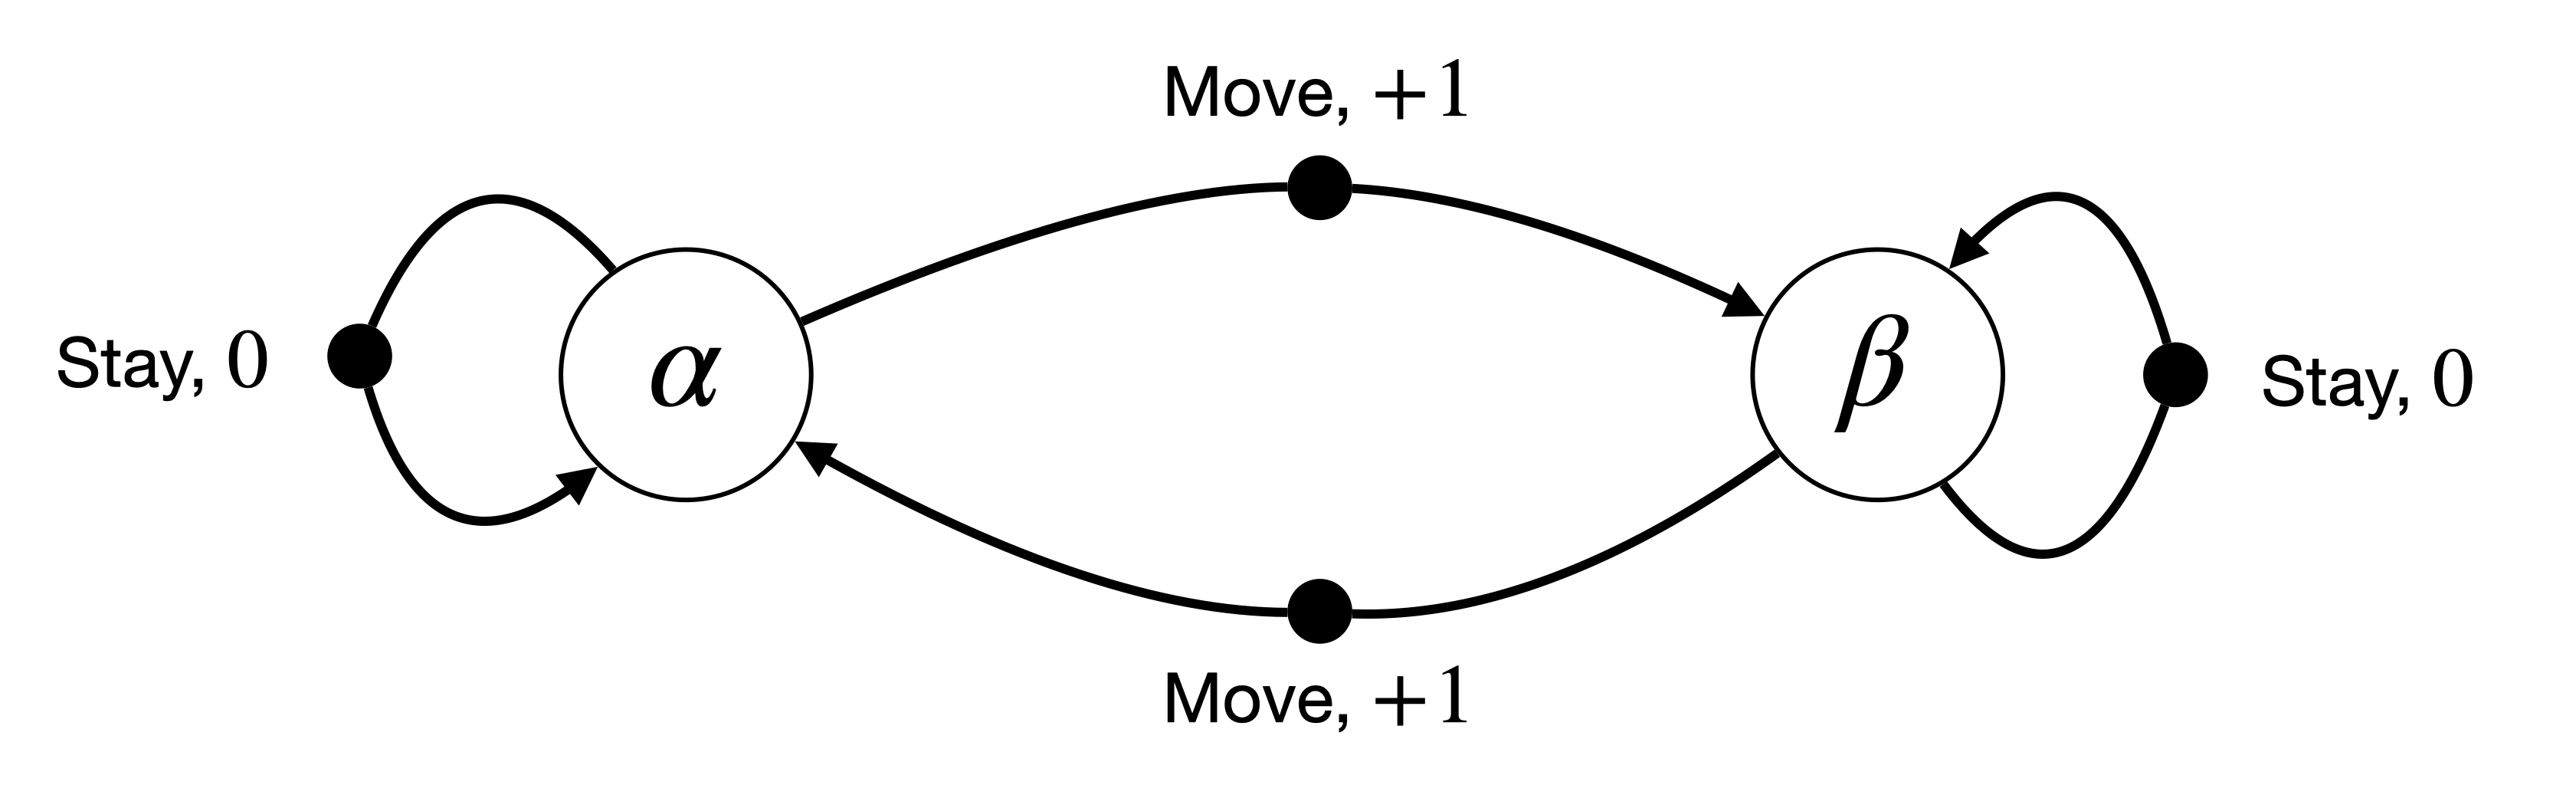
\includegraphics[width=0.9\linewidth]{images/MDP/robot-mdp-graph} 

}

\caption{A Simple Transition Graph.}\label{fig:mdp-robot-transition-graph}
\end{figure}

At time \(t=0\), if the robot starts at \(s_0 = \alpha\), first chooses action \(a_0 = \text{Move}\), and then chooses action \(a_1 = \text{Stay}\), the resulting trajectory is
\[
\tau = (\alpha, \text{Move}, +1, \beta, \text{Stay}, 0,  \beta).
\]
The return of this trajectory is:
\[
g_0 = +1 + 0 = +1.
\]

\textbf{Policy Evaluation}. Given a policy
\begin{equation}
\pi = (\pi_0, \pi_1), \quad \pi_0(a \mid s) = \begin{cases}
0.5 & a = \text{Move} \\
0.5 & a = \text{Stay}
\end{cases}, 
\quad 
\pi_1( a \mid s) = \begin{cases}
0.8 & a = \text{Move} \\
0.2 & a = \text{Stay}
\end{cases}.
\end{equation}
We can use the Bellman consistency equations to compute the state-value function. We first initialize:
\[
V^{\pi}_2 = \begin{bmatrix}
0 \\ 0
\end{bmatrix},
\]
where the first row contains the value at \(s = \alpha\) and the second row contains the value at \(s = \beta\).
We then perform the backward recursion for \(t=1\). For \(s = \alpha\), we have
\begin{equation}
V^{\pi}_1(\alpha) = \begin{bmatrix}
\pi_1(\text{Move} \mid \alpha) \\
\pi_1(\text{Stay} \mid \alpha)
\end{bmatrix}^{\top} \begin{bmatrix}
R(\alpha, \text{Move}) + V^{\pi}_2(\beta) \\
R(\alpha, \text{Stay}) + V^{\pi}_2(\alpha)
\end{bmatrix} = \begin{bmatrix}
0.8 \\ 0.2
\end{bmatrix}^{\top}
\begin{bmatrix}
1 \\ 0
\end{bmatrix} = 0.8 
\end{equation}
For \(s = \beta\), we have
\begin{equation}
V^{\pi}_1(\beta) = \begin{bmatrix}
\pi_1(\text{Move} \mid \beta) \\
\pi_1(\text{Stay} \mid \beta)
\end{bmatrix}^{\top} \begin{bmatrix}
R(\beta, \text{Move}) + V^{\pi}_2(\alpha) \\
R(\beta, \text{Stay}) + V^{\pi}_2(\beta)
\end{bmatrix} = \begin{bmatrix}
0.8 \\ 0.2
\end{bmatrix}^{\top}
\begin{bmatrix}
1 \\ 0
\end{bmatrix} = 0.8.
\end{equation}
Therefore, we have
\[
V^{\pi}_1 = \begin{bmatrix}
0.8 \\ 0.8
\end{bmatrix}.
\]
We then proceed to the backward recursion for \(t=0\):
\begin{align}
V_0^{\pi}(\alpha) & = \begin{bmatrix}
\pi_0(\text{Move} \mid \alpha) \\
\pi_0(\text{Stay} \mid \alpha)
\end{bmatrix}^{\top} \begin{bmatrix}
R(\alpha, \text{Move}) + V^{\pi}_1(\beta) \\
R(\alpha, \text{Stay}) + V^{\pi}_1(\alpha)
\end{bmatrix} = \begin{bmatrix}
0.5 \\ 0.5
\end{bmatrix}^{\top}
\begin{bmatrix}
1.8 \\ 0.8
\end{bmatrix} = 1.3. \\
V_0^{\pi}(\beta) & = \begin{bmatrix}
\pi_0(\text{Move} \mid \beta) \\
\pi_0(\text{Stay} \mid \beta)
\end{bmatrix}^{\top} \begin{bmatrix}
R(\beta, \text{Move}) + V^{\pi}_0(\alpha) \\
R(\beta, \text{Stay}) + V^{\pi}_0(\beta)
\end{bmatrix} = \begin{bmatrix}
0.5 \\ 0.5
\end{bmatrix}^{\top}
\begin{bmatrix}
1.8 \\ 0.8
\end{bmatrix} = 1.3.
\end{align}
Therefore, the state-value function at \(t=0\) is
\[
V^{\pi}_0 = \begin{bmatrix}
1.3 \\ 1.3
\end{bmatrix}.
\]
You are encouraged to carry out the similar calculations for the action-value function.

\begin{center}\rule{0.5\linewidth}{0.5pt}\end{center}

The toy example was small enough to carry out policy evaluation by hand; in realistic MDPs, we will need the help from computers.

Consider now an MDP whose transition graph is shown in Fig. \ref{fig:mdp-hangover-transition-graph}. This example is adapted from \href{https://github.com/upb-lea/reinforcement_learning_course_materials/blob/master/exercises/solutions/ex02/Ex2.ipynb}{here}.

\begin{figure}

{\centering 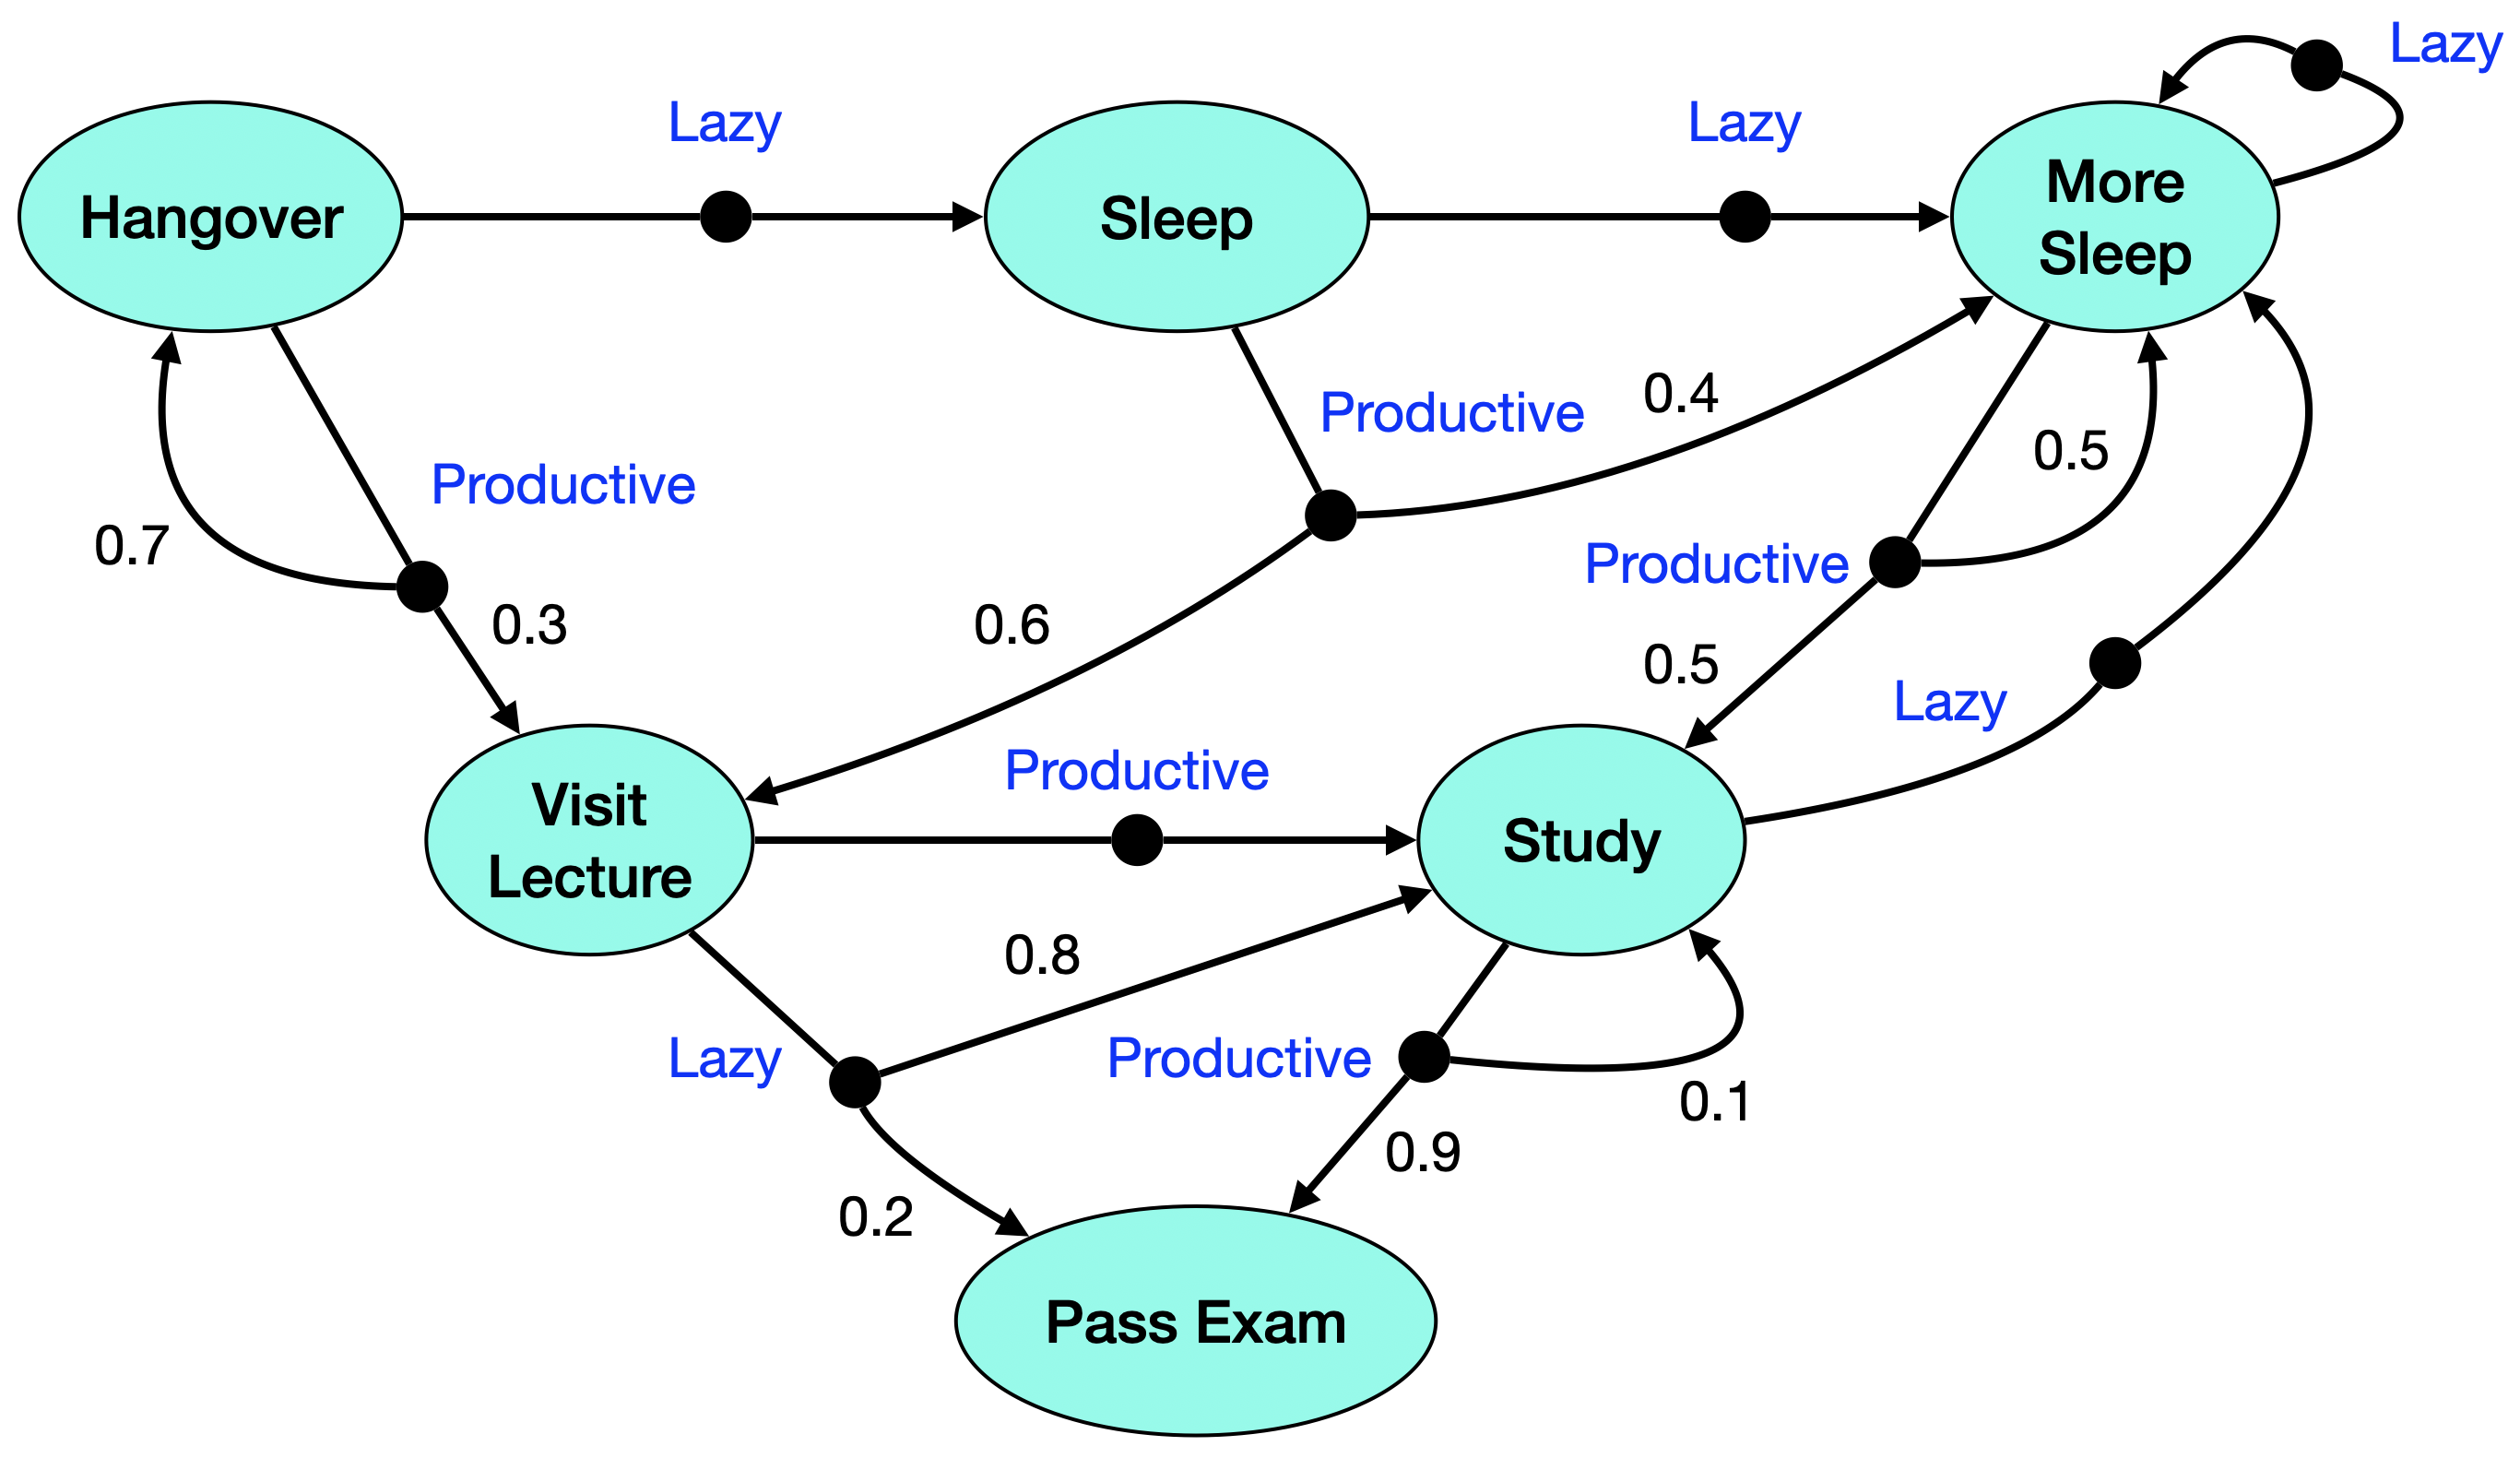
\includegraphics[width=0.9\linewidth]{images/MDP/hangover-graph} 

}

\caption{Hangover Transition Graph.}\label{fig:mdp-hangover-transition-graph}
\end{figure}

This MDP has six states:
\[
\mathcal{S} = \{\text{Hangover}, \text{Sleep}, \text{More Sleep}, \text{Visit Lecture}, \text{Study}, \text{Pass Exam} \},
\]
and two actions:
\[
\mathcal{A} = \{\text{Lazy}, \text{Productive} \}.
\]
The stochastic transition dynamics are labeled in the transition graph. For example, at state ``Hangover'', taking action ``Productive'' will lead to state ``Visit Lecture'' with probability \(0.3\) and state ``Hangover'' with probability \(0.7\).
The rewards of the MDP are defined as:
\[
R(s,a) = \begin{cases}
+1 & s = \text{Pass Exam} \\
-1 & \text{otherwise}.
\end{cases}.
\]

\textbf{Policy Evaluation}. Consider a time-invariant random policy
\[
\pi = \{\pi_0,\dots,\pi_{T-1} \}, \quad \pi_t(a \mid s) = \begin{cases}
\alpha & a = \text{Lazy} \\
1 - \alpha & a = \text{Productive}
\end{cases},
\]
that takes ``Lazy'' with probability \(\alpha\) and ``Productive'' with probability \(1-\alpha\).

The following Python code performs policy evaluation for this MDP, with \(T=10\) and \(\alpha = 0.4\).

\begin{Shaded}
\begin{Highlighting}[]
\CommentTok{\# Finite{-}horizon policy evaluation for the Hangover MDP}

\ImportTok{from}\NormalTok{ collections }\ImportTok{import}\NormalTok{ defaultdict}
\ImportTok{from}\NormalTok{ typing }\ImportTok{import}\NormalTok{ Dict, List, Tuple}

\NormalTok{State }\OperatorTok{=} \BuiltInTok{str}
\NormalTok{Action }\OperatorTok{=} \BuiltInTok{str}

\CommentTok{\# {-}{-}{-} MDP spec {-}{-}{-}{-}{-}{-}{-}{-}{-}{-}{-}{-}{-}{-}{-}{-}{-}{-}{-}{-}{-}{-}{-}{-}{-}{-}{-}{-}{-}{-}{-}{-}{-}{-}{-}{-}{-}{-}{-}{-}{-}{-}{-}{-}{-}{-}{-}{-}{-}{-}{-}{-}{-}{-}{-}{-}{-}{-}{-}{-}{-}{-}{-}}

\NormalTok{S: List[State] }\OperatorTok{=}\NormalTok{ [}
    \StringTok{"Hangover"}\NormalTok{, }\StringTok{"Sleep"}\NormalTok{, }\StringTok{"More Sleep"}\NormalTok{, }\StringTok{"Visit Lecture"}\NormalTok{, }\StringTok{"Study"}\NormalTok{, }\StringTok{"Pass Exam"}
\NormalTok{]}
\NormalTok{A: List[Action] }\OperatorTok{=}\NormalTok{ [}\StringTok{"Lazy"}\NormalTok{, }\StringTok{"Productive"}\NormalTok{]}

\CommentTok{\# P[s, a] {-}\textgreater{} list of (s\_next, prob)}
\NormalTok{P: Dict[Tuple[State, Action], List[Tuple[State, }\BuiltInTok{float}\NormalTok{]]] }\OperatorTok{=}\NormalTok{ \{}
    \CommentTok{\# Hangover}
\NormalTok{    (}\StringTok{"Hangover"}\NormalTok{, }\StringTok{"Lazy"}\NormalTok{):       [(}\StringTok{"Sleep"}\NormalTok{, }\FloatTok{1.0}\NormalTok{)],}
\NormalTok{    (}\StringTok{"Hangover"}\NormalTok{, }\StringTok{"Productive"}\NormalTok{): [(}\StringTok{"Visit Lecture"}\NormalTok{, }\FloatTok{0.3}\NormalTok{), (}\StringTok{"Hangover"}\NormalTok{, }\FloatTok{0.7}\NormalTok{)],}

    \CommentTok{\# Sleep}
\NormalTok{    (}\StringTok{"Sleep"}\NormalTok{, }\StringTok{"Lazy"}\NormalTok{):          [(}\StringTok{"More Sleep"}\NormalTok{, }\FloatTok{1.0}\NormalTok{)],}
\NormalTok{    (}\StringTok{"Sleep"}\NormalTok{, }\StringTok{"Productive"}\NormalTok{):    [(}\StringTok{"Visit Lecture"}\NormalTok{, }\FloatTok{0.6}\NormalTok{), (}\StringTok{"More Sleep"}\NormalTok{, }\FloatTok{0.4}\NormalTok{)],}

    \CommentTok{\# More Sleep}
\NormalTok{    (}\StringTok{"More Sleep"}\NormalTok{, }\StringTok{"Lazy"}\NormalTok{):       [(}\StringTok{"More Sleep"}\NormalTok{, }\FloatTok{1.0}\NormalTok{)],}
\NormalTok{    (}\StringTok{"More Sleep"}\NormalTok{, }\StringTok{"Productive"}\NormalTok{): [(}\StringTok{"Study"}\NormalTok{, }\FloatTok{0.5}\NormalTok{), (}\StringTok{"More Sleep"}\NormalTok{, }\FloatTok{0.5}\NormalTok{)],}

    \CommentTok{\# Visit Lecture}
\NormalTok{    (}\StringTok{"Visit Lecture"}\NormalTok{, }\StringTok{"Lazy"}\NormalTok{):       [(}\StringTok{"Study"}\NormalTok{, }\FloatTok{0.8}\NormalTok{), (}\StringTok{"Pass Exam"}\NormalTok{, }\FloatTok{0.2}\NormalTok{)],}
\NormalTok{    (}\StringTok{"Visit Lecture"}\NormalTok{, }\StringTok{"Productive"}\NormalTok{): [(}\StringTok{"Study"}\NormalTok{, }\FloatTok{1.0}\NormalTok{)],}

    \CommentTok{\# Study}
\NormalTok{    (}\StringTok{"Study"}\NormalTok{, }\StringTok{"Lazy"}\NormalTok{):         [(}\StringTok{"More Sleep"}\NormalTok{, }\FloatTok{1.0}\NormalTok{)],}
\NormalTok{    (}\StringTok{"Study"}\NormalTok{, }\StringTok{"Productive"}\NormalTok{):   [(}\StringTok{"Pass Exam"}\NormalTok{, }\FloatTok{0.9}\NormalTok{), (}\StringTok{"Study"}\NormalTok{, }\FloatTok{0.1}\NormalTok{)],}

    \CommentTok{\# Pass Exam (absorbing)}
\NormalTok{    (}\StringTok{"Pass Exam"}\NormalTok{, }\StringTok{"Lazy"}\NormalTok{):       [(}\StringTok{"Pass Exam"}\NormalTok{, }\FloatTok{1.0}\NormalTok{)],}
\NormalTok{    (}\StringTok{"Pass Exam"}\NormalTok{, }\StringTok{"Productive"}\NormalTok{): [(}\StringTok{"Pass Exam"}\NormalTok{, }\FloatTok{1.0}\NormalTok{)],}
\NormalTok{\}}

\KeywordTok{def}\NormalTok{ R(s: State, a: Action) }\OperatorTok{{-}\textgreater{}} \BuiltInTok{float}\NormalTok{:}
    \CommentTok{"""Reward: +1 in Pass Exam, {-}1 otherwise."""}
    \ControlFlowTok{return} \FloatTok{1.0} \ControlFlowTok{if}\NormalTok{ s }\OperatorTok{==} \StringTok{"Pass Exam"} \ControlFlowTok{else} \OperatorTok{{-}}\FloatTok{1.0}

\CommentTok{\# {-}{-}{-} Policy: time{-}invariant, state{-}independent {-}{-}{-}{-}{-}{-}{-}{-}{-}{-}{-}{-}{-}{-}{-}{-}{-}{-}{-}{-}{-}{-}{-}{-}{-}{-}{-}{-}{-}{-}}

\KeywordTok{def}\NormalTok{ pi(a: Action, s: State, alpha: }\BuiltInTok{float}\NormalTok{) }\OperatorTok{{-}\textgreater{}} \BuiltInTok{float}\NormalTok{:}
    \CommentTok{"""pi(a|s): Lazy with prob alpha, Productive with prob 1{-}alpha."""}
    \ControlFlowTok{return}\NormalTok{ alpha }\ControlFlowTok{if}\NormalTok{ a }\OperatorTok{==} \StringTok{"Lazy"} \ControlFlowTok{else}\NormalTok{ (}\FloatTok{1.0} \OperatorTok{{-}}\NormalTok{ alpha)}

\CommentTok{\# {-}{-}{-} Policy evaluation {-}{-}{-}{-}{-}{-}{-}{-}{-}{-}{-}{-}{-}{-}{-}{-}{-}{-}{-}{-}{-}{-}{-}{-}{-}{-}{-}{-}{-}{-}{-}{-}{-}{-}{-}{-}{-}{-}{-}{-}{-}{-}{-}{-}{-}{-}{-}{-}{-}{-}{-}{-}{-}{-}{-}}

\KeywordTok{def}\NormalTok{ policy\_evaluation(T: }\BuiltInTok{int}\NormalTok{, alpha: }\BuiltInTok{float}\NormalTok{):}
    \CommentTok{"""}
\CommentTok{    Compute \{V\_t(s)\} and \{Q\_t(s,a)\} for t=0..T with terminal condition V\_T = Q\_T = 0.}
\CommentTok{    Returns:}
\CommentTok{        V: Dict[int, Dict[State, float]]}
\CommentTok{        Q: Dict[int, Dict[Tuple[State, Action], float]]}
\CommentTok{    """}
    \ControlFlowTok{assert}\NormalTok{ T }\OperatorTok{\textgreater{}=} \DecValTok{0}
    \CommentTok{\# sanity: probabilities sum to 1 for each (s,a)}
    \ControlFlowTok{for}\NormalTok{ key, rows }\KeywordTok{in}\NormalTok{ P.items():}
\NormalTok{        total }\OperatorTok{=} \BuiltInTok{sum}\NormalTok{(p }\ControlFlowTok{for}\NormalTok{ \_, p }\KeywordTok{in}\NormalTok{ rows)}
        \ControlFlowTok{if} \BuiltInTok{abs}\NormalTok{(total }\OperatorTok{{-}} \FloatTok{1.0}\NormalTok{) }\OperatorTok{\textgreater{}} \FloatTok{1e{-}9}\NormalTok{:}
            \ControlFlowTok{raise} \PreprocessorTok{ValueError}\NormalTok{(}\SpecialStringTok{f"Probabilities for }\SpecialCharTok{\{}\NormalTok{key}\SpecialCharTok{\}}\SpecialStringTok{ sum to }\SpecialCharTok{\{}\NormalTok{total}\SpecialCharTok{\}}\SpecialStringTok{, not 1."}\NormalTok{)}

\NormalTok{    V: Dict[}\BuiltInTok{int}\NormalTok{, Dict[State, }\BuiltInTok{float}\NormalTok{]] }\OperatorTok{=}\NormalTok{ defaultdict(}\BuiltInTok{dict}\NormalTok{)}
\NormalTok{    Q: Dict[}\BuiltInTok{int}\NormalTok{, Dict[Tuple[State, Action], }\BuiltInTok{float}\NormalTok{]] }\OperatorTok{=}\NormalTok{ defaultdict(}\BuiltInTok{dict}\NormalTok{)}

    \CommentTok{\# Terminal boundary}
    \ControlFlowTok{for}\NormalTok{ s }\KeywordTok{in}\NormalTok{ S:}
\NormalTok{        V[T][s] }\OperatorTok{=} \FloatTok{0.0}
        \ControlFlowTok{for}\NormalTok{ a }\KeywordTok{in}\NormalTok{ A:}
\NormalTok{            Q[T][(s, a)] }\OperatorTok{=} \FloatTok{0.0}

    \CommentTok{\# Backward recursion}
    \ControlFlowTok{for}\NormalTok{ t }\KeywordTok{in} \BuiltInTok{range}\NormalTok{(T }\OperatorTok{{-}} \DecValTok{1}\NormalTok{, }\OperatorTok{{-}}\DecValTok{1}\NormalTok{, }\OperatorTok{{-}}\DecValTok{1}\NormalTok{):}
        \ControlFlowTok{for}\NormalTok{ s }\KeywordTok{in}\NormalTok{ S:}
            \CommentTok{\# First compute Q\_t(s,a)}
            \ControlFlowTok{for}\NormalTok{ a }\KeywordTok{in}\NormalTok{ A:}
\NormalTok{                exp\_next }\OperatorTok{=} \BuiltInTok{sum}\NormalTok{(p }\OperatorTok{*}\NormalTok{ V[t }\OperatorTok{+} \DecValTok{1}\NormalTok{][s\_next] }\ControlFlowTok{for}\NormalTok{ s\_next, p }\KeywordTok{in}\NormalTok{ P[(s, a)])}
\NormalTok{                Q[t][(s, a)] }\OperatorTok{=}\NormalTok{ R(s, a) }\OperatorTok{+}\NormalTok{ exp\_next}
            \CommentTok{\# Then V\_t(s) = E\_\{a\textasciitilde{}pi\}[Q\_t(s,a)]}
\NormalTok{            V[t][s] }\OperatorTok{=} \BuiltInTok{sum}\NormalTok{(pi(a, s, alpha) }\OperatorTok{*}\NormalTok{ Q[t][(s, a)] }\ControlFlowTok{for}\NormalTok{ a }\KeywordTok{in}\NormalTok{ A)}

    \ControlFlowTok{return}\NormalTok{ V, Q}

\CommentTok{\# {-}{-}{-} Example run {-}{-}{-}{-}{-}{-}{-}{-}{-}{-}{-}{-}{-}{-}{-}{-}{-}{-}{-}{-}{-}{-}{-}{-}{-}{-}{-}{-}{-}{-}{-}{-}{-}{-}{-}{-}{-}{-}{-}{-}{-}{-}{-}{-}{-}{-}{-}{-}{-}{-}{-}{-}{-}{-}{-}{-}{-}{-}{-}{-}{-}}

\ControlFlowTok{if} \VariableTok{\_\_name\_\_} \OperatorTok{==} \StringTok{"\_\_main\_\_"}\NormalTok{:}
\NormalTok{    T }\OperatorTok{=} \DecValTok{10}        \CommentTok{\# horizon}
\NormalTok{    alpha }\OperatorTok{=} \FloatTok{0.4}  \CommentTok{\# probability of choosing Lazy}
\NormalTok{    V, Q }\OperatorTok{=}\NormalTok{ policy\_evaluation(T}\OperatorTok{=}\NormalTok{T, alpha}\OperatorTok{=}\NormalTok{alpha)}

    \CommentTok{\# Print V\_0}
    \BuiltInTok{print}\NormalTok{(}\SpecialStringTok{f"V\_0(s) with T=}\SpecialCharTok{\{}\NormalTok{T}\SpecialCharTok{\}}\SpecialStringTok{, alpha=}\SpecialCharTok{\{}\NormalTok{alpha}\SpecialCharTok{\}}\SpecialStringTok{:"}\NormalTok{)}
    \ControlFlowTok{for}\NormalTok{ s }\KeywordTok{in}\NormalTok{ S:}
        \BuiltInTok{print}\NormalTok{(}\SpecialStringTok{f"  }\SpecialCharTok{\{}\NormalTok{s}\SpecialCharTok{:13s\}}\SpecialStringTok{: }\SpecialCharTok{\{}\NormalTok{V[}\DecValTok{0}\NormalTok{][s]}\SpecialCharTok{: .3f\}}\SpecialStringTok{"}\NormalTok{)}
\end{Highlighting}
\end{Shaded}

The code returns the following state values at \(t=0\):
\begin{equation}
V^{\pi}_0 = \begin{bmatrix}
-3.582 \\ -2.306 \\ -2.180 \\ 1.757 \\ 2.939 \\ 10
\end{bmatrix},
\label{eq:HangoverRandomValueFunction}
\end{equation}
where the ordering of the states follows that defined in \(\mathcal{S}\).

You can find the code \href{https://github.com/ComputationalRobotics/2025-ES-AM-158-LECTURE-CODE/blob/main/hangover_policy_evaluation.py}{here}.
\end{example}

\subsection{Principle of Optimality}\label{optimality}

Every policy \(\pi\) induces a value function \(V_0^{\pi}\) that can be evaluated by policy evaluation (assuming the transition dynamics are known). The goal of reinforcement learning is to find an optimal policy that maximizes the value function with respect to a given initial state distribution:
\begin{equation}
V^\star_0 = \max_{\pi}\; \mathbb{E}_{s_0 \sim \mu(\cdot)} \big[ V_0^{\pi}(s_0) \big],
\label{eq:FiniteHorizonMDPRLProblem}
\end{equation}
where we have used the superscript ``\(\star\)'' to denote the optimality of the value function. \(V^\star_0\) is often known as the \emph{optimal value function}.

At first glance, \eqref{eq:FiniteHorizonMDPRLProblem} appears daunting: a naive approach would enumerate all stochastic policies \(\pi\), evaluate their value functions, and select the best. A central result in reinforcement learning and optimal control---rooted in the principle of optimality---is that the \emph{optimal} value functions satisfy a Bellman-style recursion, analogous to Proposition \ref{prp:BellmanConsistency}. This Bellman optimality recursion enables backward computation of the optimal value functions without enumerating policies.

\begin{theorem}[Bellman Optimality (Finite Horizon, State-Value)]
\protect\hypertarget{thm:FiniteHorizonMDPBellmanOptimality}{}\label{thm:FiniteHorizonMDPBellmanOptimality}Consider a finite-horizon MDP \(\mathcal{M}=(\mathcal{S},\mathcal{A},P,R,T)\) with finite state and action sets and bounded rewards.
Define the optimal value functions \(\{V_t^\star\}_{t=0}^{T}\) by the following \emph{Bellman optimality} recursion
\begin{equation}
\begin{split}
V_T^\star(s)& \equiv 0, \\
V_t^\star(s)& = \max_{a\in\mathcal{A}}\Big\{ R(s,a)\;+\;\sum_{s'\in\mathcal{S}} P(s'\mid s,a)\,V_{t+1}^\star(s')\Big\},\ t=T-1,\ldots,0.
\end{split}
\label{eq:FiniteHorizonMDPBellmanOptimality}
\end{equation}
Then, the optimal value functions are optimal in the sense of \emph{statewise dominance}:
\begin{equation}
V_t^{\star}(s)\;\ge\; V_t^{\pi}(s)
\quad\text{for all policies }\pi,\; s\in\mathcal{S},\; t=0,\ldots,T.
\label{eq:FiniteHorizonMDPStatewiseDominance}
\end{equation}

Moreover, the deterministic policy
\(\pi^\star=(\pi^\star_0,\ldots,\pi^\star_{T-1})\) with
\begin{equation}
\begin{split}
\pi_t^\star(s)\;\in\;\arg\max_{a\in\mathcal{A}}
\Big\{ R(s,a)\;+\;\sum_{s'\in\mathcal{S}} P(s'\mid s,a)\,V_{t+1}^\star(s')\Big\}, \\
\text{for any } s\in\mathcal{S},\; t=0,\dots,T-1
\end{split}
\label{eq:FiniteHorizonMDPOptimalPolicy}
\end{equation}
is optimal, where ties can be broken by any fixed rule.
\end{theorem}

\begin{proof}
We first show that the value functions defined by the Bellman optimality recursion \eqref{eq:FiniteHorizonMDPBellmanOptimality} are \emph{optimal} in the sense that they dominate the value functions of any other policy. The proof proceeds by backward induction.

\textbf{Base case (\(t=T\)).}
For every \(s\in\mathcal{S}\),
\[
V^\star_T(s)\;=\;0\;=\;V_T^{\pi}(s),
\]
so \(V^\star_T(s)\ge V_T^{\pi}(s)\) holds trivially.

\textbf{Inductive step.}
Assume \(V^\star_{t+1}(s)\ge V^{\pi}_{t+1}(s)\) for all \(s\in\mathcal{S}\). Then, for any \(s\in\mathcal{S}\),
\begin{align*}
V_t^{\pi}(s)
&= \sum_{a\in\mathcal{A}} \pi_t(a\mid s)\!\left(R(s,a)+\sum_{s'\in\mathcal{S}} P(s'\mid s,a)\,V_{t+1}^{\pi}(s')\right) \\
&\le \sum_{a\in\mathcal{A}} \pi_t(a\mid s)\!\left(R(s,a)+\sum_{s'\in\mathcal{S}} P(s'\mid s,a)\,V_{t+1}^{\star}(s')\right) \\
&\le \max_{a\in\mathcal{A}} \left(R(s,a)+\sum_{s'\in\mathcal{S}} P(s'\mid s,a)\,V_{t+1}^{\star}(s')\right)
\;=\; V_t^\star(s),
\end{align*}
where the first inequality uses the induction hypothesis and the second uses that an expectation is bounded above by a maximum. Hence \(V_t^\star(s)\ge V_t^{\pi}(s)\) for all \(s\), completing the induction. Therefore, \(\{V_t^\star\}_{t=0}^T\) dominates the value functions attainable by any policy.

Next, we show that \(\{V_t^\star\}\) is \emph{attainable} by some policy. Since \(\mathcal{A}\) is finite (tabular setting), the maximizer in the Bellman optimality operator exists for every \((t,s)\); thus we can define a (deterministic) greedy policy
\[
\pi_t^\star(s)\;\in\;\arg\max_{a\in\mathcal{A}}
\Big\{ R(s,a)+\sum_{s'\in\mathcal{S}} P(s'\mid s,a)\,V_{t+1}^\star(s') \Big\}.
\]
A simple backward induction then shows \(V_t^{\pi^\star}(s)=V_t^\star(s)\) for all \(t\) and \(s\): at \(t=T\) both are \(0\), and if \(V_{t+1}^{\pi^\star}=V_{t+1}^\star\), then by construction of \(\pi_t^\star\) the Bellman equality yields \(V_t^{\pi^\star}=V_t^\star\). Consequently, the optimal value functions are achieved by the greedy (deterministic) policy \(\pi^\star\).
\end{proof}

\begin{corollary}[Bellman Optimality (Finite Horizon, Action-Value)]
\protect\hypertarget{cor:FiniteHorizonMDPBellmanOptimalityActionValue}{}\label{cor:FiniteHorizonMDPBellmanOptimalityActionValue}Given the optimal (state-)value functions \(V^{\star}_{t},t=0,\dots,T\), define the optimal action-value function
\begin{equation}
Q_t^\star(s,a)\;=\;R(s,a)+\sum_{s'\in\mathcal{S}} P(s'\mid s,a)\,V_{t+1}^\star(s'), \quad t=0,\dots,T-1.
\label{eq:FiniteHorizonMDPOptimalActionValue}
\end{equation}

Then we have
\begin{equation}
V_t^\star(s)=\max_{a\in\mathcal{A}} Q_t^\star(s,a),\qquad
\pi_t^\star(s)\in\arg\max_{a\in\mathcal{A}} Q_t^\star(s,a).
\label{eq:FiniteHorizonMDPStateValueActionValue}
\end{equation}

The optimal action-value functions satisfy:
\begin{equation}
\begin{split}
Q_T^\star(s,a) & \equiv 0,\\
Q_t^\star(s,a)
& = R(s,a) \;+\; \mathbb{E}_{s'\sim P(\cdot\mid s,a)}
\!\left[ \max_{a'\in\mathcal{A}} Q_{t+1}^\star(s',a') \right],
\quad t=T-1,\ldots,0.
\end{split}
\label{eq:FiniteHorizonMDPBellmanRecursionActionValue}
\end{equation}
\end{corollary}

\subsection{Dynamic Programming}\label{dp}

The principle of optimality in Theorem \ref{thm:FiniteHorizonMDPBellmanOptimality} yields a constructive procedure to compute the optimal value functions and an associated deterministic optimal policy. This backward-induction procedure is the \emph{dynamic programming} (DP) algorithm.

\textbf{Dynamic programming (finite horizon).}

\begin{itemize}
\item
  \textbf{Initialization.} Set \(V_T^\star(s) = 0\) for all \(s \in \mathcal{S}\).
\item
  \textbf{Backward recursion.} For \(t = T-1, T-2, \dots, 0\):

  \begin{itemize}
  \item
    \emph{Optimal value:} for each \(s \in \mathcal{S}\),
    \[
    V_t^\star(s)
    = \max_{a \in \mathcal{A}}
    \left\{
    R(s,a) + \mathbb{E}_{s' \sim P(\cdot \mid s,a)} \big[ V_{t+1}^\star(s') \big]
    \right\}.
    \]
  \item
    \emph{Greedy policy (deterministic):} for each \(s \in \mathcal{S}\),
    \[
    \pi_t^\star(s) \in \arg\max_{a \in \mathcal{A}}
    \left\{
    R(s,a) + \mathbb{E}_{s' \sim P(\cdot \mid s,a)} \big[ V_{t+1}^\star(s') \big]
    \right\}.
    \]
  \end{itemize}
\end{itemize}

\begin{exercise}
How does dynamic programming look like when applied to the action-value function?
\end{exercise}

\begin{exercise}
What is the computational complexity of dynamic programming?
\end{exercise}

Let us try dynamic programming for the Hangover MDP presented before.

\begin{example}[Dynamic Programming for Hangover MDP]
\protect\hypertarget{exm:HangoverDynamicProgramming}{}\label{exm:HangoverDynamicProgramming}Consider the Hangover MDP defined by the transition graph shown in Fig. \ref{fig:mdp-hangover-transition-graph}. With slight modification to the policy evaluation code, we can find the optimal value functions and optimal policies.

\begin{Shaded}
\begin{Highlighting}[]
\CommentTok{\# Dynamic programming (finite{-}horizon optimal control) for the Hangover MDP}

\ImportTok{from}\NormalTok{ collections }\ImportTok{import}\NormalTok{ defaultdict}
\ImportTok{from}\NormalTok{ typing }\ImportTok{import}\NormalTok{ Dict, List, Tuple}

\NormalTok{State }\OperatorTok{=} \BuiltInTok{str}
\NormalTok{Action }\OperatorTok{=} \BuiltInTok{str}

\CommentTok{\# {-}{-}{-} MDP spec {-}{-}{-}{-}{-}{-}{-}{-}{-}{-}{-}{-}{-}{-}{-}{-}{-}{-}{-}{-}{-}{-}{-}{-}{-}{-}{-}{-}{-}{-}{-}{-}{-}{-}{-}{-}{-}{-}{-}{-}{-}{-}{-}{-}{-}{-}{-}{-}{-}{-}{-}{-}{-}{-}{-}{-}{-}{-}{-}{-}{-}{-}{-}}

\NormalTok{S: List[State] }\OperatorTok{=}\NormalTok{ [}
    \StringTok{"Hangover"}\NormalTok{, }\StringTok{"Sleep"}\NormalTok{, }\StringTok{"More Sleep"}\NormalTok{, }\StringTok{"Visit Lecture"}\NormalTok{, }\StringTok{"Study"}\NormalTok{, }\StringTok{"Pass Exam"}
\NormalTok{]}
\NormalTok{A: List[Action] }\OperatorTok{=}\NormalTok{ [}\StringTok{"Lazy"}\NormalTok{, }\StringTok{"Productive"}\NormalTok{]}

\CommentTok{\# P[s, a] {-}\textgreater{} list of (s\_next, prob)}
\NormalTok{P: Dict[Tuple[State, Action], List[Tuple[State, }\BuiltInTok{float}\NormalTok{]]] }\OperatorTok{=}\NormalTok{ \{}
    \CommentTok{\# Hangover}
\NormalTok{    (}\StringTok{"Hangover"}\NormalTok{, }\StringTok{"Lazy"}\NormalTok{):       [(}\StringTok{"Sleep"}\NormalTok{, }\FloatTok{1.0}\NormalTok{)],}
\NormalTok{    (}\StringTok{"Hangover"}\NormalTok{, }\StringTok{"Productive"}\NormalTok{): [(}\StringTok{"Visit Lecture"}\NormalTok{, }\FloatTok{0.3}\NormalTok{), (}\StringTok{"Hangover"}\NormalTok{, }\FloatTok{0.7}\NormalTok{)],}

    \CommentTok{\# Sleep}
\NormalTok{    (}\StringTok{"Sleep"}\NormalTok{, }\StringTok{"Lazy"}\NormalTok{):          [(}\StringTok{"More Sleep"}\NormalTok{, }\FloatTok{1.0}\NormalTok{)],}
\NormalTok{    (}\StringTok{"Sleep"}\NormalTok{, }\StringTok{"Productive"}\NormalTok{):    [(}\StringTok{"Visit Lecture"}\NormalTok{, }\FloatTok{0.6}\NormalTok{), (}\StringTok{"More Sleep"}\NormalTok{, }\FloatTok{0.4}\NormalTok{)],}

    \CommentTok{\# More Sleep}
\NormalTok{    (}\StringTok{"More Sleep"}\NormalTok{, }\StringTok{"Lazy"}\NormalTok{):       [(}\StringTok{"More Sleep"}\NormalTok{, }\FloatTok{1.0}\NormalTok{)],}
\NormalTok{    (}\StringTok{"More Sleep"}\NormalTok{, }\StringTok{"Productive"}\NormalTok{): [(}\StringTok{"Study"}\NormalTok{, }\FloatTok{0.5}\NormalTok{), (}\StringTok{"More Sleep"}\NormalTok{, }\FloatTok{0.5}\NormalTok{)],}

    \CommentTok{\# Visit Lecture}
\NormalTok{    (}\StringTok{"Visit Lecture"}\NormalTok{, }\StringTok{"Lazy"}\NormalTok{):       [(}\StringTok{"Study"}\NormalTok{, }\FloatTok{0.8}\NormalTok{), (}\StringTok{"Pass Exam"}\NormalTok{, }\FloatTok{0.2}\NormalTok{)],}
\NormalTok{    (}\StringTok{"Visit Lecture"}\NormalTok{, }\StringTok{"Productive"}\NormalTok{): [(}\StringTok{"Study"}\NormalTok{, }\FloatTok{1.0}\NormalTok{)],}

    \CommentTok{\# Study}
\NormalTok{    (}\StringTok{"Study"}\NormalTok{, }\StringTok{"Lazy"}\NormalTok{):         [(}\StringTok{"More Sleep"}\NormalTok{, }\FloatTok{1.0}\NormalTok{)],}
\NormalTok{    (}\StringTok{"Study"}\NormalTok{, }\StringTok{"Productive"}\NormalTok{):   [(}\StringTok{"Pass Exam"}\NormalTok{, }\FloatTok{0.9}\NormalTok{), (}\StringTok{"Study"}\NormalTok{, }\FloatTok{0.1}\NormalTok{)],}

    \CommentTok{\# Pass Exam (absorbing)}
\NormalTok{    (}\StringTok{"Pass Exam"}\NormalTok{, }\StringTok{"Lazy"}\NormalTok{):       [(}\StringTok{"Pass Exam"}\NormalTok{, }\FloatTok{1.0}\NormalTok{)],}
\NormalTok{    (}\StringTok{"Pass Exam"}\NormalTok{, }\StringTok{"Productive"}\NormalTok{): [(}\StringTok{"Pass Exam"}\NormalTok{, }\FloatTok{1.0}\NormalTok{)],}
\NormalTok{\}}

\KeywordTok{def}\NormalTok{ R(s: State, a: Action) }\OperatorTok{{-}\textgreater{}} \BuiltInTok{float}\NormalTok{:}
    \CommentTok{"""Reward: +1 in Pass Exam, {-}1 otherwise."""}
    \ControlFlowTok{return} \FloatTok{1.0} \ControlFlowTok{if}\NormalTok{ s }\OperatorTok{==} \StringTok{"Pass Exam"} \ControlFlowTok{else} \OperatorTok{{-}}\FloatTok{1.0}

\CommentTok{\# {-}{-}{-} Dynamic programming (Bellman optimality) {-}{-}{-}{-}{-}{-}{-}{-}{-}{-}{-}{-}{-}{-}{-}{-}{-}{-}{-}{-}{-}{-}{-}{-}{-}{-}{-}{-}{-}{-}{-}}

\KeywordTok{def}\NormalTok{ dynamic\_programming(T: }\BuiltInTok{int}\NormalTok{):}
    \CommentTok{"""}
\CommentTok{    Compute optimal finite{-}horizon tables:}
\CommentTok{      {-} V[t][s] = V\_t\^{}*(s)}
\CommentTok{      {-} Q[t][(s,a)] = Q\_t\^{}*(s,a)}
\CommentTok{      {-} PI[t][s] = optimal action at (t,s)}
\CommentTok{    with terminal condition V\_T\^{}* = 0.}
\CommentTok{    """}
    \ControlFlowTok{assert}\NormalTok{ T }\OperatorTok{\textgreater{}=} \DecValTok{0}

    \CommentTok{\# sanity: probabilities sum to 1 for each (s,a)}
    \ControlFlowTok{for}\NormalTok{ key, rows }\KeywordTok{in}\NormalTok{ P.items():}
\NormalTok{        total }\OperatorTok{=} \BuiltInTok{sum}\NormalTok{(p }\ControlFlowTok{for}\NormalTok{ \_, p }\KeywordTok{in}\NormalTok{ rows)}
        \ControlFlowTok{if} \BuiltInTok{abs}\NormalTok{(total }\OperatorTok{{-}} \FloatTok{1.0}\NormalTok{) }\OperatorTok{\textgreater{}} \FloatTok{1e{-}9}\NormalTok{:}
            \ControlFlowTok{raise} \PreprocessorTok{ValueError}\NormalTok{(}\SpecialStringTok{f"Probabilities for }\SpecialCharTok{\{}\NormalTok{key}\SpecialCharTok{\}}\SpecialStringTok{ sum to }\SpecialCharTok{\{}\NormalTok{total}\SpecialCharTok{\}}\SpecialStringTok{, not 1."}\NormalTok{)}

\NormalTok{    V: Dict[}\BuiltInTok{int}\NormalTok{, Dict[State, }\BuiltInTok{float}\NormalTok{]] }\OperatorTok{=}\NormalTok{ defaultdict(}\BuiltInTok{dict}\NormalTok{)}
\NormalTok{    Q: Dict[}\BuiltInTok{int}\NormalTok{, Dict[Tuple[State, Action], }\BuiltInTok{float}\NormalTok{]] }\OperatorTok{=}\NormalTok{ defaultdict(}\BuiltInTok{dict}\NormalTok{)}
\NormalTok{    PI: Dict[}\BuiltInTok{int}\NormalTok{, Dict[State, Action]] }\OperatorTok{=}\NormalTok{ defaultdict(}\BuiltInTok{dict}\NormalTok{)}

    \CommentTok{\# Terminal boundary}
    \ControlFlowTok{for}\NormalTok{ s }\KeywordTok{in}\NormalTok{ S:}
\NormalTok{        V[T][s] }\OperatorTok{=} \FloatTok{0.0}
        \ControlFlowTok{for}\NormalTok{ a }\KeywordTok{in}\NormalTok{ A:}
\NormalTok{            Q[T][(s, a)] }\OperatorTok{=} \FloatTok{0.0}

    \CommentTok{\# Backward recursion (Bellman optimality)}
    \ControlFlowTok{for}\NormalTok{ t }\KeywordTok{in} \BuiltInTok{range}\NormalTok{(T }\OperatorTok{{-}} \DecValTok{1}\NormalTok{, }\OperatorTok{{-}}\DecValTok{1}\NormalTok{, }\OperatorTok{{-}}\DecValTok{1}\NormalTok{):}
        \ControlFlowTok{for}\NormalTok{ s }\KeywordTok{in}\NormalTok{ S:}
            \CommentTok{\# compute Q*\_t(s,a)}
            \ControlFlowTok{for}\NormalTok{ a }\KeywordTok{in}\NormalTok{ A:}
\NormalTok{                exp\_next }\OperatorTok{=} \BuiltInTok{sum}\NormalTok{(p }\OperatorTok{*}\NormalTok{ V[t }\OperatorTok{+} \DecValTok{1}\NormalTok{][s\_next] }\ControlFlowTok{for}\NormalTok{ s\_next, p }\KeywordTok{in}\NormalTok{ P[(s, a)])}
\NormalTok{                Q[t][(s, a)] }\OperatorTok{=}\NormalTok{ R(s, a) }\OperatorTok{+}\NormalTok{ exp\_next}

            \CommentTok{\# greedy action and optimal value}
            \CommentTok{\# tie{-}breaking is deterministic by the order in A}
\NormalTok{            best\_a }\OperatorTok{=} \BuiltInTok{max}\NormalTok{(A, key}\OperatorTok{=}\KeywordTok{lambda}\NormalTok{ a: Q[t][(s, a)])}
\NormalTok{            PI[t][s] }\OperatorTok{=}\NormalTok{ best\_a}
\NormalTok{            V[t][s] }\OperatorTok{=}\NormalTok{ Q[t][(s, best\_a)]}

    \ControlFlowTok{return}\NormalTok{ V, Q, PI}

\CommentTok{\# {-}{-}{-} Example run {-}{-}{-}{-}{-}{-}{-}{-}{-}{-}{-}{-}{-}{-}{-}{-}{-}{-}{-}{-}{-}{-}{-}{-}{-}{-}{-}{-}{-}{-}{-}{-}{-}{-}{-}{-}{-}{-}{-}{-}{-}{-}{-}{-}{-}{-}{-}{-}{-}{-}{-}{-}{-}{-}{-}{-}{-}{-}{-}{-}{-}}

\ControlFlowTok{if} \VariableTok{\_\_name\_\_} \OperatorTok{==} \StringTok{"\_\_main\_\_"}\NormalTok{:}
\NormalTok{    T }\OperatorTok{=} \DecValTok{10}  \CommentTok{\# horizon}
\NormalTok{    V, Q, PI }\OperatorTok{=}\NormalTok{ dynamic\_programming(T}\OperatorTok{=}\NormalTok{T)}

    \BuiltInTok{print}\NormalTok{(}\SpecialStringTok{f"Optimal V\_0(s) with T=}\SpecialCharTok{\{}\NormalTok{T}\SpecialCharTok{\}}\SpecialStringTok{:"}\NormalTok{)}
    \ControlFlowTok{for}\NormalTok{ s }\KeywordTok{in}\NormalTok{ S:}
        \BuiltInTok{print}\NormalTok{(}\SpecialStringTok{f"  }\SpecialCharTok{\{}\NormalTok{s}\SpecialCharTok{:13s\}}\SpecialStringTok{: }\SpecialCharTok{\{}\NormalTok{V[}\DecValTok{0}\NormalTok{][s]}\SpecialCharTok{: .3f\}}\SpecialStringTok{"}\NormalTok{)}

    \BuiltInTok{print}\NormalTok{(}\StringTok{"}\CharTok{\textbackslash{}n}\StringTok{Greedy policy at t=0:"}\NormalTok{)}
    \ControlFlowTok{for}\NormalTok{ s }\KeywordTok{in}\NormalTok{ S:}
        \BuiltInTok{print}\NormalTok{(}\SpecialStringTok{f"  }\SpecialCharTok{\{}\NormalTok{s}\SpecialCharTok{:13s\}}\SpecialStringTok{: }\SpecialCharTok{\{}\NormalTok{PI[}\DecValTok{0}\NormalTok{][s]}\SpecialCharTok{\}}\SpecialStringTok{"}\NormalTok{)}

    \BuiltInTok{print}\NormalTok{(}\StringTok{"}\CharTok{\textbackslash{}n}\StringTok{Action value at t=0:"}\NormalTok{)}
    \ControlFlowTok{for}\NormalTok{ s }\KeywordTok{in}\NormalTok{ S:}
        \BuiltInTok{print}\NormalTok{(}\SpecialStringTok{f"  }\SpecialCharTok{\{}\NormalTok{s}\SpecialCharTok{:13s\}}\SpecialStringTok{: }\SpecialCharTok{\{}\NormalTok{Q[}\DecValTok{0}\NormalTok{][s, A[}\DecValTok{0}\NormalTok{]]}\SpecialCharTok{: .3f\}}\SpecialStringTok{, }\SpecialCharTok{\{}\NormalTok{Q[}\DecValTok{0}\NormalTok{][s, A[}\DecValTok{1}\NormalTok{]]}\SpecialCharTok{: .3f\}}\SpecialStringTok{"}\NormalTok{)}
\end{Highlighting}
\end{Shaded}

The optimal value function at \(t=0\) is:
\begin{equation}
V^\star_0 = \begin{bmatrix}
1.259 \\
3.251 \\
3.787 \\
6.222 \\
7.778 \\
10
\end{bmatrix}.
\label{eq:HangoverOptimalValueFunction}
\end{equation}
Clearly, the optimal value function dominates the value function shown in \eqref{eq:HangoverRandomValueFunction} of the random policy at every state.

The optimal actions at \(t=0\) are:
\begin{equation}
\begin{split}
\text{Hangover} & : \text{Lazy} \\
\text{Sleep}        & : \text{Productive} \\
\text{More Sleep}   & : \text{Productive} \\
\text{Visit Lecture} & : \text{Lazy} \\
\text{Study}      & : \text{Productive} \\
\text{Pass Exam}    & : \text{Lazy}
\end{split}.
\end{equation}

You can play with the code \href{https://github.com/ComputationalRobotics/2025-ES-AM-158-LECTURE-CODE/blob/main/hangover_dynamic_programming.py}{here}.
\end{example}

\section{Infinite-Horizon MDP}\label{InfiniteHorizonMDP}

In a finite-horizon MDP, the horizon \(T\) must be specified in advance in order to carry out policy evaluation and dynamic programming. The finite horizon naturally provides a terminal condition, which serves as the boundary condition that allows backward recursion to proceed.

In many practical applications, however, the horizon \(T\) is not well defined or is difficult to determine. In such cases, it is often more natural and convenient to adopt the infinite-horizon MDP formulation.

An infinite-horizon MDP is given by the following tuple:
\[
\mathcal{M} = (\mathcal{S}, \mathcal{A}, P, R, \gamma),
\]
where \(\mathcal{S}\), \(\mathcal{A}\), \(P\), and \(R\) are the same as defined before in a finite-horizon MDP. We still restrict ourselves to the tabular MDP setup where \(\mathcal{S}\) and \(\mathcal{A}\) both have a finite number of elements.

The key difference between the finite-horizon and infinite-horizon formulations is that the fixed horizon \(T\) is replaced by a \textbf{discount factor} \(\gamma \in [0,1)\). This discount factor weights future rewards less heavily than immediate rewards, as we will see shortly.

\textbf{Stationary Policy.} In an infinite-horizon MDP, we focus on \emph{stationary} policies \(\pi: \mathcal{S} \mapsto \Delta(\mathcal{A})\), where \(\pi(a \mid s)\) denotes the probability of taking action \(a\) in state \(s\).

In contrast, in a finite-horizon MDP we considered a tuple of \(T\) policies (see \eqref{eq:policy-tuple}), where each \(\pi_t\) could vary with time (i.e., policies were non-stationary).

Intuitively, in the infinite-horizon setting, it suffices to consider stationary policies because the decision-making problem at time \(t\) is equivalent to the problem at time \(t + k\) for any \(k \in \mathbb{N}\), as both face the same infinite horizon.

\textbf{Trajectory and Return}. Given an initial state \(s_0 \in \mathcal{S}\) and a stationary policy \(\pi\), the MDP will evolve as

\begin{enumerate}
\def\labelenumi{\arabic{enumi}.}
\tightlist
\item
  Start at state \(s_0\)
\item
  Take action \(a_0 \sim \pi(\cdot \mid s_0)\) following policy \(\pi\)
\item
  Collect reward \(r_0 = R(s_0, a_0)\)
\item
  Transition to state \(s_1 \sim P(s' \mid s_0, a_0)\) following the dynamics
\item
  Go to step 2 and continue forever
\end{enumerate}

This process generates a trajectory of states, actions, and rewards:
\[
\tau = (s_0, a_0, r_0, s_1, a_1, r_1, \dots).
\]

The return of a trajectory is defined as
\[
g_0 = r_0 + \gamma r_1 + \gamma^2 r_2 + \dots = \sum_{t=0}^{\infty} \gamma^t r_t.
\]

Here, the discount factor \(\gamma\) plays a key role: it progressively reduces the weight of rewards received further in the future, making them less influential as \(t\) increases.

\subsection{Value Functions}\label{value-functions}

Similar to the case of finite-horizon MDP, we can define the state-value function and the action-value function associated with a policy \(\pi\).

\textbf{State-Value Function}. The value of a state \(s \in \mathcal{S}\) under policy \(\pi\) is the expected discounted return obtained when starting from \(s\) at time \(0\):
\begin{equation}
V^{\pi}(s) := \mathbb{E}\left[ \sum_{t=0}^{\infty} \gamma^t R(s_t, a_t) \,\middle|\, s_0 = s, a_t \sim \pi(\cdot \mid s_t), s_{t+1} \sim P(\cdot \mid s_t, a_t) \right].
\label{eq:InfiniteHorizonMDPStateValue}
\end{equation}

\textbf{Action-Value Function}. The value of a state-action pair \((s,a) \in \mathcal{S} \times \mathcal{A}\) under policy \(\pi\) is the expected discounted return obtained by first taking action \(a\) in state \(s\), and then following policy \(\pi\) thereafter:
\begin{equation}
Q^{\pi}(s,a) := \mathbb{E} \left[ \sum_{t=0}^{\infty} \gamma^t R(s_t, a_t) \,\middle|\, s_0 = s, a_0 = a, a_t \sim \pi(\cdot \mid s_t), s_{t+1} \sim P(\cdot \mid s_t, a_t) \right].
\label{eq:InfiniteHorizonMDPActionValue}
\end{equation}

Note that a nice feature of having a discount factor \(\gamma \in [0,1)\) is that both the state-value and the action-value functions are guaranteed to be bounded even if the horizon is unbounded (assuming the reward function is bounded).

We can verify the state-value function and the action value function satisfy the following relationship:
\begin{align}
V^{\pi}(s) &= \sum_{a \in \mathcal{A}} \pi(a \mid s) Q^{\pi}(s,a) \label{eq:InfiniteHorizonMDPStateValueActionValueRelation-1}\\
Q^{\pi}(s,a) & = R(s,a) + \gamma \sum_{s' \in \mathcal{S}} P(s' \mid s, a) V^{\pi}(s'). \label{eq:InfiniteHorizonMDPStateValueActionValueRelation-2}
\end{align}

Combining these two equations, we arrive at the Bellman consistency result for infinite-horizon MDP.

\begin{proposition}[Bellman Consistency (Infinite Horizon)]
\protect\hypertarget{prp:BellmanConsistencyInfiniteHorizon}{}\label{prp:BellmanConsistencyInfiniteHorizon}The state-value function \(V^{\pi}\) in \eqref{eq:InfiniteHorizonMDPStateValue} satisfies the following recursion:
\begin{equation}
\begin{split}
V^{\pi} (s) & = \sum_{a \in \mathcal{A}} \pi (a\mid s) \left( R(s,a) + \gamma \sum_{s' \in \mathcal{S}} P(s' \mid s, a) V^{\pi} (s') \right) \\
    & =: \mathbb{E}_{a \sim \pi(\cdot \mid s)} \left[ R(s, a) + \gamma \mathbb{E}_{s' \sim P(\cdot \mid s, a)} [V^{\pi}(s')] \right].
\end{split}
\label{eq:BellmanConsistency-InfiniteHorizon-State-Value}
\end{equation}

Similarly, the action-value function \(Q^{\pi}(s,a)\) in \eqref{eq:InfiniteHorizonMDPActionValue} satisfies the following recursion:
\begin{equation}
\begin{split}
Q^{\pi} (s, a) & = R(s,a) + \gamma \sum_{s' \in \mathcal{S}} P(s' \mid s, a) \left( \sum_{a' \in \mathcal{A}} \pi(a' \mid s') Q^{\pi}(s', a')\right) \\
& =: R(s, a) + \gamma \mathbb{E}_{s' \sim P(\cdot \mid s, a)} \left[\mathbb{E}_{a' \sim \pi(\cdot \mid s')} [Q^{\pi}(s', a')] \right].
\end{split}
\label{eq:BellmanConsistency-InfiniteHorizon-Action-Value}
\end{equation}
\end{proposition}

\subsection{Policy Evaluation}\label{policy-evaluation-1}

Given a policy \(\pi\), how can we compute its associated state-value and action-value functions?

\begin{itemize}
\item
  \textbf{Finite-horizon case.} We initialize the terminal value function \(V_T^{\pi}(s) = 0\) for every \(s \in \mathcal{S}\), and then apply the Bellman Consistency result (Proposition \ref{prp:BellmanConsistency}) to perform backward recursion.
\item
  \textbf{Infinite-horizon case.} The Bellman Consistency result (Proposition \ref{prp:BellmanConsistencyInfiniteHorizon}) takes a different form and does not provide the same simple recipe for backward recursion.
\end{itemize}

\textbf{System of Linear Equations.} A closer look at the Bellman Consistency equation \eqref{eq:BellmanConsistency-InfiniteHorizon-State-Value} for the state-value function shows that it defines a square system of linear equations. Specifically, the value function \(V^{\pi}\) can be represented as a vector with \(|\mathcal{S}|\) variables, and \eqref{eq:BellmanConsistency-InfiniteHorizon-State-Value} provides \(|\mathcal{S}|\) linear equations over these variables.\\
Thus, one way to compute the state-value function is to set up this linear system and solve it. However, doing so typically requires matrix inversion or factorization, which can be computationally expensive.

The same reasoning applies to the action-value function \(Q^{\pi}\), which can be represented as a vector of \(|\mathcal{S}||\mathcal{A}|\) variables constrained by \(|\mathcal{S}||\mathcal{A}|\) linear equations.

The following proposition states that, instead of solving a linear system of equations, one can use a globally convergent iterative scheme, one that is very much like the policy evaluation algorithm for the finite-horizon MDP, to evaluate the state-value function associated with a policy \(\pi\).

\begin{proposition}[Policy Evaluation (Infinite Horizon, State-Value)]
\protect\hypertarget{prp:PolicyEvaluationInfiniteHorizonStateValue}{}\label{prp:PolicyEvaluationInfiniteHorizonStateValue}Consider an infinite-horizon MDP \(\mathcal{M}=(\mathcal{S},\mathcal{A},P,R,\gamma)\). Fix a policy \(\pi\) and consider the iterative scheme for the state-value function:
\begin{equation}
V_{k+1}(s) \;\; \gets \;\; \sum_{a \in \mathcal{A}} \pi(a \mid s) 
\left[ R(s,a) + \gamma \sum_{s' \in \mathcal{S}} P(s' \mid s,a) V_k(s') \right],
\quad \forall s \in \mathcal{S}.
\label{eq:PolicyEvaluationInfiniteHorizonStateValue}
\end{equation}

Then, starting from any initialization \(V_0 \in \mathbb{R}^{|\mathcal{S}|}\), the sequence \(\{V_k\}\) converges to the unique fixed point \(V^{\pi}\), the state-value function associated with policy \(\pi\).
\end{proposition}

\begin{proof}
To prove the convergence of the policy evaluation algorithm, we shall introduce the notion of a Bellman operator.

\textbf{Bellman Operator}. Any value function \(V(s)\) can be interpreted as a vector in \(\mathbb{R}^{|\mathcal{S}|}\) (recall we are in the tabular MDP case). Given any value function \(V \in \mathbb{R}^{|\mathcal{S}|}\), and a policy \(\pi\), define the Bellman operator associated with \(\pi\) as \(T^{\pi}: \mathbb{R}^{|\mathcal{S}|} \mapsto \mathbb{R}^{|\mathcal{S}|}\):
\begin{equation}
(T^{\pi} V)(s) := \sum_{a \in \mathcal{A}} \pi(a \mid s) 
\left[ R(s,a) + \gamma \sum_{s' \in \mathcal{S}} P(s' \mid s,a) V(s') \right].
\label{eq:BellmanOperatorPolicy}
\end{equation}

We claim that \(T^{\pi}\) has two important properties.

\begin{itemize}
\item
  \textbf{Monotonicity}. If \(V \leq W\) (i.e., \(V(s) \leq W(s)\) for any \(s \in \mathcal{S}\)), then \(T^{\pi} V \leq T^{\pi}W\). To see this, observe that
  \begin{align*}
  (T^{\pi}V)(s) - (T^\pi W)(s) &= \sum_{a} \pi(a \mid s) \left(\gamma \sum_{s'} P(s' \mid s, a) (V(s') - W(s')) \right) \\
  & = \gamma \mathbb{E}_{a \sim \pi(\cdot \mid s), s' \sim P(\cdot \mid s,a)}[V(s') - W(s')].
  \end{align*}
  Therefore, if \(V(s') - W(s') \leq 0\) for any \(s' \in \mathcal{S}\), then \(T^{\pi}V \leq T^{\pi} W\).
\item
  \textbf{\(\gamma\)-Contraction}. For any value function \(V \in \mathbb{R}^{|\mathcal{S}|}\), define the \(\ell_{\infty}\) norm (sup norm) as
  \[
  \Vert V \Vert_{\infty} = \max_{s \in \mathcal{S}} |V(s)|.
  \]
\end{itemize}

We claim that the Bellman operator \(T^{\pi}\) is a \(\gamma\)-contraction in the sup norm, i.e.,
\begin{equation}
\Vert T^\pi V - T^\pi W \Vert_{\infty} \leq \gamma \Vert V - W \Vert_{\infty}, \quad \forall V, W \in \mathbb{R}^{|\mathcal{S}|}.
\label{eq:gamma-contraction-Bellman-operator}
\end{equation}
To prove this, observe that for any \(s \in \mathcal{S}\), we have:
\begin{align*}
|(T^\pi V)(s) - (T^\pi W)(s)|
&= \left| \sum_a \pi(a|s)\,\gamma \sum_{s'} P(s'|s,a)\big(V(s') - W(s')\big) \right| \\
&\le \gamma \sum_a \pi(a|s)\sum_{s'} P(s'|s,a)\,|V(s') - W(s')| \\
&\le \gamma \|V - W\|_\infty \sum_a \pi(a|s)\sum_{s'} P(s'|s,a) \\
&= \gamma \|V - W\|_\infty.
\end{align*}

Taking the maximum over \(s\) gives
\[
\|T^\pi V - T^\pi W\|_\infty \le \gamma \|V - W\|_\infty,
\]
so \(T^\pi\) is a \(\gamma\)-contraction in the sup norm.

With the Bellman operator defined, we observe that the value function of \(\pi\), denoted \(V^{\pi}\) in \eqref{eq:BellmanConsistency-InfiniteHorizon-State-Value}, is a \textbf{fixed point} of \(T^{\pi}\). That is to say \(V^{\pi}\) satisfies:
\[
T^{\pi} V^{\pi} = V^{\pi}.
\]
In other words, \(V^{\pi}\) is fixed (remains unchanged) under the Bellman operator.

Since \(T^{\pi}\) is a \(\gamma\)-contraction, by the Banach Fixed-Point Theorem, we know that there exists a unique fixed point to \(T^{\pi}\), which is \(V^{\pi}\). Moreover, since
\[
\Vert V_{k} - V^{\pi} \Vert_{\infty} = \Vert T^{\pi} V_{k-1} - T^{\pi} V^{\pi} \Vert_{\infty} \leq \gamma \Vert V_{k-1} - V^{\pi} \Vert_{\infty},
\]
we can deduce the rate of convergence
\[
\Vert V_{k} - V^{\pi} \Vert_{\infty} \leq \gamma^{k} \Vert V_0 - V^{\pi} \Vert_{\infty}.
\]
Therefore, policy evaluation globally converges from any initialization \(V_0\) at a linear rate of \(\gamma\).
\end{proof}

We have a similar policy evaluation algorithm for the action-value function.

\begin{proposition}[Policy Evaluation (Infinite Horizon, Action-Value)]
\protect\hypertarget{prp:PolicyEvaluationInfiniteHorizonActionValue}{}\label{prp:PolicyEvaluationInfiniteHorizonActionValue}Fix a policy \(\pi\). Consider the iterative scheme on \(Q:\mathcal{S}\times\mathcal{A}\to\mathbb{R}\):
\begin{equation}
\begin{split}
Q_{k+1}(s,a) \;\gets\; R(s,a)
\;+\; \gamma \sum_{s'\in\mathcal{S}} P(s'\mid s,a)\!\left(\sum_{a'\in\mathcal{A}} \pi(a'\mid s')\, Q_k(s',a')\right), 
\\
\forall (s,a)\in\mathcal{S}\times\mathcal{A}.
\end{split}
\label{eq:PolicyEvaluationInfiniteHorizonActionValue}
\end{equation}
Then, for any initialization \(Q_0\), the sequence \(\{Q_k\}\) converges to the unique fixed point \(Q^{\pi}\), the action-value function associated with policy \(\pi\).
\end{proposition}

\begin{proof}
Define the Bellman operator on action-values
\[
(T^{\pi}Q)(s,a) := R(s,a) + \gamma \sum_{s'} P(s'\mid s,a)\Big(\sum_{a'} \pi(a'\mid s')\, Q(s',a')\Big).
\]
\(T^{\pi}\) is a \(\gamma\)-contraction in the sup-norm on \(\mathbb{R}^{|\mathcal{S}||\mathcal{A}|}\); hence by the Banach fixed-point theorem, global convergence holds regardless of initialization.
\end{proof}

Let us apply policy evaluation to an infinite-horizon MDP.

\begin{example}[Policy Evaluation for Inverted Pendulum]
\protect\hypertarget{exm:InfiniteHorizonMDPPolicyEvaluation}{}\label{exm:InfiniteHorizonMDPPolicyEvaluation}\leavevmode

\begin{figure}

{\centering 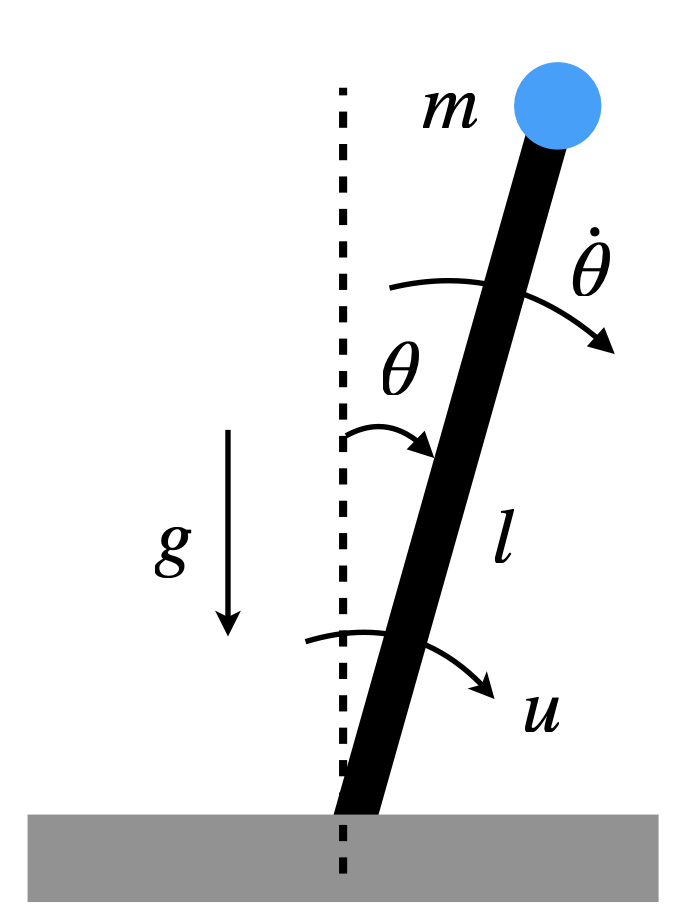
\includegraphics[width=0.4\linewidth]{images/MDP/pendulum-drawing} 

}

\caption{Inverted Pendulum.}\label{fig:mdp-pendulum-illustration}
\end{figure}

We consider the inverted pendulum with state \(s=(\theta, \dot\theta)\) and action (torque) \(a = u\), as visualized in Fig. \ref{fig:mdp-pendulum-illustration}. Our goal is to swing up the pendulum from any initial state to the upright position \(s = (0,0)\).

\textbf{Continuous-Time Dynamics}. The continuous-time dynamics of the inverted pendulum is
\[
\ddot{\theta} \;=\; \frac{g}{l}\sin(\theta) \;+\; \frac{1}{ml^2}u \;-\; c\,\dot{\theta},
\]
where \(m > 0\) is the mass of the pendulum, \(l > 0\) is the length of the pole, \(c > 0\) is the damping coefficient, and \(g\) is the gravitational constant.

\textbf{Discretization (Euler)}. With timestep \(\Delta t\), we obtain the following discrete-time dynamics:
\begin{equation}
\begin{split}
\theta_{k+1} &= \theta_k + \Delta t \, \dot{\theta}_k, \\
\dot{\theta}_{k+1} &= \dot{\theta}_k + \Delta t
\Big(\tfrac{g}{l}\sin(\theta_k) + \tfrac{1}{ml^2}u_k - c\,\dot{\theta}_k\Big).
\end{split}
\label{eq:PendulumDynamicsDiscrete}
\end{equation}

We wrap angles to \([-\pi,\pi]\) via \(\operatorname{wrap}(\theta)=\mathrm{atan2}(\sin\theta,\cos\theta)\).

\textbf{Tabular MDP}. We convert the discrete-time dynamics into a tabular MDP.

\begin{itemize}
\tightlist
\item
  \textbf{State grid.} \(\theta \in [-\pi,\pi]\), \(\dot\theta \in [-\pi,\pi]\) on uniform grids:
  \[
  \mathcal{S}=\{\;(\theta_i,\dot\theta_j)\;:\; i=1,\dots,N_\theta,\; j=1, \dots, N_{\dot\theta}\;\}.
  \]
\item
  \textbf{Action grid.} \(u \in [-mgl/2, mgl/2]\) on \(N_u\) uniform points:
  \[
  \mathcal{A}=\{u_\ell:\ell=1,\dots,N_u\}.
  \]
\item
  \textbf{Stochastic transition kernel (nearest-3 interpolation).} From a grid point \(s=(\theta_i,\dot\theta_j)\) and an action \(u_\ell\),
  compute the next continuous state \(s^+ = (\theta^+,\dot\theta^+)\) via the discrete-time dynamics in \eqref{eq:PendulumDynamicsDiscrete}.
  If \(s^+\notin\mathcal{S}\), choose the three closest grid states
  \(\{s^{(1)},s^{(2)},s^{(3)}\}\) by Euclidean distance in \((\theta,\dot\theta)\) and assign
  probabilities
  \[
  p_r \propto \frac{1}{\|s^+ - s^{(r)}\|_2 + \varepsilon},\quad r=1,2,3,
  \qquad \sum_r p_r=1,
  \]
  so nearer grid points receive higher probability (use a small \(\varepsilon>0\) to avoid division by zero).
\item
  \textbf{Reward.} A quadratic shaping penalty around the upright equilibrium:
  \[
  R(s,a) = -\Big(\theta^2 + 0.1\,\dot\theta^2 + 0.01\,u^2\Big).
  \]
\item
  \textbf{Discount.} \(\gamma \in [0,1)\). We obtain a discounted, infinite-horizon, \textbf{tabular} MDP.
\end{itemize}

\textbf{Policy}. For policy evaluation, consider \(\pi(a\mid s)\) be uniform over the discretized actions, i.e., a random policy.

\textbf{Policy Evaluation}. The following python script performs policy evaluation.

\begin{Shaded}
\begin{Highlighting}[]
\ImportTok{import}\NormalTok{ numpy }\ImportTok{as}\NormalTok{ np}
\ImportTok{import}\NormalTok{ matplotlib.pyplot }\ImportTok{as}\NormalTok{ plt}

\CommentTok{\# {-}{-}{-}{-}{-} Physical \& MDP parameters {-}{-}{-}{-}{-}}
\NormalTok{g, l, m, c }\OperatorTok{=} \FloatTok{9.81}\NormalTok{, }\FloatTok{1.0}\NormalTok{, }\FloatTok{1.0}\NormalTok{, }\FloatTok{0.1}
\NormalTok{dt }\OperatorTok{=} \FloatTok{0.05}
\NormalTok{gamma }\OperatorTok{=} \FloatTok{0.97}
\NormalTok{eps }\OperatorTok{=} \FloatTok{1e{-}8}

\CommentTok{\# Grids}
\NormalTok{N\_theta }\OperatorTok{=} \DecValTok{41}
\NormalTok{N\_thetadot }\OperatorTok{=} \DecValTok{41}
\NormalTok{N\_u }\OperatorTok{=} \DecValTok{21}

\NormalTok{theta\_grid }\OperatorTok{=}\NormalTok{ np.linspace(}\OperatorTok{{-}}\NormalTok{np.pi, np.pi, N\_theta)}
\NormalTok{thetadot\_grid }\OperatorTok{=}\NormalTok{ np.linspace(}\OperatorTok{{-}}\NormalTok{np.pi, np.pi, N\_thetadot)}
\NormalTok{u\_max }\OperatorTok{=} \FloatTok{0.5} \OperatorTok{*}\NormalTok{ m }\OperatorTok{*}\NormalTok{ g }\OperatorTok{*}\NormalTok{ l}
\NormalTok{u\_grid }\OperatorTok{=}\NormalTok{ np.linspace(}\OperatorTok{{-}}\NormalTok{u\_max, u\_max, N\_u)}

\CommentTok{\# Helpers to index/unwrap}
\KeywordTok{def}\NormalTok{ wrap\_angle(x):}
    \ControlFlowTok{return}\NormalTok{ np.arctan2(np.sin(x), np.cos(x))}

\KeywordTok{def}\NormalTok{ state\_index(i, j):}
    \ControlFlowTok{return}\NormalTok{ i }\OperatorTok{*}\NormalTok{ N\_thetadot }\OperatorTok{+}\NormalTok{ j}

\KeywordTok{def}\NormalTok{ index\_to\_state(idx):}
\NormalTok{    i }\OperatorTok{=}\NormalTok{ idx }\OperatorTok{//}\NormalTok{ N\_thetadot}
\NormalTok{    j }\OperatorTok{=}\NormalTok{ idx }\OperatorTok{\%}\NormalTok{ N\_thetadot}
    \ControlFlowTok{return}\NormalTok{ theta\_grid[i], thetadot\_grid[j]}

\NormalTok{S }\OperatorTok{=}\NormalTok{ N\_theta }\OperatorTok{*}\NormalTok{ N\_thetadot}
\NormalTok{A }\OperatorTok{=}\NormalTok{ N\_u}

\CommentTok{\# {-}{-}{-}{-}{-} Dynamics step (continuous {-}\textgreater{} one Euler step) {-}{-}{-}{-}{-}}
\KeywordTok{def}\NormalTok{ step\_euler(theta, thetadot, u):}
\NormalTok{    theta\_next }\OperatorTok{=}\NormalTok{ wrap\_angle(theta }\OperatorTok{+}\NormalTok{ dt }\OperatorTok{*}\NormalTok{ thetadot)}
\NormalTok{    thetadot\_next }\OperatorTok{=}\NormalTok{ thetadot }\OperatorTok{+}\NormalTok{ dt }\OperatorTok{*}\NormalTok{ ((g}\OperatorTok{/}\NormalTok{l) }\OperatorTok{*}\NormalTok{ np.sin(theta) }\OperatorTok{+}\NormalTok{ (}\DecValTok{1}\OperatorTok{/}\NormalTok{(m}\OperatorTok{*}\NormalTok{l}\OperatorTok{*}\NormalTok{l))}\OperatorTok{*}\NormalTok{u }\OperatorTok{{-}}\NormalTok{ c}\OperatorTok{*}\NormalTok{thetadot)}
    \CommentTok{\# clip angular velocity to grid range (bounded MDP)}
\NormalTok{    thetadot\_next }\OperatorTok{=}\NormalTok{ np.clip(thetadot\_next, thetadot\_grid[}\DecValTok{0}\NormalTok{], thetadot\_grid[}\OperatorTok{{-}}\DecValTok{1}\NormalTok{])}
    \ControlFlowTok{return}\NormalTok{ theta\_next, thetadot\_next}

\CommentTok{\# {-}{-}{-}{-}{-} Find 3 nearest grid states and probability weights (inverse{-}distance) {-}{-}{-}{-}{-}}
\CommentTok{\# Pre{-}compute all grid points for fast nearest neighbor search}
\NormalTok{grid\_pts }\OperatorTok{=}\NormalTok{ np.stack(np.meshgrid(theta\_grid, thetadot\_grid, indexing}\OperatorTok{=}\StringTok{\textquotesingle{}ij\textquotesingle{}}\NormalTok{), axis}\OperatorTok{={-}}\DecValTok{1}\NormalTok{).reshape(}\OperatorTok{{-}}\DecValTok{1}\NormalTok{, }\DecValTok{2}\NormalTok{)}

\KeywordTok{def}\NormalTok{ nearest3\_probs(theta\_next, thetadot\_next):}
\NormalTok{    x }\OperatorTok{=}\NormalTok{ np.array([theta\_next, thetadot\_next])}
\NormalTok{    dists }\OperatorTok{=}\NormalTok{ np.linalg.norm(grid\_pts }\OperatorTok{{-}}\NormalTok{ x[}\VariableTok{None}\NormalTok{, :], axis}\OperatorTok{=}\DecValTok{1}\NormalTok{)}
\NormalTok{    nn\_idx }\OperatorTok{=}\NormalTok{ np.argpartition(dists, }\DecValTok{3}\NormalTok{)[:}\DecValTok{3}\NormalTok{]  }\CommentTok{\# three smallest (unordered)}
    \CommentTok{\# sort those 3 by distance for stability}
\NormalTok{    nn\_idx }\OperatorTok{=}\NormalTok{ nn\_idx[np.argsort(dists[nn\_idx])]}
\NormalTok{    d }\OperatorTok{=}\NormalTok{ dists[nn\_idx]}
\NormalTok{    w }\OperatorTok{=} \FloatTok{1.0} \OperatorTok{/}\NormalTok{ (d }\OperatorTok{+}\NormalTok{ eps)}
\NormalTok{    p }\OperatorTok{=}\NormalTok{ w }\OperatorTok{/}\NormalTok{ w.}\BuiltInTok{sum}\NormalTok{()}
    \ControlFlowTok{return}\NormalTok{ nn\_idx.astype(}\BuiltInTok{int}\NormalTok{), p}

\CommentTok{\# {-}{-}{-}{-}{-} Reward {-}{-}{-}{-}{-}}
\KeywordTok{def}\NormalTok{ reward(theta, thetadot, u):}
    \ControlFlowTok{return} \OperatorTok{{-}}\NormalTok{(theta}\OperatorTok{**}\DecValTok{2} \OperatorTok{+} \FloatTok{0.1}\OperatorTok{*}\NormalTok{thetadot}\OperatorTok{**}\DecValTok{2} \OperatorTok{+} \FloatTok{0.01}\OperatorTok{*}\NormalTok{u}\OperatorTok{**}\DecValTok{2}\NormalTok{)}

\CommentTok{\# {-}{-}{-}{-}{-} Build tabular MDP: R[s,a] and sparse P[s,a,3] {-}{-}{-}{-}{-}}
\NormalTok{R }\OperatorTok{=}\NormalTok{ np.zeros((S, A))}
\NormalTok{NS\_idx }\OperatorTok{=}\NormalTok{ np.zeros((S, A, }\DecValTok{3}\NormalTok{), dtype}\OperatorTok{=}\BuiltInTok{int}\NormalTok{)   }\CommentTok{\# next{-}state indices (3 nearest)}
\NormalTok{NS\_prob }\OperatorTok{=}\NormalTok{ np.zeros((S, A, }\DecValTok{3}\NormalTok{))            }\CommentTok{\# their probabilities}

\ControlFlowTok{for}\NormalTok{ i, th }\KeywordTok{in} \BuiltInTok{enumerate}\NormalTok{(theta\_grid):}
    \ControlFlowTok{for}\NormalTok{ j, thd }\KeywordTok{in} \BuiltInTok{enumerate}\NormalTok{(thetadot\_grid):}
\NormalTok{        s }\OperatorTok{=}\NormalTok{ state\_index(i, j)}
        \ControlFlowTok{for}\NormalTok{ a, u }\KeywordTok{in} \BuiltInTok{enumerate}\NormalTok{(u\_grid):}
            \CommentTok{\# reward at current (s,a)}
\NormalTok{            R[s, a] }\OperatorTok{=}\NormalTok{ reward(th, thd, u)}
            \CommentTok{\# next continuous state}
\NormalTok{            th\_n, thd\_n }\OperatorTok{=}\NormalTok{ step\_euler(th, thd, u)}
            \CommentTok{\# map to 3 nearest grid states}
\NormalTok{            nn\_idx, p }\OperatorTok{=}\NormalTok{ nearest3\_probs(th\_n, thd\_n)}
\NormalTok{            NS\_idx[s, a, :] }\OperatorTok{=}\NormalTok{ nn\_idx}
\NormalTok{            NS\_prob[s, a, :] }\OperatorTok{=}\NormalTok{ p}

\CommentTok{\# {-}{-}{-}{-}{-} Fixed policy: uniform over actions {-}{-}{-}{-}{-}}
\NormalTok{Pi }\OperatorTok{=}\NormalTok{ np.full((S, A), }\FloatTok{1.0} \OperatorTok{/}\NormalTok{ A)}

\CommentTok{\# {-}{-}{-}{-}{-} Iterative policy evaluation {-}{-}{-}{-}{-}}
\NormalTok{V }\OperatorTok{=}\NormalTok{ np.zeros(S)  }\CommentTok{\# initialization (any vector works)}
\NormalTok{tol }\OperatorTok{=} \FloatTok{1e{-}6}
\NormalTok{max\_iters }\OperatorTok{=} \DecValTok{10000}

\ControlFlowTok{for}\NormalTok{ k }\KeywordTok{in} \BuiltInTok{range}\NormalTok{(max\_iters):}
\NormalTok{    V\_new }\OperatorTok{=}\NormalTok{ np.zeros\_like(V)}
    \CommentTok{\# Compute Bellman update: V\_\{k+1\}(s) = sum\_a Pi(s,a)[ R(s,a) + gamma * sum\_j P(s,a,j) V\_k(ns\_j) ]}
    \CommentTok{\# First, expected next V for each (s,a)}
\NormalTok{    EV\_next }\OperatorTok{=}\NormalTok{ (NS\_prob }\OperatorTok{*}\NormalTok{ V[NS\_idx]).}\BuiltInTok{sum}\NormalTok{(axis}\OperatorTok{=}\DecValTok{2}\NormalTok{)  }\CommentTok{\# shape: (S, A)}
    \CommentTok{\# Then expectation over actions under Pi}
\NormalTok{    V\_new }\OperatorTok{=}\NormalTok{ (Pi }\OperatorTok{*}\NormalTok{ (R }\OperatorTok{+}\NormalTok{ gamma }\OperatorTok{*}\NormalTok{ EV\_next)).}\BuiltInTok{sum}\NormalTok{(axis}\OperatorTok{=}\DecValTok{1}\NormalTok{)  }\CommentTok{\# shape: (S,)}
    \CommentTok{\# Check convergence}
    \ControlFlowTok{if}\NormalTok{ np.}\BuiltInTok{max}\NormalTok{(np.}\BuiltInTok{abs}\NormalTok{(V\_new }\OperatorTok{{-}}\NormalTok{ V)) }\OperatorTok{\textless{}}\NormalTok{ tol:}
\NormalTok{        V }\OperatorTok{=}\NormalTok{ V\_new}
        \BuiltInTok{print}\NormalTok{(}\SpecialStringTok{f"Converged in }\SpecialCharTok{\{}\NormalTok{k}\OperatorTok{+}\DecValTok{1}\SpecialCharTok{\}}\SpecialStringTok{ iterations (sup{-}norm change \textless{} }\SpecialCharTok{\{}\NormalTok{tol}\SpecialCharTok{\}}\SpecialStringTok{)."}\NormalTok{)}
        \ControlFlowTok{break}
\NormalTok{    V }\OperatorTok{=}\NormalTok{ V\_new}
\ControlFlowTok{else}\NormalTok{:}
    \BuiltInTok{print}\NormalTok{(}\SpecialStringTok{f"Reached max\_iters=}\SpecialCharTok{\{}\NormalTok{max\_iters}\SpecialCharTok{\}}\SpecialStringTok{ without meeting tolerance }\SpecialCharTok{\{}\NormalTok{tol}\SpecialCharTok{\}}\SpecialStringTok{."}\NormalTok{)}

\NormalTok{V\_grid }\OperatorTok{=}\NormalTok{ V.reshape(N\_theta, N\_thetadot)}

\CommentTok{\# V\_grid: shape (N\_theta, N\_thetadot)}
\CommentTok{\# theta\_grid, thetadot\_grid already defined}
\NormalTok{fig, ax }\OperatorTok{=}\NormalTok{ plt.subplots(figsize}\OperatorTok{=}\NormalTok{(}\DecValTok{7}\NormalTok{,}\DecValTok{5}\NormalTok{), dpi}\OperatorTok{=}\DecValTok{120}\NormalTok{)}
\NormalTok{im }\OperatorTok{=}\NormalTok{ ax.imshow(}
\NormalTok{    V\_grid,}
\NormalTok{    origin}\OperatorTok{=}\StringTok{"lower"}\NormalTok{,}
\NormalTok{    extent}\OperatorTok{=}\NormalTok{[thetadot\_grid.}\BuiltInTok{min}\NormalTok{(), thetadot\_grid.}\BuiltInTok{max}\NormalTok{(),}
\NormalTok{            theta\_grid.}\BuiltInTok{min}\NormalTok{(), theta\_grid.}\BuiltInTok{max}\NormalTok{()],}
\NormalTok{    aspect}\OperatorTok{=}\StringTok{"auto"}\NormalTok{,}
\NormalTok{    cmap}\OperatorTok{=}\StringTok{"viridis"}  \CommentTok{\# any matplotlib colormap, e.g., "plasma", "inferno"}
\NormalTok{)}
\NormalTok{cbar }\OperatorTok{=}\NormalTok{ fig.colorbar(im, ax}\OperatorTok{=}\NormalTok{ax)}
\NormalTok{cbar.set\_label(}\VerbatimStringTok{r"$V\^{}\textbackslash{}pi(\textbackslash{}theta,\textbackslash{}dot\{\textbackslash{}theta\})$"}\NormalTok{)}

\NormalTok{ax.set\_xlabel(}\VerbatimStringTok{r"$\textbackslash{}dot\{\textbackslash{}theta\}$"}\NormalTok{)}
\NormalTok{ax.set\_ylabel(}\VerbatimStringTok{r"$\textbackslash{}theta$"}\NormalTok{)}
\NormalTok{ax.set\_title(}\VerbatimStringTok{r"State{-}value $V\^{}\textbackslash{}pi$ (tabular policy evaluation)"}\NormalTok{)}

\NormalTok{plt.tight\_layout()}
\NormalTok{plt.show()}
\end{Highlighting}
\end{Shaded}

Running the code, it shows that policy evaluation converges in 518 iterations under tolerance \(10^{-6}\).

Fig. \ref{fig:mdp-pendulum-value-function-policy-evaluation} plots the value function over the state grid.

\begin{figure}

{\centering 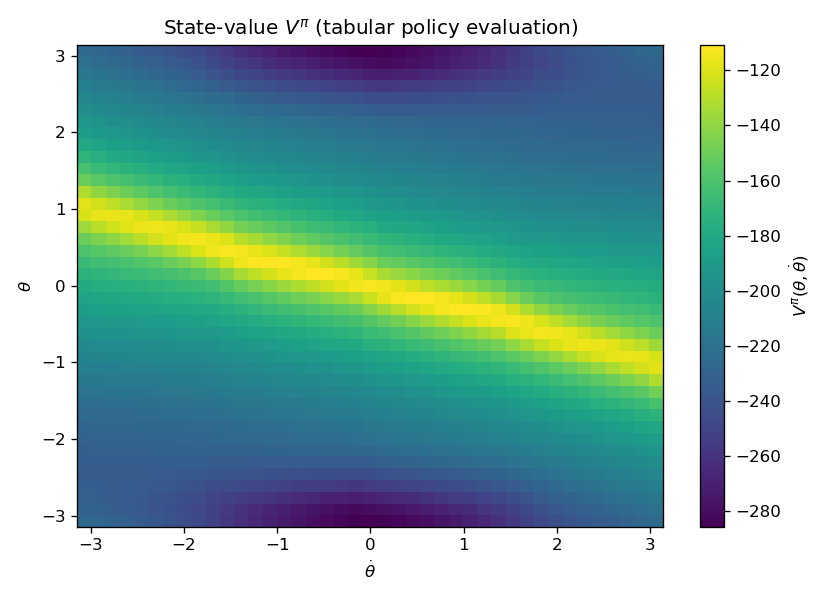
\includegraphics[width=0.8\linewidth]{images/MDP/pendulum_policy_evaluation} 

}

\caption{Value Function from Policy Evaluation.}\label{fig:mdp-pendulum-value-function-policy-evaluation}
\end{figure}

You can play with the code \href{https://github.com/ComputationalRobotics/2025-ES-AM-158-LECTURE-CODE/blob/main/pendulum_policy_evaluation.py}{here}.

\end{example}

\subsection{Principle of Optimality}\label{principle-of-optimality}

In an infinite-horizon MDP, our goal is to find the optimal policy that maximizes the expected long-term discounted return:
\[
V^\star := \max_{\pi} \mathbb{E}_{s \sim \mu(\cdot)} [V^\pi(s)],
\]
where \(\mu\) is a given initial distribution. We call \(V^\star\) the optimal value function.

Given a policy \(\pi\) and its associated value function \(V^\pi\), how do we know if the policy is already optimal?

\begin{theorem}[Bellman Optimality (Infinite Horizon)]
\protect\hypertarget{thm:BellmanOptimalityInfiniteHorizon}{}\label{thm:BellmanOptimalityInfiniteHorizon}For an infinite-horizon MDP with discount factor \(\gamma \in [0,1)\),
the optimal state-value function \(V^\star(s)\)
satisfies the Bellman optimality equation
\begin{equation}
V^\star(s) \;=\; \max_{a \in \mathcal{A}}
\Big[\, R(s,a) + \gamma \sum_{s' \in \mathcal{S}} P(s' \mid s,a)\, V^\star(s') \,\Big].
\label{eq:BellmanOptimalityInfiniteHorizonStateValue}
\end{equation}

Define the optimal action-value function as
\begin{equation}
Q^\star(s,a) = R(s,a) + \gamma \sum_{s' \in \mathcal{S}} P(s' \mid s, a) V^\star(s').
\label{eq:InfiniteHorizonOptimalActionValue}
\end{equation}
We have that \(Q^\star(s,a)\) satisfies
\begin{equation}
Q^\star(s,a) \;=\; R(s,a) + \gamma \sum_{s' \in \mathcal{S}} P(s' \mid s,a)\, \left[\max_{a' \in \mathcal{A}} Q^\star(s',a') \right].
\label{eq:BellmanOptimalityInfiniteHorizonActionValue}
\end{equation}

Moreover, any greedy policy with respect to \(V^\star\) (equivalently, to \(Q^\star\)) is optimal:
\begin{equation}
\begin{split}
\pi^\star(s) & \in \arg\max_{a \in \mathcal{A}}
\Big[\, R(s,a) + \gamma \sum_{s'} P(s' \mid s,a)\, V^\star(s') \,\Big]
\quad\Longleftrightarrow\quad \\
\pi^\star(s) & \in \arg\max_{a \in \mathcal{A}} Q^\star(s,a).
\end{split}
\label{eq:InfiniteHorizonOptimalPolicy}
\end{equation}
\end{theorem}

\begin{proof}
We will first show that \(V^\star\) has statewise dominance over all other policies, and then show that \(V^\star\) can be attained by the greedy policy.

\textbf{Claim.} For any discounted MDP with \(\gamma \in [0,1)\) and any policy \(\pi\),
\[
V^\star(s) \;\ge\; V^{\pi}(s)\qquad \forall s\in\mathcal{S},
\]
where \(V^\star\) is the unique solution of the Bellman \textbf{optimality} equation and \(V^\pi\) solves the Bellman \textbf{consistency} equation for \(\pi\).

\textbf{Proof via Bellman Operators}.
Define the Bellman operators
\[
(T^\pi V)(s) := \sum_{a}\pi(a\mid s)\Big[ R(s,a)+\gamma \sum_{s'} P(s'\mid s,a)V(s') \Big],
\]
\[
(T^\star V)(s) := \max_{a}\Big[ R(s,a)+\gamma \sum_{s'} P(s'\mid s,a)V(s') \Big].
\]

Key facts:

\begin{enumerate}
\def\labelenumi{\arabic{enumi}.}
\tightlist
\item
  (\textbf{Monotonicity}) If \(V \ge W\) componentwise, then \(T^\pi V \ge T^\pi W\) and \(T^\star V \ge T^\star W\).
\item
  (\textbf{Dominance of \(T^*\)}) For any \(V\) and any \(\pi\),
  \[
  T^\star V \;\ge\; T^\pi V
  \]
  because the max over actions is at least the \(\pi\)-weighted average.
\item
  (\textbf{Fixed points}) \(V^\pi = T^\pi V^\pi\) and \(V^\star = T^\star V^\star\).
\item
  (\textbf{Contraction}) Each \(T^\pi\) and \(T^\star\) is a \(\gamma\)-contraction in the sup-norm; hence their fixed points are unique.
\end{enumerate}

Now start from \(V^\pi\). Using (2),
\[
V^\pi = T^\pi V^\pi \;\le\; T^\star V^\pi.
\]
Applying \(T^\star\) repeatedly and using (1),
\[
V^\pi \;\le\; T^\star V^\pi \;\le\; (T^\star)^2 V^\pi \;\le\; \cdots
\]
The sequence \((T^\star)^k V^\pi\) converges (by contraction) to the unique fixed point of \(T^\star\), namely \(V^\star\). Taking limits preserves the inequality, yielding \(V^\pi \le V^\star\) statewise.
\end{proof}

The Bellman optimality condition tells us, if a policy \(\pi\) is already greedy with respect to its value function \(V^\pi\), then \(\pi\) is the optimal policy and \(V^\pi\) is the optimal value function.

In the next, we introduce two algorithms that can guarantee finding the optimal policy and the optimal value function.

The first algorithm, policy iteration (PI), iterates over the space of policies; while the second algorithm, value iteration (VI), iterates over the space of value functions.

\subsection{Policy Improvement}\label{policy-improvement}

The policy evaluation algorithm enables us to compute the value functions associated with a given policy \(\pi\). The next result, known as the \emph{Policy Improvement Lemma}, shows that once we have \(V^{\pi}\), constructing a greedy policy with respect to \(V^{\pi}\) guarantees performance that is at least as good as \(\pi\), and strictly better in some states unless \(\pi\) is already greedy with respect to \(V^{\pi}\).

\begin{lemma}[Policy Improvement]
\protect\hypertarget{lem:InfiniteHorizonPolicyImprovement}{}\label{lem:InfiniteHorizonPolicyImprovement}Let \(\pi\) be any policy and let \(V^{\pi}\) be its state-value function.\\
Define a new policy \(\pi'\) such that for each state \(s\),
\[
\pi'(s) \in \arg\max_{a \in \mathcal{A}}
\Big[ R(s,a) + \gamma \sum_{s'} P(s' \mid s,a) V^{\pi}(s') \Big].
\]

Then for all states \(s \in \mathcal{S}\),
\[
V^{\pi'}(s) \;\ge\; V^{\pi}(s).
\]
Moreover, the inequality is strict for some state \(s\) unless \(\pi\) is already greedy with respect to \(V^\pi\) (which implies optimality).
\end{lemma}

\begin{proof}
Let \(V^{\pi}\) be the value function of a policy \(\pi\), and define a new (possibly stochastic) policy \(\pi'\) that is greedy w.r.t. \(V^{\pi}\):
\[
\pi'(\cdot \mid s) \in \arg\max_{\mu \in \Delta(\mathcal{A})}
\sum_{a}\mu(a)\Big[ R(s,a) + \gamma \sum_{s'} P(s'\mid s,a)\, V^{\pi}(s')\Big].
\]
Define the Bellman operators
\begin{align*}
(T^{\pi}V)(s) & := \sum_a \pi(a\mid s)\Big[R(s,a)+\gamma\sum_{s'}P(s'\mid s,a)V(s')\Big],\\
(T^{\pi'}V)(s) & := \sum_a \pi'(a\mid s)\Big[\cdots\Big].
\end{align*}

\textbf{Step 1: One-step improvement at \(V^{\pi}\)}.
By greediness of \(\pi'\) w.r.t. \(V^{\pi}\),
\[
(T^{\pi'} V^{\pi})(s)
= \max_{\mu}\sum_a \mu(a)\Big[R(s,a)+\gamma\sum_{s'}P(s'\mid s,a)V^{\pi}(s')\Big]
\;\;\ge\;\; (T^{\pi} V^{\pi})(s) = V^{\pi}(s),
\]
for all \(s\). Hence
\begin{equation}
T^{\pi'} V^{\pi} \;\ge\; V^{\pi}\quad\text{(componentwise).}
\label{eq:ProofPolicyImprovementStepOne}
\end{equation}

\textbf{Step 2: Monotonicity + contraction yield global improvement}.
The operator \(T^{\pi'}\) is \textbf{monotone} (order-preserving) and a \textbf{\(\gamma\)-contraction} in the sup-norm.\\
Apply \(T^{\pi'}\) repeatedly to both sides of \eqref{eq:ProofPolicyImprovementStepOne}:
\[
(T^{\pi'})^k V^{\pi} \;\ge\; (T^{\pi'})^{k-1} V^{\pi} \;\ge\; \cdots \;\ge\; V^{\pi},\qquad k=1,2,\dots
\]
By contraction, \((T^{\pi'})^k V^{\pi} \to V^{\pi'}\), the unique fixed point of \(T^{\pi'}\).\\
Taking limits preserves the inequality, so
\[
V^{\pi'} \;\ge\; V^{\pi}\quad\text{statewise.}
\]

\textbf{Strict improvement condition}.
If there exists a state \(s\) such that
\[
(T^{\pi'} V^{\pi})(s) \;>\; V^{\pi}(s),
\]
then by monotonicity we have a strict increase at that state after one iteration, and the limit remains strictly larger at that state (or at any state that can reach it with positive probability under \(\pi'\)).\\
This happens precisely when \(\pi'\) selects, with positive probability, an action \(a\) for which
\[
Q^{\pi}(s,a)=R(s,a) + \gamma \sum_{s'} P(s'\mid s,a)\, V^{\pi}(s') \;>\; V^{\pi}(s),
\]
i.e., when \(\pi\) was not already greedy (optimal) at \(s\).
\end{proof}

\subsection{Policy Iteration}\label{policy-iteration}

The policy improvement lemma and the principle of optimality, combined together, leads to the first algorithm that guarantees convergence to an optimal policy. This algorithm is called policy iteration.

\begin{theorem}[Convergence of Policy Iteration]
\protect\hypertarget{thm:PolicyIterationConvergence}{}\label{thm:PolicyIterationConvergence}

Consider a discounted MDP with finite state and action sets and \(\gamma\in[0,1)\). Let \(\{\pi_k\}_{k\ge0}\) be the sequence produced by \emph{Policy Iteration (PI)}:

\begin{enumerate}
\def\labelenumi{\arabic{enumi}.}
\tightlist
\item
  \textbf{Policy evaluation:} compute \(V^{\pi_k}\) such that \(V^{\pi_k}=T^{\pi_k}V^{\pi_k}\).
\item
  \textbf{Policy improvement:} choose \(\pi_{k+1}\) greedy w.r.t. \(V^{\pi_k}\):
  \[
  \pi_{k+1}(s) \in \arg\max_{a}\Big[ R(s,a)+\gamma\sum_{s'}P(s'|s,a)\,V^{\pi_k}(s')\Big].
  \]
\end{enumerate}

Then:

\begin{enumerate}
\def\labelenumi{\alph{enumi}.}
\item
  \(V^{\pi_{k+1}} \ge V^{\pi_k}\) componentwise, and the inequality is strict for some state unless \(\pi_{k+1}=\pi_k\).
\item
  If \(\pi_{k+1}=\pi_k\), then \(V^{\pi_k}\) satisfies the Bellman optimality equation; hence \(\pi_k\) is optimal and \(V^{\pi_k}=V^*\).
\item
  Because the number of stationary policies is finite, PI terminates in finitely many iterations at an optimal policy \(\pi^*\) with value \(V^*\).
\item
  \(\Vert V^{\pi_{k+1}} - V^\star \Vert_{\infty} \leq \gamma \Vert V^{\pi_k} -  V^\star \Vert_{\infty}\), for any \(k\) (i.e., contraction).
\end{enumerate}

\end{theorem}

\begin{proof}
By the policy improvement lemma, we have
\[
V^{\pi_{k+1}} \geq V^{\pi_k}.
\]
By monotonicity of the Bellman operator \(T^{\pi_{k+1}}\), we have
\[
V^{\pi_{k+1}} = T^{\pi_{k+1}} V^{\pi_{k+1}} \geq  T^{\pi_{k+1}} V^{\pi_k}.
\]
By definition of the Bellman optimality operator, we have
\[
T^{\pi_{k+1}} V^{\pi_k} = T^\star V^{\pi_k}.
\]
Therefore,
\[
0 \geq V^{\pi_{k+1}} - V^\star \geq T^{\pi_{k+1}} V^{\pi_k} - V^\star = T^\star V^{\pi_k} - T^\star V^\star
\]
As a result,
\[
\Vert V^{\pi_{k+1}} - V^\star \Vert_{\infty} \leq \Vert T^\star V^{\pi_k} - T^\star V^\star \Vert_{\infty} \leq \gamma \Vert V^{\pi_k} -  V^\star \Vert_{\infty}.
\]
This proves the contraction result (d).
\end{proof}

Let us apply Policy Iteration to the inverted pendulum problem.

\begin{example}[Policy Iteration for Inverted Pendulum]
\protect\hypertarget{exm:InvertedPendulumPolicyIteration}{}\label{exm:InvertedPendulumPolicyIteration}

The following code performs policy iteration for the inverted pendulum problem.

\begin{Shaded}
\begin{Highlighting}[]
\ImportTok{import}\NormalTok{ numpy }\ImportTok{as}\NormalTok{ np}
\ImportTok{import}\NormalTok{ matplotlib.pyplot }\ImportTok{as}\NormalTok{ plt}

\CommentTok{\# {-}{-}{-}{-}{-} Physical \& MDP parameters {-}{-}{-}{-}{-}}
\NormalTok{g, l, m, c }\OperatorTok{=} \FloatTok{9.81}\NormalTok{, }\FloatTok{1.0}\NormalTok{, }\FloatTok{1.0}\NormalTok{, }\FloatTok{0.1}
\NormalTok{dt }\OperatorTok{=} \FloatTok{0.05}
\NormalTok{gamma }\OperatorTok{=} \FloatTok{0.97}
\NormalTok{eps }\OperatorTok{=} \FloatTok{1e{-}8}

\CommentTok{\# Grids}
\NormalTok{N\_theta }\OperatorTok{=} \DecValTok{101}
\NormalTok{N\_thetadot }\OperatorTok{=} \DecValTok{101}
\NormalTok{N\_u }\OperatorTok{=} \DecValTok{51}

\NormalTok{theta\_grid }\OperatorTok{=}\NormalTok{ np.linspace(}\OperatorTok{{-}}\FloatTok{1.5}\OperatorTok{*}\NormalTok{np.pi, }\FloatTok{1.5}\OperatorTok{*}\NormalTok{np.pi, N\_theta)}
\NormalTok{thetadot\_grid }\OperatorTok{=}\NormalTok{ np.linspace(}\OperatorTok{{-}}\FloatTok{1.5}\OperatorTok{*}\NormalTok{np.pi, }\FloatTok{1.5}\OperatorTok{*}\NormalTok{np.pi, N\_thetadot)}
\NormalTok{u\_max }\OperatorTok{=} \FloatTok{0.5} \OperatorTok{*}\NormalTok{ m }\OperatorTok{*}\NormalTok{ g }\OperatorTok{*}\NormalTok{ l}
\NormalTok{u\_grid }\OperatorTok{=}\NormalTok{ np.linspace(}\OperatorTok{{-}}\NormalTok{u\_max, u\_max, N\_u)}

\CommentTok{\# Helpers to index/unwrap}
\KeywordTok{def}\NormalTok{ wrap\_angle(x):}
    \ControlFlowTok{return}\NormalTok{ np.arctan2(np.sin(x), np.cos(x))}

\KeywordTok{def}\NormalTok{ state\_index(i, j):}
    \ControlFlowTok{return}\NormalTok{ i }\OperatorTok{*}\NormalTok{ N\_thetadot }\OperatorTok{+}\NormalTok{ j}

\KeywordTok{def}\NormalTok{ index\_to\_state(idx):}
\NormalTok{    i }\OperatorTok{=}\NormalTok{ idx }\OperatorTok{//}\NormalTok{ N\_thetadot}
\NormalTok{    j }\OperatorTok{=}\NormalTok{ idx }\OperatorTok{\%}\NormalTok{ N\_thetadot}
    \ControlFlowTok{return}\NormalTok{ theta\_grid[i], thetadot\_grid[j]}

\NormalTok{S }\OperatorTok{=}\NormalTok{ N\_theta }\OperatorTok{*}\NormalTok{ N\_thetadot}
\NormalTok{A }\OperatorTok{=}\NormalTok{ N\_u}

\CommentTok{\# {-}{-}{-}{-}{-} Dynamics step (continuous {-}\textgreater{} one Euler step) {-}{-}{-}{-}{-}}
\KeywordTok{def}\NormalTok{ step\_euler(theta, thetadot, u):}
\NormalTok{    theta\_next }\OperatorTok{=}\NormalTok{ wrap\_angle(theta }\OperatorTok{+}\NormalTok{ dt }\OperatorTok{*}\NormalTok{ thetadot)}
\NormalTok{    thetadot\_next }\OperatorTok{=}\NormalTok{ thetadot }\OperatorTok{+}\NormalTok{ dt }\OperatorTok{*}\NormalTok{ ((g}\OperatorTok{/}\NormalTok{l) }\OperatorTok{*}\NormalTok{ np.sin(theta) }\OperatorTok{+}\NormalTok{ (}\DecValTok{1}\OperatorTok{/}\NormalTok{(m}\OperatorTok{*}\NormalTok{l}\OperatorTok{*}\NormalTok{l))}\OperatorTok{*}\NormalTok{u }\OperatorTok{{-}}\NormalTok{ c}\OperatorTok{*}\NormalTok{thetadot)}
    \CommentTok{\# clip angular velocity to grid range (bounded MDP)}
\NormalTok{    thetadot\_next }\OperatorTok{=}\NormalTok{ np.clip(thetadot\_next, thetadot\_grid[}\DecValTok{0}\NormalTok{], thetadot\_grid[}\OperatorTok{{-}}\DecValTok{1}\NormalTok{])}
    \ControlFlowTok{return}\NormalTok{ theta\_next, thetadot\_next}

\CommentTok{\# {-}{-}{-}{-}{-} Find 3 nearest grid states and probability weights (inverse{-}distance) {-}{-}{-}{-}{-}}
\NormalTok{grid\_pts }\OperatorTok{=}\NormalTok{ np.stack(np.meshgrid(theta\_grid, thetadot\_grid, indexing}\OperatorTok{=}\StringTok{\textquotesingle{}ij\textquotesingle{}}\NormalTok{), axis}\OperatorTok{={-}}\DecValTok{1}\NormalTok{).reshape(}\OperatorTok{{-}}\DecValTok{1}\NormalTok{, }\DecValTok{2}\NormalTok{)}

\KeywordTok{def}\NormalTok{ nearest3\_probs(theta\_next, thetadot\_next):}
\NormalTok{    x }\OperatorTok{=}\NormalTok{ np.array([theta\_next, thetadot\_next])}
\NormalTok{    dists }\OperatorTok{=}\NormalTok{ np.linalg.norm(grid\_pts }\OperatorTok{{-}}\NormalTok{ x[}\VariableTok{None}\NormalTok{, :], axis}\OperatorTok{=}\DecValTok{1}\NormalTok{)}
\NormalTok{    nn\_idx }\OperatorTok{=}\NormalTok{ np.argpartition(dists, }\DecValTok{3}\NormalTok{)[:}\DecValTok{3}\NormalTok{]      }\CommentTok{\# three smallest (unordered)}
\NormalTok{    nn\_idx }\OperatorTok{=}\NormalTok{ nn\_idx[np.argsort(dists[nn\_idx])]  }\CommentTok{\# sort those 3 by distance}
\NormalTok{    d }\OperatorTok{=}\NormalTok{ dists[nn\_idx]}
\NormalTok{    w }\OperatorTok{=} \FloatTok{1.0} \OperatorTok{/}\NormalTok{ (d }\OperatorTok{+}\NormalTok{ eps)}
\NormalTok{    p }\OperatorTok{=}\NormalTok{ w }\OperatorTok{/}\NormalTok{ w.}\BuiltInTok{sum}\NormalTok{()}
    \ControlFlowTok{return}\NormalTok{ nn\_idx.astype(}\BuiltInTok{int}\NormalTok{), p}

\CommentTok{\# {-}{-}{-}{-}{-} Reward {-}{-}{-}{-}{-}}
\KeywordTok{def}\NormalTok{ reward(theta, thetadot, u):}
    \ControlFlowTok{return} \OperatorTok{{-}}\NormalTok{(theta}\OperatorTok{**}\DecValTok{2} \OperatorTok{+} \FloatTok{0.1}\OperatorTok{*}\NormalTok{thetadot}\OperatorTok{**}\DecValTok{2} \OperatorTok{+} \FloatTok{0.01}\OperatorTok{*}\NormalTok{u}\OperatorTok{**}\DecValTok{2}\NormalTok{)}

\CommentTok{\# {-}{-}{-}{-}{-} Build tabular MDP: R[s,a] and sparse P[s,a,3] {-}{-}{-}{-}{-}}
\NormalTok{R }\OperatorTok{=}\NormalTok{ np.zeros((S, A))}
\NormalTok{NS\_idx }\OperatorTok{=}\NormalTok{ np.zeros((S, A, }\DecValTok{3}\NormalTok{), dtype}\OperatorTok{=}\BuiltInTok{int}\NormalTok{)   }\CommentTok{\# next{-}state indices (3 nearest)}
\NormalTok{NS\_prob }\OperatorTok{=}\NormalTok{ np.zeros((S, A, }\DecValTok{3}\NormalTok{))             }\CommentTok{\# their probabilities}

\ControlFlowTok{for}\NormalTok{ i, th }\KeywordTok{in} \BuiltInTok{enumerate}\NormalTok{(theta\_grid):}
    \ControlFlowTok{for}\NormalTok{ j, thd }\KeywordTok{in} \BuiltInTok{enumerate}\NormalTok{(thetadot\_grid):}
\NormalTok{        s }\OperatorTok{=}\NormalTok{ state\_index(i, j)}
        \ControlFlowTok{for}\NormalTok{ a, u }\KeywordTok{in} \BuiltInTok{enumerate}\NormalTok{(u\_grid):}
            \CommentTok{\# reward at current (s,a)}
\NormalTok{            R[s, a] }\OperatorTok{=}\NormalTok{ reward(th, thd, u)}
            \CommentTok{\# next continuous state}
\NormalTok{            th\_n, thd\_n }\OperatorTok{=}\NormalTok{ step\_euler(th, thd, u)}
            \CommentTok{\# map to 3 nearest grid states}
\NormalTok{            nn\_idx, p }\OperatorTok{=}\NormalTok{ nearest3\_probs(th\_n, thd\_n)}
\NormalTok{            NS\_idx[s, a, :] }\OperatorTok{=}\NormalTok{ nn\_idx}
\NormalTok{            NS\_prob[s, a, :] }\OperatorTok{=}\NormalTok{ p}

\CommentTok{\# =======================}
\CommentTok{\#     POLICY ITERATION}
\CommentTok{\# =======================}

\CommentTok{\# Represent policy as a deterministic action index per state: pi[s] in \{0..A{-}1\}}
\CommentTok{\# Start from uniform{-}random policy (deterministic tie{-}breaker: middle action)}
\NormalTok{pi }\OperatorTok{=}\NormalTok{ np.full(S, A }\OperatorTok{//} \DecValTok{2}\NormalTok{, dtype}\OperatorTok{=}\BuiltInTok{int}\NormalTok{)}

\KeywordTok{def}\NormalTok{ policy\_evaluation(pi, V\_init}\OperatorTok{=}\VariableTok{None}\NormalTok{, tol}\OperatorTok{=}\FloatTok{1e{-}6}\NormalTok{, max\_iters}\OperatorTok{=}\DecValTok{10000}\NormalTok{):}
    \CommentTok{"""Iterative policy evaluation for deterministic pi (action index per state)."""}
\NormalTok{    V }\OperatorTok{=}\NormalTok{ np.zeros(S) }\ControlFlowTok{if}\NormalTok{ V\_init }\KeywordTok{is} \VariableTok{None} \ControlFlowTok{else}\NormalTok{ V\_init.copy()}
    \ControlFlowTok{for}\NormalTok{ k }\KeywordTok{in} \BuiltInTok{range}\NormalTok{(max\_iters):}
        \CommentTok{\# For each state s, use chosen action a = pi[s]}
\NormalTok{        a }\OperatorTok{=}\NormalTok{ pi  }\CommentTok{\# shape (S,)}
        \CommentTok{\# Expected next value under chosen action}
\NormalTok{        EV\_next }\OperatorTok{=}\NormalTok{ (NS\_prob[np.arange(S), a] }\OperatorTok{*}\NormalTok{ V[NS\_idx[np.arange(S), a]]).}\BuiltInTok{sum}\NormalTok{(axis}\OperatorTok{=}\DecValTok{1}\NormalTok{)  }\CommentTok{\# (S,)}
\NormalTok{        V\_new }\OperatorTok{=}\NormalTok{ R[np.arange(S), a] }\OperatorTok{+}\NormalTok{ gamma }\OperatorTok{*}\NormalTok{ EV\_next}
        \ControlFlowTok{if}\NormalTok{ np.}\BuiltInTok{max}\NormalTok{(np.}\BuiltInTok{abs}\NormalTok{(V\_new }\OperatorTok{{-}}\NormalTok{ V)) }\OperatorTok{\textless{}}\NormalTok{ tol:}
            \CommentTok{\# print(f"Policy evaluation converged in \{k+1\} iterations.")}
            \ControlFlowTok{return}\NormalTok{ V\_new}
\NormalTok{        V }\OperatorTok{=}\NormalTok{ V\_new}
    \CommentTok{\# print("Policy evaluation reached max\_iters without meeting tolerance.")}
    \ControlFlowTok{return}\NormalTok{ V}

\KeywordTok{def}\NormalTok{ policy\_improvement(V, pi\_old}\OperatorTok{=}\VariableTok{None}\NormalTok{):}
    \CommentTok{"""Greedy improvement: pi\textquotesingle{}(s) = argmax\_a [ R(s,a) + gamma * E[V(s\textquotesingle{})] ]."""}
    \CommentTok{\# Compute Q(s,a) = R + gamma * sum\_j P(s,a,j) V(ns\_j)}
\NormalTok{    EV\_next }\OperatorTok{=}\NormalTok{ (NS\_prob }\OperatorTok{*}\NormalTok{ V[NS\_idx]).}\BuiltInTok{sum}\NormalTok{(axis}\OperatorTok{=}\DecValTok{2}\NormalTok{)      }\CommentTok{\# (S, A)}
\NormalTok{    Q }\OperatorTok{=}\NormalTok{ R }\OperatorTok{+}\NormalTok{ gamma }\OperatorTok{*}\NormalTok{ EV\_next                           }\CommentTok{\# (S, A)}
\NormalTok{    pi\_new }\OperatorTok{=}\NormalTok{ np.argmax(Q, axis}\OperatorTok{=}\DecValTok{1}\NormalTok{).astype(}\BuiltInTok{int}\NormalTok{)         }\CommentTok{\# greedy deterministic policy}
\NormalTok{    stable }\OperatorTok{=}\NormalTok{ (pi\_old }\KeywordTok{is} \KeywordTok{not} \VariableTok{None}\NormalTok{) }\KeywordTok{and}\NormalTok{ np.array\_equal(pi\_new, pi\_old)}
    \ControlFlowTok{return}\NormalTok{ pi\_new, stable}

\CommentTok{\# Main PI loop}
\NormalTok{max\_pi\_iters }\OperatorTok{=} \DecValTok{100}
\NormalTok{V }\OperatorTok{=}\NormalTok{ np.zeros(S)}
\ControlFlowTok{for}\NormalTok{ it }\KeywordTok{in} \BuiltInTok{range}\NormalTok{(max\_pi\_iters):}
    \CommentTok{\# Policy evaluation}
\NormalTok{    V }\OperatorTok{=}\NormalTok{ policy\_evaluation(pi, V\_init}\OperatorTok{=}\NormalTok{V, tol}\OperatorTok{=}\FloatTok{1e{-}6}\NormalTok{, max\_iters}\OperatorTok{=}\DecValTok{10000}\NormalTok{)}
    \CommentTok{\# Policy improvement}
\NormalTok{    pi\_new, stable }\OperatorTok{=}\NormalTok{ policy\_improvement(V, pi\_old}\OperatorTok{=}\NormalTok{pi)}
    \BuiltInTok{print}\NormalTok{(}\SpecialStringTok{f"[PI] Iter }\SpecialCharTok{\{}\NormalTok{it}\OperatorTok{+}\DecValTok{1}\SpecialCharTok{\}}\SpecialStringTok{: policy changed = }\SpecialCharTok{\{}\KeywordTok{not}\NormalTok{ stable}\SpecialCharTok{\}}\SpecialStringTok{"}\NormalTok{)}
\NormalTok{    pi }\OperatorTok{=}\NormalTok{ pi\_new}
    \ControlFlowTok{if}\NormalTok{ stable:}
        \BuiltInTok{print}\NormalTok{(}\StringTok{"Policy iteration converged: policy stable."}\NormalTok{)}
        \ControlFlowTok{break}
\ControlFlowTok{else}\NormalTok{:}
    \BuiltInTok{print}\NormalTok{(}\StringTok{"Reached max\_pi\_iters without policy stability (may still be near{-}optimal)."}\NormalTok{)}

\CommentTok{\# {-}{-}{-}{-}{-} Visualization {-}{-}{-}{-}{-}}
\NormalTok{V\_grid }\OperatorTok{=}\NormalTok{ V.reshape(N\_theta, N\_thetadot)}

\NormalTok{fig, ax }\OperatorTok{=}\NormalTok{ plt.subplots(figsize}\OperatorTok{=}\NormalTok{(}\DecValTok{7}\NormalTok{,}\DecValTok{5}\NormalTok{), dpi}\OperatorTok{=}\DecValTok{120}\NormalTok{)}
\NormalTok{im }\OperatorTok{=}\NormalTok{ ax.imshow(}
\NormalTok{    V\_grid,}
\NormalTok{    origin}\OperatorTok{=}\StringTok{"lower"}\NormalTok{,}
\NormalTok{    extent}\OperatorTok{=}\NormalTok{[thetadot\_grid.}\BuiltInTok{min}\NormalTok{(), thetadot\_grid.}\BuiltInTok{max}\NormalTok{(),}
\NormalTok{            theta\_grid.}\BuiltInTok{min}\NormalTok{(), theta\_grid.}\BuiltInTok{max}\NormalTok{()],}
\NormalTok{    aspect}\OperatorTok{=}\StringTok{"auto"}\NormalTok{,}
\NormalTok{    cmap}\OperatorTok{=}\StringTok{"viridis"}
\NormalTok{)}
\NormalTok{cbar }\OperatorTok{=}\NormalTok{ fig.colorbar(im, ax}\OperatorTok{=}\NormalTok{ax)}
\NormalTok{cbar.set\_label(}\VerbatimStringTok{r"$V\^{}\{\textbackslash{}pi\}(\textbackslash{}theta,\textbackslash{}dot\{\textbackslash{}theta\})$ (final PI)"}\NormalTok{)}

\NormalTok{ax.set\_xlabel(}\VerbatimStringTok{r"$\textbackslash{}dot\{\textbackslash{}theta\}$"}\NormalTok{)}
\NormalTok{ax.set\_ylabel(}\VerbatimStringTok{r"$\textbackslash{}theta$"}\NormalTok{)}
\NormalTok{ax.set\_title(}\VerbatimStringTok{r"State{-}value $V$ after Policy Iteration"}\NormalTok{)}

\NormalTok{plt.tight\_layout()}
\NormalTok{plt.show()}

\CommentTok{\# Visualize the greedy action *value* (torque)}
\NormalTok{pi\_grid }\OperatorTok{=}\NormalTok{ pi.reshape(N\_theta, N\_thetadot)          }\CommentTok{\# action indices}
\NormalTok{action\_values }\OperatorTok{=}\NormalTok{ u\_grid[pi\_grid]                    }\CommentTok{\# map indices {-}\textgreater{} torques}

\NormalTok{plt.figure(figsize}\OperatorTok{=}\NormalTok{(}\DecValTok{7}\NormalTok{,}\DecValTok{5}\NormalTok{), dpi}\OperatorTok{=}\DecValTok{120}\NormalTok{)}
\NormalTok{im }\OperatorTok{=}\NormalTok{ plt.imshow(action\_values,}
\NormalTok{           origin}\OperatorTok{=}\StringTok{"lower"}\NormalTok{,}
\NormalTok{           extent}\OperatorTok{=}\NormalTok{[thetadot\_grid.}\BuiltInTok{min}\NormalTok{(), thetadot\_grid.}\BuiltInTok{max}\NormalTok{(),}
\NormalTok{                   theta\_grid.}\BuiltInTok{min}\NormalTok{(), theta\_grid.}\BuiltInTok{max}\NormalTok{()],}
\NormalTok{           aspect}\OperatorTok{=}\StringTok{"auto"}\NormalTok{, cmap}\OperatorTok{=}\StringTok{"coolwarm"}\NormalTok{)         }\CommentTok{\# diverging colormap good for ± torque}
\NormalTok{cbar }\OperatorTok{=}\NormalTok{ plt.colorbar(im)}
\NormalTok{cbar.set\_label(}\StringTok{"Greedy action value (torque)"}\NormalTok{)}

\NormalTok{plt.xlabel(}\VerbatimStringTok{r"$\textbackslash{}dot\{\textbackslash{}theta\}$"}\NormalTok{)}
\NormalTok{plt.ylabel(}\VerbatimStringTok{r"$\textbackslash{}theta$"}\NormalTok{)}
\NormalTok{plt.title(}\StringTok{"Greedy policy (torque) after PI"}\NormalTok{)}
\NormalTok{plt.tight\_layout()}
\NormalTok{plt.show()}
\end{Highlighting}
\end{Shaded}

Running the code produces the optimal value function shown in Fig. \ref{fig:mdp-pendulum-PI-value} and the optimal policy shown in Fig. \ref{fig:mdp-pendulum-PI-policy}.

\begin{figure}

{\centering 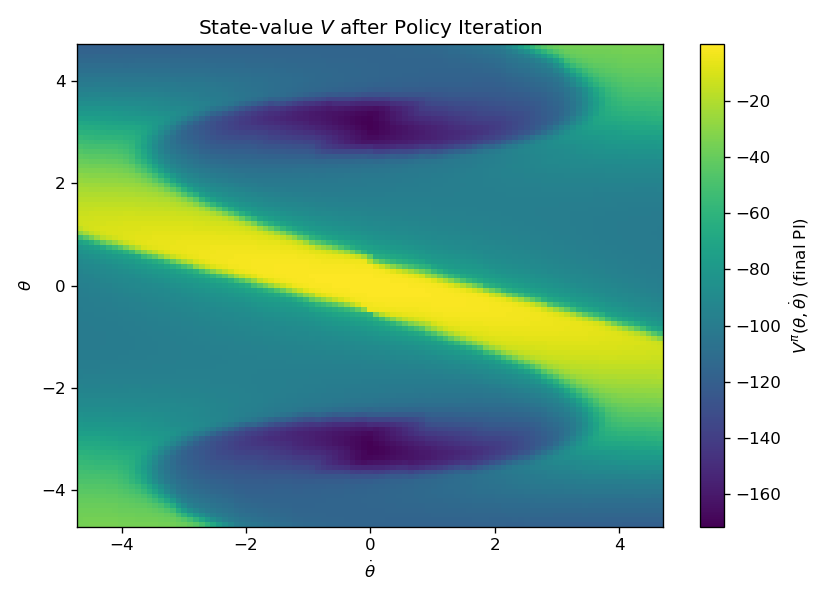
\includegraphics[width=0.8\linewidth]{images/MDP/pendulum_PI_value} 

}

\caption{Optimal Value Function after Policy Iteration}\label{fig:mdp-pendulum-PI-value}
\end{figure}

\begin{figure}

{\centering 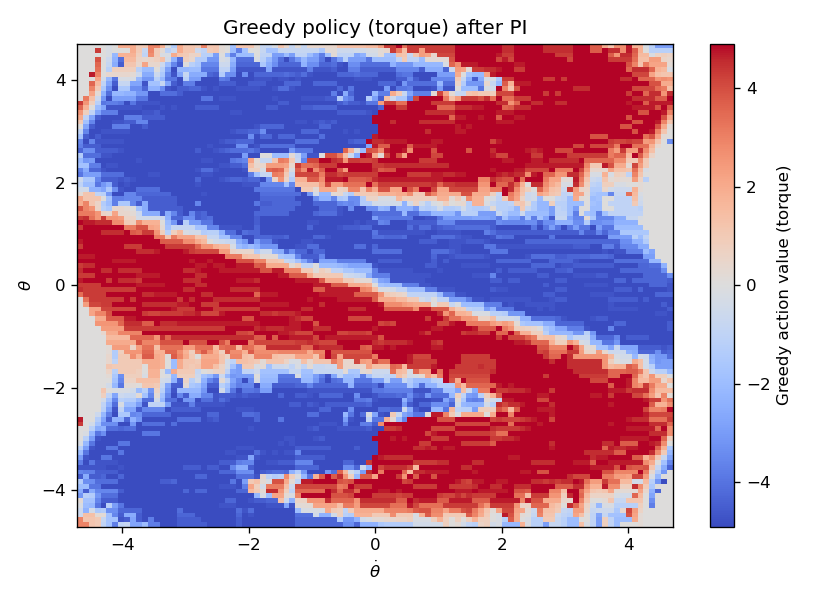
\includegraphics[width=0.8\linewidth]{images/MDP/pendulum_PI_policy} 

}

\caption{Optimal Policy after Policy Iteration}\label{fig:mdp-pendulum-PI-policy}
\end{figure}

We can apply the optimal policy to the pendulum with an initial state of \((-\pi, 0)\) (i.e., the bottomright position). Fig. \ref{fig:mdp-pendulum-PI-rollout-trajectory} plots the rollout trajectory of \(\theta, \dot{\theta}, u\). We can see that the optimal policy is capable of performing ``bang-bang'' control to accumulate energy before swinging up.

Fig. \ref{fig:mdp-pendulum-PI-rollout-trajectory-value} overlays the trajectory on top of the optimal value function.

You can play with the code \href{https://github.com/ComputationalRobotics/2025-ES-AM-158-LECTURE-CODE/blob/main/pendulum_policy_iteration.py}{here}.

\begin{figure}

{\centering 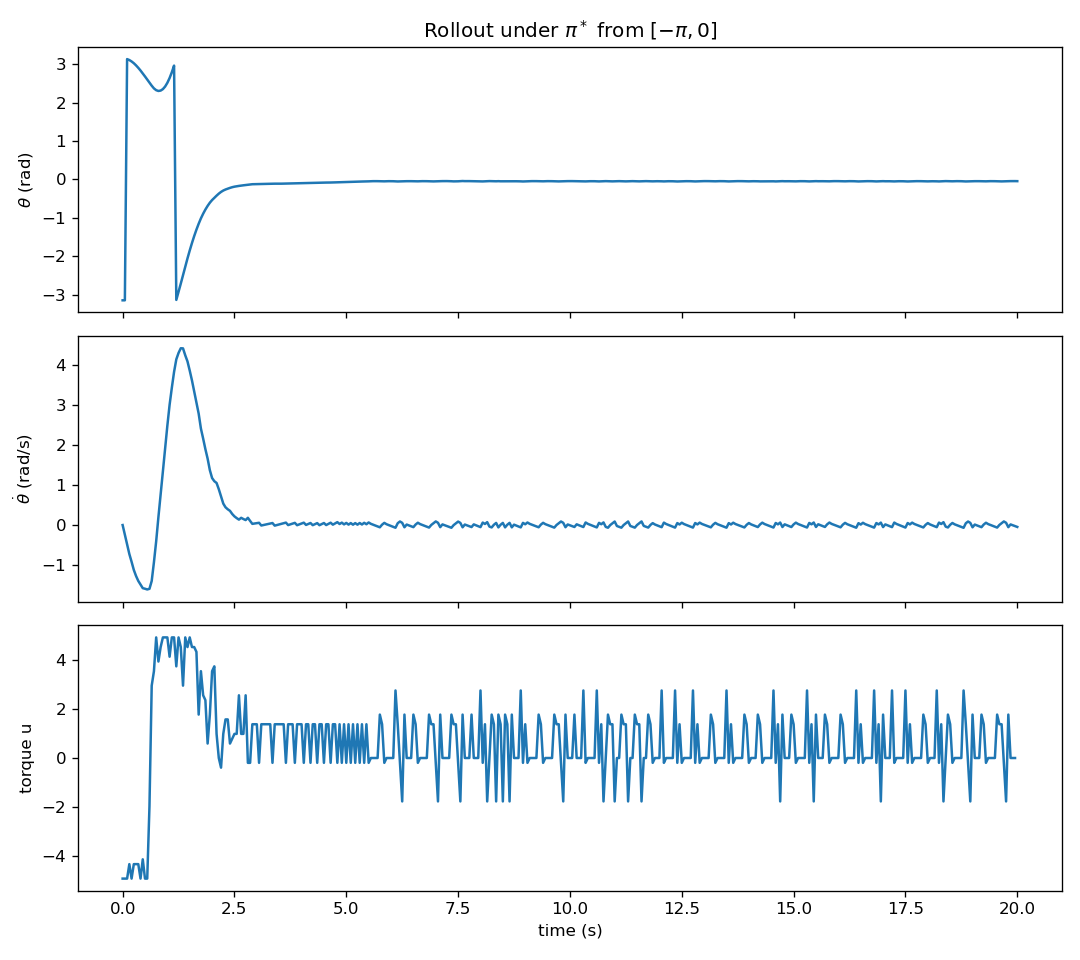
\includegraphics[width=0.9\linewidth]{images/MDP/pendulum_optimal_trajectory} 

}

\caption{Optimal Trajectory of Pendulum Swing-Up}\label{fig:mdp-pendulum-PI-rollout-trajectory}
\end{figure}

\begin{figure}

{\centering 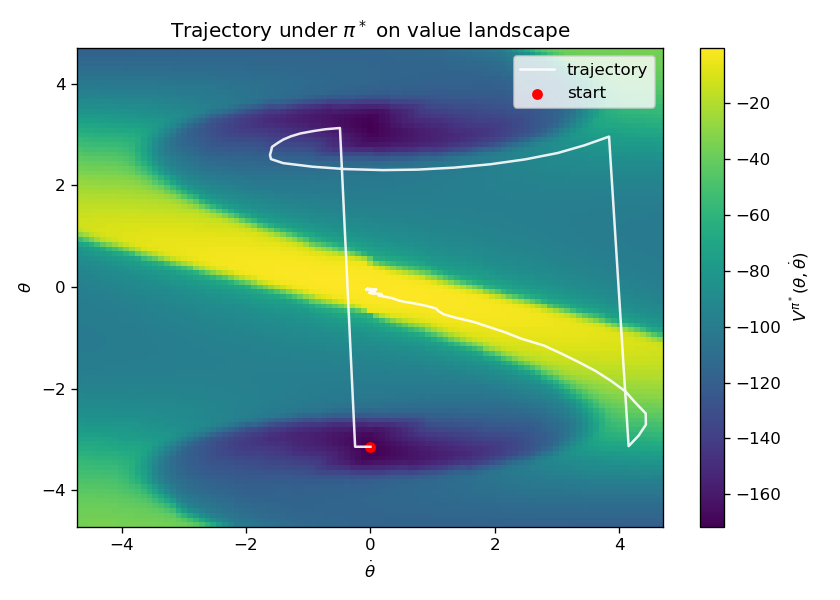
\includegraphics[width=0.9\linewidth]{images/MDP/pendulum_optimal_trajectory_value} 

}

\caption{Optimal Trajectory of Pendulum Swing-Up Overlayed with Optimal Value Function}\label{fig:mdp-pendulum-PI-rollout-trajectory-value}
\end{figure}

\end{example}

\subsection{Value Iteration}\label{value-iteration}

Policy iteration---as the name suggests---iterates on \emph{policies}: it alternates between
(1) \emph{policy evaluation} (computing \(V^{\pi}\) for the current policy \(\pi\)) and
(2) \emph{policy improvement} (making \(\pi\) greedy w.r.t. \(V^{\pi}\)).

An alternative, often very effective, method is \emph{value iteration}. Unlike policy iteration, value iteration does \emph{not} explicitly maintain a policy during its updates; it iterates directly on the value function toward the fixed point of the Bellman optimality* operator. Once the value function has (approximately) converged, the optimal policy is obtained by a single greedy extraction step. Note that intermediate value iterates need not correspond to the value of any actual policy.

The value iteration (VI) algorithm works as follows:

\textbf{Initialization.} Choose any \(V_0:\mathcal{S}\to\mathbb{R}\) (e.g., \(V_0 \equiv 0\)).\\
\textbf{Iteration.} For \(k=0,1,2,\dots\),
\[
V_{k+1}(s) \;\leftarrow\; \max_{a\in\mathcal{A}}
\Big[\, R(s,a) \;+\; \gamma \sum_{s'\in\mathcal{S}} P(s'\mid s,a)\; V_k(s') \,\Big],
\quad \forall s\in\mathcal{S}.
\]
\textbf{Stopping rule.} Stop when \(\lVert V_{k+1}-V_k\rVert_\infty \le \varepsilon\) (or any chosen tolerance).

\textbf{Policy extraction (greedy):}
\[
\pi_{k+1}(s) \in \arg\max_{a\in\mathcal{A}}
\Big[\, R(s,a) \;+\; \gamma \sum_{s'} P(s'\mid s,a)\; V_{k+1}(s') \,\Big].
\]

The following theorem states the convergence of value iteration.

\begin{theorem}[Convergence of Value Iteration]
\protect\hypertarget{thm:ValueIterationConvergence}{}\label{thm:ValueIterationConvergence}Let \(T^\star\) be the Bellman optimality operator,
\[
(T^\star V)(s) := \max_{a}\Big[ R(s,a) + \gamma \sum_{s'} P(s'\mid s,a)\, V(s') \Big].
\]
For \(\gamma\in[0,1)\) and finite \(\mathcal{S},\mathcal{A}\), \(T^\star\) is a \(\gamma\)-contraction in the sup-norm. Hence, for any \(V_0\),
\[
V_k \;=\; (T^\star )^k V_0 \;\xrightarrow[k\to\infty]{}\; V^*,
\]
the unique fixed point of \(T^\star\). Moreover, the greedy policy \(\pi_k\) extracted from \(V_k\) converges to an optimal policy \(\pi^\star\).

In addition, after \(k\) iterations, we have
\[
\lVert V_k - V^* \rVert_\infty \;\le\; \gamma^k \, \lVert V_0 - V^* \rVert_\infty.
\]
\end{theorem}

Finally, we apply value iteration to the inverted pendulum problem.

\begin{example}[Value Iteration for Inverted Pendulum]
\protect\hypertarget{exm:InvertedPendulumValueIteration}{}\label{exm:InvertedPendulumValueIteration}The following code performs value iteration for the inverted pendulum problem.

\begin{Shaded}
\begin{Highlighting}[]
\ImportTok{import}\NormalTok{ numpy }\ImportTok{as}\NormalTok{ np}
\ImportTok{import}\NormalTok{ matplotlib.pyplot }\ImportTok{as}\NormalTok{ plt}

\CommentTok{\# {-}{-}{-}{-}{-} Physical \& MDP parameters {-}{-}{-}{-}{-}}
\NormalTok{g, l, m, c }\OperatorTok{=} \FloatTok{9.81}\NormalTok{, }\FloatTok{1.0}\NormalTok{, }\FloatTok{1.0}\NormalTok{, }\FloatTok{0.1}
\NormalTok{dt }\OperatorTok{=} \FloatTok{0.05}
\NormalTok{gamma }\OperatorTok{=} \FloatTok{0.97}
\NormalTok{eps }\OperatorTok{=} \FloatTok{1e{-}8}

\CommentTok{\# Grids}
\NormalTok{N\_theta }\OperatorTok{=} \DecValTok{101}
\NormalTok{N\_thetadot }\OperatorTok{=} \DecValTok{101}
\NormalTok{N\_u }\OperatorTok{=} \DecValTok{51}

\NormalTok{theta\_grid }\OperatorTok{=}\NormalTok{ np.linspace(}\OperatorTok{{-}}\FloatTok{1.5}\OperatorTok{*}\NormalTok{np.pi, }\FloatTok{1.5}\OperatorTok{*}\NormalTok{np.pi, N\_theta)}
\NormalTok{thetadot\_grid }\OperatorTok{=}\NormalTok{ np.linspace(}\OperatorTok{{-}}\FloatTok{1.5}\OperatorTok{*}\NormalTok{np.pi, }\FloatTok{1.5}\OperatorTok{*}\NormalTok{np.pi, N\_thetadot)}
\NormalTok{u\_max }\OperatorTok{=} \FloatTok{0.5} \OperatorTok{*}\NormalTok{ m }\OperatorTok{*}\NormalTok{ g }\OperatorTok{*}\NormalTok{ l}
\NormalTok{u\_grid }\OperatorTok{=}\NormalTok{ np.linspace(}\OperatorTok{{-}}\NormalTok{u\_max, u\_max, N\_u)}

\CommentTok{\# Helpers to index/unwrap}
\KeywordTok{def}\NormalTok{ wrap\_angle(x):}
    \ControlFlowTok{return}\NormalTok{ np.arctan2(np.sin(x), np.cos(x))}

\KeywordTok{def}\NormalTok{ state\_index(i, j):}
    \ControlFlowTok{return}\NormalTok{ i }\OperatorTok{*}\NormalTok{ N\_thetadot }\OperatorTok{+}\NormalTok{ j}

\KeywordTok{def}\NormalTok{ index\_to\_state(idx):}
\NormalTok{    i }\OperatorTok{=}\NormalTok{ idx }\OperatorTok{//}\NormalTok{ N\_thetadot}
\NormalTok{    j }\OperatorTok{=}\NormalTok{ idx }\OperatorTok{\%}\NormalTok{ N\_thetadot}
    \ControlFlowTok{return}\NormalTok{ theta\_grid[i], thetadot\_grid[j]}

\NormalTok{S }\OperatorTok{=}\NormalTok{ N\_theta }\OperatorTok{*}\NormalTok{ N\_thetadot}
\NormalTok{A }\OperatorTok{=}\NormalTok{ N\_u}

\CommentTok{\# {-}{-}{-}{-}{-} Dynamics step (continuous {-}\textgreater{} one Euler step) {-}{-}{-}{-}{-}}
\KeywordTok{def}\NormalTok{ step\_euler(theta, thetadot, u):}
\NormalTok{    theta\_next }\OperatorTok{=}\NormalTok{ wrap\_angle(theta }\OperatorTok{+}\NormalTok{ dt }\OperatorTok{*}\NormalTok{ thetadot)}
\NormalTok{    thetadot\_next }\OperatorTok{=}\NormalTok{ thetadot }\OperatorTok{+}\NormalTok{ dt }\OperatorTok{*}\NormalTok{ ((g}\OperatorTok{/}\NormalTok{l) }\OperatorTok{*}\NormalTok{ np.sin(theta) }\OperatorTok{+}\NormalTok{ (}\DecValTok{1}\OperatorTok{/}\NormalTok{(m}\OperatorTok{*}\NormalTok{l}\OperatorTok{*}\NormalTok{l))}\OperatorTok{*}\NormalTok{u }\OperatorTok{{-}}\NormalTok{ c}\OperatorTok{*}\NormalTok{thetadot)}
    \CommentTok{\# clip angular velocity to grid range (bounded MDP)}
\NormalTok{    thetadot\_next }\OperatorTok{=}\NormalTok{ np.clip(thetadot\_next, thetadot\_grid[}\DecValTok{0}\NormalTok{], thetadot\_grid[}\OperatorTok{{-}}\DecValTok{1}\NormalTok{])}
    \ControlFlowTok{return}\NormalTok{ theta\_next, thetadot\_next}

\CommentTok{\# {-}{-}{-}{-}{-} Find 3 nearest grid states and probability weights (inverse{-}distance) {-}{-}{-}{-}{-}}
\NormalTok{grid\_pts }\OperatorTok{=}\NormalTok{ np.stack(np.meshgrid(theta\_grid, thetadot\_grid, indexing}\OperatorTok{=}\StringTok{\textquotesingle{}ij\textquotesingle{}}\NormalTok{), axis}\OperatorTok{={-}}\DecValTok{1}\NormalTok{).reshape(}\OperatorTok{{-}}\DecValTok{1}\NormalTok{, }\DecValTok{2}\NormalTok{)}

\KeywordTok{def}\NormalTok{ nearest3\_probs(theta\_next, thetadot\_next):}
\NormalTok{    x }\OperatorTok{=}\NormalTok{ np.array([theta\_next, thetadot\_next])}
\NormalTok{    dists }\OperatorTok{=}\NormalTok{ np.linalg.norm(grid\_pts }\OperatorTok{{-}}\NormalTok{ x[}\VariableTok{None}\NormalTok{, :], axis}\OperatorTok{=}\DecValTok{1}\NormalTok{)}
\NormalTok{    nn\_idx }\OperatorTok{=}\NormalTok{ np.argpartition(dists, }\DecValTok{3}\NormalTok{)[:}\DecValTok{3}\NormalTok{]      }\CommentTok{\# three smallest (unordered)}
\NormalTok{    nn\_idx }\OperatorTok{=}\NormalTok{ nn\_idx[np.argsort(dists[nn\_idx])]  }\CommentTok{\# sort those 3 by distance}
\NormalTok{    d }\OperatorTok{=}\NormalTok{ dists[nn\_idx]}
\NormalTok{    w }\OperatorTok{=} \FloatTok{1.0} \OperatorTok{/}\NormalTok{ (d }\OperatorTok{+}\NormalTok{ eps)}
\NormalTok{    p }\OperatorTok{=}\NormalTok{ w }\OperatorTok{/}\NormalTok{ w.}\BuiltInTok{sum}\NormalTok{()}
    \ControlFlowTok{return}\NormalTok{ nn\_idx.astype(}\BuiltInTok{int}\NormalTok{), p}

\CommentTok{\# {-}{-}{-}{-}{-} Reward {-}{-}{-}{-}{-}}
\KeywordTok{def}\NormalTok{ reward(theta, thetadot, u):}
    \ControlFlowTok{return} \OperatorTok{{-}}\NormalTok{(theta}\OperatorTok{**}\DecValTok{2} \OperatorTok{+} \FloatTok{0.1}\OperatorTok{*}\NormalTok{thetadot}\OperatorTok{**}\DecValTok{2} \OperatorTok{+} \FloatTok{0.01}\OperatorTok{*}\NormalTok{u}\OperatorTok{**}\DecValTok{2}\NormalTok{)}

\CommentTok{\# {-}{-}{-}{-}{-} Build tabular MDP: R[s,a] and sparse P[s,a,3] {-}{-}{-}{-}{-}}
\NormalTok{R }\OperatorTok{=}\NormalTok{ np.zeros((S, A))}
\NormalTok{NS\_idx }\OperatorTok{=}\NormalTok{ np.zeros((S, A, }\DecValTok{3}\NormalTok{), dtype}\OperatorTok{=}\BuiltInTok{int}\NormalTok{)   }\CommentTok{\# next{-}state indices (3 nearest)}
\NormalTok{NS\_prob }\OperatorTok{=}\NormalTok{ np.zeros((S, A, }\DecValTok{3}\NormalTok{))             }\CommentTok{\# their probabilities}

\ControlFlowTok{for}\NormalTok{ i, th }\KeywordTok{in} \BuiltInTok{enumerate}\NormalTok{(theta\_grid):}
    \ControlFlowTok{for}\NormalTok{ j, thd }\KeywordTok{in} \BuiltInTok{enumerate}\NormalTok{(thetadot\_grid):}
\NormalTok{        s }\OperatorTok{=}\NormalTok{ state\_index(i, j)}
        \ControlFlowTok{for}\NormalTok{ a, u }\KeywordTok{in} \BuiltInTok{enumerate}\NormalTok{(u\_grid):}
\NormalTok{            R[s, a] }\OperatorTok{=}\NormalTok{ reward(th, thd, u)}
\NormalTok{            th\_n, thd\_n }\OperatorTok{=}\NormalTok{ step\_euler(th, thd, u)}
\NormalTok{            nn\_idx, p }\OperatorTok{=}\NormalTok{ nearest3\_probs(th\_n, thd\_n)}
\NormalTok{            NS\_idx[s, a, :] }\OperatorTok{=}\NormalTok{ nn\_idx}
\NormalTok{            NS\_prob[s, a, :] }\OperatorTok{=}\NormalTok{ p}

\CommentTok{\# =======================}
\CommentTok{\#       VALUE ITERATION}
\CommentTok{\# =======================}

\CommentTok{\# Bellman optimality update:}
\CommentTok{\# V\_\{k+1\}(s) = max\_a [ R(s,a) + gamma * sum\_j P(s,a,j) * V\_k(ns\_j) ]}
\NormalTok{V }\OperatorTok{=}\NormalTok{ np.zeros(S)}
\NormalTok{tol }\OperatorTok{=} \FloatTok{1e{-}6}
\NormalTok{max\_vi\_iters }\OperatorTok{=} \DecValTok{1000}

\ControlFlowTok{for}\NormalTok{ k }\KeywordTok{in} \BuiltInTok{range}\NormalTok{(max\_vi\_iters):}
    \CommentTok{\# Expected next V for every (s,a), given current V\_k}
\NormalTok{    EV\_next }\OperatorTok{=}\NormalTok{ (NS\_prob }\OperatorTok{*}\NormalTok{ V[NS\_idx]).}\BuiltInTok{sum}\NormalTok{(axis}\OperatorTok{=}\DecValTok{2}\NormalTok{)   }\CommentTok{\# shape (S, A)}
\NormalTok{    Q }\OperatorTok{=}\NormalTok{ R }\OperatorTok{+}\NormalTok{ gamma }\OperatorTok{*}\NormalTok{ EV\_next                       }\CommentTok{\# shape (S, A)}
\NormalTok{    V\_new }\OperatorTok{=}\NormalTok{ np.}\BuiltInTok{max}\NormalTok{(Q, axis}\OperatorTok{=}\DecValTok{1}\NormalTok{)                     }\CommentTok{\# greedy backup over actions}

\NormalTok{    delta }\OperatorTok{=}\NormalTok{ np.}\BuiltInTok{max}\NormalTok{(np.}\BuiltInTok{abs}\NormalTok{(V\_new }\OperatorTok{{-}}\NormalTok{ V))}
    \CommentTok{\# Optional: a stopping rule aligned with policy loss bound could scale tol}
    \CommentTok{\# e.g., stop when delta \textless{}= tol * (1 {-} gamma) / (2 * gamma)}
    \ControlFlowTok{if}\NormalTok{ delta }\OperatorTok{\textless{}}\NormalTok{ tol:}
\NormalTok{        V }\OperatorTok{=}\NormalTok{ V\_new}
        \BuiltInTok{print}\NormalTok{(}\SpecialStringTok{f"Value Iteration converged in }\SpecialCharTok{\{}\NormalTok{k}\OperatorTok{+}\DecValTok{1}\SpecialCharTok{\}}\SpecialStringTok{ iterations (sup{-}norm change }\SpecialCharTok{\{}\NormalTok{delta}\SpecialCharTok{:.2e\}}\SpecialStringTok{)."}\NormalTok{)}
        \ControlFlowTok{break}
\NormalTok{    V }\OperatorTok{=}\NormalTok{ V\_new}
\ControlFlowTok{else}\NormalTok{:}
    \BuiltInTok{print}\NormalTok{(}\SpecialStringTok{f"Reached max\_vi\_iters=}\SpecialCharTok{\{}\NormalTok{max\_vi\_iters}\SpecialCharTok{\}}\SpecialStringTok{ (last sup{-}norm change }\SpecialCharTok{\{}\NormalTok{delta}\SpecialCharTok{:.2e\}}\SpecialStringTok{)."}\NormalTok{)}

\CommentTok{\# Greedy policy extraction from the final V}
\NormalTok{EV\_next }\OperatorTok{=}\NormalTok{ (NS\_prob }\OperatorTok{*}\NormalTok{ V[NS\_idx]).}\BuiltInTok{sum}\NormalTok{(axis}\OperatorTok{=}\DecValTok{2}\NormalTok{)   }\CommentTok{\# recompute with final V}
\NormalTok{Q }\OperatorTok{=}\NormalTok{ R }\OperatorTok{+}\NormalTok{ gamma }\OperatorTok{*}\NormalTok{ EV\_next}
\NormalTok{pi }\OperatorTok{=}\NormalTok{ np.argmax(Q, axis}\OperatorTok{=}\DecValTok{1}\NormalTok{)                     }\CommentTok{\# deterministic greedy policy (indices)}

\CommentTok{\# {-}{-}{-}{-}{-} Visualization: Value function {-}{-}{-}{-}{-}}
\NormalTok{V\_grid }\OperatorTok{=}\NormalTok{ V.reshape(N\_theta, N\_thetadot)}

\NormalTok{fig, ax }\OperatorTok{=}\NormalTok{ plt.subplots(figsize}\OperatorTok{=}\NormalTok{(}\DecValTok{7}\NormalTok{,}\DecValTok{5}\NormalTok{), dpi}\OperatorTok{=}\DecValTok{120}\NormalTok{)}
\NormalTok{im }\OperatorTok{=}\NormalTok{ ax.imshow(}
\NormalTok{    V\_grid,}
\NormalTok{    origin}\OperatorTok{=}\StringTok{"lower"}\NormalTok{,}
\NormalTok{    extent}\OperatorTok{=}\NormalTok{[thetadot\_grid.}\BuiltInTok{min}\NormalTok{(), thetadot\_grid.}\BuiltInTok{max}\NormalTok{(),}
\NormalTok{            theta\_grid.}\BuiltInTok{min}\NormalTok{(), theta\_grid.}\BuiltInTok{max}\NormalTok{()],}
\NormalTok{    aspect}\OperatorTok{=}\StringTok{"auto"}\NormalTok{,}
\NormalTok{    cmap}\OperatorTok{=}\StringTok{"viridis"}
\NormalTok{)}
\NormalTok{cbar }\OperatorTok{=}\NormalTok{ fig.colorbar(im, ax}\OperatorTok{=}\NormalTok{ax)}
\NormalTok{cbar.set\_label(}\VerbatimStringTok{r"$V\^{}*(\textbackslash{}theta,\textbackslash{}dot\{\textbackslash{}theta\})$ (Value Iteration)"}\NormalTok{)}

\NormalTok{ax.set\_xlabel(}\VerbatimStringTok{r"$\textbackslash{}dot\{\textbackslash{}theta\}$"}\NormalTok{)}
\NormalTok{ax.set\_ylabel(}\VerbatimStringTok{r"$\textbackslash{}theta$"}\NormalTok{)}
\NormalTok{ax.set\_title(}\VerbatimStringTok{r"State{-}value $V$ after Value Iteration"}\NormalTok{)}

\NormalTok{plt.tight\_layout()}
\NormalTok{plt.show()}

\CommentTok{\# {-}{-}{-}{-}{-} Visualization: Greedy torque field {-}{-}{-}{-}{-}}
\NormalTok{pi\_grid }\OperatorTok{=}\NormalTok{ pi.reshape(N\_theta, N\_thetadot)   }\CommentTok{\# action indices}
\NormalTok{action\_values }\OperatorTok{=}\NormalTok{ u\_grid[pi\_grid]             }\CommentTok{\# map indices {-}\textgreater{} torques}

\NormalTok{plt.figure(figsize}\OperatorTok{=}\NormalTok{(}\DecValTok{7}\NormalTok{,}\DecValTok{5}\NormalTok{), dpi}\OperatorTok{=}\DecValTok{120}\NormalTok{)}
\NormalTok{im }\OperatorTok{=}\NormalTok{ plt.imshow(}
\NormalTok{    action\_values,}
\NormalTok{    origin}\OperatorTok{=}\StringTok{"lower"}\NormalTok{,}
\NormalTok{    extent}\OperatorTok{=}\NormalTok{[thetadot\_grid.}\BuiltInTok{min}\NormalTok{(), thetadot\_grid.}\BuiltInTok{max}\NormalTok{(),}
\NormalTok{            theta\_grid.}\BuiltInTok{min}\NormalTok{(), theta\_grid.}\BuiltInTok{max}\NormalTok{()],}
\NormalTok{    aspect}\OperatorTok{=}\StringTok{"auto"}\NormalTok{,}
\NormalTok{    cmap}\OperatorTok{=}\StringTok{"coolwarm"}   \CommentTok{\# good for ± torque}
\NormalTok{)}
\NormalTok{cbar }\OperatorTok{=}\NormalTok{ plt.colorbar(im)}
\NormalTok{cbar.set\_label(}\StringTok{"Greedy action value (torque)"}\NormalTok{)}

\NormalTok{plt.xlabel(}\VerbatimStringTok{r"$\textbackslash{}dot\{\textbackslash{}theta\}$"}\NormalTok{)}
\NormalTok{plt.ylabel(}\VerbatimStringTok{r"$\textbackslash{}theta$"}\NormalTok{)}
\NormalTok{plt.title(}\StringTok{"Greedy policy (torque) extracted from Value Iteration"}\NormalTok{)}
\NormalTok{plt.tight\_layout()}
\NormalTok{plt.show()}
\end{Highlighting}
\end{Shaded}

Try it for yourself \href{https://github.com/ComputationalRobotics/2025-ES-AM-158-LECTURE-CODE/blob/main/pendulum_value_iteration.py}{here}!

You should obtain the same results as policy iteration.
\end{example}

\chapter{Value-based Reinforcement Learning}\label{value-rl}

In Chapter \ref{mdp}, we introduced algorithms for policy evaluation, policy improvement, and computing optimal policies in the tabular setting when the model is known. These dynamic-programming methods are grounded in Bellman consistency and optimality and come with strong convergence guarantees.

A key limitation of the methods in Chapter \ref{mdp} is that they require the transition dynamics \(P(s' \mid s, a)\) to be known. While in some applications modeling the dynamics is feasible (e.g., the inverted pendulum), in many others it is costly or impractical to obtain an accurate model of the environment (e.g., a humanoid robot interacting with everyday objects).

This motivates relaxing the known-dynamics assumption and asking whether we can design algorithms that learn purely from interaction---i.e., by collecting data through environment interaction. This brings us to \textbf{model-free reinforcement learning}.

In this chapter we focus on \textbf{value-based} RL methods. The central idea is to learn the value functions---\(V(s)\) and \(Q(s,a)\)---from interaction with the environment and then leverage these estimates to derive (approximately) optimal policies. We begin with tabular methods and then move to function-approximation approaches (e.g., neural networks) for problems where a tabular representation is intractable.

\section{Tabular Methods}\label{tabular-methods}

Consider an infinite-horizon Markov decision process (MDP)\\
\[
\mathcal{M} = (\mathcal{S}, \mathcal{A}, P, R, \gamma),
\]
with a discount factor \(\gamma \in [0,1)\). We focus on the \emph{tabular setting} where both the state space \(\mathcal{S}\) and the action space \(\mathcal{A}\) are finite, with cardinalities \(|\mathcal{S}|\) and \(|\mathcal{A}|\), respectively.

A policy is a stationary stochastic mapping\\
\[
\pi: \mathcal{S} \to \Delta(\mathcal{A}),
\]
where \(\pi(a \mid s)\) denotes the probability of selecting action \(a\) in state \(s\).

Unlike in Chapter \ref{mdp}, here we do not assume knowledge of the transition dynamics \(P\) or the reward function \(R\) (other than that \(R\) is deterministic). Instead, we assume we can interact with the environment and obtain \emph{trajectories} of the form\\
\[
\tau = (s_0, a_0, r_0, s_1, a_1, r_1, \dots),
\]
by following a policy \(\pi\).

\subsection{Policy Evaluation}\label{policy-evaluation-2}

We first consider the problem of estimating the value function of a given policy \(\pi\). Recall the definition of the state-value function associated with \(\pi\) is:
\begin{equation}
V^{\pi}(s) = \mathbb{E}\left[ \sum_{t=0}^{\infty} \gamma^t R(s_t, a_t) \mid s_0 = s \right],
\label{eq:InfiniteHorizonStateValueRestate}
\end{equation}
where the expectation is taken over the randomness of both the policy \(\pi\) and the transition dynamics \(P\).

\subsubsection{Monte Carlo Estimation}\label{monte-carlo-estimation}

The basic idea of Monte Carlo (MC) estimation is to approximate the value function \(V^\pi\) by averaging \emph{empirical returns} observed from sampled trajectories generated under policy \(\pi\). Since the return is defined as the discounted sum of future rewards, MC methods replace the expectation in the definition of \(V^\pi\) with an average over sampled trajectories.

\textbf{Episodic Assumption.} To make Monte Carlo methods well-defined, we restrict attention to the \emph{episodic setup}, where each trajectory terminates upon reaching a terminal state (and the rewards thereafter are always zero). This ensures that the return is finite and can be computed exactly for each trajectory. Concretely, if an episode terminates at time \(T\), the return starting from time \(t\) is
\begin{equation}
g_t = \sum_{k=0}^{T-t-1} \gamma^k r_{t+k} = r_t + \gamma r_{t+1} + \gamma^2 r_{t+2} + \dots + \gamma^{T-t-1} r_{T-1}.
\label{eq:return-MC}
\end{equation}

\textbf{Algorithmic Form.} Let \(\mathcal{D}(s)\) denote the set of all time indices at which state \(s\) is visited across sampled episodes. Then the Monte Carlo estimate of the value function is
\begin{equation}
\hat{V}(s) = \frac{1}{|\mathcal{D}(s)|} \sum_{t \in \mathcal{D}(s)} g_t.
\label{eq:StateValueMCEstimate}
\end{equation}

There are two common variants:

\begin{itemize}
\tightlist
\item
  \textbf{First-visit MC:} use only the first occurrence of \(s\) in each episode.\\
\item
  \textbf{Every-visit MC:} use all occurrences of \(s\) within an episode.
\end{itemize}

Both variants converge to the same value function in the limit of infinitely many episodes.

\textbf{Incremental Implementation.} Monte Carlo can be written as an incremental stochastic-approximation update that uses the return \(g_t\) as the \emph{target} and a \emph{diminishing step size}. Let \(N(s)\) be the number of (first- or every-) visits to state \(s\) that have been used to update \(\hat V(s)\) so far, and let \(g_t\) be the return computed at a particular visit time \(t\in\mathcal{D}(s)\). Then the MC update is
\begin{equation}
\hat V(s) \;\leftarrow\; \hat V(s) + \alpha_{N(s)}\,\big( g_t - \hat V(s) \big),
\qquad \alpha_{N(s)} > 0 \text{ diminishing.}
\label{eq:mc-incremental}
\end{equation}
A canonical choice is the \emph{sample-average} step size \(\alpha_{N(s)} = 1/N(s)\), which yields the recurrence
\begin{align}
\hat V_{N}(s) = \hat V_{N-1}(s) + \tfrac{1}{N}\big(g_t - \hat V_{N-1}(s)\big)
& = \Big(1-\tfrac{1}{N}\Big)\hat V_{N-1}(s) + \tfrac{1}{N}\, g_t \\
& = \frac{N-1}{N} \frac{1}{N-1} \sum_{i=1}^{N-1} g_{t,i} + \frac{1}{N} g_t \\
& = \frac{1}{N} \sum_{i=1}^N g_{t,i}
\end{align}
so that \(\hat V_{N}(s)\) equals the average of the \(N\) observed returns for \(s\) (i.e., Eq. \eqref{eq:StateValueMCEstimate}). In the above equation, I have used \(g_{t,i}\) to denote the \(i\)-th return before \(g_t\) was collected (and \(g_t = g_{t,N}\)). More generally, any diminishing schedule satisfying
\[
\sum_{n=1}^\infty \alpha_n = \infty, \qquad \sum_{n=1}^\infty \alpha_n^2 < \infty
\]
(e.g., \(\alpha_n = c/(n+t_0)^p\) with \(1/2 < p \le 1\)) also ensures consistency in the tabular setting. In first-visit MC, \(N(s)\) increases by one per episode at most; in every-visit MC, \(N(s)\) increases at each occurrence of \(s\) within an episode.

\textbf{Theoretical Guarantees.}

\begin{enumerate}
\def\labelenumi{\arabic{enumi}.}
\tightlist
\item
  \textbf{Unbiasedness:} For any state \(s\), the return \(g_t\) is an unbiased sample of \(V^\pi(s)\).\\
  \[
  \mathbb{E}[g_t \mid s_t = s] = V^\pi(s).
  \]
\item
  \textbf{Consistency:} By the law of large numbers, as the number of episodes grows,
  \[
  \hat{V}(s) \xrightarrow{\text{a.s.}} V^\pi(s).
  \]
\item
  \textbf{Asymptotic Normality:} The MC estimator converges at rate \(O(1/\sqrt{N})\), where \(N\) is the number of episodes used for the estimation.
\end{enumerate}

\textbf{Limitations.} Despite its conceptual simplicity, MC estimation suffers from several drawbacks:

\begin{itemize}
\item
  It requires \emph{episodes to terminate}, making it unsuitable for continuing tasks without artificial truncation.
\item
  It can only update value estimates \emph{after an episode ends}, which is data-inefficient.
\item
  While unbiased, MC estimates often have \emph{high variance}, leading to slow convergence.
\end{itemize}

These limitations motivate the study of \emph{Temporal-Difference (TD) learning}, which updates value estimates online and can handle continuing tasks.

\subsubsection{Temporal-Difference Learning}\label{temporal-difference-learning}

While Monte Carlo methods estimate value functions by averaging full returns from complete episodes, Temporal-Difference (TD) learning provides an alternative approach that updates value estimates \emph{incrementally} after each step of interaction with the environment. The key idea is to combine the sampling of Monte Carlo with the \emph{bootstrapping} of dynamic programming.

\textbf{High-Level Intuition.} TD learning avoids waiting until the end of an episode by using the Bellman consistency equation as a basis for updates. Recall that for any policy \(\pi\), the Bellman consistency equation reads:
\begin{equation}
V^\pi(s) = \mathbb{E}_{a \sim \pi(\cdot \mid s)} \left[ R(s,a) + \gamma \mathbb{E}_{s' \sim P(s' \mid s, a)} V(s')  \right].
\label{eq:InfiniteHorizonBellmanConsistencyRestate}
\end{equation}
At a high level, TD learning turns the expectation in Bellman equation into sampling.
At each step, it updates the current estimate of the value function toward a \emph{one-step bootstrap target}: the immediate reward plus the discounted value of the next state. This makes TD methods more data-efficient and applicable to continuing tasks without terminal states.

\textbf{Algorithmic Form.} Suppose the agent is in state \(s_t\), takes action \(a_t \sim \pi(\cdot \mid s_t)\), receives reward \(r_t\), and transitions to \(s_{t+1}\). The TD(0) update rule is
\begin{equation}
\hat{V}(s_t) \;\leftarrow\; \hat{V}(s_t) + \alpha \big[ r_t + \gamma \hat{V}(s_{t+1}) - \hat{V}(s_t) \big],
\label{eq:TDZeroUpdate}
\end{equation}
where \(\alpha \in (0,1]\) is the learning rate.

The term inside the brackets,
\begin{equation}
\delta_t = r_t + \gamma \hat{V}(s_{t+1}) - \hat{V}(s_t),
\label{eq:TDError}
\end{equation}
is called the TD error. It measures the discrepancy between the current value estimate and the bootstrap target. The algorithm updates \(\hat{V}(s_t)\) in the direction of reducing this error.

\textbf{Theoretical Guarantees.}

\begin{enumerate}
\def\labelenumi{\arabic{enumi}.}
\item
  \textbf{Convergence in the Tabular Case:} If each state is visited infinitely often and the learning rate sequence satisfies
  \[
  \sum_t \alpha_t = \infty, \; \sum_t \alpha_t^2 < \infty
  \]
  then TD(0) converges almost surely to the true value function \(V^\pi\). For example, choosing \(\alpha_t = 1/(t+1)\) satisfies this condition. Section \ref{value-rl-convergence-td} provides a detailed proof of the convergence of TD learning.
\item
  \textbf{Bias--Variance Tradeoff:}

  \begin{itemize}
  \item
    The TD target uses the current estimate \(\hat{V}(s_{t+1})\) rather than the true value, which introduces \emph{bias}.
  \item
    However, it has significantly \emph{lower variance} than Monte Carlo estimates, often leading to faster convergence in practice.
  \end{itemize}

  To see this, note that for TD(0), the target is a one-step bootstrap:
  \[
  y_t = r_t + \gamma \hat{V}(s_{t+1}).
  \]
  This replaces the true value \(V^\pi(s_{t+1})\) with the \emph{current estimate} \(\hat{V}(s_{t+1})\). As a result, \(y_t\) is \emph{biased} relative to the true return. However, since it depends only on the immediate reward and the next state, the variance of \(y_t\) is \emph{much lower} than that of the Monte Carlo target.
\end{enumerate}

\textbf{Limitations.}

\begin{itemize}
\item
  TD(0) relies on bootstrapping, which introduces bias relative to Monte Carlo methods.
\item
  Convergence can be slow if the learning rate is not chosen carefully.
\end{itemize}

In summary, Temporal-Difference learning addresses the major limitations of Monte Carlo estimation: it works in \emph{continuing tasks}, updates \emph{online} at each step, and is generally more \emph{sample-efficient}. However, it trades away unbiasedness for bias--variance efficiency, motivating further extensions such as multi-step TD and TD(\(\lambda\)).

\subsubsection{Multi-Step TD Learning}\label{multi-step-td-learning}

Monte Carlo methods use the \emph{full return} \(g_t\), while TD(0) uses a \emph{one-step bootstrap}. Multi-step TD learning generalizes these two extremes by using \(n\)-step returns as targets. In this way, multi-step TD interpolates between Monte Carlo and TD(0).

\textbf{High-Level Intuition.} The motivation is to balance the high variance of Monte Carlo with the bias of TD(0). Instead of waiting for a full return (MC) or using only one step of bootstrapping (TD(0)), multi-step TD uses partial returns spanning \(n\) steps of real rewards, followed by a bootstrap. This provides a flexible tradeoff between bias and variance.

\textbf{Algorithmic Form.} The \(n\)-step return starting from time \(t\) is defined as
\begin{equation}
g_t^{(n)} = r_t + \gamma r_{t+1} + \dots + \gamma^{n-1} r_{t+n-1} + \gamma^n \hat{V}(s_{t+n}).
\label{eq:nStepReturn}
\end{equation}

The \(n\)-step TD update is
\begin{equation}
\hat{V}(s_t) \;\leftarrow\; \hat{V}(s_t) + \alpha \big[ g_t^{(n)} - \hat{V}(s_t) \big],
\label{eq:nStepTDUpdate}
\end{equation}
where \(g_t^{(n)}\) replaces the one-step target in TD(0) \eqref{eq:TDZeroUpdate}.

\begin{itemize}
\item
  For \(n=1\): the method reduces to TD(0).
\item
  For \(n=T-t\) (the full episode length): the method reduces to Monte Carlo.
\end{itemize}

\textbf{Theoretical Guarantees.}

\begin{enumerate}
\def\labelenumi{\arabic{enumi}.}
\item
  \textbf{Convergence in the Tabular Case:} With suitable learning rates and sufficient exploration, \(n\)-step TD converges to \(V^\pi\).
\item
  \textbf{Bias--Variance Tradeoff:}

  \begin{itemize}
  \item
    Larger \(n\): lower bias, higher variance (closer to Monte Carlo).
  \item
    Smaller \(n\): higher bias, lower variance (closer to TD(0)).
  \item
    Intermediate \(n\) provides a balance that often yields faster learning in practice.
  \end{itemize}
\end{enumerate}

\textbf{Limitations.}

\begin{itemize}
\item
  Choosing the right \(n\) is problem-dependent: too small and bias dominates; too large and variance grows.
\item
  Requires storing \(n\)-step reward sequences before updating, which can increase memory and computation.
\end{itemize}

In summary, multi-step TD unifies Monte Carlo and TD(0) by introducing \(n\)-step returns. It allows practitioners to \emph{tune the bias--variance tradeoff} by selecting \(n\). Later, we will see how TD(\(\lambda\)) averages over all \(n\)-step returns in a principled way, further smoothing this tradeoff.

\subsubsection{\texorpdfstring{Eligibility Traces and TD(\(\lambda\))}{Eligibility Traces and TD(\textbackslash lambda)}}\label{eligibility-traces-and-tdlambda}

So far, we have seen that Monte Carlo methods use \emph{full returns} \(g_t\), while TD(0) uses a \emph{one-step bootstrap}. Multi-step TD methods generalize between these two extremes by using \(n\)-step returns. However, a natural question arises: \emph{can we combine information from all possible \(n\)-step returns in a principled way?}

This motivates TD(\(\lambda\)), which blends multi-step TD methods into a single algorithm using \emph{eligibility traces}.

\textbf{High-Level Intuition.} TD(\(\lambda\)) introduces a parameter \(\lambda \in [0,1]\) that controls the weighting of \(n\)-step returns:

\begin{itemize}
\item
  \(\lambda = 0\): reduces to TD(0), relying only on one-step bootstrapping.
\item
  \(\lambda = 1\): reduces to Monte Carlo, relying on full returns.
\item
  \(0 < \lambda < 1\): interpolates smoothly between these two extremes by averaging all \(n\)-step returns with exponentially decaying weights.
\end{itemize}

Formally, the \(\lambda\)-return is
\begin{equation}
g_t^{(\lambda)} = (1-\lambda) \sum_{n=1}^{\infty} \lambda^{n-1} g_t^{(n)},
\label{eq:LambdaReturn}
\end{equation}
where \(g_t^{(n)}\) is the \(n\)-step return defined in \eqref{eq:nStepReturn}.

\begin{remark}
To make the \(\lambda\)-return well defined, we consider two cases.

\textbf{Episodic Case: Well-posed.} If an episode terminates at time \(T\), let \(N=T-t\) be the remaining steps. Then
\begin{equation}
\begin{split}
g_t^{(\lambda)}
& =
(1-\lambda)\sum_{n=1}^{N-1}\lambda^{\,n-1} \, g_t^{(n)}
\;+\;
\lambda^{\,N-1}\, g_t^{(N)}, \\
& = (1-\lambda)\sum_{n=1}^{N}\lambda^{\,n-1} \, g_t^{(n)}
\;+\;
\lambda^{N}\, g_t^{(N)},
\end{split}
\label{eq:lambda-return-episodic}
\end{equation}
where \(g_t^{(n)}\) is the \(n\)-step return (Eq. \eqref{eq:nStepReturn}) and \(g_t^{(N)}\) is the \emph{full} Monte Carlo return (Eq. \eqref{eq:return-MC}).

This expression is well-defined for all \(\lambda\in[0,1]\). Note that the weights form a convex combination:
\[
(1-\lambda)\sum_{n=1}^{N-1}\lambda^{n-1} + \lambda^{N-1}
= 1-\lambda^{N-1}+\lambda^{N-1} = 1.
\]

\textbf{Continuing Case: Limit.} Taking \(\lambda\uparrow 1\) in \eqref{eq:lambda-return-episodic} gives
\[
\lim_{\lambda\uparrow 1} g_t^{(\lambda)}
= g_t^{(N)} = g_t,
\]
so the \(\lambda\)-return \emph{reduces to the Monte Carlo return} at \(\lambda=1\). For continuing tasks (no terminal \(T\)), \(\lambda=1\) is conventionally defined by this same limiting argument, yielding the infinite-horizon discounted return when \(\gamma<1\).
\end{remark}

\textbf{Eligibility Traces.} Naively computing \(g_t^{(\lambda)}\) would require storing and combining infinitely many \(n\)-step returns, which is impractical. Instead, TD(\(\lambda\)) uses eligibility traces to implement this efficiently online.

An eligibility trace is a temporary record that tracks how much each state is ``eligible'' for updates based on how recently and frequently it has been visited. Specifically, for each state \(s\), we maintain a trace \(z_t(s)\) that evolves as
\begin{equation}
z_t(s) = \gamma \lambda z_{t-1}(s) + \mathbf{1}\{s_t = s\},
\label{eq:EligibilityTrace}
\end{equation}
where \(\mathbf{1}\{s_t = s\}\) is an indicator that equals 1 if state \(s\) is visited at time \(t\), and 0 otherwise.

\textbf{TD(\(\lambda\)) Update Rule.} At each time step \(t\), we compute the TD error
\[
\delta_t = r_t + \gamma \hat{V}(s_{t+1}) - \hat{V}(s_t),
\]
as in \eqref{eq:TDError}. Then, for each state \(s\), we update
\begin{equation}
\hat{V}(s) \;\leftarrow\; \hat{V}(s) + \alpha \, \delta_t \, z_t(s).
\label{eq:TDLambdaUpdate}
\end{equation}

Thus, all states with nonzero eligibility traces are updated simultaneously, with the magnitude of the update determined by both the TD error and the eligibility trace. See Proposition \ref{prp:ForwardBackwardEquivalence} below for a justification.

\textbf{Theoretical Guarantees.}

\begin{enumerate}
\def\labelenumi{\arabic{enumi}.}
\item
  In the tabular case, TD(\(\lambda\)) converges almost surely to the true value function \(V^\pi\) under the usual stochastic approximation conditions (sufficient exploration, decaying step sizes).
\item
  The parameter \(\lambda\) directly controls the bias--variance tradeoff:

  \begin{itemize}
  \item
    Smaller \(\lambda\): more bootstrapping, more bias but lower variance.
  \item
    Larger \(\lambda\): less bootstrapping, less bias but higher variance.
  \end{itemize}
\item
  TD(\(\lambda\)) can be shown to converge to the fixed point of the \(\lambda\)-operator, which is itself a contraction mapping.
\end{enumerate}

In summary, eligibility traces provide an elegant mechanism to combine the advantages of Monte Carlo and TD learning. TD(\(\lambda\)) introduces a spectrum of algorithms: at one end TD(0), at the other Monte Carlo, and in between a family of methods balancing bias and variance. In practice, intermediate values such as \(\lambda \approx 0.9\) often work well.

\begin{proposition}[Forward–Backward Equivalence]
\protect\hypertarget{prp:ForwardBackwardEquivalence}{}\label{prp:ForwardBackwardEquivalence}Consider one episode \(s_0,a_0,r_0,\ldots,s_T\) with \(\hat V(s_T)=0\). Let the \textbf{forward view} apply updates at the end of the episode:
\[
\hat V(s_t) \leftarrow \hat V(s_t) + \alpha \big[g_t^{(\lambda)}-\hat V(s_t)\big],
\quad t=0,\ldots,T-1,
\]
where \(g_t^{(\lambda)}\) is the \(\lambda\)-return in \eqref{eq:LambdaReturn} with the \(n\)-step returns \(g_t^{(n)}\) from \eqref{eq:nStepReturn}, and where \(\hat V\) is kept fixed while computing all \(g_t^{(\lambda)}\).

Let the \textbf{backward view} run through the episode once, using the TD error \(\delta_t\) from \eqref{eq:TDError} and eligibility traces \(z_t(s)\) from \eqref{eq:EligibilityTrace}, and then apply the cumulative update
\[
\Delta_{\text{back}} \hat V(s) \;=\; \alpha \sum_{t=0}^{T-1} \delta_t\, z_t(s).
\]

Then, for every state \(s\),
\[
\Delta_{\text{back}} \hat V(s)
\;=\;
\alpha \sum_{t:\, s_t=s}\big[g_t^{(\lambda)}-\hat V(s_t)\big],
\]
i.e., the net parameter change produced by \eqref{eq:TDLambdaUpdate} equals that of the \(\lambda\)-return updates.
\end{proposition}

\begin{proof}
Fix a state \(s\). Using \eqref{eq:EligibilityTrace},
\[
z_t(s)=\sum_{k=0}^{t}(\gamma\lambda)^{\,t-k}\,\mathbf{1}\{s_k=s\}.
\]
Hence
\[
\sum_{t=0}^{T-1}\delta_t z_t(s)
=\sum_{t=0}^{T-1}\delta_t \sum_{k=0}^{t}(\gamma\lambda)^{\,t-k}\mathbf{1}\{s_k=s\}
=\sum_{k:\,s_k=s}\; \sum_{t=k}^{T-1} (\gamma\lambda)^{\,t-k}\delta_t .
\tag{1}
\]

Write \(\delta_t=r_t+\gamma\hat V(s_{t+1})-\hat V(s_t)\) and split the inner sum:
\[
\sum_{t=k}^{T-1} (\gamma\lambda)^{t-k}\delta_t
= \underbrace{\sum_{t=k}^{T-1} \gamma^{t-k}\lambda^{t-k} r_t}_{\text{(A)}}
+ \underbrace{\sum_{t=k}^{T-1}\gamma^{t-k}\lambda^{t-k}(\gamma\hat V(s_{t+1})-\hat V(s_t))}_{\text{(B)}}.
\]

Term (B) telescopes. Shifting index in the first part of (B),
\[
\sum_{t=k}^{T-1}\gamma^{t-k}\lambda^{t-k}\gamma \hat V(s_{t+1})
= \sum_{t=k+1}^{T}\gamma^{t-k}\lambda^{t-1-k}\hat V(s_t).
\]
Therefore
\[
\text{(B)}=
-\hat V(s_k) 
+ \sum_{t=k+1}^{T-1}\gamma^{t-k}\lambda^{t-1-k}(1-\lambda)\hat V(s_t)
+ \underbrace{\gamma^{T-k}\lambda^{T-1-k}\hat V(s_T)}_{=\,0}.
\tag{2}
\]

Combining (A) and (2), and reindexing with \(n=t-k\),
\[
\sum_{t=k}^{T-1} (\gamma\lambda)^{t-k}\delta_t
= -\hat V(s_k)
+ \sum_{n=0}^{T-1-k}\gamma^{n}\lambda^{n} r_{k+n}
+ (1-\lambda)\sum_{n=1}^{T-1-k}\gamma^{n}\lambda^{n-1}\hat V(s_{k+n}).
\tag{3}
\]

On the other hand, expanding the \(\lambda\)-return \eqref{eq:LambdaReturn},
\[
\begin{aligned}
g_k^{(\lambda)}
&=(1-\lambda)\sum_{n=1}^{T-k}\lambda^{n-1}
\Bigg(\sum_{m=0}^{n-1}\gamma^{m} r_{k+m} + \gamma^{n}\hat V(s_{k+n})\Bigg) + \lambda^{T-k} g_k^{(T-k)}\\
&= \sum_{n=0}^{T-1-k}\gamma^{n}\lambda^{n} r_{k+n}
+ (1-\lambda)\sum_{n=1}^{T-1-k}\gamma^{n}\lambda^{n-1}\hat V(s_{k+n}),
\end{aligned}
\tag{4}
\]
where we used that \(\hat V(s_T)=0\). Comparing (3) and (4) yields
\[
\sum_{t=k}^{T-1} (\gamma\lambda)^{t-k}\delta_t
= g_k^{(\lambda)} - \hat V(s_k).
\tag{5}
\]

Substituting (5) into (1) and multiplying by \(\alpha\) completes the proof.
\end{proof}

\begin{example}[Policy Evaluation (MC and TD Family)]
\protect\hypertarget{exm:PolicyEvaluationRandomWalk}{}\label{exm:PolicyEvaluationRandomWalk}We consider the classic random-walk MDP with terminal states:

\begin{itemize}
\tightlist
\item
  \textbf{States:} \(\{0,1,2,3,4,5,6\}\), where \(0\) and \(6\) are terminal; nonterminal states are \(1{:}5\).
\item
  \textbf{Actions:} \(\{-1,+1\}\) (``Left''/``Right'').
\item
  \textbf{Dynamics:} From a nonterminal state \(s\in\{1,\dots,5\}\), action \(-1\) moves to \(s-1\), and action \(+1\) moves to \(s+1\).
\item
  \textbf{Rewards:} Transitioning into state \(6\) yields reward \(+1\); all other transitions yield \(0\).
\item
  \textbf{Discount:} \(\gamma=1\) (episodic task). Episodes start at state \(s_0=3\) and terminate upon reaching \(\{0,6\}\).
\end{itemize}

We evaluate the \emph{equiprobable policy} \(\pi\) that chooses Left/Right with probability \(1/2\) each at every nonterminal state. Under this policy, the true state-value function on nonterminal states \(s\in\{1,\dots,5\}\) is
\begin{equation}
V^\pi(s) \;=\; \frac{s}{6}.
\label{eq:trueV-rw}
\end{equation}

We compare four \emph{tabular policy-evaluation} methods:

\begin{enumerate}
\def\labelenumi{\arabic{enumi}.}
\item
  \textbf{Monte Carlo (MC), first-visit} --- using full returns as target.
\item
  \textbf{TD(0)} --- one-step bootstrap.
\item
  \textbf{\(n\)-step TD} --- here we use \(n=3\) (intermediate between MC and TD(0)).
\item
  \textbf{TD(\(\lambda\))} --- accumulating eligibility traces (we illustrate with \(\lambda=0.9\)).
\end{enumerate}

All methods estimate \(V^\pi\) from trajectories generated by \(\pi\).

\textbf{Error Metric.}
We report the \emph{mean-squared error (MSE)} over nonterminal states after each episode:
\begin{equation}
\mathrm{MSE}_t \;=\; \frac{1}{5}\sum_{s=1}^{5}\big(\hat V_t(s)-V^\pi(s)\big)^2,
\label{eq:mse-metric}
\end{equation}
where \(V^\pi\) is given by \eqref{eq:trueV-rw}. Curves are averaged over multiple random seeds.

\textbf{Fixed Step Sizes.}
We first use a fixed step size \(\alpha=0.1\) for all methods. Fig. \ref{fig:policy-evaluation-random-walk-fixed-step-size} shows the trajectories of MSE versus number of episodes. We can see that, when using a constant step size, these methods do not converge to exactly the true value function, but to a small neighborhood. In addition, if the algorithm initially decays very fast, then the final variance is larger. For example, MC initially decays very fast, but has a higher variance, whereas TD(0) initially decays slower, but has a lower final variance. This agrees with the theoretical analysis in \citep{kearns2000bias}.

\begin{figure}

{\centering 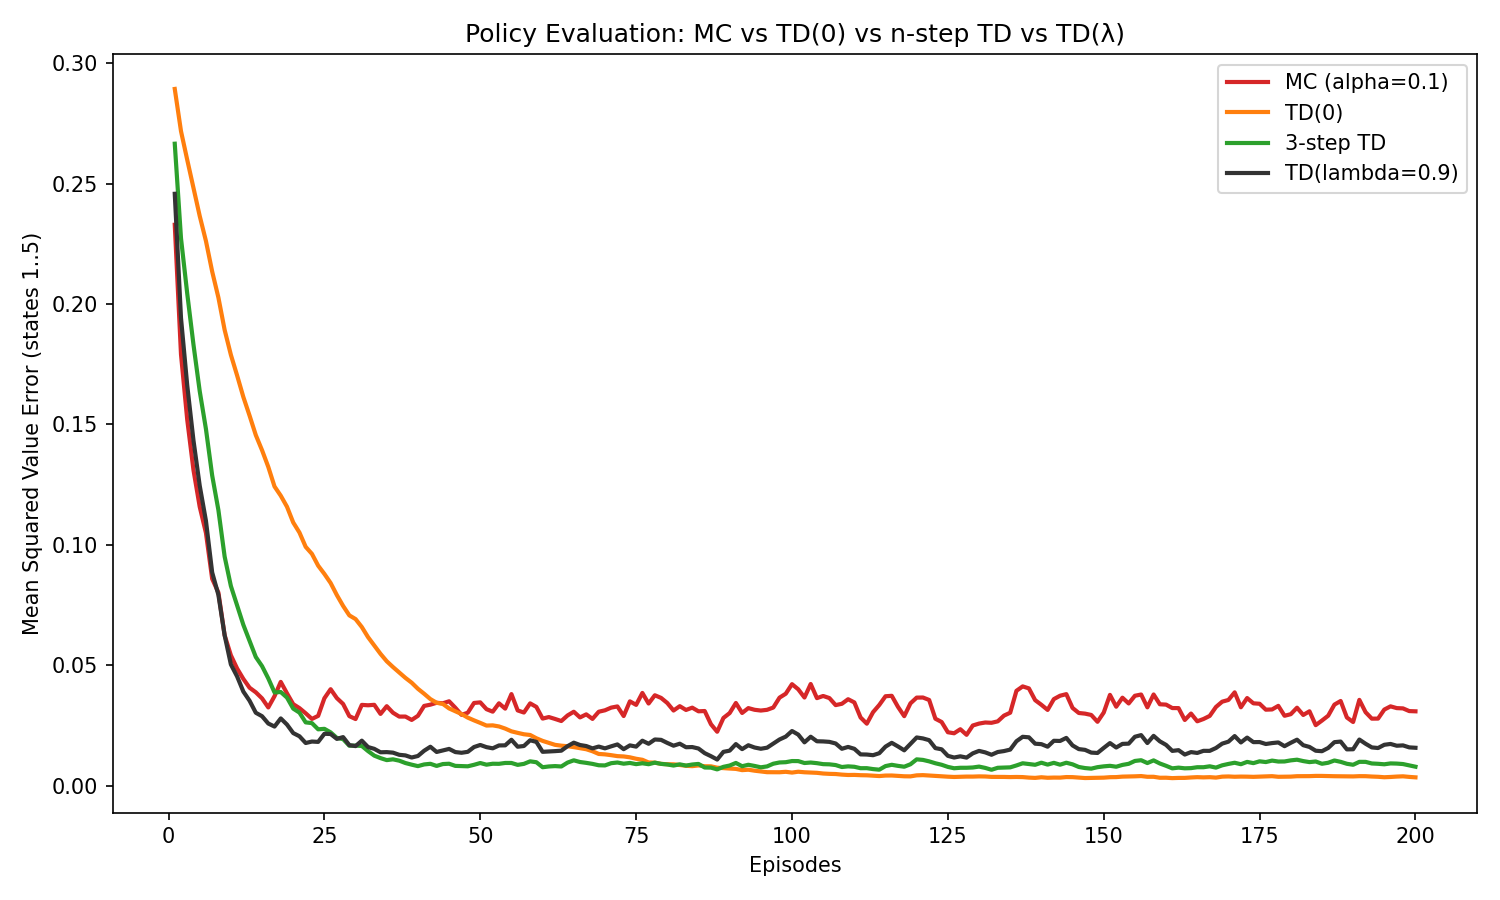
\includegraphics[width=0.9\linewidth]{images/Value-RL/mc_td_comparison_constant_step} 

}

\caption{Policy Evaluation, MC versus TD Family, Fixed Step Size}\label{fig:policy-evaluation-random-walk-fixed-step-size}
\end{figure}

\textbf{Diminishing Step Sizes.}
We then use a diminishing step size for the TD family:
\begin{equation}
\alpha_t(s) \;=\; \frac{c}{\big(N_t(s)+t_0\big)^p}, 
\qquad \tfrac{1}{2} < p \le 1,
\label{eq:per-state-decay}
\end{equation}
where \(N_t(s)\) counts how many times \(V(s)\) has been updated up to time \(t\). A common choice is \(p=1\) with moderate \(c>0\) and \(t_0>0\).

Fig. \ref{fig:policy-evaluation-random-walk-diminishing-step-size} shows the MSE versus episodes for MC, TD(0), 3-step TD, and TD(\(\lambda\)) under the diminishing step-size. Observe that all algorithms converge to the true value function under the diminishing step size schedule.

\begin{figure}

{\centering 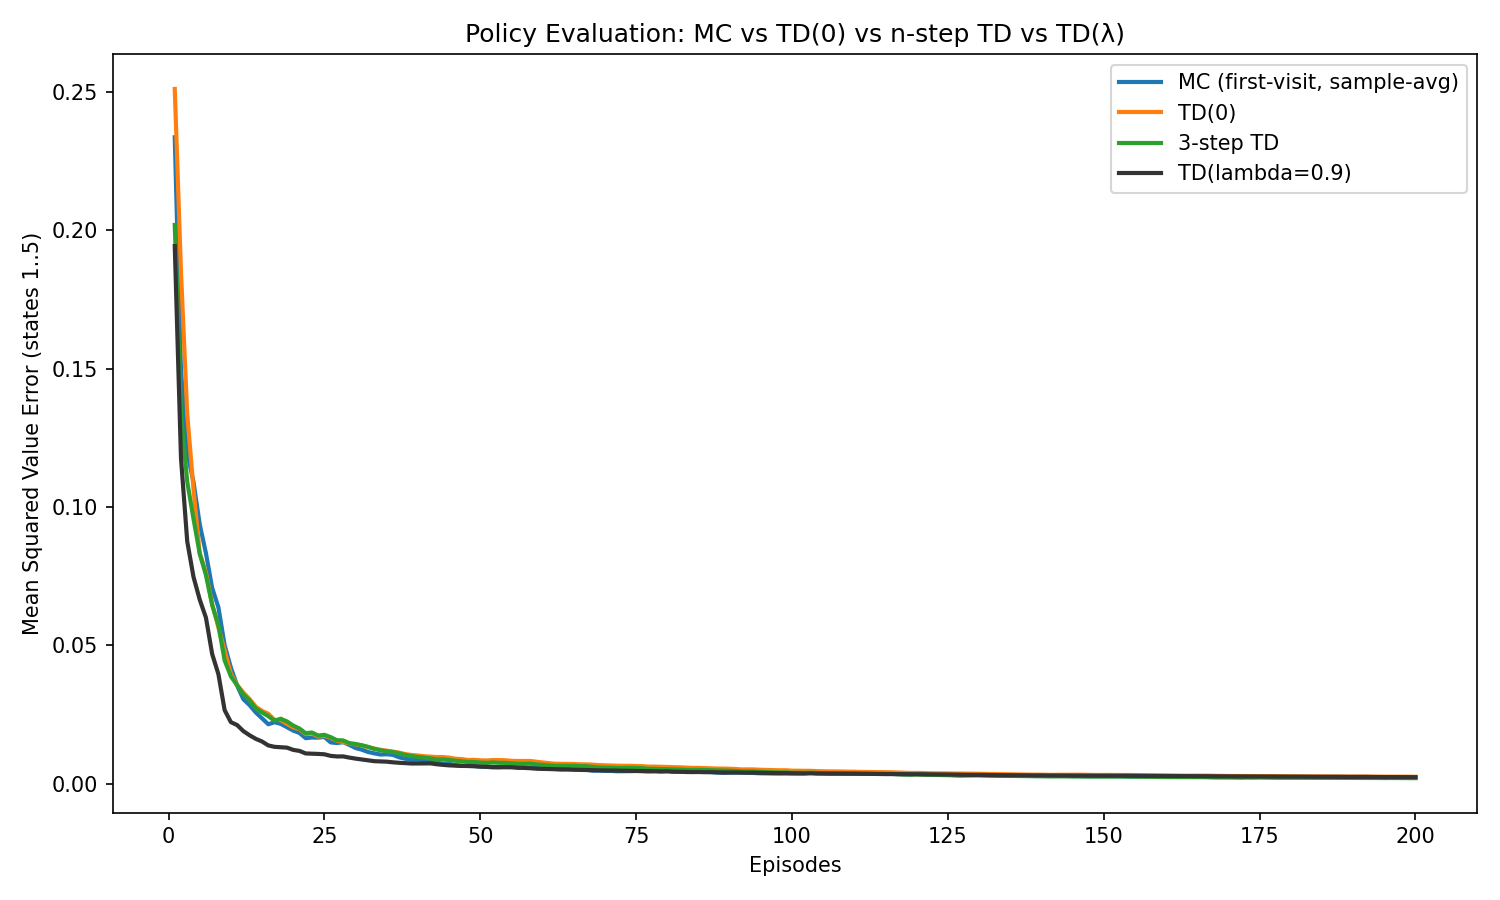
\includegraphics[width=0.9\linewidth]{images/Value-RL/mc_td_comparison_diminishing_step} 

}

\caption{Policy Evaluation, MC versus TD Family, Diminishing Step Size}\label{fig:policy-evaluation-random-walk-diminishing-step-size}
\end{figure}

You are encouraged to play with the parameters of these algorithms in the code \href{https://github.com/ComputationalRobotics/2025-ES-AM-158-LECTURE-CODE/blob/main/policy_evaluation_mc_td.py}{here}.
\end{example}

\subsection{Convergence Proof of TD Learning}\label{value-rl-convergence-td}

\textbf{Setup.} Consider a tabular MDP with finite state space \(\mathcal{S}\) and action space \(\mathcal{A}\), and a discount factor \(\gamma \in [0,1)\). Assume the reward function is bounded, for example, \(R(s,a) \in [0,1]\) for any \((s,a) \in \mathcal{S} \times \mathcal{A}\). Let \(\pi\) be a stochastic policy and \(V^\pi\) be the true value function associated with \(\pi\), the target we wish to estimate from interaction data. Denote
\[
\mathcal{F}_t = \sigma(s_0,a_0,r_0,\dots,s_{t-1},a_{t-1},r_{t-1}),
\]
as the \(\sigma\) algebra of all state-action-reward information up to time \(t-1\).

\textbf{TD(0) Update.} We maintain a tabular estimate \(V_t\) of the true value \(V^\pi\). On visiting \(s_t\) and observing \((s_t, a_t, r_t, s_{t+1})\), the TD(0) algorithm performs
\begin{equation}
V_{t+1}(s_t) = V_t(s_t) + \alpha_t(s_t) \delta_t,
\label{eq:TD0update-proof}
\end{equation}
where \(\delta_t\) is the TD error
\[
\delta_t = r_t + \gamma V_{t}(s_{t+1}) - V_t(s_t).
\]
The update \eqref{eq:TD0update-proof} only changes the value at \(s_t\), leaving the value at other states unchanged.

\textbf{Robbins--Monro Step Size.} We assume the step size \(\alpha\) satisfy the Robbins--Monro condition. That is, for any \(s \in \mathcal{S}\):
\[
\alpha_t(s) >0, \quad \sum_{t: s_t = s} \alpha_t(s) = \infty, \quad \sum_{t: s_t = s} \alpha^2_t(s) < \infty.
\]

\textbf{Stationary Distribution.}
Assume the Markov chain over \(\mathcal{S}\) induced by \(\pi\) is ergodic, then a unique stationary state distribution \(\mu^\pi\) exists and satisfy:
\begin{equation}
\mu^\pi(s') = \sum_{s \in \mathcal{S}} \mu^\pi(s) \left( \sum_{a \in \mathcal{A}}  \pi(a \mid s) P(s' \mid s, a) \right), \quad \forall s' \in \mathcal{S}.
\label{eq:StationaryDistribution-Tabular}
\end{equation}
If we denote
\begin{equation}
P^\pi(s' \mid s) = \sum_{a \in \mathcal{A}} \pi(a \mid s) P(s' \mid s,a),
\label{eq:TabularStateOnlyTransition}
\end{equation}
as the \(\pi\)-induced state-only transition dynamics, then condition \eqref{eq:StationaryDistribution-Tabular} is equivalent to
\begin{equation}
\mu^\pi(s') = \sum_{s \in \mathcal{S}} \mu^\pi(s) P^\pi (s' \mid s), \quad \forall s' \in \mathcal{S}.
\label{eq:StationaryDistribution-Tabular-State-Only}
\end{equation}

See \eqref{eq:StationaryDistribution-definition} for a generalization to continuous MDP.

\textbf{Bellman Operator.} For any \(V:\mathcal S\to\mathbb R\), define the Bellman operator associated with \(\pi\) as \(T^\pi V:\mathcal S\to\mathbb R\) by
\begin{equation}
(T^\pi V)(s)\;=\;\sum_{a\in\mathcal A}\pi(a\mid s)\sum_{s'\in\mathcal S} P(s'\mid s,a)\,\Big( R(s,a)+\gamma\,V(s')\Big).
\label{eq:BellmanOperatorRestate-TDConvergenceProof}
\end{equation}
We know that the operator \(T^\pi\) is a \(\gamma\)-contraction in \(\|\cdot\|_\infty\). Hence it has a unique fixed point \(V^\pi\) satisfying \(V^\pi=T^\pi V^\pi\).

The following theorem states the almost sure convergence of TD learning iterates to the true value function.

\begin{theorem}[TD(0) Convergence (Tabular)]
\protect\hypertarget{thm:TD0ConvergenceTabular}{}\label{thm:TD0ConvergenceTabular}Under the tabular MDP setup and assumptions above, the TD(0) iterates \(V_t\) generated by \eqref{eq:TD0update-proof} converge almost surely to \(V^\pi\).
\end{theorem}

To prove this theorem, we need the following two lemmas.

\begin{lemma}[Robbins-Siegmund Lemma]
\protect\hypertarget{lem:RobbinsSiegmund}{}\label{lem:RobbinsSiegmund}Let \((X_t)_{t\ge 0}\) be nonnegative and adapted to \((\mathcal F_t)\). Suppose there exist nonnegative \((\beta_t),(\gamma_t),(\xi_t)\) with \(\sum_t \gamma_t<\infty\) and \(\sum_t \xi_t<\infty\) such that
\[
\mathbb E[X_{t+1}\mid \mathcal F_t]\;\le\;(1+\gamma_t)X_t\;-\;\beta_t\;+\;\xi_t\qquad\text{almost surely}
\]
Then \(X_t\) converges almost surely to a finite random variable and \(\sum_t \beta_t<\infty\) almost surely.
\end{lemma}

This lemma is from \citep{robbins1971convergence}.

\begin{lemma}
\protect\hypertarget{lem:TDConvergenceLemma}{}\label{lem:TDConvergenceLemma}Let \(\mu^\pi\) be the stationary distribution in \eqref{eq:StationaryDistribution-Tabular-State-Only}, \(D=\mathrm{diag}(\mu^\pi)\), and \(w:=V-V^\pi\). Then
\[
\langle w,\,D\,(T^\pi V - V)\rangle\;\le\;-(1-\gamma)\,\|w\|_D^2,
\]
where \(\langle x,y\rangle=x^\top y\) and \(\|w\|_D^2=\sum_s \mu^\pi(s)\,w(s)^2\).
\end{lemma}

\begin{proof}
First, for any two value functions \(V, U \in \mathbb{R}^{|\mathcal{S}|}\), we have
\[
(T^\pi V)(s) - (T^\pi U)(s) = \gamma \sum_{a} \pi(a \mid s) \sum_{s'} P(s' \mid s,a) (V(s') - U(s)').
\]
Therefore,
\[
T^\pi V - T^\pi U = \gamma \widetilde P (V - U),
\]
with
\begin{equation}
(\widetilde P u)(s):=\sum_a\pi(a\mid s)\sum_{s'}P(s'\mid s,a)\,u(s').
\label{eq:def-tilde-P}
\end{equation}
With this, we can write
\begin{equation}
\begin{split}
T^\pi V - V & = T^\pi V - V^\pi + V^\pi - V \\
& = T^\pi V - T^\pi V^\pi - ( V - V^\pi ) \\
& = \gamma \widetilde P (V - V^\pi) - ( V - V^\pi ) \\
& = (\gamma \widetilde P - I) ( V - V^\pi ) \\
& = (\gamma \widetilde P - I) w.
\end{split}
\end{equation}
Thus,
\begin{equation}
\langle w, D(T^\pi V - V)\rangle
= -\,w^\top D\,(I-\gamma \widetilde P)\,w
= -\|w\|_D^2 + \gamma\,\langle w, D\,\widetilde P w\rangle.
\label{eq:InnerProductInequality}
\end{equation}

Next, we prove \(\langle w, D\widetilde P w\rangle\le \|w\|_D^2\).

\begin{itemize}
\item
  First, we show \(\|\widetilde P w\|_D\le \|w\|_D\). For any state \(s \in \mathcal{S}\), from \eqref{eq:def-tilde-P}, we have
  \[
  (\widetilde P w)(s) = \sum_{s'} P^\pi (s' \mid s) w(s'),
  \]
  where \(P^\pi(s' \mid s)\) is the \(\pi\)-induced state-only transition in \eqref{eq:TabularStateOnlyTransition}. Since \(P^\pi(\cdot \mid s)\) is a probability distribution, and \(x \mapsto x^2\) is convex, we have
  \[
  ((\widetilde P w)(s))^2 = \left( \sum_{s'} P^\pi (s' \mid s) w(s') \right)^2 \leq \sum_{s'} P^\pi (s' \mid s) w^2(s').
  \]
  Therefore, we have
  \begin{equation}
  \begin{split}
  \Vert \widetilde P w \Vert_D^2 & = \sum_s \mu^{\pi}(s) ((\widetilde P w)(s))^2 \\
  & \leq \sum_s \mu^{\pi}(s) \left( \sum_{s'} P^\pi (s' \mid s) w^2(s') \right) \\
  & = \sum_{s'} \left( \sum_{s} \mu^\pi(s) P^\pi(s' \mid s) \right) w^2(s') \\
  & = \sum_{s'} \mu^\pi (s') w^2 (s') = \Vert w \Vert_D^2.
  \end{split}
  \end{equation}
  where the second-from-last equality holds because \(\mu^\pi\) is the stationary distribution and satisfies \eqref{eq:StationaryDistribution-Tabular-State-Only}.
\item
  Second, we write
  \[
  \langle w, D\widetilde P w\rangle = \langle D^{0.5} w, D^{0.5} \widetilde P w \rangle \leq \Vert D^{0.5} w \Vert \cdot \Vert D^{0.5} \widetilde P w \Vert = \Vert w \Vert_D \cdot \Vert \widetilde P w \Vert_D \leq \Vert w \Vert_D^2.
  \]
\end{itemize}

Plugging this back to \eqref{eq:InnerProductInequality}, we obtain
\[
\langle w, D(T^\pi V - V) \rangle \leq - \Vert w \Vert_D^2 + \gamma \Vert w \Vert_D^2,
\]
proving the desired result in the lemma.
\end{proof}

We are now ready to prove Theorem \ref{thm:TD0ConvergenceTabular}.

\begin{proof}
\textbf{Step 1 (TD as stochastic approximation).} For the TD error
\[
\delta_t=r_{t}+\gamma V_t(s_{t+1})-V_t(s_t),
\]
we have the conditional expectation
\[
\mathbb E[\delta_t\mid \mathcal F_t, s_t]
=\sum_{a}\pi(a\mid s_t)\sum_{s'}P(s'\mid s_t,a)\Big(R(s_t,a)+\gamma V_t(s')\Big)-V_t(s_t)
=\big(T^\pi V_t - V_t\big)(s_t).
\]
Define the ``noise'':
\[
\eta_{t+1}:=\delta_t-\mathbb E[\delta_t\mid \mathcal F_t,s_t].
\]
Then \(\mathbb E[\eta_{t+1}\mid \mathcal F_t,s_t]=0\) and the TD update is equivalent to
\begin{equation}
V_{t+1}(s_t)=V_t(s_t)+\alpha_t(s_t)\Big( \big(T^\pi V_t - V_t\big)(s_t) + \eta_{t+1}\Big),
\label{eq:TDStochasticApproximation}
\end{equation}
while learving all other coordinates unchanged. Because rewards are uniformly bounded, we know that \(V_t\) remains bounded. Hence, \(\mathbb E[\eta_{t+1}^2\mid \mathcal F_t, s_t]\) is uniformly bounded. Equation \eqref{eq:TDStochasticApproximation} shows that the TD update can be seen as a stochastic approximation to the Bellman operator \eqref{eq:BellmanOperatorRestate-TDConvergenceProof}.

\textbf{Step 2 (Lyapunov drift).} Let \(D=\mathrm{diag}(\mu^\pi)\), a diagonal matrix whose diagonal entries are the probabilities in \(\mu^\pi\).
Define the Lyapunov function
\[
\mathcal L(V)=\frac{1}{2} \|V-V^\pi\|_D^2=\frac{1}{2} \sum_s \mu^\pi(s)\,\big(V(s)-V^\pi(s)\big)^2.
\]
Let \(w_t:=V_t - V^\pi\). Since only the \(s_t\)-coordinate changes at time \(t\), we have
\begin{equation}
\begin{split}
\mathcal L(V_{t+1})-\mathcal L(V_t)
&=\frac{1}{2} \mu^\pi(s_t)\Big(( \underbrace{V_t(s_t)+\alpha_t\delta_t}_{V_{t+1}(s_t)} - V^\pi(s_t) )^2 -(V_t(s_t)-V^\pi(s_t))^2\Big)\\
&= \mu^\pi(s_t)\,\alpha_t\,\delta_t\,w_t(s_t)\;+\;\frac{1}{2} \mu^\pi(s_t)\,\alpha_t^2\,\delta_t^{\,2}.
\end{split}
\label{eq:DifferenceBetweenLyapunov}
\end{equation}
Define \(g_t := T^\pi V_t - V_t\). Taking conditional expectation given \(\mathcal F_t\) and i.i.d. \(s_t\sim \mu^\pi\),
\begin{equation}
\begin{split}
\mathbb E\!\left[\mathcal L(V_{t+1})-\mathcal L(V_t)\mid \mathcal F_t\right]
&= \alpha_t\,\mathbb E\!\left[\mu^\pi(s_t)\,w_t(s_t)\,g_t(s_t)\mid \mathcal F_t\right]
+ \frac{1}{2} \alpha_t^2\,\mathbb E\!\left[\mu^\pi(s_t)\,\delta_t^{\,2}\mid \mathcal F_t\right]\\
&= \alpha_t\,\sum_s \mu^\pi(s)\,w_t(s)\,g_t(s) \;+\; \frac{1}{2} \alpha_t^2\,C_t,
\end{split}
\label{eq:DifferenceBetweenLyapunov-ConditionalExpectation}
\end{equation}
where \(C_t:=\mathbb E\!\left[\mu^\pi(s_t)\,\delta_t^{\,2}\mid \mathcal F_t\right]\) is finite because rewards are bounded and \(V_t\) stays bounded. Assume \(C_t \leq C\).

At the same time, by Lemma \ref{lem:TDConvergenceLemma}
\[
\sum_s \mu^\pi(s)\,w_t(s)\,g_t(s)
=\langle w_t, D g_t\rangle
\le -(1-\gamma)\,\|w_t\|_D^2.
\]
Plugging into \eqref{eq:DifferenceBetweenLyapunov-ConditionalExpectation} yields
\begin{equation}
\mathbb E\!\left[\mathcal L(V_{t+1})\mid \mathcal F_t\right]
\;\le\;
\mathcal L(V_t)\;-\;\alpha_t\,(1-\gamma)\,\|w_t\|_D^2\;+\;\frac{1}{2} \alpha_t^2\,C.
\label{eq:TD0ConvergenceProof-RS-Form}
\end{equation}
This is in Robbins--Siegmund form with
\[
X_t:=\mathcal L(V_t),\qquad
\beta_t:=(1-\gamma)\,\alpha_t\,\|w_t\|_D^2,\qquad
\gamma_t:=0,\qquad
\xi_t:=\frac{1}{2} C\,\alpha_t^2.
\]
We have \(\sum_t \xi_t<\infty\) by \(\sum_t \alpha_t^2<\infty\). Therefore \(X_t\) converges a.s. and \(\sum_t \beta_t<\infty\) a.s., which implies \(\sum_t \alpha_t \|w_t\|_D^2<\infty\). Since \(\sum_t \alpha_t=\infty\), it must be that \(\liminf_t \|w_t\|_D=0\).\\
Finally, using \eqref{eq:TD0ConvergenceProof-RS-Form} again and the continuity of the drift, one shows that any subsequential limit of \(V_t\) must satisfy \(T^\pi V - V=0\); by uniqueness of the fixed point, the only possible limit is \(V^\pi\). Hence \(V_t\to V^\pi\) almost surely.
\end{proof}

\subsection{On-Policy Control}\label{on-policy-control}

Monte Carlo (MC) estimation and the TD family evaluate policies directly from interaction---no model required. We now turn evaluation into control via generalized policy iteration (GPI): repeatedly (i) evaluate the current policy from data and (ii) improve it by acting greedily with respect to the new estimates. We first cover on-policy control methods, which estimate and improve the same (typically \(\varepsilon\)-greedy) policy, and then off-policy methods, which learn about a target policy while behaving with a different one.

\subsubsection{Monte Carlo Control}\label{monte-carlo-control}

\textbf{High-level Intuition.}

\begin{itemize}
\item
  \textbf{Goal.} Learn an (approximately) optimal policy by alternating \emph{policy evaluation} and \emph{policy improvement} using only sampled episodes.
\item
  \textbf{Why action-values?} Estimating \(Q^\pi(s,a)\) lets us improve the policy \emph{without a model} by choosing ``\(\arg\max_a Q(s,a)\)''.
\item
  \textbf{Exploration.} Pure greedy improvement can get stuck. MC control keeps the policy \emph{\(\varepsilon\)-soft} (e.g., \(\varepsilon\)-greedy) so that every action has nonzero probability and all state-action pairs continue to be sampled. An \(\varepsilon\)-soft policy is one that never rules out any action: in every state \(s\), each action \(a\) gets at least a small fraction of probability. Formally, in the tabular setup, we have that a policy \(\pi\) is \(\varepsilon\)-soft if and only if
  \begin{equation}
  \forall s, \forall a: \quad \pi(a \mid s) \geq \frac{\varepsilon}{|\mathcal{A}(s)|}, \quad \varepsilon \in (0,1],
  \label{eq:epsilon-soft-policy}
  \end{equation}
  where \(\mathcal{A}(s)\) denotes the set of actions the agent can select at state \(s\).
\item
  \textbf{Coverage mechanisms.} Classic guarantees use either:

  \begin{enumerate}
  \def\labelenumi{\arabic{enumi})}
  \tightlist
  \item
    \textbf{Exploring starts (ES):} start each episode from a randomly chosen \((s,a)\) with nonzero probability; or\\
  \item
    \textbf{\(\varepsilon\)-soft / GLIE (Greedy in the Limit with Infinite Exploration):} use \(\varepsilon\)-greedy behavior with \(\varepsilon_t \downarrow 0\) so every \((s,a)\) is visited infinitely often while the policy becomes greedy in the limit.
  \end{enumerate}
\end{itemize}

\textbf{Algorithmic Form.}
We maintain tabular action-value estimates \(Q(s,a)\) and an \emph{\(\varepsilon\)-soft} policy \(\pi\) (\(\varepsilon\)-greedy w.r.t. \(Q\)). After each episode we update \(Q\) from \emph{empirical returns} and then improve \(\pi\).

\textbf{Return from time \(t\):}
\[
g_t = r_t + \gamma r_{t+1} + \dots + \gamma^{T-t} r_T = \sum_{k=0}^{T-t} \gamma^{k} r_{t+k}.
\]

\textbf{First-visit MC update (common choice):}
\begin{equation}
Q(s_t,a_t) \;\leftarrow\; Q(s_t,a_t) + \alpha_{N(s_t,a_t)}\!\left(g_t - Q(s_t,a_t)\right),
\label{eq:MCControl-QUpdate}
\end{equation}
applied only on the first occurrence of \((s_t,a_t)\) in the episode. \emph{Sample-average} learning uses \(\alpha_n = 1/n\) per pair; more generally, use diminishing stepsizes.

\textbf{Policy improvement (\(\varepsilon\)-greedy):}
\begin{equation}
\pi(a|s) \;=\;
\begin{cases}
1-\varepsilon + \dfrac{\varepsilon}{|\mathcal{A}(s)|}, & a \in \arg\max_{a'} Q(s,a'), \\
\dfrac{\varepsilon}{|\mathcal{A}(s)|}, & \text{otherwise}.
\end{cases}
\label{eq:MCControl-PI}
\end{equation}

\textbf{Theoretical Guarantees.}

Assume a tabular episodic MDP and \(\gamma \in [0,1)\).

\begin{itemize}
\item
  \textbf{Convergence with Exploring Starts.} If every state--action pair has nonzero probability of being the \emph{first} pair of an episode (using ES), and each \(Q(s,a)\) is updated toward the true mean return from \((s,a)\) (e.g., via sample averages), then repeated policy evaluation and greedy improvement converge with probability 1 to an optimal deterministic policy. (If one uses an \(\varepsilon\)-greedy improvement, then it converges to an optimal \(\varepsilon\)-soft policy.)
\item
  \textbf{Convergence with \(\varepsilon\)-soft GLIE behavior.} If the behavior policy is GLIE---every \((s,a)\) is visited infinitely often and \(\epsilon_t \to 0\)---and the stepsizes for each \((s,a)\) satisfy the Robbins--Monro conditions \(\sum_{t} \alpha_t(s,a) = \infty,\sum_{t} \alpha_t(s,a)^2 < \infty\), then \(Q(s,a)\) converges to \(Q^\star(s,a)\) for all pairs visited infinitely often, and the \(\varepsilon\)-greedy policy converges almost surely to an optimal policy.
\end{itemize}

\begin{remark}
\textbf{Unbiased but high-variance.} MC targets \(g_t\) are unbiased estimates of action values under the current policy, but can have high variance---especially for long horizons---so convergence can be slower than TD methods. Keeping \(\varepsilon>0\) ensures exploration but limits asymptotic optimality to the best \(\varepsilon\)-soft policy; hence \(\varepsilon_t \downarrow 0\) (GLIE) is recommended for optimality.
\end{remark}

\subsubsection{SARSA (On-Policy TD Control)}\label{sarsa-on-policy-td-control}

\textbf{High-level Intuition.}

\begin{itemize}
\tightlist
\item
  \textbf{Goal.} Turn evaluation into control by updating action values online and improving the same policy that generates data.
\item
  \textbf{Key idea.} Replace Monte Carlo returns with a bootstrapped target. After taking action \(a_t\) in state \(s_t\) and observing \(r_{t}, s_{t+1}\), sample the next action \(a_{t+1}\) from the current policy and update toward \(r_{t} + \gamma Q(s_{t+1}, a_{t+1})\).
\item
  \textbf{On-policy nature.} SARSA evaluates the behavior policy itself, typically an \(\varepsilon\)-greedy policy w.r.t. \(Q\).
\item
  \textbf{Exploration.} Use \(\varepsilon\)-soft behavior so every action keeps nonzero probability. For optimality, let \(\varepsilon_t \downarrow 0\) to obtain GLIE (Greedy in the Limit with Infinite Exploration).
\end{itemize}

\textbf{Algorithmic Form.}

Let \(Q\) be a tabular action-value function and \(\pi_t\) be \(\varepsilon_t\)-greedy w.r.t. \(Q_t\).

\textbf{TD target and error:}
\begin{equation}
y_t = r_{t} + \gamma Q(s_{t+1}, a_{t+1}), \qquad
\delta_t = y_t - Q(s_t, a_t).
\label{eq:SARSA-TDTarget}
\end{equation}

\textbf{SARSA update (one-step):}
\begin{equation}
Q(s_t, a_t) \leftarrow Q(s_t, a_t) + \alpha_t(s_t,a_t)\, \delta_t.
\label{eq:SARSA-QUpdate}
\end{equation}

\textbf{\(\varepsilon\)-greedy policy improvement:}
\begin{equation}
\pi_{t+1}(a\mid s) =
\begin{cases}
1-\varepsilon_{t+1} + \dfrac{\varepsilon_{t+1}}{|\mathcal A(s)|}, & a \in \arg\max_{a'} Q_{t+1}(s,a'),\\
\dfrac{\varepsilon_{t+1}}{|\mathcal A(s)|}, & \text{otherwise.}
\end{cases}
\label{eq:SARSA-PolicyUpdate}
\end{equation}

\textbf{Variants.}

\begin{itemize}
\item
  \textbf{Expected SARSA} replaces the sampled \(a_{t+1}\) by its expectation under \(\pi_t\) for lower variance:
  \begin{equation}
  y_t = r_{t} + \gamma \sum_a \pi_t(a\mid s_{t+1}) Q(s_{t+1}, a).
  \label{eq:ExpectedSARSA-Target}
  \end{equation}
\item
  \textbf{\(n\)-step SARSA} and \textbf{SARSA(\(\lambda\))} blend multi-step targets; these trade bias and variance similarly to MC vs TD.
\end{itemize}

\textbf{Convergence Guarantees.}

Assume a finite MDP, \(\gamma \in [0,1)\), asynchronous updates, and that each state--action pair is visited infinitely often.

\begin{itemize}
\tightlist
\item
  \textbf{GLIE convergence to optimal policy.} If the behavior is GLIE, i.e., \(\varepsilon_t \downarrow 0\) while ensuring infinite exploration, and stepsizes satisfy the Robbins--Monro conditions, then \(Q_t \to Q^\star\) almost surely and the \(\varepsilon_t\)-greedy behavior becomes greedy in the limit, yielding an optimal policy almost surely.
\end{itemize}

\subsection{Off-Policy Control}\label{off-policy-control}

Off-policy methods learn about a \emph{target} policy \(\pi\) while following a (potentially different) \emph{behavior} policy \(b\) to gather data. This decoupling is useful when:

\begin{itemize}
\item
  you want to \emph{reuse logged data} collected by some \(b\) (e.g., a rule-based controller or a past system),
\item
  you need \emph{safer exploration} by restricting behavior \(b\) while aiming to evaluate or improve a different \(\pi\),
\item
  you want to learn about the \emph{greedy} policy without executing it, which motivates algorithms like Q-learning.
\end{itemize}

In this section we first cover off-policy policy evaluation with \emph{importance sampling}, then show how it can be used to construct an off-policy \emph{Monte Carlo control} scheme in the tabular case. Finally, we present Q-learning.

\subsubsection{Importance Sampling for Policy Evaluation}\label{importance-sampling-for-policy-evaluation}

\textbf{Motivation.} Suppose we have episodes generated by a behavior policy \(b\), but we want the value of a different target policy \(\pi\). For a state value this is \(V^\pi(s) = \mathbb{E}_\pi[g_t \mid s_t=s]\), and for action values \(Q^\pi(s,a) = \mathbb{E}_\pi[g_t \mid s_t=s, a_t=a]\), where
\[
g_t = \sum_{k=0}^{T-t} \gamma^{k} r_{t+k}.
\]
Because the data come from \(b\), the naive sample average is biased. Importance sampling (IS) reweights returns so that expectations under \(b\) equal those under \(\pi\).

A basic \emph{support condition} is required:
\begin{equation}
\text{If } \pi(a\mid s) > 0 \text{ then } b(a\mid s) > 0 \quad \text{for all visited } (s,a).
\label{eq:IS-SupportCondition}
\end{equation}
This ensures that \(\pi\) is absolutely continuous with respect to \(b\) on the experienced trajectories.

\textbf{Importance Sampling (episode-wise).} Consider a trajectory starting at time \(t\):
\[
\tau_t = (s_t, a_t, r_t, s_{t+1}, a_{t+1}, \dots, s_{T-1}, a_{T-1}, r_{T-1}, s_T).
\]
The probability of observing this trajectory conditioned on \(s_t = s\), under policy \(\pi\), is
\[
\mathbb{P}_{\pi}[\tau_t \mid s_t = s] = \pi(a_t \mid s_t) P(s_{t+1} \mid s_t, a_t) \pi(a_{t+1} \mid s_{t+1}) \cdots \pi(a_{T-1} \mid s_{T-1}) P(s_T \mid s_{T-1}, a_{T-1}).
\]
The probability of observing the same trajectory conditioned on \(s_t = s\), under policy \(b\), is
\[
\mathbb{P}_{b}[\tau_t \mid s_t = s] = b(a_t \mid s_t) P(s_{t+1} \mid s_t, a_t) b(a_{t+1} \mid s_{t+1}) \cdots b(a_{T-1} \mid s_{T-1}) P(s_T \mid s_{T-1}, a_{T-1}).
\]
Since the return \(g_t\) is a deterministic function of \(\tau_t\), i.e., applying the reward function \(R\) to state-action pairs, we have that
\begin{equation}
\begin{split}
V^\pi (s) & = \mathbb{E}_{\pi}[g_t \mid s_t = s] = \sum_{\tau_t} g_t \mathbb{P}_\pi [\tau_t \mid s_t = s] \\
& = \sum_{\tau_t} g_t \mathbb{P}_b[\tau_t \mid s_t = s] \left(\frac{\mathbb{P}_\pi [\tau_t \mid s_t = s]}{\mathbb{P}_b[\tau_t \mid s_t = s]} \right) \\
& = \sum_{\tau_t} \left( \frac{\pi(a_t \mid s_t) \pi(a_{t+1} \mid s_{t+1}) \cdots \pi(a_{T-1} \mid s_{T-1}) }{b(a_t \mid s_t)  b(a_{t+1} \mid s_{t+1}) \cdots b(a_{T-1} \mid s_{T-1})} \right) g_t \mathbb{P}_b [\tau_t \mid s_t = s]
\end{split}
\label{eq:IS-Trajectory-LikelihoodRatio}
\end{equation}
Therefore, define the \emph{likelihood ratio}
\begin{equation}
\rho_{t:T-1} = \prod_{k=t}^{T-1} \frac{\pi(a_k \mid s_k)}{b(a_k \mid s_k)},
\label{eq:IS-LikelihoodRatio}
\end{equation}
we have
\begin{equation}
V^\pi(s) = \mathbb{E}_b\left[\rho_{t:T-1} g_t \mid s_t=s\right]. 
\label{eq:IS-Value}
\end{equation}
Similarly, we have
\begin{equation}
Q^\pi(s,a) =  \mathbb{E}_b\!\left[\rho_{t:T-1} g_t \mid s_t=s, a_t=a\right].
\label{eq:IS-ActionValue}
\end{equation}
Given \(n\) episodes, the ordinary IS estimator for \(Q^\pi\) at the first visit of \((s,a)\) is
\[
\hat Q_n^{\text{IS}}(s,a) = \frac{1}{N_n(s,a)} \sum_{i=1}^n \mathbf{1}\{(s,a)\text{ visited}\}\, \rho_{t_i:T_i-1}^{(i)}\, g_{t_i}^{(i)},
\]
where \(N_n(s,a)\) counts the number of first visits of \((s,a)\). In words, to estimate the \(Q\) value of the target policy \(\pi\) using trajectories of the behavior policy \(b\), we need to reweight the return \(g_t\) by the likelihood ratio \(\rho_{t:T-1}\). Note that the likelihood ratio does not require knowledge about the transition dynamics.

\textbf{Algorithmic Form: Off-policy Monte Carlo Policy Evaluation.}

\textbf{Input:} behavior \(b\), target \(\pi\), episodes from \(b\)\\
\textbf{For each episode} \((s_0,a_0,r_0,s_1,\dots,s_{T-1},a_{T-1},r_{T-1},s_T)\):

\begin{enumerate}
\def\labelenumi{\arabic{enumi}.}
\item
  For \(t=T-1,\dots,0\) compute episode-wise likelihood ratio \(\rho_{t:T-1}\) and return \(g_t\),
\item
  For first visits of \((s_t,a_t)\), update
  \[
  Q(s_t,a_t) \leftarrow Q(s_t,a_t) + \alpha_{N(s_t,a_t)}\big(\rho_{t:T-1} g_t - Q(s_t,a_t)\big).
  \]
  Use sample averages \(\alpha_n=1/n\) or Robbins-Monro stepsizes.
\end{enumerate}

\textbf{Guarantees.} Under the support condition and finite variance assumptions, ordinary IS is \emph{unbiased} and converges almost surely to \(Q^\pi\).

\subsubsection{Off-Policy Monte Carlo Control}\label{off-policy-monte-carlo-control}

\textbf{High-level Intuition.} We wish to improve a target policy \(\pi\) toward optimality while behaving with a different exploratory policy \(b\). We evaluate \(Q^\pi\) off-policy using IS on data from \(b\), then set \(\pi\) greedy with respect to the updated \(Q\). Keep \(b\) sufficiently exploratory (for coverage), for example \(\varepsilon\)-greedy with a fixed \(\varepsilon>0\) or a GLIE schedule.

\textbf{Algorithmic Form.}

\begin{enumerate}
\def\labelenumi{\arabic{enumi}.}
\item
  Initialize \(Q(s,a)\) arbitrarily. Set target \(\pi\) to be greedy w.r.t. \(Q\). Choose an exploratory behavior \(b\) that ensures coverage, e.g., \(\varepsilon\)-greedy w.r.t. \(Q\) with \(\varepsilon>0\).
\item
  Loop over iterations \(i=0,1,2,\dots\):

  \begin{enumerate}
  \def\labelenumii{\arabic{enumii}.}
  \tightlist
  \item
    Data collection under \(b\): generate a batch of episodes using \(b\).
  \item
    Off-policy evaluation of \(\pi\): for each episode, compute IS targets for first visits of \((s_t,a_t)\) and update \(Q\) using either ordinary IS
  \item
    Policy improvement: set for all states
    \[
    \pi_{i+1}(s) \in \arg\max_{a} Q(s,a).
    \]
  \item
    Optionally update \(b\) to remain exploratory, for example \(b\) \(\leftarrow\) \(\varepsilon\)-greedy w.r.t. \(Q\) with a chosen \(\varepsilon\) or a GLIE decay.
  \end{enumerate}
\end{enumerate}

\textbf{Convergence Guarantees.}

\begin{itemize}
\item
  \textbf{Evaluation step:} With the support condition and appropriate stepsizes, off-policy MC prediction converges almost surely to \(Q^\pi\) when using ordinary IS.
\item
  \textbf{Control in the batch GPI limit:} If each evaluation step produces estimates that converge to the exact \(Q^{\pi_i}\) before improvement, then by the policy improvement theorem the sequence of greedy target policies \(\pi_i\) converges to an optimal policy in finite MDPs.
\end{itemize}

\begin{remark}
\textbf{Choice of \(b\).} A common and simple choice is an \(\varepsilon\)-greedy behavior \(b\) w.r.t. current \(Q\) that maintains \(\varepsilon>0\) for coverage or uses GLIE so that \(\varepsilon_t \downarrow 0\) while all pairs are still visited infinitely often.
\end{remark}

\subsubsection{Q-Learning}\label{q-learning}

\textbf{High-Level Intuition.}

\begin{itemize}
\item
  \textbf{What it learns.} Q-Learning seeks the fixed point of the Bellman optimality operator
  \[
  (\mathcal T^\star Q)(s,a) = \mathbb E\big[ r_{t} + \gamma \max_{a'} Q(s_{t+1}, a') \mid s_t=s, a_t=a \big],
  \]
  whose unique fixed point is \(Q^\star\). Because \(\mathcal T^\star\) is a \(\gamma\)-contraction in \(\|\cdot\|_\infty\), repeatedly applying it converges to \(Q^\star\) in the tabular case.
\item
  \textbf{Why off-policy.} We can behave with any sufficiently exploratory policy \(b\) (e.g., \(\varepsilon\)-greedy w.r.t. current \(Q\)) but learn from the greedy target \(\max_{a'} Q(s',a')\). No importance sampling is needed.
\end{itemize}

\textbf{Algorithmic Form.} Let \(Q\) be a tabular action-value function. At each step observe a transition \((s_t, a_t, r_{t}, s_{t+1})\) generated by a behavior policy \(b_t\) (typically \(\varepsilon_t\)-greedy w.r.t. \(Q_t\)).

\begin{itemize}
\item
  \textbf{Target and TD error}
  \[
  y_t = r_{t} + \gamma \max_{a'} Q(s_{t+1}, a'), \qquad
  \delta_t = y_t - Q(s_t, a_t).
  \]
\item
  \textbf{Update}
  \[
  Q(s_t, a_t) \leftarrow Q(s_t, a_t) + \alpha_t(s_t,a_t)\, \delta_t.
  \]
\item
  \textbf{Behavior (exploration)}
  Use \(\varepsilon_t\)-greedy with \(\varepsilon_t\) decaying (GLIE) or any scheme that ensures each \((s,a)\) is updated infinitely often.
\end{itemize}

\textbf{Convergence.} In a finite MDP with \(\gamma \in [0,1)\), if each \((s,a)\) is updated infinitely often (sufficient exploration) and stepsizes satisfy Robbins-Monro conditions, then Q-Learning converges to \(Q^\star\) with probability 1.

\subsubsection{Double Q-Learning}\label{double-q-learning}

\textbf{Motivation.} Max operators tend to be optimistically biased when action values are noisy. Consider an example where in state \(s\) one can take two actions \(1\) and \(2\). The estimated Q function \(\hat{Q}(s, \cdot)\) has two values \(+1\) and \(-1\) with equal probability. In this case we have \(Q(s,1) = Q(s,2) = \mathbb{E}[\hat{Q}(s,\cdot)] = 0\). Therefore, \(\max Q(s,a) = 0\). However, the noisy estimated \(\hat{Q}(s,\cdot)\) has four outcomes with equal probabilities:
\[
(+1,-1), (+1,+1), (-1, +1), (-1,-1).
\]
Therefore, we have
\[
\mathbb{E}[\max_a \hat{Q}(s,a)] = \frac{1}{4} (1 + 1 + 1 -1) = 1/2 > \max_a Q(s,a),
\]
which overestimates the max \(Q\) value. In general, we have
\[
\mathbb{E}[\max_a \hat{Q}(s,a)] \geq \max_a \mathbb{E} [\hat{Q}(s,a)] = \max_a Q(s,a),
\]
where the estimates \(\hat{Q}\) are noisy (try to prove this on your own).
In Q-Learning the target
\[
y_t = r_{t} + \gamma \max_{a'} Q(s_{t+1}, a')
\]
can therefore overestimate action values and slow learning or push policies toward risky actions.

Double Q-Learning reduces this bias by decoupling selection from evaluation: maintain two independent estimators \(Q^A\) and \(Q^B\). Use one to select the greedy action and the other to evaluate it, and alternate which table you update. This weakens the statistical coupling that creates overestimation.

\textbf{Algorithmic Form.} Keep two tables \(Q^A, Q^B\). Use an \(\varepsilon\)-greedy behavior policy with respect to a combined estimate, e.g., \(Q^{\text{avg}}= \tfrac12(Q^A+Q^B)\) or \(Q^A+Q^B\).

At each step observe \((s_t, a_t, r_{t}, s_{t+1})\). With probability \(1/2\) update \(Q^A\), else update \(Q^B\).

\begin{itemize}
\item
  \textbf{Update \(Q^A\):}
  \[
  a^\star = \arg\max_{a'} Q^A(s_{t+1}, a'),\qquad
  y_t = r_{t} + \gamma\, Q^B(s_{t+1}, a^\star),
  \]
  \[
  Q^A(s_t, a_t) \leftarrow Q^A(s_t, a_t) + \alpha_t(s_t,a_t)\big[y_t - Q^A(s_t, a_t)\big].
  \]
\item
  \textbf{Update \(Q^B\):}
  \[
  a^\star = \arg\max_{a'} Q^B(s_{t+1}, a'),\qquad
  y_t = r_{t} + \gamma\, Q^A(s_{t+1}, a^\star),
  \]
  \[
  Q^B(s_t, a_t) \leftarrow Q^B(s_t, a_t) + \alpha_t(s_t,a_t)\big[y_t - Q^B(s_t, a_t)\big].
  \]
\item
  \textbf{Behavior policy (\(\varepsilon\)-greedy):} choose \(a_t \sim \varepsilon\)-greedy with respect to \(Q^{\text{avg}}(s_t,\cdot)\).
  A GLIE schedule \(\varepsilon_t \downarrow 0\) is standard.
\item
  \textbf{Acting and planning:} for greedy actions or plotting a single estimate, use \(Q^{\text{avg}} = \tfrac12(Q^A+Q^B)\).
\end{itemize}

\textbf{Convergence.}

\begin{itemize}
\tightlist
\item
  \textbf{Tabular setting.} In a finite MDP with \(\gamma \in [0,1)\), bounded rewards, sufficient exploration so that every \((s,a)\) is updated infinitely often, and Robbins--Monro stepsizes for each pair. Double Q-Learning converges with probability 1 to \(Q^\star\).
\end{itemize}

\begin{example}[Value-based RL for Grid World]
\protect\hypertarget{exm:GridWorldMCControl}{}\label{exm:GridWorldMCControl}

Consider the following \(5 \times 5\) grid with \((0,4)\) being the goal and the terminal state. At every state, the agent can take four actions: left, right, up, and down. There is a wall in the gray area shown in Fig. \ref{fig:grid-world}. Upon hitting the wall, the agent stays in the original cell. Every action incurs a reward of \(-1\). Once the agent arrives at the goal state, reward stays at 0.

\begin{figure}

{\centering 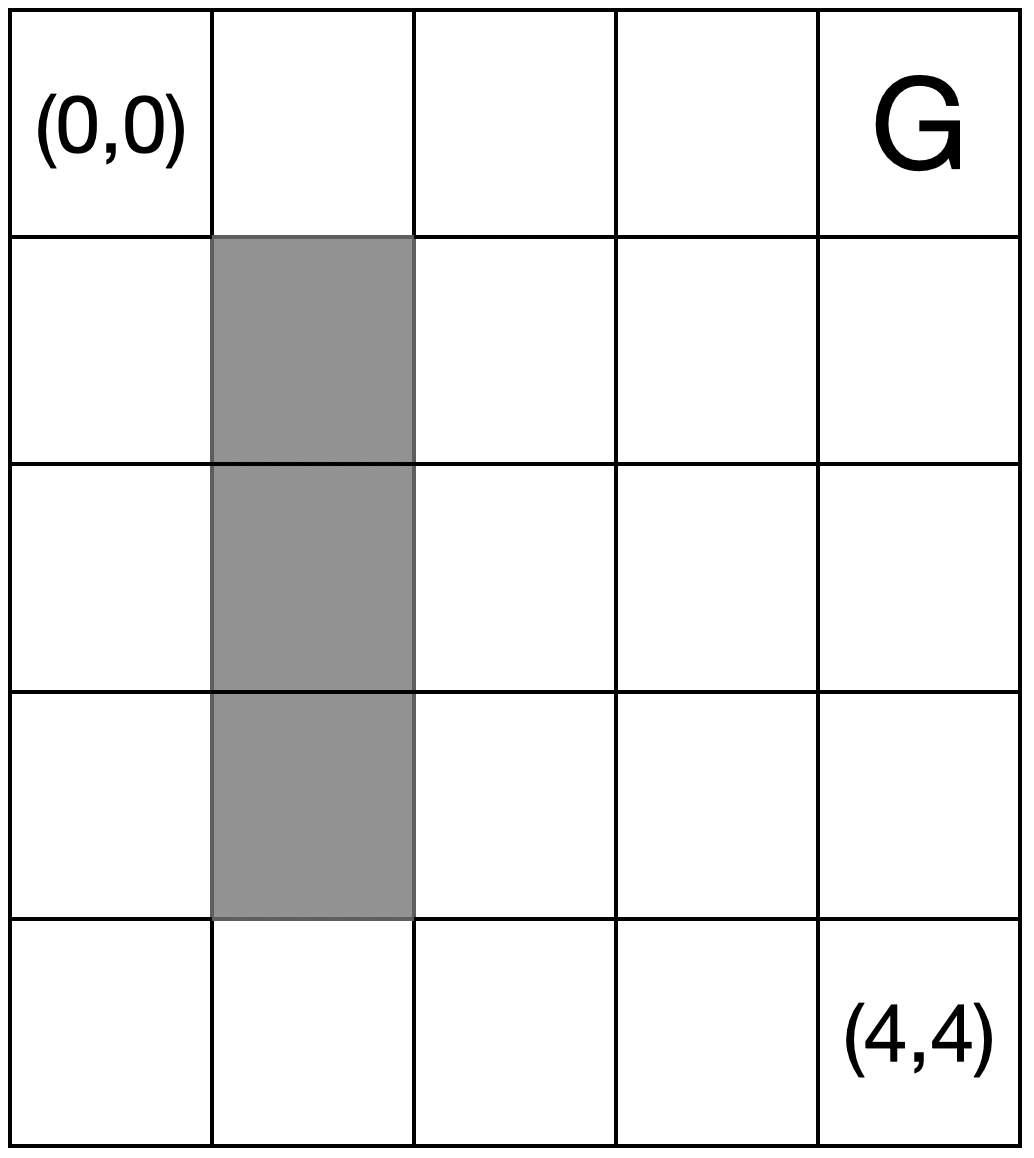
\includegraphics[width=0.4\linewidth]{images/Value-RL/grid-world} 

}

\caption{Grid World}\label{fig:grid-world}
\end{figure}

We run Generalized Policy Iteration (GPI) with Monte Carlo (on-policy), SARSA, Expected SARSA, Q-Learning, and Double Q-Learning on this problem with diminishing learning rates.

Fig. \ref{fig:grid-world-Q-convergence} plots the error between the estimated Q values (of different algorithms) and the ground-truth optimal Q value (obtained from value iteration with known transition dynamics). Except Monte Carlo control which converges slowly, the other methods converge fast.

\begin{figure}

{\centering 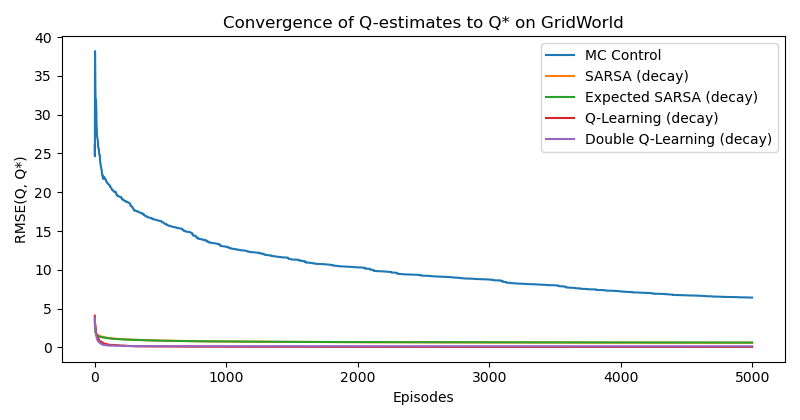
\includegraphics[width=0.9\linewidth]{images/Value-RL/Q-Value-Convergence} 

}

\caption{Convergence of Estimated Q Values.}\label{fig:grid-world-Q-convergence}
\end{figure}

From the final estimated Q value, we can extract a greedy policy, visualized below.

You can play with the code \href{https://github.com/ComputationalRobotics/2025-ES-AM-158-LECTURE-CODE/blob/main/GPI_GridWorld.py}{here}.

\begin{verbatim}
MC Control:
 > > > > G
^ # ^ ^ ^
v # ^ ^ ^
v # > ^ ^
> > > > ^
SARSA:
 > > > > G
^ # > > ^
^ # ^ ^ ^
^ # ^ ^ ^
> > ^ ^ ^
Expected SARSA:
 > > > > G
^ # > > ^
^ # ^ ^ ^
^ # > > ^
> > ^ ^ ^
Q-Learning:
 > > > > G
^ # ^ ^ ^
^ # ^ ^ ^
^ # ^ ^ ^
> > ^ ^ ^
Double Q-Learning:
 > > > > G
^ # > ^ ^
^ # > ^ ^
^ # ^ ^ ^
> > > > ^
\end{verbatim}

\end{example}

\section{Function Approximation}\label{function-approximation}

Many reinforcement learning problems have continuous state spaces--think of mechanical systems like robot arms, legged locomotion, drones, and autonomous vehicles. In these domains the state \(s\) (e.g., joint angles/velocities, poses) lives in \(\mathbb{R}^n\), which makes a tabular representation of the value functions impossible. In this case, we must approximate values with parameterized functions.

\subsection{Basics of Continuous MDP}\label{basics-of-continuous-mdp}

In a continuous MDP, at least one of the state space or the action space is a continuous space. Suppose \(\mathcal{S} \subseteq \mathbb{R}^n\) and \(\mathcal{A} \subseteq \mathbb{R}^{m}\) are both continuous spaces.

The environment kernel \(P(\cdot \mid s, a)\) is a Markov kernel from \(\mathcal{S} \times \mathcal{A}\) to \(\mathcal{S}\): for each state-action pair \((s,a)\), \(P(\cdot \mid s,a)\) is a probability measure on \(\mathcal{S}\). For each Borel set \(B \subseteq \mathcal{S}\), the map \((s,a) \mapsto P(B \mid s, a)\) is measurable. For example, \(P(\mathcal{S} \mid s, a) = 1\) for any \((s,a)\).

The policy kernel \(\pi(\cdot \mid s)\) is a stochastic kernel from \(\mathcal{S}\) to \(\mathcal{A}\): for each \(s\), \(\pi(\cdot \mid s)\) is a probability measure on \(\mathcal{A}\).

\textbf{Induced State-Transition Kernel.} For notational convenience, given a policy and the environment kernel \(P\), we define a state-only Markov kernel
\begin{equation}
P^\pi(B \mid s) := \int_{\mathcal{A}} P(B \mid s, a) \pi(da \mid s), \quad B \subseteq \mathcal{S}.
\label{eq:StateOnlyMarkovKernel}
\end{equation}
In words, \(P^\pi(B \mid s)\) measures the probability of landing at a set \(B\) starting from state \(s\), under all actions possible for the policy \(\pi\).

If densities exist, i.e., \(P(ds' \mid s, a) = p(s' \mid s, a) ds'\) and \(\pi(da \mid s) = \pi(a \mid s) da\), then,
\begin{equation}
p^\pi(s' \mid s) := \int_{\mathcal{A}} p(s' \mid s, a) \pi(a \mid s) da \quad\text{and}\quad P^{\pi}(d s' \mid s) = p^\pi(s' \mid s) ds'.
\label{eq:StateOnlyMarkovKernel-density}
\end{equation}

\textbf{Stationary State Distribution.} A probability measure \(\mu^\pi\) on \(\mathcal{S}\) is called \emph{stationary} for the state-transition kernel \(P^\pi\) if and only if
\begin{equation}
\mu^{\pi}(B) = \int_{\mathcal{S}} P^\pi(B \mid s) \mu^{\pi}(ds), \quad \forall B \subseteq \mathcal{S}.
\label{eq:StationaryDistribution-definition}
\end{equation}
If a density \(\mu^\pi(s)\) exists, then the above equation is the followng condition
\begin{equation}
\mu^{\pi}(s') = \int_{\mathcal{S}} p^\pi(s' \mid s) \mu^{\pi}(s) ds.
\label{eq:StationaryDistribution-definition-density}
\end{equation}
In words, the state distribution \(\mu^\pi\) does not change under the state-transition kernel \(P^\pi\) (e.g., if a state \(A\) has probability \(0.1\) of being visited at time \(t\), the probability of visiting \(A\) in the next time step remains \(0.1\), under policy \(\pi\)).
Under standard ergodicity assumptions, this stationary state distribution \(\mu^\pi\) exists and is unique (after sufficient steps, the initial state distribution does not matter and the state distribution follows \(\mu^\pi\)). Moreover, the empirical state distribution converge to \(\mu^\pi\).

\subsection{Policy Evaluation}\label{policy-evaluation-3}

For simplicity, let us first relax the state space to be a continuous space \(\mathcal{S} \subseteq \mathbb{R}^n\). We assume the action space \(\mathcal{A}\) is still finite with \(|\mathcal{A}|\) elements. We first consider the problem of policy evaluation, i.e., estimate the value functions associated with a policy \(\pi\) from interaction data with the environment.

\textbf{Bellman Consistency.} Given a policy \(\pi: \mathcal{S} \mapsto \Delta(\mathcal{A})\), its associated state-value function \(V^\pi\) must satisfy the following Bellman Consistency equation
\begin{equation}
V^{\pi}(s) = \sum_{a \in \mathcal{A}} \pi(a \mid s) \left[ R(s, a) + \gamma \int_{\mathcal{S}} V(s') P(d s' \mid s, a)  \right].
\label{eq:BellmanConsistencyContinuousStateFiniteAction}
\end{equation}
Notice that since \(\mathcal{S}\) is a continuous space, we need to replace ``\(\sum_{s' \in \mathcal{S}}\)'' with ``\(\int_{\mathcal{S}}\)''. If \(P(d s' \mid s, a)\) has a density \(p(s' \mid s, a)\), the above Bellman consistency equation also reads
\begin{equation}
V^{\pi}(s) = \sum_{a \in \mathcal{A}} \pi(a \mid s) \left[ R(s, a) + \gamma \int_{\mathcal{S}} V(s') p(s' \mid s, a) ds'  \right].
\label{eq:BellmanConsistencyContinuousStateFiniteAction-1}
\end{equation}

\textbf{Bellman Operator.} Define the Bellman operator \(T^\pi\) acting on any bounded measurable function \(V:\mathcal{S}\to\mathbb{R}\) by
\begin{equation}
(T^\pi V)(s) = \sum_{a\in\mathcal{A}} \pi(a\mid s)\left[ R(s,a) + \gamma \int_{\mathcal{S}} V(s') P(ds'\mid s,a)\right].
\label{eq:BellmanOperator}
\end{equation}
Then \(V^\pi\) is the unique fixed point of \(T^\pi\), i.e., \(V^\pi = T^\pi V^\pi\). Moreover, when rewards are uniformly bounded and \(\gamma\in[0,1)\), \(T^\pi\) is a \(\gamma\)-contraction under the sup-norm and is monotone.

\textbf{Approximate Value Function.} In large/continuous state spaces we restrict attention to a parametric family \({V(\cdot;\theta): \theta\in\mathbb{R}^d}\) and learn \(\theta\) from data. We use \(\nabla_\theta V(s;\theta) \in \mathbb{R}^d\) to denote the gradient of \(V\) with respect to \(\theta\) at state \(s\).

A special and very important case is linear function approximation
\begin{equation}
V(s;\theta) = \theta^\top \phi(s),
\label{eq:LinearV}
\end{equation}
where \(\phi(s) = [\phi_1(s),\ldots,\phi_d(s)]^\top\) are fixed basis functions (e.g., neural network last-layer features). When \(V(s;\theta) = \theta^{\top} \phi(s)\), we have
\[
\nabla_\theta V(s;\theta) = \phi(s).
\]
When we restrict the value function to a function class (e.g., linear features or a neural network), it is generally not guaranteed that the unique fixed point of the Bellman operator \eqref{eq:BellmanOperator}, namely \(V^\pi\), belongs to that class. This misspecification (or realizability gap) means we typically cannot recover \(V^\pi\) exactly; instead, we seek its \emph{best approximation} according to a chosen criterion.

\subsubsection{Monte Carlo Estimation}\label{monte-carlo-estimation-1}

Given an episode \((s_t,a_t,r_t,\dots,s_T)\) collected by policy \(\pi\), its discounted return
\[
g_t = r_t + \gamma r_{t+1} + \gamma^2 r_{t+2} + \dots + \gamma^{T-t} r_T
\]
is an unbiased estimate of the value at \(s_t\), i.e., \(V^{\pi}(s_t)\).

Therefore, Monte Carlo estimation follows the intuitive idea to make the approximate value function \(V(\cdot, \theta)\) fit the returns from these episodes as close as possible:
\begin{equation}
\min_{\theta} \frac{1}{\mathcal{D}} \sum_{t \in \mathcal{D}} \frac{1}{2} (g_t - V(s_t, \theta))^2,
\label{eq:MCEstimationGoal}
\end{equation}
where \(\mathcal{D}\) denotes the dataset of episodes collected under policy \(\pi\). The formulation \eqref{eq:MCEstimationGoal} is a \emph{batch} formulation in the sense that it waits until all episodes are collected before performing the optimization.

In an online formulation, we can optimize after every episode the objective function
\[
\min_{\theta} \frac{1}{2} (g_t - V(s_t, \theta))^2,
\]
which leads to one step of gradient descent:
\begin{equation}
\theta \ \ \leftarrow \ \ \theta + \alpha_t (g_t - V(s_t;\theta)) \nabla_\theta V(s_t; \theta).
\label{eq:MCOneStepGD}
\end{equation}
To connect the above update back to the MC update \eqref{eq:mc-incremental} in the tabular case, we see that the term \(g_t - V(s_t;\theta\) is similar as before the difference between the target and the current estimate. However, in the case of function approximation, the error is multiplied by the gradient \(\nabla_\theta V (s_t; \theta)\).

It is worth noting that when using function approximation, the update on \(\theta\) caused by one episode \((s_t,\dots)\) will affect the values at all other states even if the policy only visited state \(s_t\).

\textbf{Convergence Guarantees.} Assume on-policy sampling under \(\pi\), bounded rewards, and step sizes \(\alpha_t\) satisfying Robbins--Monro conditions.

\begin{itemize}
\item
  For \emph{linear} \(V(s;\theta)=\theta^\top\phi(s)\) with full-rank features, i.e.,
  \[
  \mathbb{E}_{s \sim \mu^\pi} \left[ \phi(s) \phi(s)^\top \right] \succ 0,
  \]
  and \(\mathbb{E}_{s \sim \mu^\pi}\|\phi(s)\|^2<\infty\), the iterates converge almost surely to the unique global minimizer of the convex objective
  \begin{equation}
  \theta_{\text{MC}}^\star \in \arg\min_\theta \;  \frac{1}{2}\mathbb{E}_{s_t \sim \mu^\pi}\!\left[ \big(V(s_t;\theta)-V^\pi(s_t)\big)^2 \right],
  \label{eq:convergence-of-MC}
  \end{equation}
  where the expectation is with respect to stationary state distribution \(\mu^\pi\) under \(\pi\).
\item
  For \emph{nonlinear} differentiable function classes with bounded gradients, the iterates converge almost surely to a stationary point of the same objective.
\end{itemize}

\subsubsection{Semi-Gradient TD(0)}\label{semi-gradient-td0}

We know from previous discussion that MC uses the full return \(g_t\) as the target and thus can have high variance. A straightforward idea is to replace the MC target \(g_t\) in the update \eqref{eq:MCOneStepGD} by the one-step bootstrap target
\[
r_t + \gamma V(s_{t+1};\theta),
\]
which yields the \emph{semi-gradient TD(0)} update
\begin{equation}
\theta \ \leftarrow\ \theta \;+\; \alpha_t \,\big(r_t + \gamma V(s_{t+1};\theta) - V(s_t;\theta)\big)\, \nabla_\theta V(s_t;\theta).
\label{eq:SemiGradientTD0}
\end{equation}
(At terminal \(s_{t+1}\), use \(V(s_{t+1};\theta)=0\) or equivalently set \(\gamma=0\) for that step.)

\textbf{Why call it ``semi-gradient''?} Let the TD error be
\[
\delta_t(\theta) \;:=\; r_t + \gamma V(s_{t+1};\theta) - V(s_t;\theta).
\]
Consider the per-sample squared TD error objective
\[
\min_{\theta}\; \frac{1}{2} \,\delta_t(\theta)^2.
\]
Its \textbf{true gradient} (a.k.a. the \emph{residual gradient}) is
\[
\nabla_\theta \frac{1}{2} \delta_t(\theta)^2
\;=\;
\delta_t(\theta)\,\big(\gamma \nabla_\theta V(s_{t+1};\theta) - \nabla_\theta V(s_t;\theta)\big).
\]
Thus a \textbf{true-gradient (residual-gradient) TD(0)} step would be
\begin{equation}
\theta \ \leftarrow\ \theta \;-\; \alpha_t \,\delta_t(\theta)\,\big(\gamma \nabla_\theta V(s_{t+1};\theta) - \nabla_\theta V(s_t;\theta)\big).
\label{eq:ResidualGradientTD0}
\end{equation}

By contrast, the semi-gradient TD(0) step in \eqref{eq:SemiGradientTD0} ignores the dependence of the target on \(\theta\) (i.e., it drops the \(\gamma \nabla_\theta V(s_{t+1};\theta)\) term) and treats the target \(r_t+\gamma V(s_{t+1};\theta)\) as a \emph{constant} when differentiating. Concretely,
\[
\nabla_\theta \frac{1}{2} \big( \text{target} - V(s_t;\theta)\big)^2
\;\approx\;
-\big(\text{target} - V(s_t;\theta)\big)\,\nabla_\theta V(s_t;\theta).
\]
This approximation yields the simpler update \eqref{eq:SemiGradientTD0}.

\textbf{Convergence Guarantees.} When using linear approximation, the Monte Carlo estimator converges to \(\theta^\star_{\text{MC}}\) in \eqref{eq:convergence-of-MC}. We now study what the semi-gradient TD(0) updates \eqref{eq:SemiGradientTD0} converge to.

\textbf{Projected Bellman Operator.} Fix a weighting/visitation distribution \(\mu\) on \(\mathcal S\) (e.g., the stationary distribution \(\mu^\pi\)) and the associated inner product
\[
\langle f,g\rangle_\mu := \mathbb{E}_{s\sim \mu}[\,f(s)g(s)\,], 
\qquad 
\|f\|_\mu := \sqrt{\langle f,f\rangle_\mu}.
\]
Let \(\mathcal V := \{V(s;\theta)=\theta^\top\phi(s)\;:\;\theta\in\mathbb{R}^d\}\) be the linear function class spanned by features \(\phi:\mathcal S\to\mathbb{R}^d\). The \emph{\(\mu\)-orthogonal projection} \(\Pi_\mu:\mathcal{F}\to\mathcal V\) is
\[
\Pi_\mu f \;:=\; \arg\min_{V\in\mathcal V}\, \| V - f\|_\mu .
\]
In words, given any function \(f \in \mathcal{F}: \mathcal{S} \mapsto \mathbb{R}\), \(\Pi_\mu f\) returns the closest function \(V\) to \(f\) that belongs to the subset of linearly representable functions \(\mathcal{V}\), where the ``closest'' is defined by the weighting distribution \(\mu\).
The Projected Bellman Operator is the composition
\begin{equation}
\mathcal{T}^\pi_{\!\text{proj}} \;:=\; \Pi_\mu \, T^\pi,
\qquad\text{i.e.,}\qquad
\big(\mathcal{T}^\pi_{\!\text{proj}} V\big)(\cdot) \;=\; \Pi_\mu \!\left[\, T^\pi V \,\right](\cdot).
\label{eq:ProjectedBellmanOperator}
\end{equation}

\begin{itemize}
\item
  \(T^\pi\) is the Bellman operator defined in \eqref{eq:BellmanOperator}.
\item
  \(\Pi_\mu\) projects any function onto \(\mathcal V\) using the \(\mu\)-weighted \(L^2\) norm.
\item
  In discrete \(\mathcal S\), write \(\Phi\in\mathbb{R}^{|\mathcal S|\times d}\) with rows \(\phi(s)^\top\) and \(D=\mathrm{diag}(\mu(s))\). Then
  \[
  \Pi_\mu f \;=\; \Phi\,(\Phi^\top D \Phi)^{-1}\Phi^\top D f.
  \]
\item
  \(T^\pi\) is a \(\gamma\)-contraction under \(\|\cdot\|_\mu\), and \(\Pi_\mu\) is nonexpansive under \(\|\cdot\|_\mu\), hence \(\mathcal{T}^\pi_{\!\text{proj}}\) is a \(\gamma\)-contraction:
  \[
  \|\Pi_\mu T^\pi V - \Pi_\mu T^\pi U\|_\mu \;\le\; \|T^\pi V - T^\pi U\|_\mu \;\le\; \gamma \|V-U\|_\mu.
  \]
\end{itemize}

Therefore, \eqref{eq:ProjectedBellmanOperator}, the projected Bellman equation (PBE), has a unique fixed point \(V_{\text{TD}}^\star\in\mathcal V\) satisfying
\begin{equation}
V_{\text{TD}}^\star \;=\; \Pi_\mu\, T^\pi V_{\text{TD}}^\star.
\label{eq:PBEFixedPoint}
\end{equation}

\textbf{Semi-gradient TD(0) Converges to the PBE Fixed Point (linear case).} Assume on-policy sampling under an ergodic chain, bounded second moments, Robbins--Monro stepsizes, and full-rank features under \(\mu = \mu^\pi\). In the linear case \(V(s;\theta)=\theta^\top\phi(s)\), define
\[
\delta_t(\theta) := r_t + \gamma \theta^\top \phi(s_{t+1}) - \theta^\top \phi(s_t).
\]
The semi-gradient TD(0) update \eqref{eq:SemiGradientTD0} becomes
\[
\theta \leftarrow \theta + \alpha_t\, \delta_t(\theta)\,\phi(s_t).
\]
Taking conditional expectation w.r.t. the stationary visitation (and using the Markov property) yields the mean update:
\[
\mathbb{E}\!\left[\delta_t(\theta)\,\phi(s_t)\right] \;=\; b \;-\; A\theta,
\]
with the standard TD system
\begin{equation}
A \;:=\; \mathbb{E}_{\mu}\!\big[\phi(s_t)\big(\phi(s_t)-\gamma \phi(s_{t+1})\big)^\top\big],
\qquad
b \;:=\; \mathbb{E}_{\mu}\!\big[r_{t}\,\phi(s_t)\big].
\label{eq:TDLinearSystem-again}
\end{equation}
Thus, in expectation, TD(0) performs a stochastic approximation to the ODE
\[
\dot\theta \;=\; b - A\theta,
\]
whose unique globally asymptotically stable equilibrium is
\[
\theta^\star_{\text{TD}} \;=\; A^{-1} b,
\]
provided the symmetric part of \(A\) is positive definite (guaranteed on-policy with full-rank features). Standard stochastic approximation theory then gives
\[
\theta_t \xrightarrow{\text{a.s.}} \theta^\star_{\text{TD}}.
\]
Finally, one can show the equivalence with the PBE: \(V(\cdot; \theta) \in\mathcal V\) satisfies \(V(\cdot; \theta)=\Pi_\mu T^\pi V(\cdot; \theta)\) if and only if \(A\theta \;=\; b\) (see a proof below).
Hence the almost-sure limit \(V(\cdot; \theta^\star_{\text{TD}})\) is exactly the fixed point \eqref{eq:PBEFixedPoint}.

\begin{proof}
The projected Bellman equation reads
\[
V(\cdot;\theta) = \Pi_\mu T^\pi V(\cdot; \theta).
\]
Since \(V(\cdot; \theta) = \theta^\top \phi(\cdot)\) is the orthogonal projection of \(T^\pi V(\cdot; \theta)\) onto \(\mathcal V\) weighted by \(\mu\), we have that
\[
\mathbb{E}_\mu \left[ \phi(s_t) (T^\pi V(s_t;\theta) - V(s_t;\theta)) \right] = 0 = \mathbb{E}_\mu \left[ \phi(s_t) (r_t + \gamma \theta^\top \phi(s_{t+1}) - \theta^\top \phi(s_t) )\right],
\]
which reduces to \(A \theta = b\) with \(A\) and \(b\) defined in \eqref{eq:TDLinearSystem-again}.
\end{proof}

\textbf{What does convergence to the PBE fixed point imply?}

\begin{itemize}
\item
  \textbf{Best fixed point in the feature subspace (good).} \(V_{\text{TD}}^\star\) is the unique function in \(\mathcal V\) whose Bellman update \(T^\pi V\) projects back to itself under \(\Pi_\mu\). If \(V^\pi\in\mathcal V\) (realisable case), then \(V_{\text{TD}}^\star=V^\pi\).
\item
  \textbf{Different target than least squares (mixed).} TD(0) solves the Projected Bellman Equation \eqref{eq:ProjectedBellmanOperator}; Monte Carlo least-squares solves
  \[
  \min_{V\in\mathcal V} \frac{1}{2} \|V - V^\pi\|_\mu^2.
  \]
  When \(V^\pi\notin\mathcal V\), these solutions generally differ. Either can have lower \(\mu\)-weighted prediction error depending on features and dynamics; in practice TD often wins due to lower variance and online bootstrapping.
\end{itemize}

\subsection{On-Policy Control}\label{on-policy-control-1}

\subsubsection{Semi-Gradient SARSA(0)}\label{semi-gradient-sarsa0}

\textbf{High-level Intuition.} Semi-gradient SARSA(0) is an on-policy value-based control method. It learns an action-value function \(Q(s,a;\theta)\) by bootstrapping one step ahead and using the next action actually selected by the current behavior policy (e.g., \(\varepsilon\)-greedy). Because the target uses \(Q(s_{t+1},a_{t+1};\theta)\), SARSA trades some bias for substantially lower variance than Monte Carlo, updates online from each transition, and naturally couples policy evaluation (of the current policy) with policy improvement (by making the policy greedy/soft-greedy w.r.t. the current \(Q\)).

\textbf{Algorithmic Form (On-policy, Finite \(\mathcal A\)).} Let the behavior policy at time \(t\) be \(\pi_t(\cdot\mid s)\) (e.g., \(\varepsilon_t\)-greedy w.r.t. \(Q(\cdot,\cdot;\theta_t)\)). For each step:

\begin{enumerate}
\def\labelenumi{\arabic{enumi}.}
\item
  Given \(s_t\), pick \(a_t \sim \pi_t(\cdot \mid s_t)\); observe \(r_t\) and \(s_{t+1}\).
\item
  Pick the next action \(a_{t+1} \sim \pi_t(\cdot\mid s_{t+1})\).
\item
  Form the TD error
  \begin{equation}
  \delta_t \;=\; r_t \;+\; \gamma\, Q(s_{t+1},a_{t+1};\theta) \;-\; Q(s_t,a_t;\theta).
  \label{eq:SARSA-TDerror}
  \end{equation}
\item
  Update parameters with a semi-gradient step
  \begin{equation}
  \theta \;\leftarrow\; \theta \;+\; \alpha_t\, \delta_t \,\nabla_\theta Q(s_t,a_t;\theta).
  \label{eq:SARSA-Update}
  \end{equation}
  For terminal \(s_{t+1}\), use \(Q(s_{t+1},a_{t+1};\theta)=0\) (equivalently, set \(\gamma=0\) on terminal transitions).
\end{enumerate}

\begin{itemize}
\item
  \textbf{Linear special case.} If \(Q(s,a;\theta)=\theta^\top \phi(s,a)\), then \(\nabla_\theta Q(s_t,a_t;\theta)=\phi(s_t,a_t)\) and the update becomes
  \[
  \theta \leftarrow \theta + \alpha_t\, \delta_t\, \phi(s_t,a_t).
  \]
\item
  \textbf{Expected SARSA (variance reduction).} Replace the sample bootstrap by its expectation under \(\pi_t\):
  \begin{equation}
  \delta_t^{\text{exp}} \;=\; r_t \;+\; \gamma \sum_{a'\in\mathcal A} \pi_t(a'\mid s_{t+1})\, Q(s_{t+1},a';\theta) \;-\; Q(s_t,a_t;\theta),
  \label{eq:ExpectedSARSA}
  \end{equation}
  then update \(\theta \leftarrow \theta + \alpha_t\, \delta_t^{\text{exp}}\, \nabla_\theta Q(s_t,a_t;\theta)\).
\end{itemize}

\begin{enumerate}
\def\labelenumi{\arabic{enumi}.}
\setcounter{enumi}{4}
\tightlist
\item
  Update the next policy to be \(\varepsilon_{t+1}\)-greedy w.r.t. the new Q value \(Q(\cdot, \cdot; \theta_{t+1})\). (\(\varepsilon_t\) follows GLIE.)
\end{enumerate}

\chapter{Policy Gradients}\label{policy-gradient}

\appendix


\chapter{Convex Analysis and Optimization}\label{appconvex}

\section{Theory}\label{appconvex-theory}

\subsection{Sets}\label{sets}

Convex set is one of the most important concepts in convex optimization. Checking convexity of sets is crucial to determining whether a problem is a convex problem. Here we will present some definitions of some set notations in convex optimization.

\begin{definition}[Affine set]
\protect\hypertarget{def:affineset}{}\label{def:affineset}A set \(C\subset \mathbb{R}^n\) is affine if the line through any two distinct points in \(C\) lies in \(C\), i.e., if for any \(x_1,x_2 \in C\) and any \(\theta \in \mathbb{R}\), we have \(\theta x_1 + (1-\theta)x_2 \in C\).
\end{definition}

\begin{definition}[Convex set]
\protect\hypertarget{def:convexset}{}\label{def:convexset}A set \(C\subset \mathbb{R}^n\) is convex if the line segment between any two distinct points in \(C\) lies in \(C\), i.e., if for any \(x_1,x_2 \in C\) and any \(\theta \in [0,1]\), we have \(\theta x_1 + (1-\theta)x_2 \in C\).
\end{definition}

\begin{definition}[Cone]
\protect\hypertarget{def:cone}{}\label{def:cone}A set \(C\subset \mathbb{R}^n\) is a cone if for any \(x\in C\) and any \(\theta\geq 0\), we have \(\theta x \in C\).
\end{definition}

\begin{definition}[Convex Cone]
\protect\hypertarget{def:convexcone}{}\label{def:convexcone}A set \(C\subset \mathbb{R}^n\) is a convex cone if \(C\) is convex and a cone.
\end{definition}

Below are some important examples of convex sets:

\begin{definition}[Hyperplane]
\protect\hypertarget{def:hyperplane}{}\label{def:hyperplane}A hyperplane is a set of the form \[\{x|a^Tx = b\}\]
\end{definition}

\begin{definition}[Halfspaces]
\protect\hypertarget{def:halfspaces}{}\label{def:halfspaces}A (closed) halfspace is a set of the form \[\{x|a^Tx \leq b\}\]
\end{definition}

\begin{definition}[Balls]
\protect\hypertarget{def:balls}{}\label{def:balls}A ball is a set of the form \[B(x,r) = \{y|\|y-x\|_2 \leq r\} = \{x+ru|\|u\|_2\leq 1\}\]
where \(r >0\).
\end{definition}

\begin{definition}[Ellipsoids]
\protect\hypertarget{def:ellipsoids}{}\label{def:ellipsoids}A ellipsoid is a set of the form \[\mathcal{E} = \{y|(y-x)^TP^{-1}(y-x)\leq 1\}\]
where \(P\) is symmetric and positive definite.
\end{definition}

\begin{definition}[Polyhedra]
\protect\hypertarget{def:polyhedra}{}\label{def:polyhedra}A polyhedra is defined as the solution set of a finite number of linear equalities
and inequalities: \[\mathcal{P} = \{x|a_j^Tx\leq b_j, j=1,...,m, c_k^Tx=d_k,k=1,...,p\}\]
\end{definition}

\begin{definition}[Norm ball]
\protect\hypertarget{def:normball}{}\label{def:normball}A norm ball \(B\) of radius \(r\) and a center \(x_c\) associated with the norm \(\|\cdot\|\) is defined as: \[B = \{x|\|x-x_c\|\leq r\}\]
\end{definition}

\begin{definition}[Norm cone]
\protect\hypertarget{def:normcone}{}\label{def:normcone}A norm cone \(C\) associated with the norm \(\|\cdot\|\) is defined as: \[C = \{(x,t)|\|x\|\leq t\}\subset \mathbb{R}^{n+1}\]
\end{definition}

Simplexes are important family of polyhedra. Suppose the \(k+1\) points \(v_0,...,v_k\in \mathbb{R}^n\) are affinely independent, which means \(v_1-v_0,...,v_k-v_0\) are linearly independent.

\begin{definition}[Simplex]
\protect\hypertarget{def:simplex}{}\label{def:simplex}A simplex \(C\) defined by points \(v_0,...,v_k\) is: \[C = \textbf{conv}\{v_0,...,v_k\} = \{\theta_0v_0 + ... \theta_kv_k|\theta \succeq 0, \textbf{1}^T\theta = 1\}\]
\end{definition}

Extremely important examples of convex sets are positive semidefinite cones:

\begin{definition}[Symmetric,positive semidefinite,positive definite matrices]
\protect\hypertarget{def:symmetricmatrices}{}\label{def:symmetricmatrices}\leavevmode

\begin{enumerate}
\def\labelenumi{\arabic{enumi}.}
\tightlist
\item
  Symmetric matrices: \(\textbf{S}^n = \{X\in\mathbb{R}^{n\times n}| X=X^T\}\)
\item
  Symmetric Positive Semidefinite matrices: \(\textbf{S}_+^n = \{X\in\textbf{S}^n| X\succeq0\}\)
\item
  Symmetric Positive definite matrices: \(\textbf{S}_{++}^n = \{X\in\textbf{S}^n| X\succ0\}\)
\end{enumerate}

\end{definition}

In most scenarios, the set we encounter is more complicated. In general it is extermely hard to determine whether a set in convex or not. But if the set is `generated' by some convex sets, we can easily determine its convexity. So let's focus on operations that preserve convexity:

\begin{proposition}
\protect\hypertarget{prp:operationpreserveconvexity}{}\label{prp:operationpreserveconvexity}

Assume \(S\) is convex, \(S_\alpha,\alpha\in\mathcal{A}\) is a family of convex sets. Following operations on convex sets will preserve convexity:

\begin{enumerate}
\def\labelenumi{\arabic{enumi}.}
\item
  Intersection: \(\bigcap_{\alpha\in\mathcal{A}}S_\alpha\) is convex.
\item
  Image under affine function: A function \(f:\mathbb{R}^n\to\mathbb{R}^m\) is affine if it has the form \(f(x) = Ax+b\). The image of \(S\) under affine function \(f\) is convex. I.e. \(f(S) = \{f(x)|x\in S\}\) is convex
\item
  Image under perspective function: We define the perspective function \(P:\mathbb{R}^{n+1}\), with domain \(\textbf{dom}P = \mathbb{R}^n\times \mathbb{R}_{++}\)(where \(\mathbb{R}_{++}=\{x\in \mathbb{R}|x>0\}\)) as \(P(z,t) = z/t\). The image of \(S\) under perspective function is convex.
\item
  Image under linear-fractional function: We define linear fractional function \(f:\mathbb{R}^n\to\mathbb{R}^m\) as:\(f(x) = (Ax+b)/(c^Tx+d)\) with \(\textbf{dom}f = \{x|c^Tx+d>0\|\). The image of \(S\) under linear fractional functions is convex.
\end{enumerate}

\end{proposition}

In some cases, the restrictions of \textbf{interior} is too strict. For example, imagine a plane in \(\mathbb{R}^3\). The interior of the plane is \(\emptyset\). But intuitively many property should be extended to this kind of situation. Because the points in the plane also lies `inside' the convex set. Thus, we will define \textbf{relative interior}. First we will define \textbf{affine hull}.

\begin{definition}[Affine hull]
\protect\hypertarget{def:affinehull}{}\label{def:affinehull}The affine hull of a set \(S\) is the smallest affine set that contains \(S\), which can be written as:
\[\text{aff}(S) = \{\sum_{i=1}^k\alpha_ix_i|k>0,x_i\in S,\alpha_i\in\mathbb{R},\sum_{i=1}^k\alpha_i=1\}\]
\end{definition}

\begin{definition}[Relative Interior]
\protect\hypertarget{def:relint}{}\label{def:relint}The relative interior of a set \(S\) (denoted \(\text{relint}(S)\)) is defined as its interior within the affine hull of \(S\). I.e.
\[\text{relint}(S):=\{x\in S: \text{there exists } \epsilon>0 \text{ such that }N_\epsilon \cap \text{aff}(S)\subset S\}\]
where \(N_\epsilon(x)\) is a ball of radius \(\epsilon\) centered on \(x\).
\end{definition}

\subsection{Convex function}\label{appconvex-theory-convexfunction}

In this section, let's define convex functions:

\begin{definition}[Convex function]
\protect\hypertarget{def:defcvxfunc}{}\label{def:defcvxfunc}A function \(f:\mathbb{R}^n\to\mathbb{R}\) is \textbf{convex} if \(\textbf{dom}\ f\) is convex and \(\forall x,y\in \textbf{dom}\ f\) and with \(\theta \in [0,1]\), we have:\[f(\theta x +(1-\theta)y)\leq \theta f(x) + (1-\theta)f(y)\]
The function is \textbf{strictly convex} if the inequality holds whenever \(x\neq y\) and \(\theta\in (0,1)\).
\end{definition}

If a function is differentiable, it will be easier for us to check its convexity:

\begin{proposition}[Conditions for Convex function]
\protect\hypertarget{prp:decidecvx}{}\label{prp:decidecvx}1.(First order condition) Suppose \(f\) is differentiable, then \(f\) is convex if and only if \(\textbf{dom} f\) is convex and \(\forall x,y\in \textbf{dom} f\), \[f(y)\geq f(x) +\nabla f(x)^T(y-x)\]
2.(Second order conditions) Suppose \(f\) is twice differentiable, then \(f\) is convex if and only if \(\textbf{dom} f\) is convex and \(\forall x\in \textbf{dom} f\), \[\nabla^2 f(x) \succeq \textbf{0}\]
\end{proposition}

For the same purpose, some operations that preserve the convexity of the convex functions are presented here:

\begin{proposition}[Operations that preserve convexity]
\protect\hypertarget{prp:preservecvx}{}\label{prp:preservecvx}Let \(f:\mathbb{R}^n\to\mathbb{R}\) be a convex function and \(g_1,...,g_n\) be convex functions. The following operations will preserve convexity of the function:

1.(Nonnegative weighted sum): A nonnegative weighted sum of convex functions: \[f = \omega_1f_1 + ... +\omega_mf_m\]

2.(Composition with an affine mapping) Suppose \(A\in \mathbb{R}^{n\times m}\) and \(b\in \mathbb{R}^n\), then \(g(x) = f(Ax+b)\) is convex.

3.(Pointwise maximum and supremum) \(g(x) = \max\{g_1(x),...,g_n(x)\}\) is convex. If \(h(x,y)\) is convex in \(x\) for each \(y\in\mathcal{A}\), then \(\sup_{y\in\mathcal{A}} h(x,y)\) is also convex in \(x\).

4.(Minimization) If \(h(x,y)\) is convex in \((x,y)\), and \(C\) is a convex nonempty set, then \(\inf_{x\in C} h(x,y)\) is convex in \(x\).

5.(Perspective of a function) The perspective of \(f\) is the function \(h:\mathbb{R}^{n+1}\to\mathbb{R}\) defined by: \(h(x,t) = tf(x/t)\) with domain \(\textbf{dom}\ h=\{(x,t)|x/t\in\textbf{dom} f,t>0\}\). And \(h\) is convex.
\end{proposition}

\subsection{Lagrange dual}\label{lagrange-dual}

We consider an optimization problem in the standard form (without assuming convexity of anything):
\begin{equation}
\begin{aligned}
p^* = \quad \min_{x} \quad & f_0(x)\\
\textrm{s.t.} \quad & f_i(x)\leq 0\quad i=1...,m\\
  & h_i(x) = 0\quad i=1,...,p   \\
\end{aligned}
\end{equation}

\begin{definition}[Lagrange dual function]
\protect\hypertarget{def:defdualfunc}{}\label{def:defdualfunc}The Lagrangian related to the problem above is defined as: \[L(x,\lambda,\nu)=f_0(x)+\sum_{i=1}^m\lambda_if_i(x)+\sum_{i=1}^p\nu_ih_i(x)\]
The Lagrange dual function is defined as: \[g(\lambda,\nu) = \inf_{x\in\mathcal{D}}L(x,\lambda,\nu)\]
\end{definition}

When the Lagrangian is unbounded below in \(x\), the dual function takes on the value \(-\infty\). Note that since the Lagrange dual function is a pointwise infimum of a family of affine functions of \((\lambda,\nu)\), so it's concave. The Lagrange dual function will give us lower bounds of the optimal value of the original problem: \[g(\lambda,\nu)\leq p^*\]. We can see that, the dual function can give a nontrivial lower bound only when \(\lambda\succeq 0\). Thus we can solve the following dual problem to get the best lower bound.

\begin{definition}[Lagrange dual problem]
\protect\hypertarget{def:defdualprob}{}\label{def:defdualprob}The lagrangian dual problem is defined as follows:
\begin{equation}
  \begin{aligned}
  d^* = \quad \max_{\lambda,\nu} \quad & g(\lambda,\nu)\\
  \textrm{s.t.} \quad & \lambda\succeq 0
  \end{aligned}
  \end{equation}
This is a convex optimization problem.
\end{definition}

We can easily see that \[d^*\leq p^*\] always hold. This property is called \textbf{weak duality}. If \[d^*=p^*\], it's called \textbf{strong duality}. Strong duality does not hold in general, but it usually holfs for convex problems. We can find conditions that guarantee strong duality in convex problems, which are called constrained qualifications. Slater's constraint qualification is a useful one.

\begin{theorem}[Slater's constraint qualification]
\protect\hypertarget{thm:slater}{}\label{thm:slater}Strong duality holds for a convex problem
\begin{equation}
  \begin{aligned}
  p^* = \quad \min_{x} \quad & f_0(x)\\
  \textrm{s.t.} \quad & f_i(x)\leq 0\quad i=1...,m\\
    & Ax=b   \\
  \end{aligned}
 \end{equation}
if it is strictly feasible, i.e.
\[\exists x\in\textbf{relint}\mathcal{D}:\quad f_i(x)<0,\quad i=1...m,\quad Ax=b\]
And the linear inequalities do not need to hold with strict inequality.
\end{theorem}

\subsection{KKT condition}\label{appconvex-theory-kkt}

Note that if strong duality holds, denote \(x^*\) to be primal optimal, and \((\lambda^*,\nu^*)\) to be dual optimal. Then:

\begin{equation}
  \begin{aligned}
  f_0(x^*) = g(\lambda^*,\nu^*) = & \inf_x(f_0(x)+\sum_{i=1}^m\lambda_i^*f_i(x)+\sum_{i=1}^p\nu_i^*h_i(x))\\
 \leq & f_0(x^*)+\sum_{i=1}^m\lambda_i^*f_i(x)+\sum_{i=1}^p\nu_i^*h_i(x)\\
 \leq & f_0(x^*)\\
  \end{aligned}
  \end{equation}

from this, combining \(\lambda^*\geq 0\) and \(f_i(x^*)\leq 0\), we can know that: \(\lambda_i^*f_i(x^*)=0\quad i=1\cdots m\). This means for \(\lambda_i^*\) and \(f_i(x^*)\), one of them must be zero, which is known as complementary slackness).

Thus we arrived at the following four conditions, which are called KKT conditions.

\begin{theorem}[Karush-Kuhn-Tucker(KKT) Conditions]
\protect\hypertarget{thm:KKT}{}\label{thm:KKT}

The following four conditions are called KKT conditions (for a problem with differentiable \(f_i,h_i\))

\begin{enumerate}
\def\labelenumi{\arabic{enumi}.}
\tightlist
\item
  Primal feasible: \(f_i(x) \leq 0,i,\cdots ,m,\ h_i(x) = 0,i=1,\cdots ,p\)
\item
  Dual feasible: \(\lambda\succeq0\)
\item
  Complementary slackness: \(\lambda_if_i(x)=0,i=1,\cdots,m\)
\item
  Gradient of Lagrangian with respect to \(x\) vanishes:\(\nabla f_0(x)+\sum_{i=1}^m\lambda_i\nabla f_i(x)+\sum_{i=1}^p\nu_i\nabla h_i(x) = 0\)
\end{enumerate}

\end{theorem}

From the discussion above, we know that if strong duality holds and \(x,\lambda,\nu\) are optimal, then they must satisfy the KKT conditions.

Also if \(x,\lambda,\nu\) satisfy KKT for a convex problem, then they are optimal. However, the converse is not generally true, since KKT condition implies strong duality. If Slater's condition is satisfied, then \(x\) is optimal if and only if there exist \(\lambda,\nu\) that satisfy KKT conditions. Sometimes, by solving the KKT system, we can derive the closed-form solution of a optimization directly. Also, sometimes we will use the residual of the KKT system as the termination condition.

In general, \(f_i,h_i\) may not be differentiable. There are also KKT conditions for them, which will include knowledge of subdifferential and will not be included here.

\section{Practice}\label{appconvex-practice}

\subsection{CVX Introduction}\label{cvx-introduction}

In the last section, we have learned basic concepts and theorems in convex optimization. In this section, on the other hand, we will introduce you how to model basic convex optimization problems with CVX, an easy-to-use MATLAB package. To install CVX, please refer to this \href{http://cvxr.com/cvx/doc/install.html}{page}. Note that every time you what to use the CVX package, you should add it to your MATLAB path. For example, if I install CVX package in the parent directory of my current directory with default directory name \texttt{cvx}, the following line should be added before your CVX codes:

\begin{Shaded}
\begin{Highlighting}[]
\VariableTok{addpath}\NormalTok{(}\VariableTok{genpath}\NormalTok{(}\StringTok{"../cvx/"}\NormalTok{))}\OperatorTok{;}
\end{Highlighting}
\end{Shaded}

With CVX, it is incredibly easy for us to define and solve a convex optimization problem. You just need to:

\begin{enumerate}
\def\labelenumi{\arabic{enumi}.}
\item
  define the variables.
\item
  define the objective function you want to minimize or maximize.
\item
  define the constraints.
\end{enumerate}

After running your codes, the optimal objective value is stored in the variable \texttt{cvx\_optval}, and the problem status is stored in the variable \texttt{cvx\_status} (when your problem is well-defined, this variable's value will be \texttt{Solved}). The optimal solutions will be stored in the variables you define.

Throughout this section, we will study five types of convex optimization problems: linear programming (LP), quadratic programming (QP), (convex) quadratically constrained quadratic programming (QCQP), second-order cone programming (SOCP), and semidefinite programming (SDP). Given two types of optimization problems \(A\) and \(B\), we say \(A < B\) if \(A\) can always be converted to \(B\) while the inverse is not true. Under this notation, we have
\begin{equation*}
   \text{LP} < \text{QP} < \text{QCQP} < \text{SOCP} < \text{SDP}
\end{equation*}

\subsection{Linear Programming (LP)}\label{linear-programming-lp}

\textbf{Definition.} An LP has the following form:
\begin{equation}
   \label{eq:app-lpdef}
   \begin{aligned}
      \min_{x \in \mathbb{R}^n} & \ c^T x \\
      \text{subject to } & A x \le b  
   \end{aligned}
\end{equation}
where \(x\) is the variable, \(A \in \mathbb{R}^{m\times n}, b \in \mathbb{R}^m\), and \(c \in \mathbb{R}^n\) are the parameters. Note that the constraint \(A x \le b\) already incorporates linear equality constraints. To see this, consider the constraint \(A' x = b'\), we can reformulate it as \(A x \le b\) by
\begin{equation*}
   \begin{bmatrix}
      A' \\ -A'
   \end{bmatrix} x \le \begin{bmatrix}
      b' \\ -b'
   \end{bmatrix}
\end{equation*}

\textbf{Example.} Consider the problem of minimizing a linear function \(c_1 x_1 + c_2 x_2\) over a rectangle \([-l_1, l_1] \times [-l_2, l_2]\). We can convert it to the standard LP form in \eqref{eq:app-lpdef} by simply setting \(c\) as \([c_1, \ c_2]^T\) and the linear inequality constraint as
\begin{equation*}
   \begin{bmatrix}
      1 & 0 \\ -1 & 0 \\ 0 & 1 \\ 0 & -1
   \end{bmatrix} \begin{bmatrix}
      x_1 \\ x_2
   \end{bmatrix} \le \begin{bmatrix}
      l_1 \\ l_1 \\ l_2 \\ l_2
   \end{bmatrix}
\end{equation*}

Corresponding CVX codes are shown below:

\begin{Shaded}
\begin{Highlighting}[]
\CommentTok{\%\% Define the LP example setting}
\VariableTok{c1} \OperatorTok{=} \FloatTok{2}\OperatorTok{;}
\VariableTok{c2} \OperatorTok{=} \OperatorTok{{-}}\FloatTok{5}\OperatorTok{;}
\VariableTok{l1} \OperatorTok{=} \FloatTok{3}\OperatorTok{;}
\VariableTok{l2} \OperatorTok{=} \FloatTok{7}\OperatorTok{;}
\CommentTok{\% parameters: c, A, b}
\VariableTok{c} \OperatorTok{=}\NormalTok{ [}\VariableTok{c1}\OperatorTok{;} \VariableTok{c2}\NormalTok{]}\OperatorTok{;}
\VariableTok{A} \OperatorTok{=}\NormalTok{ [}\FloatTok{1}\OperatorTok{,} \FloatTok{0}\OperatorTok{;} \OperatorTok{{-}}\FloatTok{1}\OperatorTok{,} \FloatTok{0}\OperatorTok{;} \FloatTok{0}\OperatorTok{,} \FloatTok{1}\OperatorTok{;} \FloatTok{0}\OperatorTok{,} \OperatorTok{{-}}\FloatTok{1}\NormalTok{]}\OperatorTok{;}
\VariableTok{b} \OperatorTok{=}\NormalTok{ [}\VariableTok{l1}\OperatorTok{;} \VariableTok{l1}\OperatorTok{;} \VariableTok{l2}\OperatorTok{;} \VariableTok{l2}\NormalTok{]}\OperatorTok{;}

\CommentTok{\%\% solve LP}
\VariableTok{cvx\_begin}
    \VariableTok{variable} \VariableTok{x}\NormalTok{(}\FloatTok{2}\NormalTok{)}\OperatorTok{;} \CommentTok{\% define variables [x1, x2]}
    \VariableTok{minimize}\NormalTok{(}\VariableTok{c}\OperatorTok{\textquotesingle{}} \OperatorTok{*} \VariableTok{x}\NormalTok{)}\OperatorTok{;} \CommentTok{\% define the objective}
    \VariableTok{subject} \VariableTok{to}
        \VariableTok{A} \OperatorTok{*} \VariableTok{x} \OperatorTok{\textless{}=} \VariableTok{b}\OperatorTok{;} \CommentTok{\% define the linear constraint}
\VariableTok{cvx\_end}
\end{Highlighting}
\end{Shaded}

\subsection{Quadratic Programming (QP)}\label{quadratic-programming-qp}

\textbf{Definition.} A QP has the following form:
\begin{align}
   \label{eq:app-qpdef}
   \min_{x \in \mathbb{R}^n} \ & \frac{1}{2} x^T P x + q^T x \\
   \text{subject to } & Gx \le h \\
   & Ax = b
\end{align}
where \(P \in \mathcal{S}_+^n, q\in \mathbb{R}^n, G \in \mathbb{R}^{m \times n}, h\in \mathbb{R}^m, A \in \mathbb{R}^{p \times n}, b \in \mathbb{R}^p\). Here \(\mathcal{S}_+^n\) denotes the set of positive semidefinite matrices of size \(n\times n\). Obviously, if we set \(P\) as zero, QP will degenerate to LP.

\textbf{Example.} Consider the problem of minimizing a quadratic function
\begin{equation*}
   f(x_1, x_2) = p_1 x_1^2 + 2p_2 x_1 x_2 + p_3 x_2^2 + q_1 x_1 + q_2 x_2
\end{equation*}
over a rectangle \([-l_1, l_1] \times [-l_2, l_2]\). Since \(P = 2 \begin{bmatrix}
   p_1 & p_2 \\ p_2 & p_3
\end{bmatrix} \succeq 0\), the following two conditions must hold:
\begin{equation*}
   \begin{cases}
      p_1 \ge 0 \\
      p_1 p_3 - 4 p_2^2 \ge 0
   \end{cases}
\end{equation*}
Same as in the LP example, \(G\) and \(h\) can be expressed as:
\begin{equation*}
   \begin{bmatrix}
      1 & 0 \\ -1 & 0 \\ 0 & 1 \\ 0 & -1
   \end{bmatrix} \begin{bmatrix}
      x_1 \\ x_2
   \end{bmatrix} \le \begin{bmatrix}
      l_1 \\ l_1 \\ l_2 \\ l_2
   \end{bmatrix}
\end{equation*}

Corresponding CVX codes are shown below:

\begin{Shaded}
\begin{Highlighting}[]
\CommentTok{\%\% Define the QP example setting}
\VariableTok{p1} \OperatorTok{=} \FloatTok{2}\OperatorTok{;}
\VariableTok{p2} \OperatorTok{=} \FloatTok{0.5}\OperatorTok{;}
\VariableTok{p3} \OperatorTok{=} \FloatTok{4}\OperatorTok{;}
\VariableTok{q1} \OperatorTok{=} \OperatorTok{{-}}\FloatTok{3}\OperatorTok{;}
\VariableTok{q2} \OperatorTok{=} \OperatorTok{{-}}\FloatTok{6.5}\OperatorTok{;}
\VariableTok{l1} \OperatorTok{=} \FloatTok{2}\OperatorTok{;}
\VariableTok{l2} \OperatorTok{=} \FloatTok{2.5}\OperatorTok{;}
\CommentTok{\% check if the generated P is positive semidefinite}
\VariableTok{tmp1} \OperatorTok{=}\NormalTok{ (}\VariableTok{p1} \OperatorTok{\textgreater{}=} \FloatTok{0}\NormalTok{)}\OperatorTok{;}
\VariableTok{tmp2} \OperatorTok{=}\NormalTok{ (}\VariableTok{p1}\OperatorTok{*}\VariableTok{p3} \OperatorTok{{-}} \FloatTok{4}\OperatorTok{*}\VariableTok{p2}\OperatorTok{\^{}}\FloatTok{2} \OperatorTok{\textgreater{}=} \FloatTok{0}\NormalTok{)}\OperatorTok{;}
\KeywordTok{if} \OperatorTok{\textasciitilde{}}\NormalTok{(}\VariableTok{tmp1} \OperatorTok{\&\&} \VariableTok{tmp2}\NormalTok{)}
    \VariableTok{error}\NormalTok{(}\StringTok{"P is not positve semidefinite!"}\NormalTok{)}\OperatorTok{;}
\KeywordTok{end}
\CommentTok{\% parameters: P, q, G, h}
\VariableTok{P} \OperatorTok{=} \FloatTok{2} \OperatorTok{*}\NormalTok{ [}\VariableTok{p1}\OperatorTok{,} \VariableTok{p2}\OperatorTok{;} \VariableTok{p2}\OperatorTok{,} \VariableTok{p3}\NormalTok{]}\OperatorTok{;}
\VariableTok{q} \OperatorTok{=}\NormalTok{ [}\VariableTok{q1}\OperatorTok{;} \VariableTok{q2}\NormalTok{]}\OperatorTok{;}
\VariableTok{G} \OperatorTok{=}\NormalTok{ [}\FloatTok{1}\OperatorTok{,} \FloatTok{0}\OperatorTok{;} \OperatorTok{{-}}\FloatTok{1}\OperatorTok{,} \FloatTok{0}\OperatorTok{;} \FloatTok{0}\OperatorTok{,} \FloatTok{1}\OperatorTok{;} \FloatTok{0}\OperatorTok{,} \OperatorTok{{-}}\FloatTok{1}\NormalTok{]}\OperatorTok{;}
\VariableTok{h} \OperatorTok{=}\NormalTok{ [}\VariableTok{l1}\OperatorTok{;} \VariableTok{l1}\OperatorTok{;} \VariableTok{l2}\OperatorTok{;} \VariableTok{l2}\NormalTok{]}\OperatorTok{;}

\CommentTok{\%\% Solve the QP problem}
\VariableTok{cvx\_begin}
    \VariableTok{variable} \VariableTok{x}\NormalTok{(}\FloatTok{2}\NormalTok{)}\OperatorTok{;} \CommentTok{\% define variables [x1; x2]}
    \CommentTok{\% define the objective, where quad\_form(x, P) = x\textquotesingle{}*P*x}
    \VariableTok{obj} \OperatorTok{=} \FloatTok{0.5} \OperatorTok{*} \VariableTok{quad\_form}\NormalTok{(}\VariableTok{x}\OperatorTok{,} \VariableTok{P}\NormalTok{) }\OperatorTok{+} \VariableTok{q}\OperatorTok{\textquotesingle{}} \OperatorTok{*} \VariableTok{x}\OperatorTok{;} 
    \VariableTok{minimize}\NormalTok{(}\VariableTok{obj}\NormalTok{)}\OperatorTok{;} 
    \VariableTok{subject} \VariableTok{to}
        \VariableTok{G} \OperatorTok{*} \VariableTok{x} \OperatorTok{\textless{}=} \VariableTok{h}\OperatorTok{;} \CommentTok{\% define the linear constraint}
\VariableTok{cvx\_end}
\end{Highlighting}
\end{Shaded}

\subsection{Quadratically Constrained Quadratic Programming (QCQP)}\label{quadratically-constrained-quadratic-programming-qcqp}

\textbf{Definition.} An (convex) QCQP has the following form:
\begin{align}
   \label{eq:app-qcqpdef}
   \min_{x \in \mathbb{R}^n} \ & \frac{1}{2} x^T P_0 x + q_0^T x \\
   \text{subject to } & \frac{1}{2} x^T P_i x + q_i^T x + r_i \le 0, \ i = 1 \dots m \\
   & Ax = b
\end{align}
where \(P_i \in \mathcal{S}_+^n, i = 0 \dots m\), \(q_i \in \mathbb{R}^n, i = 0 \dots m\), \(A \in \mathbb{R}^{p \times n}\), and \(b \in \mathbb{R}^p\). Note that in other literature, you may find a more general form of QCQP: they don't require \(P_i\)'s to be positive semidefinite. Yet in this case, the problem is non-convex and beyond our scope.

\textbf{Example.} We study the problem of getting the minimum distance between two ellipses. By convention, when the ellipses overlap, we set the minimum distance as \(0\). This problem can be exactly solved by (convex) QCQP.
Consider two ellipses of the following form:
\begin{equation*}
   \begin{cases}
      \frac{1}{2} \begin{bmatrix} y_1 \\ z_1 \end{bmatrix}^T K_1 \begin{bmatrix} y_1 \\ z_1 \end{bmatrix}
      + k_1^T \begin{bmatrix} y_1 \\ z_1 \end{bmatrix} + c_1 \le 0 \\ 
      \frac{1}{2} \begin{bmatrix} y_2 \\ z_2 \end{bmatrix}^T K_2 \begin{bmatrix} y_2 \\ z_2 \end{bmatrix}
      + k_2^T \begin{bmatrix} y_2 \\ z_2 \end{bmatrix} + c_2 \le 0 \\ 
   \end{cases}
\end{equation*}
where \([y_1, z_1]^T\) and \([y_2, z_2]^T\) are arbitrary points inside the two ellipses respectively. Also, two ensure the ellipses are well defined, we should enforce the following properties in \((K_i, k_i, c_i), i = 1, 2\): (1) \(K_i \succ 0\); (2) Let \(K_i =  L_i L_i^T\) be the Cholesky decomposition of \(K_i\). Then, ellipse \(i\) can be rewritten as:
\begin{equation*}
   \frac{1}{2} \parallel L_i^T \begin{bmatrix} y_i \\ z_i \end{bmatrix} - L_i^{-1} k_i \parallel^2 \le 
   \frac{1}{2} \parallel L_i^{-1} k_i \parallel^2 - c_i
\end{equation*}
Thus,
\begin{equation*}
   \frac{1}{2} \parallel L_i^{-1} k_i \parallel^2 - c_i > 0
\end{equation*}
With these two assumptions, we want to minimize:
\begin{equation*}
   \frac{1}{2} (y_1 - y_2)^2 + (z_1 - z_2)^2
\end{equation*}

Now, we construct \(P, q, r\)'s in QCQP with the above parameters. Define the variable \(x\) as \([y_1, z_1, y_2, z_2]\).

\begin{enumerate}
\def\labelenumi{(\arabic{enumi})}
\item
  \(P_0\) can be obtained from:
  \begin{equation*}
     \frac{1}{2} (y_1 - y_2)^2 + (z_1 - z_2)^2 = \frac{1}{2} \begin{bmatrix}
    y_1 \\ z_1 \\ y_2 \\ z_2
     \end{bmatrix}^T \begin{bmatrix}
    1 & 0 & -1 & 0 \\ 0 & 1 & 0 & -1 \\ -1 & 0 & 1 & 0 \\ 0 & -1 & 0 & 1
     \end{bmatrix} \begin{bmatrix}
    y_1 \\ z_1 \\ y_2 \\ z_2
     \end{bmatrix}
  \end{equation*}
\item
  \(P_1, q_1, r_1\) can be obtained from:
  \begin{equation*}
     \frac{1}{2} \begin{bmatrix} y_1 \\ z_1 \end{bmatrix}^T K_1 \begin{bmatrix} y_1 \\ z_1 \end{bmatrix}
    + k_1^T \begin{bmatrix} y_1 \\ z_1 \end{bmatrix} + c_1 
     = \frac{1}{2} x^T \begin{bmatrix}
    K_1 & O \\ O & O
     \end{bmatrix} + \begin{bmatrix}
    k_1 \\ O 
     \end{bmatrix}^T x + c_1 \le 0
  \end{equation*}
\item
  \(P_2, q_2, r_2\) can be obtained from:
  \begin{equation*}
     \frac{1}{2} \begin{bmatrix} y_2 \\ z_2 \end{bmatrix}^T K_2 \begin{bmatrix} y_2 \\ z_2 \end{bmatrix}
    + k_2^T \begin{bmatrix} y_2 \\ z_2 \end{bmatrix} + c_2
     = \frac{1}{2} x^T \begin{bmatrix}
    O & O \\ O & K_2
     \end{bmatrix} + \begin{bmatrix}
    O \\ k_2
     \end{bmatrix}^T x + c_2 \le 0
  \end{equation*}
\end{enumerate}

The corresponding codes are shown below. In this example, we test the minimum distance between a circle \(y_1^2 + z_1^2 \le 1\) and another circle \((y_2 - 2)^2 + (z_2 - 2)^2 \le 1\). You can check whether the result from QCQP aligns with your manual calculation.

\begin{Shaded}
\begin{Highlighting}[]
\CommentTok{\%\% Define the QCQP example setting}
\VariableTok{K1} \OperatorTok{=} \VariableTok{eye}\NormalTok{(}\FloatTok{2}\NormalTok{)}\OperatorTok{;}
\VariableTok{k1} \OperatorTok{=} \VariableTok{zeros}\NormalTok{(}\FloatTok{2}\OperatorTok{,} \FloatTok{1}\NormalTok{)}\OperatorTok{;}
\VariableTok{c1} \OperatorTok{=} \OperatorTok{{-}}\FloatTok{0.5}\OperatorTok{;}
\VariableTok{K2} \OperatorTok{=} \VariableTok{eye}\NormalTok{(}\FloatTok{2}\NormalTok{)}\OperatorTok{;}
\VariableTok{k2} \OperatorTok{=}\NormalTok{ [}\FloatTok{2}\OperatorTok{;} \FloatTok{2}\NormalTok{]}\OperatorTok{;}
\VariableTok{c2} \OperatorTok{=} \FloatTok{3.5}\OperatorTok{;}
\KeywordTok{if} \OperatorTok{\textasciitilde{}}\NormalTok{(}\VariableTok{if\_ellipse}\NormalTok{(}\VariableTok{K1}\OperatorTok{,} \VariableTok{k1}\OperatorTok{,} \VariableTok{c1}\NormalTok{) }\OperatorTok{\&\&} \VariableTok{if\_ellipse}\NormalTok{(}\VariableTok{K2}\OperatorTok{,} \VariableTok{k2}\OperatorTok{,} \VariableTok{c2}\NormalTok{))}
    \VariableTok{error}\NormalTok{(}\StringTok{"The example setting is not correct"}\NormalTok{)}\OperatorTok{;}
\KeywordTok{end}
\CommentTok{\% define parameters P0, P1, P2, q1, q2, r1, r2}
\VariableTok{P0} \OperatorTok{=}\NormalTok{ [}\FloatTok{1}\OperatorTok{,}\FloatTok{0}\OperatorTok{,{-}}\FloatTok{1}\OperatorTok{,}\FloatTok{0}\OperatorTok{;} \FloatTok{0}\OperatorTok{,}\FloatTok{1}\OperatorTok{,}\FloatTok{0}\OperatorTok{,{-}}\FloatTok{1}\OperatorTok{;} \OperatorTok{{-}}\FloatTok{1}\OperatorTok{,}\FloatTok{0}\OperatorTok{,}\FloatTok{1}\OperatorTok{,}\FloatTok{0}\OperatorTok{;} \FloatTok{0}\OperatorTok{,{-}}\FloatTok{1}\OperatorTok{,}\FloatTok{0}\OperatorTok{,}\FloatTok{1}\NormalTok{]}\OperatorTok{;}
\VariableTok{P1} \OperatorTok{=} \VariableTok{zeros}\NormalTok{(}\FloatTok{4}\OperatorTok{,} \FloatTok{4}\NormalTok{)}\OperatorTok{;}
\VariableTok{P1}\NormalTok{(}\FloatTok{1}\OperatorTok{:}\FloatTok{2}\OperatorTok{,} \FloatTok{1}\OperatorTok{:}\FloatTok{2}\NormalTok{) }\OperatorTok{=} \VariableTok{K1}\OperatorTok{;}
\VariableTok{P2} \OperatorTok{=} \VariableTok{zeros}\NormalTok{(}\FloatTok{4}\OperatorTok{,} \FloatTok{4}\NormalTok{)}\OperatorTok{;}
\VariableTok{P2}\NormalTok{(}\FloatTok{3}\OperatorTok{:}\FloatTok{4}\OperatorTok{,} \FloatTok{3}\OperatorTok{:}\FloatTok{4}\NormalTok{) }\OperatorTok{=} \VariableTok{K2}\OperatorTok{;}
\VariableTok{q1} \OperatorTok{=}\NormalTok{ [}\VariableTok{k1}\OperatorTok{;} \VariableTok{zeros}\NormalTok{(}\FloatTok{2}\OperatorTok{,} \FloatTok{1}\NormalTok{)]}\OperatorTok{;}
\VariableTok{q2} \OperatorTok{=}\NormalTok{ [}\VariableTok{zeros}\NormalTok{(}\FloatTok{2}\OperatorTok{,} \FloatTok{1}\NormalTok{)}\OperatorTok{;} \VariableTok{k2}\NormalTok{]}\OperatorTok{;}
\VariableTok{r1} \OperatorTok{=} \VariableTok{c1}\OperatorTok{;}
\VariableTok{r2} \OperatorTok{=} \VariableTok{c2}\OperatorTok{;}

\CommentTok{\%\% Solve the QCQP problem}
\VariableTok{cvx\_begin}
    \VariableTok{variable} \VariableTok{x}\NormalTok{(}\FloatTok{4}\NormalTok{)}\OperatorTok{;} \CommentTok{\% define variables [y1; z1; y2; z2]}
    \CommentTok{\% define the objective, where quad\_form(x, P) = x\textquotesingle{}*P*x}
    \VariableTok{obj} \OperatorTok{=} \FloatTok{0.5} \OperatorTok{*} \VariableTok{quad\_form}\NormalTok{(}\VariableTok{x}\OperatorTok{,} \VariableTok{P0}\NormalTok{)}\OperatorTok{;} 
    \VariableTok{minimize}\NormalTok{(}\VariableTok{obj}\NormalTok{)}\OperatorTok{;} 
    \VariableTok{subject} \VariableTok{to}
        \FloatTok{0.5} \OperatorTok{*} \VariableTok{quad\_form}\NormalTok{(}\VariableTok{x}\OperatorTok{,} \VariableTok{P1}\NormalTok{) }\OperatorTok{+} \VariableTok{q1}\OperatorTok{\textquotesingle{}} \OperatorTok{*} \VariableTok{x} \OperatorTok{+} \VariableTok{r1} \OperatorTok{\textless{}=} \FloatTok{0}\OperatorTok{;}
        \FloatTok{0.5} \OperatorTok{*} \VariableTok{quad\_form}\NormalTok{(}\VariableTok{x}\OperatorTok{,} \VariableTok{P2}\NormalTok{) }\OperatorTok{+} \VariableTok{q2}\OperatorTok{\textquotesingle{}} \OperatorTok{*} \VariableTok{x} \OperatorTok{+} \VariableTok{r2} \OperatorTok{\textless{}=} \FloatTok{0}\OperatorTok{;}
\VariableTok{cvx\_end}

\CommentTok{\%\% detect whether (K, k, c) generates a ellipse}
\KeywordTok{function} \VariableTok{flag} \OperatorTok{=} \VariableTok{if\_ellipse}\NormalTok{(}\VariableTok{K}\OperatorTok{,} \VariableTok{k}\OperatorTok{,} \VariableTok{c}\NormalTok{)}
    \VariableTok{L} \OperatorTok{=} \VariableTok{chol}\NormalTok{(}\VariableTok{K}\NormalTok{)}\OperatorTok{;}
    \VariableTok{radius\_square} \OperatorTok{=} \FloatTok{0.5} \OperatorTok{*} \VariableTok{norm}\NormalTok{(}\VariableTok{L} \OperatorTok{\textbackslash{}} \VariableTok{k}\NormalTok{)}\OperatorTok{\^{}}\FloatTok{2} \OperatorTok{{-}} \VariableTok{c}\OperatorTok{;} \CommentTok{\% L \textbackslash{} k = inv(L) * k}
    \VariableTok{flag} \OperatorTok{=}\NormalTok{ (}\VariableTok{radius\_square} \OperatorTok{\textgreater{}} \FloatTok{0}\NormalTok{)}\OperatorTok{;}
\KeywordTok{end}
\end{Highlighting}
\end{Shaded}

\subsection{Second-Order Cone Programming (SOCP)}\label{second-order-cone-programming-socp}

\textbf{Definition.} An SOCP has the following form:
\begin{align}
   \label{eq:app-socpdef}
   \min_{x \in \mathbb{R}^n} \ & f^T x \\
   \text{subject to } & || A_i x + b_i ||_2 \le c_i^T x + d_i, \ i = 1 \dots m \\
   & Fx = g
\end{align}
where \(f \in \mathbb{R}^n, A_i \in \mathbb{R}^{n_i \times n}, b_i \in \mathbb{R}^{n_i}, c_i \in \mathbb{R}^n, d_i \in \mathbb{R}, F \in \mathbb{R}^{p \times n}\), and \(g \in \mathbb{R}^p\).

\textbf{Example.} We consider the problem of stochastic linear programming:
\begin{align}
   \min_x \ & c^T x \\
   \text{subject to } & \mathbb{P}(a_i^T x \le b_i) \ge p, \ i = 1 \dots m \\
   & a_i \sim \mathcal{N}(\bar{a}_i, \Sigma_i), \ i = 1 \dots m
\end{align}
Here \(p\) should be more than \(0.5\). We show that this problem can be converted to a SOCP:

Since \(a_i \sim \mathcal{N}(\bar{a}_i, \Sigma_i)\), then \((a_i^T x - b_i) \sim \mathcal{N}(\bar{a}_i^T x - b_i, x^T \Sigma_i x)\). Standardize it:
\begin{equation*}
   t := ||\Sigma_i^{\frac{1}{2}} x||_2^{-1} \left\{ (a_i^T x - b_i) - (\bar{a}_i^T x - b_i) \right\} \sim \mathcal{N}(0, 1)
\end{equation*}
Then,
\begin{align}
   \mathbb{P}(a_i^T x \le b_i) & = \mathbb{P}(a_i^T x - b_i \le 0) \\
   & = \mathbb{P}(t \le -||\Sigma_i^{\frac{1}{2}} x||_2^{-1}(\bar{a}_i^T x - b_i)) \\
   & = \Phi(-||\Sigma_i^{\frac{1}{2}} x||_2^{-1}(\bar{a}_i^T x - b_i))
\end{align}
Here \(\Phi(\cdot)\) is the cumulative distribution function of the standard normal distribution:
\begin{equation*}
   \Phi(\xi) = \int_{-\infty}^{\xi} e^{-\frac{1}{2} t^2} \ dt
\end{equation*}
Thus,
\begin{align}
   & \mathbb{P}(a_i^T x \le b_i) \ge p \\
   \Longleftrightarrow & \Phi(-||\Sigma_i^{\frac{1}{2}} x||_2^{-1}(\bar{a}_i^T x - b_i)) \ge p \\
   \Longleftrightarrow & -||\Sigma_i^{\frac{1}{2}} x||_2^{-1}(\bar{a}_i^T x - b_i) \ge \Phi^{-1}(p) \\
   \Longleftrightarrow & \Phi^{-1}(p) ||\Sigma_i^{\frac{1}{2}} x||_2 \le b_i - \bar{a}_i^T x
\end{align}
which is exactly the same as inequality constraints in SOCP formulation. (You can see why we enforce \(p > 0.5\) here: otherwise \(\Phi^{-1}(p)\) will be negative and the constraint with not be an second-order cone.)

In the following code example, we set up four inequality constraints and let \(\bar{a}_i^T x \le b_i, \ i = 1 \dots 4\) form an square located at the origin of size \(2\). Then, for convenience, we set \(\Sigma_i \equiv \sigma^2 I\).

\begin{Shaded}
\begin{Highlighting}[]
\CommentTok{\%\% Define the SOCP example setting}
\VariableTok{bar\_a1} \OperatorTok{=}\NormalTok{ [}\FloatTok{1}\OperatorTok{;} \FloatTok{0}\NormalTok{]}\OperatorTok{;}
\VariableTok{b1} \OperatorTok{=} \FloatTok{1}\OperatorTok{;}
\VariableTok{bar\_a2} \OperatorTok{=}\NormalTok{ [}\FloatTok{0}\OperatorTok{;} \FloatTok{1}\NormalTok{]}\OperatorTok{;}
\VariableTok{b2} \OperatorTok{=} \FloatTok{1}\OperatorTok{;}
\VariableTok{bar\_a3} \OperatorTok{=}\NormalTok{ [}\OperatorTok{{-}}\FloatTok{1}\OperatorTok{;} \FloatTok{0}\NormalTok{]}\OperatorTok{;}
\VariableTok{b3} \OperatorTok{=} \FloatTok{1}\OperatorTok{;}
\VariableTok{bar\_a4} \OperatorTok{=}\NormalTok{ [}\FloatTok{0}\OperatorTok{;} \OperatorTok{{-}}\FloatTok{1}\NormalTok{]}\OperatorTok{;}
\VariableTok{b4} \OperatorTok{=} \FloatTok{1}\OperatorTok{;}
\VariableTok{sigma} \OperatorTok{=} \FloatTok{0.1}\OperatorTok{;} 
\VariableTok{c} \OperatorTok{=}\NormalTok{ [}\FloatTok{2}\OperatorTok{;} \FloatTok{3}\NormalTok{]}\OperatorTok{;}
\VariableTok{p} \OperatorTok{=} \FloatTok{0.9}\OperatorTok{;} \CommentTok{\% p should be more than 0.5}
\VariableTok{Phi\_inv} \OperatorTok{=} \VariableTok{norminv}\NormalTok{(}\VariableTok{p}\NormalTok{)}\OperatorTok{;} \CommentTok{\% get Phi\^{}\{{-}1\}(p)}

\CommentTok{\%\% Solve the SOCP problem}
\VariableTok{cvx\_begin}
    \VariableTok{variable} \VariableTok{x}\NormalTok{(}\FloatTok{2}\NormalTok{)}\OperatorTok{;} \CommentTok{\% define variables [x1; x2]}
    \VariableTok{minimize}\NormalTok{(}\VariableTok{c}\OperatorTok{\textquotesingle{}} \OperatorTok{*} \VariableTok{x}\NormalTok{)}\OperatorTok{;} 
    \VariableTok{subject} \VariableTok{to}
        \VariableTok{sigma}\OperatorTok{*}\VariableTok{Phi\_inv} \OperatorTok{*} \VariableTok{norm}\NormalTok{(}\VariableTok{x}\NormalTok{) }\OperatorTok{\textless{}=} \VariableTok{b1} \OperatorTok{{-}} \VariableTok{bar\_a1}\OperatorTok{\textquotesingle{}} \OperatorTok{*} \VariableTok{x}\OperatorTok{;}
        \VariableTok{sigma}\OperatorTok{*}\VariableTok{Phi\_inv} \OperatorTok{*} \VariableTok{norm}\NormalTok{(}\VariableTok{x}\NormalTok{) }\OperatorTok{\textless{}=} \VariableTok{b2} \OperatorTok{{-}} \VariableTok{bar\_a2}\OperatorTok{\textquotesingle{}} \OperatorTok{*} \VariableTok{x}\OperatorTok{;}
        \VariableTok{sigma}\OperatorTok{*}\VariableTok{Phi\_inv} \OperatorTok{*} \VariableTok{norm}\NormalTok{(}\VariableTok{x}\NormalTok{) }\OperatorTok{\textless{}=} \VariableTok{b3} \OperatorTok{{-}} \VariableTok{bar\_a3}\OperatorTok{\textquotesingle{}} \OperatorTok{*} \VariableTok{x}\OperatorTok{;}
        \VariableTok{sigma}\OperatorTok{*}\VariableTok{Phi\_inv} \OperatorTok{*} \VariableTok{norm}\NormalTok{(}\VariableTok{x}\NormalTok{) }\OperatorTok{\textless{}=} \VariableTok{b4} \OperatorTok{{-}} \VariableTok{bar\_a4}\OperatorTok{\textquotesingle{}} \OperatorTok{*} \VariableTok{x}\OperatorTok{;}
\VariableTok{cvx\_end}
\end{Highlighting}
\end{Shaded}

\subsection{Semidefinite Programming (SDP)}\label{semidefinite-programming-sdp}

\textbf{Definition.} An SDP has the following form:
\begin{align}
   \label{eq:app-sdpdef}
   \min_{X_i, x_i} \ & \sum_{i=1}^{n_s} C_i \cdot X_i + \sum_{i=1}^{n_u} c_i \cdot x_i \\
   \text{subject to } & \sum_{i=1}^{n_s} A_{i,j} \cdot X_i + \sum_{i=1}^{n_u} a_{i,j} \cdot x_i = b_j, \quad j = 1 \dots m \\
   & X_i \in \mathcal{S}_+^{D_i}, \quad i = 1 \dots n_s \\
   & x_i \in \mathbb{R}^{d_i}, \quad i = 1 \dots n_u  
\end{align}
where \(C_i, A_{i, j} \in \mathbb{R}^{D_i \times D_i}\), \(c_i, a_{i, j} \in \mathbb{R}^{d_i}\), and \(\cdot\) means element-wise product. For two square matrices \(A, B\), the dot product \(A \cdot B\) is equal to \(\text{tr}(A B)\); for two vectors \(a, b\), the dot product \(a \cdot b\) is the same as inner product \(a^T b\).

Note that actually there are many ``standard'' forms of SDP. For example, in the convex optimization theory part, you may find an SDP that looks like:
\begin{align}
   \min_X \ & C \cdot X \\
   \text{subject to } & A \cdot X = b \\
   & X \succeq 0
\end{align}
It is convenient for us to analyze the theoretical properties of SDP with this form. Also, in SDP solvers' User Guide, you may see more complex SDP forms which involve more general convex cones. For example, see \href{https://docs.mosek.com/10.0/toolbox/tutorial-sdo-shared.html\#doc-tutorial-sdo}{MOSEK's MATLAB API docs}. Here we turn to use the form of \eqref{eq:app-sdpdef} for two reasons: (1) it is general enough: our SDP example below can be converted to this form (also, SDPs from sum-of-squares programming in this book are exactly of the form \eqref{eq:app-sdpdef}); (2) it is more readable than more complex forms.

\textbf{Example.} We consider the problem of finding the minimum eigenvalue for a positive semidefinite matrix \(S\). We will show that this problem can be converted to \eqref{eq:app-sdpdef}. Since \(S\) is positive semidefinite, the finding procedure can be cast as
\begin{align}
    \max_\lambda & \ \lambda \\
    \text{subject to } & S - \lambda I \succeq 0
\end{align}
Now define an auxiliary matrix \(X := S - \lambda I\). We have
\begin{align}
    \min_{\lambda, X} & \ -\lambda \\
   \text{subject to } &  X + \lambda I = S \\
   & X \succeq 0
\end{align}
It is obvious that the linear matrix equality constraint \(X + \lambda I = S\) can be divided into several linear scalar equality constraints in \eqref{eq:app-sdpdef}. For example, we consider \(S \in \mathbb{S}_+^3\). Thereby \(X + \lambda I = S\) will lead to \(6\) linear equality constraints (We don't consider \(X\) is a symmetric matrix here, since most solvers will implicitly consider this. Thus, only the upper-triangular part of \(X\) and \(S\) are actually used in the equality construction.):
\begin{align}
   &  \begin{bmatrix}
      1 & 0 & 0 \\ 0 & 0 & 0 \\ 0 & 0 & 0
   \end{bmatrix} \cdot X  + \lambda = S[0, 0],  
    \begin{bmatrix}
      0 & 1 & 0 \\ 0 & 0 & 0 \\ 0 & 0 & 0
   \end{bmatrix} \cdot X  = S[0, 1],
    \begin{bmatrix}
      0 & 0 & 1 \\ 0 & 0 & 0 \\ 0 & 0 & 0
   \end{bmatrix} \cdot X  = S[0, 2] \\
   &  \begin{bmatrix}
      0 & 0 & 0 \\ 0 & 1 & 0 \\ 0 & 0 & 0
   \end{bmatrix} \cdot X  + \lambda = S[1, 1],
    \begin{bmatrix}
      0 & 0 & 0 \\ 0 & 0 & 1 \\ 0 & 0 & 0
   \end{bmatrix} \cdot X  = S[1, 2], 
    \begin{bmatrix}
      0 & 0 & 0 \\ 0 & 0 & 0 \\ 0 & 0 & 1
   \end{bmatrix} \cdot X  + \lambda = S[2, 2] 
\end{align}
Seems tedious? Fortunately, CVX provides a high-level API to handle these linear equality constraints: you just need to write down

\begin{Shaded}
\begin{Highlighting}[]
\VariableTok{X} \OperatorTok{+} \VariableTok{lam} \OperatorTok{*} \VariableTok{eye}\NormalTok{(}\FloatTok{3}\NormalTok{) }\OperatorTok{==} \VariableTok{S}\OperatorTok{;} \CommentTok{\% linear equality constraints: X + lam *I = S}
\end{Highlighting}
\end{Shaded}

CVX will autometically convert this high-level constraint to \eqref{eq:app-sdpdef} and pass them to the underlying solver.

To generate a ramdom \(S \in \mathcal{S}_+^3\), you just need to assign three nonnegative eigenvalues to the program. After that, an random \(S\) will be generated by \(S = Q \ \text{diag}(\lambda_1, \lambda_2, \lambda_3) \ Q^T\), where \(Q\) is random orthonormal matrix.

\begin{Shaded}
\begin{Highlighting}[]
\CommentTok{\%\% Define the SDP example setting}
\VariableTok{lam\_list} \OperatorTok{=}\NormalTok{ [}\FloatTok{0.7}\OperatorTok{;} \FloatTok{2.4}\OperatorTok{;} \FloatTok{3.7}\NormalTok{]}\OperatorTok{;}
\VariableTok{S} \OperatorTok{=} \VariableTok{generate\_random\_PD\_matrix}\NormalTok{(}\VariableTok{lam\_list}\NormalTok{)}\OperatorTok{;} \CommentTok{\% get a PD matrix S}

\CommentTok{\%\% Solve the SDP problem}
\VariableTok{cvx\_begin}
    \VariableTok{variable} \VariableTok{X}\NormalTok{(}\FloatTok{3}\OperatorTok{,} \FloatTok{3}\NormalTok{) }\VariableTok{symmetric}\OperatorTok{;}
    \VariableTok{variable} \VariableTok{lam}\OperatorTok{;} 
    \VariableTok{maximize}\NormalTok{(}\VariableTok{lam}\NormalTok{)}\OperatorTok{;} 
    \VariableTok{subject} \VariableTok{to}
        \CommentTok{\% here "==" should be read as "is in"}
        \VariableTok{X} \OperatorTok{==} \VariableTok{semidefinite}\NormalTok{(}\FloatTok{3}\NormalTok{)}\OperatorTok{;} 
        \VariableTok{X} \OperatorTok{+} \VariableTok{lam} \OperatorTok{*} \VariableTok{eye}\NormalTok{(}\FloatTok{3}\NormalTok{) }\OperatorTok{==} \VariableTok{S}\OperatorTok{;}
\VariableTok{cvx\_end}

\CommentTok{\% this function help to generate PD matrix of size 3*3 }
\CommentTok{\% if you provide the eigenvalues [lam\_1, lam\_2, lam\_3]}
\KeywordTok{function} \VariableTok{S} \OperatorTok{=} \VariableTok{generate\_random\_PD\_matrix}\NormalTok{(}\VariableTok{lam\_list}\NormalTok{)}
    \KeywordTok{if} \OperatorTok{\textasciitilde{}}\VariableTok{all}\NormalTok{(}\VariableTok{lam\_list} \OperatorTok{\textgreater{}=} \FloatTok{0}\NormalTok{) }\CommentTok{\% all eigenvalues \textgreater{}= 0}
        \VariableTok{error}\NormalTok{(}\StringTok{"All eigenvalues must be nonnegative."}\NormalTok{)}\OperatorTok{;}
    \KeywordTok{end}
    \VariableTok{D} \OperatorTok{=} \VariableTok{diag}\NormalTok{(}\VariableTok{lam\_list}\NormalTok{)}\OperatorTok{;}
    \CommentTok{\% use QR factorization to generate a random orthonormal matrix Q}
\NormalTok{    [}\VariableTok{Q}\OperatorTok{,} \OperatorTok{\textasciitilde{}}\NormalTok{] }\OperatorTok{=} \VariableTok{qr}\NormalTok{(}\VariableTok{rand}\NormalTok{(}\FloatTok{3}\OperatorTok{,} \FloatTok{3}\NormalTok{))}\OperatorTok{;}
    \VariableTok{S} \OperatorTok{=}  \VariableTok{Q} \OperatorTok{*} \VariableTok{D} \OperatorTok{*} \VariableTok{Q}\OperatorTok{\textquotesingle{};}
\KeywordTok{end}
\end{Highlighting}
\end{Shaded}

\subsection{CVXPY Introduction and Examples}\label{cvxpy-introduction-and-examples}

Apart from CVX MATLAB, we also have a Python package called CVXPY, which functions almost the same as CVX MATLAB. To define and solve a convex optimization problem CVXPY, basically, there are three steps (apart from importing necessary packages):

\begin{itemize}
\item
  Step 1: Define parameters and variables in a certain type of convex problem. Here variables are what you are trying to optimize or ``learn''. Parameters are the ``coefficients'' of variables in the objective and constraints.
\item
  Step 2: Define the objective function and constraints.
\item
  Step 3: Solve the problem and get the results.
\end{itemize}

Here we provide the CVXPY codes for the above five convex optimization examples.

\subsubsection{LP}\label{lp}

\begin{Shaded}
\begin{Highlighting}[]
\ImportTok{import}\NormalTok{ cvxpy }\ImportTok{as}\NormalTok{ cp}
\ImportTok{import}\NormalTok{ numpy }\ImportTok{as}\NormalTok{ np}

\CommentTok{\#\# Define the LP example setting}
\NormalTok{c1 }\OperatorTok{=} \DecValTok{2}
\NormalTok{c2 }\OperatorTok{=} \OperatorTok{{-}}\DecValTok{5}
\NormalTok{l1 }\OperatorTok{=} \DecValTok{3}
\NormalTok{l2 }\OperatorTok{=} \DecValTok{7}

\CommentTok{\#\# Step 1: define variables and parameters}
\NormalTok{x }\OperatorTok{=}\NormalTok{ cp.Variable(}\DecValTok{2}\NormalTok{) }\CommentTok{\# variable: x = [x1, x2]\^{}T}
\CommentTok{\# parameters: c, A, b}
\NormalTok{c }\OperatorTok{=}\NormalTok{ np.array([c1, c2]) }
\NormalTok{A }\OperatorTok{=}\NormalTok{ np.array([[}\DecValTok{1}\NormalTok{, }\DecValTok{0}\NormalTok{], [}\OperatorTok{{-}}\DecValTok{1}\NormalTok{, }\DecValTok{0}\NormalTok{], [}\DecValTok{0}\NormalTok{, }\DecValTok{1}\NormalTok{], [}\DecValTok{0}\NormalTok{, }\OperatorTok{{-}}\DecValTok{1}\NormalTok{]])}
\NormalTok{b }\OperatorTok{=}\NormalTok{ np.array([l1, l1, l2, l2])}

\CommentTok{\#\# Step 2: define objective and constraints}
\NormalTok{obj }\OperatorTok{=}\NormalTok{ cp.Minimize(c.T }\OperatorTok{@}\NormalTok{ x)}
\NormalTok{constraints }\OperatorTok{=}\NormalTok{ [A }\OperatorTok{@}\NormalTok{ x }\OperatorTok{\textless{}=}\NormalTok{ b]}
\NormalTok{prob }\OperatorTok{=}\NormalTok{ cp.Problem(obj, constraints) }\CommentTok{\# form the problem}

\CommentTok{\#\# Step 3: solve problem and get results}
\NormalTok{prob.solve()  }
\BuiltInTok{print}\NormalTok{(}\StringTok{"status: "}\NormalTok{, prob.status) }\CommentTok{\# check whether the status is "optimal"}
\BuiltInTok{print}\NormalTok{(}\StringTok{"optimal value: "}\NormalTok{, prob.value) }\CommentTok{\# optimal objective}
\BuiltInTok{print}\NormalTok{(}\StringTok{"optimal solution: "}\NormalTok{, x.value) }\CommentTok{\# optimal x}
\end{Highlighting}
\end{Shaded}

\subsubsection{QP}\label{qp}

\begin{Shaded}
\begin{Highlighting}[]
\ImportTok{import}\NormalTok{ cvxpy }\ImportTok{as}\NormalTok{ cp}
\ImportTok{import}\NormalTok{ numpy }\ImportTok{as}\NormalTok{ np}

\CommentTok{\#\# Define the LP example setting}
\NormalTok{p1 }\OperatorTok{=} \DecValTok{2}
\NormalTok{p2 }\OperatorTok{=} \FloatTok{0.5}
\NormalTok{p3 }\OperatorTok{=} \DecValTok{4}
\NormalTok{q1 }\OperatorTok{=} \OperatorTok{{-}}\DecValTok{3}
\NormalTok{q2 }\OperatorTok{=} \OperatorTok{{-}}\FloatTok{6.5}
\NormalTok{l1 }\OperatorTok{=} \DecValTok{2}
\NormalTok{l2 }\OperatorTok{=} \FloatTok{2.5}
\CommentTok{\# check if the generated P is positive semidefinite}
\NormalTok{tmp1 }\OperatorTok{=}\NormalTok{ (p1 }\OperatorTok{\textgreater{}=} \DecValTok{0}\NormalTok{)}
\NormalTok{tmp2 }\OperatorTok{=}\NormalTok{ (p1}\OperatorTok{*}\NormalTok{p3 }\OperatorTok{{-}} \DecValTok{4}\OperatorTok{*}\NormalTok{p2}\OperatorTok{**}\DecValTok{2} \OperatorTok{\textgreater{}=} \DecValTok{0}\NormalTok{)}
\ControlFlowTok{assert}\NormalTok{(tmp1 }\KeywordTok{and}\NormalTok{ tmp2, }\StringTok{"P is not positve semidefinite!"}\NormalTok{)}

\CommentTok{\#\# Step 1: define variables and parameters}
\NormalTok{x }\OperatorTok{=}\NormalTok{ cp.Variable(}\DecValTok{2}\NormalTok{) }\CommentTok{\# variable: x = [x1, x2]\^{}T}
\CommentTok{\# parameters: P, q, G, h}
\NormalTok{P }\OperatorTok{=} \DecValTok{2}\OperatorTok{*}\NormalTok{np.array([[p1, p2], [p2, p3]])}
\NormalTok{q }\OperatorTok{=}\NormalTok{ np.array([q1, q2]) }
\NormalTok{G }\OperatorTok{=}\NormalTok{ np.array([[}\DecValTok{1}\NormalTok{, }\DecValTok{0}\NormalTok{], [}\OperatorTok{{-}}\DecValTok{1}\NormalTok{, }\DecValTok{0}\NormalTok{], [}\DecValTok{0}\NormalTok{, }\DecValTok{1}\NormalTok{], [}\DecValTok{0}\NormalTok{, }\OperatorTok{{-}}\DecValTok{1}\NormalTok{]])}
\NormalTok{h }\OperatorTok{=}\NormalTok{ np.array([l1, l1, l2, l2])}

\CommentTok{\#\# Step 2: define the objective and constraints}
\NormalTok{fx }\OperatorTok{=} \FloatTok{0.5} \OperatorTok{*}\NormalTok{ cp.quad\_form(x, P) }\OperatorTok{+}\NormalTok{ q.T }\OperatorTok{@}\NormalTok{ x}
\NormalTok{obj }\OperatorTok{=}\NormalTok{ cp.Minimize(fx)}
\NormalTok{constraints }\OperatorTok{=}\NormalTok{ [G }\OperatorTok{@}\NormalTok{ x }\OperatorTok{\textless{}=}\NormalTok{ h]}
\NormalTok{prob }\OperatorTok{=}\NormalTok{ cp.Problem(obj, constraints) }\CommentTok{\# form the problem}

\CommentTok{\#\# Step 3: solve the problem and get results}
\NormalTok{prob.solve()  }
\BuiltInTok{print}\NormalTok{(}\StringTok{"status: "}\NormalTok{, prob.status) }\CommentTok{\# check whether the status is "optimal"}
\BuiltInTok{print}\NormalTok{(}\StringTok{"optimal value: "}\NormalTok{, prob.value) }\CommentTok{\# optimal objective}
\BuiltInTok{print}\NormalTok{(}\StringTok{"optimal solution: "}\NormalTok{, x.value) }\CommentTok{\# optimal x}
\end{Highlighting}
\end{Shaded}

\subsubsection{QCQP}\label{qcqp}

\begin{Shaded}
\begin{Highlighting}[]
\ImportTok{import}\NormalTok{ cvxpy }\ImportTok{as}\NormalTok{ cp}
\ImportTok{import}\NormalTok{ numpy }\ImportTok{as}\NormalTok{ np}
\ImportTok{from}\NormalTok{ numpy.linalg }\ImportTok{import}\NormalTok{ cholesky, inv, norm}

\CommentTok{\#\# Define the QCQP example setting}
\KeywordTok{def}\NormalTok{ if\_ellipse(K, k, c):}
    \CommentTok{\# examine whether 0.5*x\^{}T K x + k\^{}T x + c \textless{}= 0 is a ellipse}
    \CommentTok{\# if K is not positive semidefinite, Cholesky will raise an error}
\NormalTok{    L }\OperatorTok{=}\NormalTok{ cholesky(K) }
\NormalTok{    radius\_square }\OperatorTok{=} \FloatTok{0.5} \OperatorTok{*}\NormalTok{ norm(inv(L) }\OperatorTok{@}\NormalTok{ k)}\OperatorTok{**}\DecValTok{2} \OperatorTok{{-}}\NormalTok{ c}
    \ControlFlowTok{return}\NormalTok{ radius\_square }\OperatorTok{\textgreater{}} \DecValTok{0}
\NormalTok{K1 }\OperatorTok{=}\NormalTok{ np.eye(}\DecValTok{2}\NormalTok{)}
\NormalTok{k1 }\OperatorTok{=}\NormalTok{ np.zeros(}\DecValTok{2}\NormalTok{)}
\NormalTok{c1 }\OperatorTok{=} \OperatorTok{{-}}\FloatTok{0.5}
\NormalTok{K2 }\OperatorTok{=}\NormalTok{ np.array([[}\DecValTok{1}\NormalTok{, }\DecValTok{0}\NormalTok{], [}\DecValTok{0}\NormalTok{, }\DecValTok{1}\NormalTok{]])}
\NormalTok{k2 }\OperatorTok{=}\NormalTok{ np.array([}\DecValTok{2}\NormalTok{, }\DecValTok{2}\NormalTok{])}
\NormalTok{c2 }\OperatorTok{=} \FloatTok{3.5}
\ControlFlowTok{if} \KeywordTok{not}\NormalTok{ (if\_ellipse(K1, k1, c1) }\KeywordTok{and}\NormalTok{ if\_ellipse(K2, k2, c2)):}
    \ControlFlowTok{raise} \PreprocessorTok{ValueError}\NormalTok{(}\StringTok{"The example setting is not correct"}\NormalTok{)}

\CommentTok{\#\# Step 1: define variables and parameters}
\NormalTok{P0 }\OperatorTok{=}\NormalTok{ np.array([[}\DecValTok{1}\NormalTok{,}\DecValTok{0}\NormalTok{,}\OperatorTok{{-}}\DecValTok{1}\NormalTok{,}\DecValTok{0}\NormalTok{], [}\DecValTok{0}\NormalTok{,}\DecValTok{1}\NormalTok{,}\DecValTok{0}\NormalTok{,}\OperatorTok{{-}}\DecValTok{1}\NormalTok{], [}\OperatorTok{{-}}\DecValTok{1}\NormalTok{,}\DecValTok{0}\NormalTok{,}\DecValTok{1}\NormalTok{,}\DecValTok{0}\NormalTok{], [}\DecValTok{0}\NormalTok{,}\OperatorTok{{-}}\DecValTok{1}\NormalTok{,}\DecValTok{0}\NormalTok{,}\DecValTok{1}\NormalTok{]])}
\NormalTok{P1 }\OperatorTok{=}\NormalTok{ np.zeros((}\DecValTok{4}\NormalTok{,}\DecValTok{4}\NormalTok{))}
\NormalTok{P1[:}\DecValTok{2}\NormalTok{, :}\DecValTok{2}\NormalTok{] }\OperatorTok{=}\NormalTok{ K1}
\NormalTok{P2 }\OperatorTok{=}\NormalTok{ np.zeros((}\DecValTok{4}\NormalTok{,}\DecValTok{4}\NormalTok{))}
\NormalTok{P2[}\DecValTok{2}\NormalTok{:, }\DecValTok{2}\NormalTok{:] }\OperatorTok{=}\NormalTok{ K2}
\NormalTok{q1 }\OperatorTok{=}\NormalTok{ np.concatenate([k1, np.zeros(}\DecValTok{2}\NormalTok{)])}
\NormalTok{q2 }\OperatorTok{=}\NormalTok{ np.concatenate([np.zeros(}\DecValTok{2}\NormalTok{), k2])}
\NormalTok{r1 }\OperatorTok{=}\NormalTok{ c1}
\NormalTok{r2 }\OperatorTok{=}\NormalTok{ c2}

\CommentTok{\#\# Step 2: define objective and constraints}
\NormalTok{x }\OperatorTok{=}\NormalTok{ cp.Variable(}\DecValTok{4}\NormalTok{) }\CommentTok{\# variable: x = [y1, z1, y2, z2]\^{}T}
\NormalTok{fx }\OperatorTok{=} \FloatTok{0.5} \OperatorTok{*}\NormalTok{ cp.quad\_form(x, P0)}
\NormalTok{obj }\OperatorTok{=}\NormalTok{ cp.Minimize(fx)}
\NormalTok{con1 }\OperatorTok{=}\NormalTok{ (}\FloatTok{0.5} \OperatorTok{*}\NormalTok{ cp.quad\_form(x, P1) }\OperatorTok{+}\NormalTok{ q1.T }\OperatorTok{@}\NormalTok{ x }\OperatorTok{+}\NormalTok{ r1 }\OperatorTok{\textless{}=} \DecValTok{0}\NormalTok{) }\CommentTok{\# ellipse 1}
\NormalTok{con2 }\OperatorTok{=}\NormalTok{ (}\FloatTok{0.5} \OperatorTok{*}\NormalTok{ cp.quad\_form(x, P2) }\OperatorTok{+}\NormalTok{ q2.T }\OperatorTok{@}\NormalTok{ x }\OperatorTok{+}\NormalTok{ r2 }\OperatorTok{\textless{}=} \DecValTok{0}\NormalTok{) }\CommentTok{\# ellipse 2}
\NormalTok{constraints }\OperatorTok{=}\NormalTok{ [con1, con2]}
\NormalTok{prob }\OperatorTok{=}\NormalTok{ cp.Problem(obj, constraints) }\CommentTok{\# form the problem}

\CommentTok{\#\# Step 3: solve problem and get results}
\NormalTok{prob.solve()  }
\BuiltInTok{print}\NormalTok{(}\StringTok{"status: "}\NormalTok{, prob.status) }\CommentTok{\# check whether the status is "optimal"}
\BuiltInTok{print}\NormalTok{(}\StringTok{"optimal value: "}\NormalTok{, prob.value) }\CommentTok{\# optimal objective}
\BuiltInTok{print}\NormalTok{(}\StringTok{"optimal solution: "}\NormalTok{, x.value) }\CommentTok{\# optimal x}
\end{Highlighting}
\end{Shaded}

\subsubsection{SOCP}\label{socp}

\begin{Shaded}
\begin{Highlighting}[]
\ImportTok{import}\NormalTok{ cvxpy }\ImportTok{as}\NormalTok{ cp}
\ImportTok{import}\NormalTok{ numpy }\ImportTok{as}\NormalTok{ np}
\ImportTok{from}\NormalTok{ scipy.stats }\ImportTok{import}\NormalTok{ norm}

\CommentTok{\#\# Define the SOCP example setting}
\CommentTok{\# define bar\_ai, bi (i = 1, 2, 3, 4)}
\NormalTok{bar\_a1 }\OperatorTok{=}\NormalTok{ np.array([}\DecValTok{1}\NormalTok{, }\DecValTok{0}\NormalTok{])}
\NormalTok{b1 }\OperatorTok{=} \DecValTok{1}
\NormalTok{bar\_a2 }\OperatorTok{=}\NormalTok{ np.array([}\DecValTok{0}\NormalTok{, }\DecValTok{1}\NormalTok{])}
\NormalTok{b2 }\OperatorTok{=} \DecValTok{1}
\NormalTok{bar\_a3 }\OperatorTok{=}\NormalTok{ np.array([}\OperatorTok{{-}}\DecValTok{1}\NormalTok{, }\DecValTok{0}\NormalTok{])}
\NormalTok{b3 }\OperatorTok{=} \DecValTok{1}
\NormalTok{bar\_a4 }\OperatorTok{=}\NormalTok{ np.array([}\DecValTok{0}\NormalTok{, }\OperatorTok{{-}}\DecValTok{1}\NormalTok{])}
\NormalTok{b4 }\OperatorTok{=} \DecValTok{1}
\NormalTok{sigma }\OperatorTok{=} \FloatTok{0.1} 
\NormalTok{c }\OperatorTok{=}\NormalTok{ np.array([}\DecValTok{2}\NormalTok{, }\DecValTok{3}\NormalTok{])}
\NormalTok{p }\OperatorTok{=} \FloatTok{0.9} \CommentTok{\# p should be more than 0.5}

\CommentTok{\#\# Step 1: define variables and parameters}
\NormalTok{Phi\_inv }\OperatorTok{=}\NormalTok{ norm.ppf(p) }\CommentTok{\# get Phi\^{}\{{-}1\}(p)}

\CommentTok{\#\# Step 2: define objective and constraints}
\NormalTok{x }\OperatorTok{=}\NormalTok{ cp.Variable(}\DecValTok{2}\NormalTok{) }\CommentTok{\# variable: x = [x1, x2]\^{}T}
\NormalTok{obj }\OperatorTok{=}\NormalTok{ cp.Minimize(c.T }\OperatorTok{@}\NormalTok{ x)}
\CommentTok{\# use cp.SOC(t, x) to create the SOC constraint ||x||\_2 \textless{}= t}
\NormalTok{constraints }\OperatorTok{=}\NormalTok{ [}
\NormalTok{    cp.SOC(b1 }\OperatorTok{{-}}\NormalTok{ bar\_a1.T }\OperatorTok{@}\NormalTok{ x, sigma}\OperatorTok{*}\NormalTok{Phi\_inv}\OperatorTok{*}\NormalTok{x),}
\NormalTok{    cp.SOC(b2 }\OperatorTok{{-}}\NormalTok{ bar\_a2.T }\OperatorTok{@}\NormalTok{ x, sigma}\OperatorTok{*}\NormalTok{Phi\_inv}\OperatorTok{*}\NormalTok{x),}
\NormalTok{    cp.SOC(b3 }\OperatorTok{{-}}\NormalTok{ bar\_a3.T }\OperatorTok{@}\NormalTok{ x, sigma}\OperatorTok{*}\NormalTok{Phi\_inv}\OperatorTok{*}\NormalTok{x),}
\NormalTok{    cp.SOC(b4 }\OperatorTok{{-}}\NormalTok{ bar\_a4.T }\OperatorTok{@}\NormalTok{ x, sigma}\OperatorTok{*}\NormalTok{Phi\_inv}\OperatorTok{*}\NormalTok{x),}
\NormalTok{]}
\NormalTok{prob }\OperatorTok{=}\NormalTok{ cp.Problem(obj, constraints) }\CommentTok{\# form the problem}

\CommentTok{\#\# Step 3: solve problem and get results}
\NormalTok{prob.solve()  }
\BuiltInTok{print}\NormalTok{(}\StringTok{"status: "}\NormalTok{, prob.status) }\CommentTok{\# check whether the status is "optimal"}
\BuiltInTok{print}\NormalTok{(}\StringTok{"optimal value: "}\NormalTok{, prob.value) }\CommentTok{\# optimal objective}
\BuiltInTok{print}\NormalTok{(}\StringTok{"optimal solution: "}\NormalTok{, x.value) }\CommentTok{\# optimal x}
\end{Highlighting}
\end{Shaded}

\subsubsection{SDP}\label{sdp}

\begin{Shaded}
\begin{Highlighting}[]
\ImportTok{import}\NormalTok{ cvxpy }\ImportTok{as}\NormalTok{ cp}
\ImportTok{import}\NormalTok{ numpy }\ImportTok{as}\NormalTok{ np}
\ImportTok{from}\NormalTok{ scipy.stats }\ImportTok{import}\NormalTok{ ortho\_group}

\CommentTok{\#\# Define the SDP example setting}
\CommentTok{\# this function help to generate PD matrix of size 3*3 }
\CommentTok{\# if you provide the eigenvalues [lam\_1, lam\_2, lam\_3]}
\KeywordTok{def}\NormalTok{ generate\_random\_PD\_matrix(lam\_list):}
    \ControlFlowTok{assert}\NormalTok{ np.}\BuiltInTok{all}\NormalTok{(lam\_list }\OperatorTok{\textgreater{}=} \DecValTok{0}\NormalTok{) }\CommentTok{\# all eigenvalues \textgreater{}= 0}
    \CommentTok{\# S = Q @ D @ Q.T}
\NormalTok{    D }\OperatorTok{=}\NormalTok{ np.diag(lam\_list)}
\NormalTok{    Q }\OperatorTok{=}\NormalTok{ ortho\_group.rvs(}\DecValTok{3}\NormalTok{)}
    \ControlFlowTok{return}\NormalTok{ Q }\OperatorTok{@}\NormalTok{ D }\OperatorTok{@}\NormalTok{ Q.T}
\NormalTok{lam\_list }\OperatorTok{=}\NormalTok{ np.array([}\FloatTok{0.5}\NormalTok{, }\FloatTok{2.4}\NormalTok{, }\FloatTok{3.7}\NormalTok{])}
\NormalTok{S }\OperatorTok{=}\NormalTok{ generate\_random\_PD\_matrix(lam\_list) }\CommentTok{\# get a PD matrix S}

\CommentTok{\#\# Step 1: define variables and parameters}
\CommentTok{\# get coefficients for equality constraints}
\NormalTok{A\_00 }\OperatorTok{=}\NormalTok{ np.array([[}\DecValTok{1}\NormalTok{, }\DecValTok{0}\NormalTok{, }\DecValTok{0}\NormalTok{], [}\DecValTok{0}\NormalTok{, }\DecValTok{0}\NormalTok{, }\DecValTok{0}\NormalTok{], [}\DecValTok{0}\NormalTok{, }\DecValTok{0}\NormalTok{, }\DecValTok{0}\NormalTok{]]) }\CommentTok{\# tr(A\_00 @ X) + lam = S\_00}
\NormalTok{A\_01 }\OperatorTok{=}\NormalTok{ np.array([[}\DecValTok{0}\NormalTok{, }\DecValTok{1}\NormalTok{, }\DecValTok{0}\NormalTok{], [}\DecValTok{0}\NormalTok{, }\DecValTok{0}\NormalTok{, }\DecValTok{0}\NormalTok{], [}\DecValTok{0}\NormalTok{, }\DecValTok{0}\NormalTok{, }\DecValTok{0}\NormalTok{]]) }\CommentTok{\# tr(A\_01 @ X) = S\_01}
\NormalTok{A\_02 }\OperatorTok{=}\NormalTok{ np.array([[}\DecValTok{0}\NormalTok{, }\DecValTok{0}\NormalTok{, }\DecValTok{1}\NormalTok{], [}\DecValTok{0}\NormalTok{, }\DecValTok{0}\NormalTok{, }\DecValTok{0}\NormalTok{], [}\DecValTok{0}\NormalTok{, }\DecValTok{0}\NormalTok{, }\DecValTok{0}\NormalTok{]]) }\CommentTok{\# tr(A\_02 @ X) = S\_02}
\NormalTok{A\_11 }\OperatorTok{=}\NormalTok{ np.array([[}\DecValTok{0}\NormalTok{, }\DecValTok{0}\NormalTok{, }\DecValTok{0}\NormalTok{], [}\DecValTok{0}\NormalTok{, }\DecValTok{1}\NormalTok{, }\DecValTok{0}\NormalTok{], [}\DecValTok{0}\NormalTok{, }\DecValTok{0}\NormalTok{, }\DecValTok{0}\NormalTok{]]) }\CommentTok{\# tr(A\_11 @ X) + lam = S\_11}
\NormalTok{A\_12 }\OperatorTok{=}\NormalTok{ np.array([[}\DecValTok{0}\NormalTok{, }\DecValTok{0}\NormalTok{, }\DecValTok{0}\NormalTok{], [}\DecValTok{0}\NormalTok{, }\DecValTok{0}\NormalTok{, }\DecValTok{1}\NormalTok{], [}\DecValTok{0}\NormalTok{, }\DecValTok{0}\NormalTok{, }\DecValTok{0}\NormalTok{]]) }\CommentTok{\# tr(A\_12 @ X) = S\_12}
\NormalTok{A\_22 }\OperatorTok{=}\NormalTok{ np.array([[}\DecValTok{0}\NormalTok{, }\DecValTok{0}\NormalTok{, }\DecValTok{0}\NormalTok{], [}\DecValTok{0}\NormalTok{, }\DecValTok{0}\NormalTok{, }\DecValTok{0}\NormalTok{], [}\DecValTok{0}\NormalTok{, }\DecValTok{0}\NormalTok{, }\DecValTok{1}\NormalTok{]]) }\CommentTok{\# tr(A\_22 @ X) + lam = S\_22}

\CommentTok{\#\# Step 2: define objective and constraints}
\CommentTok{\# define a PD matrix variable X of size 3*3}
\NormalTok{X }\OperatorTok{=}\NormalTok{ cp.Variable((}\DecValTok{3}\NormalTok{, }\DecValTok{3}\NormalTok{), symmetric}\OperatorTok{=}\VariableTok{True}\NormalTok{)}
\NormalTok{constraints }\OperatorTok{=}\NormalTok{ [X }\OperatorTok{\textgreater{}\textgreater{}} \DecValTok{0}\NormalTok{] }\CommentTok{\# the operator \textgreater{}\textgreater{} denotes matrix inequality}
\NormalTok{lam }\OperatorTok{=}\NormalTok{ cp.Variable(}\DecValTok{1}\NormalTok{)}
\NormalTok{constraints }\OperatorTok{+=}\NormalTok{ [}
\NormalTok{    cp.trace(A\_00 }\OperatorTok{@}\NormalTok{ X) }\OperatorTok{+}\NormalTok{ lam }\OperatorTok{==}\NormalTok{ S[}\DecValTok{0}\NormalTok{,}\DecValTok{0}\NormalTok{],}
\NormalTok{    cp.trace(A\_01 }\OperatorTok{@}\NormalTok{ X) }\OperatorTok{==}\NormalTok{ S[}\DecValTok{0}\NormalTok{,}\DecValTok{1}\NormalTok{],}
\NormalTok{    cp.trace(A\_02 }\OperatorTok{@}\NormalTok{ X) }\OperatorTok{==}\NormalTok{ S[}\DecValTok{0}\NormalTok{,}\DecValTok{2}\NormalTok{],}
\NormalTok{    cp.trace(A\_11 }\OperatorTok{@}\NormalTok{ X) }\OperatorTok{+}\NormalTok{ lam }\OperatorTok{==}\NormalTok{ S[}\DecValTok{1}\NormalTok{,}\DecValTok{1}\NormalTok{],}
\NormalTok{    cp.trace(A\_12 }\OperatorTok{@}\NormalTok{ X) }\OperatorTok{==}\NormalTok{ S[}\DecValTok{1}\NormalTok{,}\DecValTok{2}\NormalTok{],}
\NormalTok{    cp.trace(A\_22 }\OperatorTok{@}\NormalTok{ X) }\OperatorTok{+}\NormalTok{ lam }\OperatorTok{==}\NormalTok{ S[}\DecValTok{2}\NormalTok{,}\DecValTok{2}\NormalTok{],}
\NormalTok{]}
\NormalTok{obj }\OperatorTok{=}\NormalTok{ cp.Minimize(}\OperatorTok{{-}}\NormalTok{lam)}
\NormalTok{prob }\OperatorTok{=}\NormalTok{ cp.Problem(obj, constraints) }\CommentTok{\# form the problem}

\CommentTok{\#\# Step 3: solve problem and get results}
\NormalTok{prob.solve()  }
\BuiltInTok{print}\NormalTok{(}\StringTok{"status: "}\NormalTok{, prob.status) }\CommentTok{\# check whether the status is "optimal"}
\BuiltInTok{print}\NormalTok{(}\StringTok{"optimal value: "}\NormalTok{, prob.value) }\CommentTok{\# optimal objective}
\BuiltInTok{print}\NormalTok{(}\StringTok{"optimal solution: "}\NormalTok{, lam.value) }\CommentTok{\# optimal lam}
\end{Highlighting}
\end{Shaded}

\chapter{Linear System Theory}\label{app-lti-system-theory}

\emph{Thanks to Shucheng Kang for writing this Appendix.}

\section{Stability}\label{app-lti-stability}

\subsection{Continuous-Time Stability}\label{app-lti-stability-ct}

Consider the continuous-time linear time-invariant (LTI) system
\begin{equation}
\dot{x} = A x.
\label{eq:app-stability-ct-linear-system}
\end{equation}
the system is said to be ``diagonalizable'' if \(A\) is diagonalizable.

\begin{definition}[Asymptotic and Marginal Stability]
\protect\hypertarget{def:ltistable}{}\label{def:ltistable}

The diagonalizable, LTI system \eqref{eq:app-stability-ct-linear-system} is

\begin{enumerate}
\def\labelenumi{\arabic{enumi}.}
\item
  ``asymptotically stable'' if \(x(t) \rightarrow 0\) as \(t \rightarrow \infty\) for every initial condition \(x_0\)
\item
  ``marginally stable'' if \(x(t) \nrightarrow 0\) but remains bounded as \(t \rightarrow \infty\) for every initial condition \(x_0\)
\item
  ``stable'' if it is either asymptotically or marginally stable
\item
  ``unstable'' if it is not stable
\end{enumerate}

\end{definition}

One can show that \(A\)'s eigenvalues determine the LTI system's stability, as the following Theorem states:

\begin{theorem}[Stability of Continuous-Time LTI System]
\protect\hypertarget{thm:ltistable}{}\label{thm:ltistable}

The diagonalizable\footnote{when \(A\) is not diagonalizable, similar results can be derived via Jordan decomposition.}, LTI system \eqref{eq:app-stability-ct-linear-system} is

\begin{enumerate}
\def\labelenumi{\arabic{enumi}.}
\item
  asymptotically stable if \(\text{Re} (\lambda_i) < 0\) for all \(i\)
\item
  marginally stable if \(\text{Re} (\lambda_i) \le 0\) for all \(i\) and there exists at least one \(i\) for which \(\text{Re} (\lambda_i) = 0\)
\item
  stable if \(\text{Re} (\lambda_i) \le 0\) for all \(i\)
\item
  unstable if \(\text{Re} (\lambda_i) > 0\) for at least one \(i\)
\end{enumerate}

\end{theorem}

\begin{proof}

Here we only represent the proof of (1). Similar procedure can be adopted for the proof of (2) - (4).

Since \(A\) is diagonalizable, there exists an similarity transformation matrix \(T\), s.t. \(A = T \Lambda T^{-1}\), where \(\Lambda = \text{diag}(\lambda_1, \dots, \lambda_n)\). Then, under the coordinate transformation \(z = T^{-1} x\), \(\dot{x} = Ax\) can be restated as \(\dot{z} = \Lambda z\). Consider the \(i\)'s component of \(z\):
\begin{equation*}
   \dot{z}_i = \lambda_i z_i \Longrightarrow z_i(t) = e^{\lambda_i t} z_i(0)
\end{equation*}
Since \(\text{Re}(\lambda_i) < 0\), \(z_i(t)\) will go to \(0\) as \(t \rightarrow 0\) regardless how we choose \(z_i(0)\).

\end{proof}

\subsection{Discrete-Time Stability}\label{app-lti-stability-dt}

Now consider the diagonalizable, discrete-time linear time-invariant (LTI) system
\begin{equation}
x_{t+1} = A x_t.
\label{eq:app-stability-dt-linear-system}
\end{equation}

\begin{theorem}[Stability of Discrete-Time LTI System]
\protect\hypertarget{thm:dtltisystemstability}{}\label{thm:dtltisystemstability}The diagonalizable, discrete-time LTI system \eqref{eq:app-stability-dt-linear-system} is

\begin{enumerate}
\def\labelenumi{\arabic{enumi}.}
\item
  asymptotically stable if \(|\lambda_i| < 1\) for all \(i\)
\item
  marginally stable if \(|\lambda_i| \leq 1\) for all \(i\) and there exists at least one \(i\) for which \(|\lambda_i| = 1\)
\item
  stable if \(|\lambda_i| \leq 1\) for all \(i\)
\item
  unstable if \(|\lambda_i| > 1\) for at least one \(i\).
\end{enumerate}

Note that \(|\lambda_i| < 1\) means the eigenvalue lies strictly inside the unit circle in the complex plane.
\end{theorem}

\begin{proof}
Here we only represent the proof of (1). Similar procedure can be adopted for the proof of (2) - (4).

Since \(A\) is diagonalizable, there exists an similarity transformation matrix \(T\), s.t. \(A = T \Lambda T^{-1}\), where \(\Lambda = \text{diag}(\lambda_1, \dots, \lambda_n)\). Then, under the coordinate transformation \(z = T^{-1} x\), \(x_{t+1} = Ax\) can be restated as \(z_{t+1} = \Lambda z_t\). Expanding the recursion, we have
\begin{equation*}
   z_{t} = \Lambda^{t-1} z_0 \Longrightarrow
   z_{t,i} = \lambda_i^{t-1} z_{0,i}
\end{equation*}
Since \(|\lambda_i| < 1\), \(z_{t,i}\) will go to \(0\) as \(t \rightarrow 0\) regardless how we choose \(z_{0,i}\).
\end{proof}

\subsection{Lyapunov Analysis}\label{lyapunov-analysis}

\begin{theorem}[Lyapunov Equation]
\protect\hypertarget{thm:lyapunovequation}{}\label{thm:lyapunovequation}

The following is equivalent for a linear time-invariant system \(\dot{x} = A x\)

\begin{enumerate}
\def\labelenumi{\arabic{enumi}.}
\item
  The system is globally asymptotically stable, i.e., \(A\) is Hurwitz and \(\lim_{t \rightarrow \infty} x(t) = 0\) regardless of the initial condition;
\item
  For any positive definite matrix \(Q\), the unique solution \(P\) to the Lyapunov equation
  \begin{equation}
  A^T P + P A = -Q
  \label{eq:lyapunov-equation}
  \end{equation}
  is positive definite.
\end{enumerate}

\end{theorem}

\begin{proof}
(a): \(2 \Rightarrow 1\). Suppose we are given two positive definite matrices \(P, Q \succ 0\) that satisfies the Lyapunov equation \eqref{eq:lyapunov-equation}. Define a scalar function
\[
V(x) = x^T P x.
\]
It is clear that \(V > 0\) for any \(x \neq 0\) and \(V(x) = 0\) (i.e., \(V(x)\) is positive definite). We also see \(V(x)\) is radially unbounded because:
\[
V(x) \geq \lambda_{\min}(P) \Vert x \Vert^2 \Rightarrow \lim_{x \rightarrow \infty} V(x) \rightarrow \infty.
\]
The time derivative of \(V\) reads
\[
\dot{V} = 2 x^T P \dot{x} = x^T (A^T P + P A) x = - x^T Q x. 
\]
Clearly, \(\dot{V} < 0\) for any \(x \neq 0\) and \(\dot{V}(0) = 0\). According to Lyapunov's global stability theorem \ref{thm:lyapunovglobalstability}, we conclude the linear system \(\dot{x} = Ax\) is globally asymptotically stable at \(x = 0\).

(b): \(1 \Rightarrow 2\). Suppose \(A\) is Hurwitz, we want to show that, for any \(Q \succ 0\), there exists a unique \(P \succ 0\) satisfying the Lyapunov equation \eqref{eq:lyapunov-equation}. In fact, consider the matrix
\[
P = \int_{t=0}^{\infty} e^{A^T t} Q e^{At} dt.
\]
Because \(A\) is Hurwitz, the integral exists, and clearly \(P \succ 0\) due to \(Q \succ 0\). To show this choice of \(P\) satisfies the Lyapunov equation, we write
\begin{align}
A^T P + P A &= \int_{t=0}^{\infty} \left( A^T e^{A^T t} Q e^{At} + e^{A^T t} Q e^{At} A  \right) dt \\
&=\int_{t=0}^{\infty} d \left( e^{A^T t} Q e^{At} \right) \\ 
& = e^{A^T t} Q e^{At}\vert_{t = \infty} - e^{A^T t} Q e^{At}\vert_{t = 0} = - Q,
\end{align}
where the last equality holds because \(e^{A \infty} = 0\) (recall \(A\) is Hurwitz).

To show the uniqueness of \(P\), we assume that there exists another matrix \(P'\) that also satisfies the Lyapunov equation. Therefore,
\begin{align}
P' &= e^{A^T t} P' e^{At} \vert_{t=0} - e^{A^T t} P' e^{At} \vert_{t=\infty} \\
 &= - \int_{t=0}^{\infty} d \left( e^{A^T t} P' e^{At} \right) \\
 &= - \int_{t=0}^{\infty} e^{A^T t} \left( A^T P' + P' A \right) e^{At} dt \\
 & = \int_{t=0}^{\infty} e^{A^T t} Q e^{At} dt = P,
\end{align}
leading to \(P' = P\). Hence, the solution is unique.
\end{proof}

\textbf{Convergence rate estimation}. We now show that Theorem \ref{thm:lyapunovequation} can allow us to quantify the convergence rate of a (stable) linear system towards zero.

For a Hurwitz linear system \(\dot{x} = Ax\), let us pick a positive definite matrix \(Q\). Theorem \ref{thm:lyapunovequation} tells us we can find a unique \(P \succ 0\) satisfying the Lyapunov equation \eqref{eq:lyapunov-equation}. In this case, we can upper bound the scalar function \(V = x^T P x\) as
\[
V \leq \lambda_{\max}(P) \Vert x \Vert^2.
\]
The time derivative of \(V\) is \(\dot{V} = - x^T Q x\), which can be upper bounded by
\begin{align}
\dot{V} & \leq - \lambda_{\min} (Q) \Vert x \Vert^2 \\
& = - \frac{\lambda_{\min} (Q)}{\lambda_{\max} (P)} \underbrace{ \left( \lambda_{\max} (P) \Vert x \Vert^2 \right)}_{\geq V} \\
& \leq - \frac{\lambda_{\min} (Q)}{\lambda_{\max} (P)} V.
\end{align}
Denoting \(\gamma(Q) = \frac{\lambda_{\min} (Q)}{\lambda_{\max}(P)}\), the above inequality implies
\[
V(0) e^{-\gamma(Q) t} \geq V(t) = x^T P x \geq \lambda_{\min}(P) \Vert x \Vert^2.
\]
As a result, \(\Vert x \Vert^2\) converges to zero exponentially with a rate at least \(\gamma(Q)\), and \(\Vert x \Vert\) converges to zero exponentially with a rate at least \(\gamma(Q) / 2\).

\textbf{Best convergence rate estimation}. I have used \(\gamma (Q)\) to make it explict that the rate \(\gamma\) depends on the choice of \(Q\), because \(P\) is computed from the Lyapunov equation as an implicit function of \(Q\). Naturally, choosing different \(Q\) will lead to different \(\gamma (Q)\). So what is the choice of \(Q\) that maximizes the convergence rate estimation?

\begin{corollary}[Maximum Convergence Rate Estimation]
\protect\hypertarget{cor:bestconvergencerate}{}\label{cor:bestconvergencerate}\(Q = I\) maximizes the convergence rate estimation.
\end{corollary}

\begin{proof}
let us denote \(P_0\) as the solution to the Lyapunov equation with \(Q = I\)
\[
A^T P_0 + P_0 A = - I.
\]
Let \(P\) be the solution corresponding to a different choice of \(Q\)
\[
A^T P + P A = - Q.
\]
Without loss of generality, we can assume \(\lambda_{\min}(Q) = 1\), because rescaling \(Q\) will recale \(P\) by the same factor, which does not affect \(\gamma(Q)\). Subtracting the two Lyapunov equations above we get
\[
A^T (P - P_0) + (P - P_0) A = - (Q - I).
\]
Since \(Q - I \succeq 0\) (due to \(\lambda_{\min}(Q) = 1\)), we know \(P - P_0 \succeq 0\) and \(\lambda_{\max} (P) \geq \lambda_{\max} (P_0)\). As a result,
\[
\gamma(Q) = \frac{\lambda_{\min}(Q)}{\lambda_{\max}(P)} =  \frac{\lambda_{\min}(I)}{\lambda_{\max}(P)} \leq \frac{\lambda_{\min}(I)}{\lambda_{\max}(P_0)} = \gamma(I),
\]
and \(Q = I\) maximizes the convergence rate estimation.
\end{proof}

\begin{center}\rule{0.5\linewidth}{0.5pt}\end{center}

\section{Controllability and Observability}\label{app-lti-controllable-observable}

Consider the following linear time-invariant (LTI) system
\begin{equation}
    \label{eq:app-linear-system}
   \begin{split}
      \dot{x} = A x + B u \\ 
      y = C x + D u
   \end{split}
\end{equation}
where \(x \in \mathbb{R}^n\) the state, \(u \in \mathbb{R}^m\) the control input, \(y \in \mathbb{R}^p\) the output, and \(A,B,C,D\) are constant matrices with proper sizes. If we know the initial state \(x(0)\) and the control inputs \(u(t)\) over a period of time \(t \in [0, t_1]\), the system trajectory \((x(t), y(t))\) can be determined as
\begin{equation}
    \label{eq:app-lti-xy}
   \begin{split}
      x(t) & = e^{At} x(0) + \int_{0}^{t} e^{A(t-\tau)} B u(\tau) d\tau \\ 
      y(t) & = C x(t) + D u(t)
   \end{split}
\end{equation}

To study the internal structure of linear systems, two important properties should be considered: controllability and observability. In the following analysis, we will see that they are actually dual concepts. Their definitions \citep{chen1984book-linear} are given below.

\begin{definition}[Controllability]
\protect\hypertarget{def:lticontrollable}{}\label{def:lticontrollable}The LTI system \eqref{eq:app-linear-system}, or the pair \((A, B)\), is controllable, if for any initial state \(x(0) = x_0\) and final state \(x_f\), there exists a sequence of control inputs that transfer the system from \(x_0\) to \(x_f\) in finite time.
\end{definition}

\begin{definition}[Observability]
\protect\hypertarget{def:ltiobservable}{}\label{def:ltiobservable}The LTI system \eqref{eq:app-linear-system}, or the pair \((C, A)\), is observable, if for any unknown initial state \(x(0)\), there exists a finite time \(t_1 > 0\), such that knowing \(y\) and \(u\) over \([0, t_1]\) suffices to determine \(x(0)\).
\end{definition}

Sometimes it will become more convenient for us to analyze the system \eqref{eq:app-linear-system} under another coordinate basis, i.e., \(z = T x\), where the coordinate transformation \(T\) is nonsingular (i.e., full-rank). Define \(A' = TAT^{-1}, B' = PB, C' = CT^{-1}, D' = D\), we get
\begin{equation*}
   \begin{split}
      \dot{z} = A' z + B' u \\ 
      y = C' z + D' u
   \end{split}
\end{equation*}
Since the coordinate transformation only changes the system's coordinate basis, physical properties like controllability and observability will not change.

\subsection{Cayley-Hamilton Theorem}\label{cayley-hamilton-theorem}

In the analysis of controllability and observability, Cayley Hamilton Theorem lays the foundation. The statement of the theory and its (elegant) proof are given blow. Some useful corollaries are also presented.

\begin{theorem}[Cayley-Hamilton]
\protect\hypertarget{thm:cayham}{}\label{thm:cayham}Let \(A \in \mathbb{C}^{n \times n}\) and denote the characteristic polynomial of \(A\) as
\[
   \text{det}(\lambda I - A) = \lambda^n + a_1 \lambda^{n-1} + \dots + a_n \in \mathbb{C}[\lambda],
\]
which is a polynomial in a single variable \(\lambda\) with coefficients \(a_1,\dots,a_n\).
Then
\[
   A^n + a_1 A^{n-1} + \dots + a_n I = 0
\]
\end{theorem}

\begin{proof}
Define the \href{https://en.wikipedia.org/wiki/Adjugate_matrix}{adjugate} of \(\lambda I - A\) as
\[
   B = \text{adj}(\lambda I - A)
\]
From \(B\)'s definition, we have
\begin{equation}
(\lambda I - A) B  = \text{det}(\lambda I - A) I = (\lambda^n + a_1 \lambda^{n-1} + \dots + a_n) I
\label{eq:adjugate-1}
\end{equation}
Also, \(B\) is a polynomial matrix over \(\lambda\), whose maximum degree is no more than \(n - 1\). Therefore, we write \(B\) as follows:
\[
   B = \sum_{i=0}^{n-1} \lambda^i B_i
\]
where \(B_i\)'s are constant matrices. In this way, we unfold \((\lambda I - A)B\):
\begin{equation}
\label{eq:adjugate-2}
   \begin{split}
      (\lambda I - A) B & = (\lambda I - A) \sum_{i=0}^{n-1} \lambda^i B_i \\
      & = \lambda^n B_{n-1} + \sum_{i=1}^{n-1} \lambda^i (-A B_i + B_{i-1}) - A B_0
   \end{split}
\end{equation}

Since \(\lambda\) can be arbitrarily set, matching the coefficients of \eqref{eq:adjugate-1} and \eqref{eq:adjugate-2}, we have
\begin{equation*}
   \begin{split}
      B_{n-1} & = I \\
      -A B_i + B_{i-1} & = a_{n-i} I, \quad i = 1 \dots n - 1 \\
      -A B_0 & = a_n I
   \end{split}
\end{equation*}
Thus, we have
\begin{equation*}
   \begin{split}
      & B_{n-1} \cdot A^n + \sum_{i=1}^{n-1} (-A B_i + B_{i-1}) \cdot A^i + (-A B_0) \cdot I \\
      = & I \cdot A^n + \sum_{i=1}^{n-1} (a_{n-i} I) \cdot A^i + (a_n I) \cdot I \\
      = & A^n + a_1 A^{n-1} + a_2 A^{n-2} + \dots + a_n I 
   \end{split}
\end{equation*}
On the other hand, one can easily check that
\[
   B_{n-1} \cdot A^n + \sum_{i=1}^{n-1} (-A B_i + B_{i-1}) \cdot A^i + (-A B_0) \cdot I = 0
\]
since each term offsets completely. Therefore,
\[
   A^n + a_1 A^{n-1} + a_2 A^{n-2} + \dots + a_n I = 0,
\]
concluding the proof.
\end{proof}

Here are some corollaries of the Cayley-Hamilton Theorem.

\begin{corollary}
\protect\hypertarget{cor:cayham-1}{}\label{cor:cayham-1}For any \(A \in \mathbb{C}^{n \times n}, B \in \mathbb{C}^{n \times m}, k \ge n\), \(A^k B\) is a linear combination of \(B, AB, A^2B, \dots, A^{n-1}B\).
\end{corollary}

\begin{proof}
Directly from Cayley Hamilton Theorem, \(A^n\) can be expressed as a linear combination of \(I, A, A^2, \dots, A^{n-1}\). By recursion, it is easy to show that for all \(m > n\), \(A^m\) is also a linear combination of \(I, A, A^2, \dots, A^{n-1}\). Post-multiply both sides with \(B\), we get what we want.
\end{proof}

\begin{corollary}
\protect\hypertarget{cor:cayham-2}{}\label{cor:cayham-2}For any \(A \in \mathbb{C}^{n \times n}, B \in \mathbb{C}^{n \times m}, k > n\), the following equality always holds:
\[
   \text{rank}(\begin{bmatrix} B & AB & \dots & A^{n-1} B \end{bmatrix}) = 
   \text{rank}(\begin{bmatrix} B & AB & \dots & A^{k-1} B \end{bmatrix})
\]
\end{corollary}

\begin{proof}
First prove LHS \(\le\) RHS. \(\forall v \in \mathbb{C}^n\) such that
\[
   v^* \begin{bmatrix} B & AB & \dots & A^{k-1} B \end{bmatrix} = v^* \begin{bmatrix} B & AB & \dots & A^{n-1}B & \dots A^{k-1}B \end{bmatrix} = 0
\]
\(v^* \begin{bmatrix} B & AB & \dots & A^{n-1} B \end{bmatrix} = 0\) must hold.

Second prove LHS \(\ge\) RHS. For any \(v \in \mathbb{C}^n\) such that \(v^* \begin{bmatrix} B & AB & \dots & A^{n-1} B \end{bmatrix} = 0\) and any \(k > n\), by Corollary \ref{cor:cayham-1}, there exists a sequence \(c_i, i = 0 \dots n-1\) satisfy the following:
\[
   v^* A^k B = v^* \sum_{i=0}^{n-1} c_i A^i B = 0
\]
Therefore, \(v^* \begin{bmatrix} B & AB & \dots & A^{k-1} B \end{bmatrix} = 0\).
\end{proof}

\begin{corollary}
\protect\hypertarget{cor:cayham-3}{}\label{cor:cayham-3}For any \(A \in \mathbb{C}^{n \times n}, B \in \mathbb{C}^{n \times m}\), define
\[
   \mathcal{C} = \begin{bmatrix} B & AB & \dots & A^{n-1} B \end{bmatrix}
\]
If \(\text{rank}(\mathcal{C}) = k_1 < n\), there exist a similarity transformation \(T\) such that
\[
   T A T^{-1} = \begin{bmatrix}
      \bar{A}_c & \bar{A}_{12} \\
      0 & \bar{A}_{\bar{c}} 
   \end{bmatrix}, T B = \begin{bmatrix}
      \bar{B}_c \\ 0
   \end{bmatrix}
\]
where \(\bar{A}_c \in \mathbb{C}^{k_1 \times k_1}, \bar{B}_c \in \mathbb{C}^{k_1 \times m}\). Moreover, the matrix
\begin{equation*}
   \bar{\mathcal{C}} := \begin{bmatrix}
      \bar{B}_c & \bar{A}_c \bar{B}_c & \bar{A}_c^2 \bar{B}_c & \dots & \bar{A}_c^{k_1 - 1} \bar{B}_c
   \end{bmatrix}
\end{equation*}
has full row rank.
\end{corollary}

\begin{proof}
Since \(\mathcal{C}\) is not full row rank, we pick \(k_1\) linearly independent columns from \(\mathcal{C}\). Denote them as \(q_1\dots q_{k_1}\), \(q_i \in \mathbb{C}^n\). Then, we arbitrarily set other \(n-k_1\) vectors \(q_{k_1+1} \dots q_{n}\) as long as
\[
Q = \begin{bmatrix}
   q_1 & \dots & q_{k_1} & q_{k_1+1} & \dots & q_{n} 
\end{bmatrix}
\]
is invertible. Define the similarity transformation matrix by \(T = Q^{-1}\). Note that \(A q_i\) can be seen as a column picked from \(A^{k} B, k \in \left\{1 \dots n\right\}\), which is guaranteed to be a linear combination of \(B, AB, \dots, A^{n-1}B\) from Cayley Hamilton Theorem. Thus, \(A q_i\) is bound to be a linear transformation of columns from \(\begin{bmatrix} B & AB & \dots & A^{n-1} B \end{bmatrix} = \mathcal{C}\). Since \(q_1\dots q_{k_1}\) is the largest linearly independent column vector set from \(\mathcal{C}\), this implies \(A q_i\) can be expressed as a linear combination of \(q_1\dots q_{k_1}\):
\begin{equation*}
   \begin{split}
      A Q & = A T^{-1} = A \begin{bmatrix}
         q_1 & \dots & q_{k_1} & q_{k_1+1} & \dots & q_{n} 
      \end{bmatrix} \\
      & = \begin{bmatrix}
         q_1 & \dots & q_{k_1} & q_{k_1+1} & \dots & q_{n} 
      \end{bmatrix} \begin{bmatrix}
         \bar{A}_c & \bar{A}_{12} \\
         0 & \bar{A}_{\bar{c}} 
      \end{bmatrix} = T^{-1} \begin{bmatrix}
         \bar{A}_c & \bar{A}_{12} \\
         0 & \bar{A}_{\bar{c}} 
      \end{bmatrix}
   \end{split} 
\end{equation*}
Similarly, \(B\) itself is part of \(\mathcal{C}\). Therefore, each column of \(B\) is naturally a linear combination of \(q_1 \dots q_{k_1}\):
\begin{equation*}
   \begin{split}
      B = \begin{bmatrix}
         q_1 & \dots & q_{k_1} & q_{k_1+1} & \dots & q_{n} 
      \end{bmatrix} \begin{bmatrix}
         \bar{B}_c \\ 0
      \end{bmatrix}
   \end{split} = T^{-1} \begin{bmatrix}
      \bar{B}_c \\ 0
   \end{bmatrix}
\end{equation*}
To see \(\bar{\mathcal{C}}\) has full row rank, note that \(\text{rank} \mathcal{C} = k_1\) and
\begin{equation*}
   \mathcal{C} = T^{-1} \begin{bmatrix}
      \bar{B}_c & \bar{A}_c \bar{B}_c & \bar{A}_c^2 \bar{B}_c & \dots & \bar{A}_c^{k_1 - 1} \bar{B}_c & \dots & \bar{A}_c^{n - 1} \bar{B}_c \\
      0 & 0 & 0 & \dots & 0 & \dots & 0
   \end{bmatrix}
\end{equation*}
Thus,
\[\text{rank}\begin{bmatrix}
   \bar{B}_c & \bar{A}_c \bar{B}_c & \bar{A}_c^2 \bar{B}_c & \dots & \bar{A}_c^{k_1 - 1} \bar{B}_c & \dots & \bar{A}_c^{n - 1} \bar{B}_c
\end{bmatrix} = k_1.
\]
By Corollary \ref{cor:cayham-2}, \(\text{rank}\bar{\mathcal{C}} = k_1\).
\end{proof}

The following Corollary is especially useful in the study of pole assignment in the single-input-multiple-output (SIMO) LTI system.

\begin{corollary}
\protect\hypertarget{cor:cayham-4}{}\label{cor:cayham-4}For any \(A \in \mathbb{C}^{n \times n}, b \in \mathbb{C}^{n}\), if
\begin{equation*}
   \mathcal{C} = \begin{bmatrix}
      b & Ab & \dots & A^{n-1}b
   \end{bmatrix} \in \mathbb{C}^{n \times n}
\end{equation*}
has full rank, then there exists a similarity transformation \(T\) such that
\begin{equation*}
      T A T^{-1} = A_1 := \begin{bmatrix}
         -a_1 & -a_2 & \dots & -a_{n-1} & -a_n \\
         1 & 0 & \dots & 0 & 0 \\
         0 & 1 & \dots & 0 & 0 \\
         \vdots & \vdots &  & \vdots & \vdots \\
         0 & 0 & \dots & 1 & 0
      \end{bmatrix}, \quad
      T b = b_1 := \begin{bmatrix}
         1 \\ 0 \\ 0 \\ \vdots \\ 0
      \end{bmatrix}
\end{equation*}
where \(a_1, \dots, a_n\) are the coefficients of \(A\)'s characteristic polynomial:
\begin{equation*}
   \det(A - \lambda I) = \lambda^{n} + a_1 \lambda^{n-1} + \dots + a_n \lambda  
\end{equation*}
\end{corollary}

\begin{proof}
Since \(\mathcal{C}\) is invertible, define its inverse
\begin{equation*}
   \mathcal{C}^{-1} = \begin{bmatrix}
      M_1 \\ M_2 \\ \dots \\ M_n
   \end{bmatrix}
\end{equation*}
where \(M_i \in \mathbb{C}^{1 \times n}\). Then,
\begin{equation*}
   I = \mathcal{C}^{-1} \mathcal{C} = \begin{bmatrix}
      M_1 b & M_1 Ab & \dots & M_1 A^{n-1}b \\
      M_2 b & M_2 Ab & \dots & M_2 A^{n-1}b \\
      \vdots & \vdots &  & \vdots \\
      M_n b & M_n Ab & \dots & M_n A^{n-1}b
   \end{bmatrix} \Longrightarrow \begin{cases}
      M_n A^{n-1}b = 1 \\
      M_n A^ib = 0, \ i = 0,\dots, n-2
   \end{cases}
\end{equation*}
Now we claim that the transformation matrix \(T\) can be constructed as follows:
\begin{equation*}
   T = \begin{bmatrix}
      M_n A^{n-1} \\ M_n A^{n-2} \\ \dots \\ M_n
   \end{bmatrix}
\end{equation*}
We first show \(T\) is invertible by calculating \(T \mathcal{C}\):
\begin{equation*}
   T \mathcal{C} = \begin{bmatrix}
      M_n A^{n-1}b & \star & \dots & \star \\
      M_n A^{n-2}b & M_n A^{n-1}b & \dots & \star \\
      \vdots & \vdots &  & \vdots \\
      M_n b & M_n Ab & \dots & M_n A^{n-1}b
   \end{bmatrix} = \begin{bmatrix}
      1 & \star & \dots & \star \\
      0 & 1 & \dots & \star \\
      \vdots & \vdots &  & \vdots \\
      0 & 0 & \dots & 1
   \end{bmatrix}
\end{equation*}
Then we calculate \(Tb\) and \(TA\):
\begin{equation*}
   \begin{split}
      Tb & = \begin{bmatrix}
         M_n A^{n-1}b \\ M_n A^{n-2}b \\ \vdots \\ M_n b
      \end{bmatrix} = \begin{bmatrix}
         1 \\ 0 \\ \vdots \\ 0
      \end{bmatrix} \\
      T A & = \begin{bmatrix}
         M_n A^n \\ M_n A^{n-1} \\ \vdots \\ M_n A
      \end{bmatrix} = \begin{bmatrix}
         -M_n \cdot \sum_{i=0}^{n-1} a_{n-i} A^i \\ M_n A^{n-1} \\ \vdots \\ M_n A
      \end{bmatrix} \\
      & = \begin{bmatrix}
            -a_1 & -a_2 & \dots & -a_{n-1} & -a_n \\
            1 & 0 & \dots & 0 & 0 \\
            0 & 1 & \dots & 0 & 0 \\
            \vdots & \vdots &  & \vdots & \vdots \\
            0 & 0 & \dots & 1 & 0
      \end{bmatrix} \begin{bmatrix}
         M_n A^{n-1} \\ M_n A^{n-2} \\ \vdots \\ M_n A \\ M_n
      \end{bmatrix} = A_1 T
   \end{split}
\end{equation*}
where the penultimate equality uses Cayley Hamilton Theorem.
\end{proof}

\subsection{Equivalent Statements for Controllability}\label{equivalent-statements-for-controllability}

There are a few equivalent statements to express an LTI system's controllability that one should be familiar with:

\begin{theorem}[Equivalent Statements for Controllability]
\protect\hypertarget{thm:lticontrollable}{}\label{thm:lticontrollable}

The following statements are equivalent \citep{chen1984book-linear}, \citep{zhou1996book-robust}:

\begin{enumerate}
\def\labelenumi{\arabic{enumi}.}
\item
  \((A, B)\) is controllable.
\item
  The matrix
  \[
  W_c(t) := \int_{0}^{t} e^{A\tau} B B^* e^{A^* \tau} d\tau
  \]
  is positive definite for any \(t > 0\).
\item
  The controllability matrix
  \[
  \mathcal{C} = \begin{bmatrix}
     B & AB & A^2 B & \dots & A^{n-1} B 
  \end{bmatrix}
  \]
  has full row rank.
\item
  The matrix \([A - \lambda I, B]\) has full row rank for all \(\lambda \in \mathbb{C}\).
\item
  Let \(\lambda\) and \(x\) be any eigenvalue and any corresponding left eigenvector \(A\), i.e., \(x^* A = x^* \lambda\), then \(x^* B \ne 0\).
\item
  The eigenvalues of \(A+BF\) can be freely assigned (with the restriction that complex eigenvalues are in conjugate pairs) by a suitable choice of \(F\).
\item
  If, in addition, all eigenvalues of \(A\) have negative real parts, then the unique solution of
  \[ 
  A W_c + W_c A^* = -B B^* 
  \]
  is positive definite. The solution is called the \emph{controllability Gramian} and can be expressed as
  \[
  W_c = \int_{0}^{\infty} e^{A \tau} B B^* e^{A^* \tau} d\tau
  \]
\end{enumerate}

\end{theorem}

\begin{proof}
(\(1. \Rightarrow 2.\)) Prove by contradiction. Assume that \((A, B)\) is controllable but \(W_c(t_1)\) is singular for some \(t_1 > 0\). This implies there exists a real vector \(v \ne 0 \in \mathbb{R}^n\), s.t.
\[
   v^* W_c(t_1) v = v^* (\int_{0}^{t_1} e^{At} B B^* e^{A^*t} dt) v = \int_{0}^{t_1} v^* (e^{At} B B^* e^{A^*t}) v \ dt = 0
\]
Since \(e^{At} BB^* e^{A^*t} \succeq 0\) for all \(t\), we must have
\begin{equation*}
   \begin{split}
      & v^* (e^{At} B B^* e^{A^*t}) v = \parallel v^* B e^{At} \parallel^2 = 0, \quad \forall t \in [0, t_1] \\
      \Longrightarrow & v^* B e^{At} = 0, \quad \forall t \in [0, t_1]
   \end{split}
\end{equation*}
Setting \(x(t_1) = 0\), from \eqref{eq:app-lti-xy}, we have
\[
   0 = e^{A t_1} x(0) + \int_{0}^{t_1} e^{A (t_1 - \tau)} B u(\tau) d\tau = 0
\]
Pre-multiply the above equation by \(v^*\), then
\[
   0 = v^* e^{A t_1} x(0)
\]
Since \(x(0)\) can be chosen arbitrarily, we set \(x(0) = v e^{-A t_1}\), which results in \(v = 0\). Contradiction!

(\(2. \Rightarrow 1.\)) For any \(x(0) = x_0, t_1 > 0, x(t_1) = x_1\), since \(W_c(t_1) \succ 0\), we set the control inputs as
\[
   u(t) = -B^* e^{A^*(t_1 - t)} W_c^{-1}(t_1) [e^{At_1} x_0 - x_1]
\]
We claim that the picked \(u(t)\) satisfies \eqref{eq:app-lti-xy} by
\begin{equation*}
   \begin{split}
      & e^{At} x_0 + \int_{0}^{t_1} e^{A(t_1-t)} B u(t) dt \\
      & = e^{At} x_0 - \int_{0}^{t_1} e^{A(t_1-t)} B B^* e^{A^*(t_1-t)} dt \cdot W_c^{-1}(t_1) [e^{At_1} x_0 - x_1] \\
      & \overset{\tau = t_1-t}{=} e^{At} x_0 - \underbrace{\int_{0}^{t_1} e^{A\tau} BB^* e^{A^*\tau} d\tau}_{W_c(t_1)} \cdot W_c^{-1}(t_1) [e^{At_1} x_0 - x_1] \\
      & = e^{At} x_0 - [e^{At_1} x_0 - x_1] = x_1
   \end{split}
\end{equation*}

(\(2. \Rightarrow 3.\)) Prove by contradiction. Suppose \(W_c(t) \succ 0, \forall t > 0\) but \(\mathcal{C}\) is not of full row rank. Then there exists \(v \ne 0 \in \mathbb{C}^n\), s.t.
\[
   v^* A^k B = 0, \quad k = 0 \dots n - 1
\]
By Corollary \ref{cor:cayham-1}, we have
\[
   v^* A^k B = 0, \ \forall k \in \mathbb{N} \Longrightarrow v^* e^{At} B = 0, \ \forall t > 0
\]
which implies
\[
   v^* W_c(t) v = v^* (\int_{0}^{t} e^{A\tau} B B^* e^{A^*\tau} d\tau) v = 0, \quad \forall t > 0
\]
Contradiction!

(\(3. \Rightarrow 2.\)) Prove by contradiction. Suppose \(\mathcal{C}\) has full row rank but \(W_c(t_1)\) is singular at some \(t_1 > 0\). Then, similar to the proof in (\(1. \Rightarrow 2.\)), there exists \(v \ne 0 \in \mathbb{C}^n\), s.t. \(F(t) := v^* e^{At} B \equiv 0, \forall t \in [0, t_1]\). Since \(F(t)\) is infinitely differentiable, we get its \(i\)'s derivative at \(t=0\), where \(i = 0, 1, \dots n-1\). This results in
\begin{equation*}
   \left. \frac{d^i F}{dt^i} \right|_{t=0} = \left. v^* A^{i} e^{At} B \right|_{t=0} = v^* A^i B = 0, \quad i = 0 \dots n-1
\end{equation*}
Thus, \(v^* \begin{bmatrix}
   B & AB & \dots & A^{n-1} B
\end{bmatrix} = 0\). Contradiction!

(\(3. \Rightarrow 4.\)) Proof by contradiction. Suppose \([A - \lambda I, B]\) does not have full row rank for some \(\lambda \in \mathbb{C}\). Then, there exists \(v \ne 0 \in \mathbb{C}^n\), s.t. \(v^* [A - \lambda I, B] = 0\). This implies \(v^* A = v^* \lambda\) and \(v^* B = 0\). On the other hand,
\begin{equation*}
   v^* \begin{bmatrix}
      B & AB & \dots & A^{n-1}B
   \end{bmatrix} = v^* \begin{bmatrix}
      B & \lambda B & \dots & \lambda^{n-1} B
   \end{bmatrix} = 0
\end{equation*}
Contradiction!

(\(4. \Rightarrow 5.\)) Proof by contradiction. If there exists a left eigenvector and eigenvalue pair \((x, \lambda)\), s.t. \(x^* A = \lambda x^*\) while \(x^*B = 0\), then \(x^* [A - \lambda I, B] = 0\). Contradiction!

(\(5. \Rightarrow 3.\)) Proof by contradiction. If the controllability matrix \(\mathcal{C}\) does not have full row rank, i.e., \(\text{rank}(\mathcal{C}) = k < n\). Then, from Corollary \ref{cor:cayham-3}, there exists a similarity transformation \(T\), s.t.
\begin{equation*}
   TAT^{-1} = \begin{bmatrix}
      \bar{A}_{c} & \bar{A}_{12} \\
      0 & \bar{A}_{\bar{c}}
   \end{bmatrix}, \quad TB = \begin{bmatrix}
      \bar{B}_c \\ 0
   \end{bmatrix}
\end{equation*}
where \(\bar{A}_c \in \mathbb{R}^{k \times k}, \bar{A}_{\bar{c}} \in \mathbb{R}^{(n-k) \times (n-k)}\). Now arbitrarily pick one of \(\bar{A}_{\bar{c}}\)'s left eigenvector \(x_{\bar{c}}\) and its corresponding eigenvalue \(\lambda_1\). Define the vector \(x = \begin{bmatrix}
   0 \\ x_{\bar{c}}
\end{bmatrix}\). Then,
\begin{equation*}
   \begin{split}
      x^* (TAT^{-1}) = \begin{bmatrix}
         0 & x_{\bar{c}}^*
      \end{bmatrix} \begin{bmatrix}
         \bar{A}_{c} & \bar{A}_{12} \\
         0 & \bar{A}_{\bar{c}}
      \end{bmatrix} & = \begin{bmatrix}
         0 & x_{\bar{c}}^* \bar{A}_{\bar{c}}
      \end{bmatrix} = \begin{bmatrix}
         0 & \lambda_1 x_{\bar{c}}^*
      \end{bmatrix} = \lambda_1 x^* \\
      x^* (TB) & = \begin{bmatrix}
         0 & x_{\bar{x}}
      \end{bmatrix} \begin{bmatrix}
         B_{\bar{c}} \\ 0
      \end{bmatrix} = 0
   \end{split}
\end{equation*}
which implies \((TAT^{-1}, TB)\) is not controllable. However, similarity transformation does not change controllability. Contradiction!

(\(6. \Rightarrow 1.\)) Prove by contradiction. If \((A, B)\) is not controllable, i.e., \(\text{rank}(\mathcal{C}) = k < n\). Then from Corollary \ref{cor:cayham-3}, there exists a similarity transformation \(T\) s.t.
\begin{equation*}
   TAT^{-1} = \begin{bmatrix}
      \bar{A}_c & \bar{A}_{12} \\
      0 & \bar{A}_{\bar{c}}
   \end{bmatrix}, \quad TB = \begin{bmatrix}
      \bar{B}_c \\
      0
   \end{bmatrix}
\end{equation*}
Now arbitrarily pick \(F \in \mathbb{R}^{m\times n}\) and define \(FT^{-1} = [F_1, F_2]\), where \(F_1 \in \mathbb{R}^{m\times k}, F_2 \in \mathbb{R}^{m\times (n-k)}\). Thus,
\begin{equation*}
   \begin{split}
      \text{det}(A+BF-\lambda I) & = \text{det}\left(
         T^{-1} \begin{bmatrix}
            \bar{A}_c & \bar{A}_{12} \\
            0 & \bar{A}_{\bar{c}}
         \end{bmatrix} T + T^{-1} \begin{bmatrix}
            \bar{B}_c \\ 0
         \end{bmatrix} F - \lambda \begin{bmatrix}
            I_1 & 0 \\
            0 & I_2
         \end{bmatrix}
      \right) \\
      & = \text{det}\left(
         T^{-1} \left\{
            \begin{bmatrix}
               \bar{A}_c & \bar{A}_{12} \\
               0 & \bar{A}_{\bar{c}}
            \end{bmatrix} + \begin{bmatrix}
               \bar{B}_c \\ 0
            \end{bmatrix} FT^{-1} - \lambda \begin{bmatrix}
               I_1 & 0 \\
               0 & I_2
            \end{bmatrix}
         \right\} T
      \right) \\
      & = \text{det}\left(
         \begin{bmatrix}
            \bar{A}_c & \bar{A}_{12} \\ 0 & \bar{A}_{\bar{c}}
         \end{bmatrix} + \begin{bmatrix}
            \bar{B}_c \\ 0
         \end{bmatrix} \begin{bmatrix}
            F_1 & F_2
         \end{bmatrix} - \lambda \begin{bmatrix}
            I_1 & 0 \\
            0 & I_2
         \end{bmatrix}
      \right) \\
      & = \text{det} \begin{bmatrix}
            \bar{A}_c + \bar{B}_c F_1 - \lambda I_1 & \bar{A}_{12} + \bar{B}_c F_2 \\ 0 & \bar{A}_{\bar{c}} - \lambda I_2
         \end{bmatrix} \\
      & = \text{det}(\bar{A}_c + \bar{B}_c F_1 - \lambda I_1) \cdot \text{det}(\bar{A}_{\bar{c}} - \lambda I_2)
   \end{split}
\end{equation*}
where \(I_1\) is the identity matrix of size \(k\). Similarly, \(I_2\) of size \(n-k\). Thus, at least \(n-k\) eigenvalues of \(A+BF\) cannot be freely assigned by choosing \(F\). Contradiction!

(\(1. \Rightarrow 6.\)) Here we only represent the SIMO case. For the MIMO case, the proof is far more complex. Interesting readers can refer to \citep{davison1968tac-poleassign} (the shortest proof I can find). Since there is only one input, the matrix \(B\) degenerate to vector \(b\). From Corollary \ref{cor:cayham-4}, there exist a similarity transformation matrix \(T\), s.t.
\begin{equation*}
   T A T^{-1} = A_1 := \begin{bmatrix}
      -a_1 & -a_2 & \dots & -a_{n-1} & -a_n \\
      1 & 0 & \dots & 0 & 0 \\
      0 & 1 & \dots & 0 & 0 \\
      \vdots & \vdots &  & \vdots & \vdots \\
      0 & 0 & \dots & 1 & 0
   \end{bmatrix}, \quad
   T b = b_1 := \begin{bmatrix}
      1 \\ 0 \\ 0 \\ \vdots \\ 0
   \end{bmatrix}
\end{equation*}
For any \(F \in \mathbb{C}^{1 \times n}\), denote \(FT^{-1}\) as \([f_1, f_2, \dots, f_n]\). Calculating the characteristic polynomial of \(A + bF\):
\begin{equation*}
   \begin{split}
      \text{det}(\lambda I - A - bF) & = \text{det}(\lambda I - T^{-1}A_1 T - T^{-1} b_1 F) \\
      & = \text{det}(\lambda I - A_1 - b_1 F T^{-1}) \\
      & = \text{det} \begin{bmatrix}
         \lambda + a_1 - f_1 & \lambda + a_2 - f_2 & \dots & \lambda + a_{n-1} - f_{n-1} & \lambda + a_n - f_n \\
         -1 & \lambda & \dots & 0 & 0 \\
         0 & -1 & \dots & 0 & 0 \\
         \vdots & \vdots &  & \vdots & \vdots \\
         0 & 0 & \dots & -1 & \lambda
      \end{bmatrix} \\
      & = \lambda^n + (a_1 - f_1) \lambda^{n-1} + \dots + (a_n - f_n)
   \end{split}
\end{equation*}
By choosing \([f_1, f_2, \dots, f_n]\), \(A+bF\)'s eigenvalues can be arbitrarily set.

(\(7. \Rightarrow 1.\)) Prove by contradiction. Assume that \((A, B)\) is not controllable. Then from 2., there exists \(v \ne 0 \in \mathbb{C}^n\) and \(t_1 > 0\),
\begin{equation*}
   F(t) = v^* e^{At} B = 0, \quad \forall t \in [0, t_1]
\end{equation*}
Now consider \(F(z) = v^* e^{Az} B, z\in \mathcal{C}\), which is a vector of analytic function in complex analysis. For a arbitrary \(t_2 \in (0, t_1)\), we have \(F^{(i)}(t_2) = 0, \forall i \in \mathbb{N}\). Then, by invoking the fact from complex analysis: ``Let \(G\) a connected open set and \(f: G \rightarrow \mathbb{C}\) be analytic, then \(f \equiv 0\) on \(G\), if and only if there is a point \(a \in G\) such that \(f^{(i)}(a) = 0, \forall n \in \mathbb{N}\)'', we have \(f(z) \equiv 0, \forall z \in \mathbb{C}\).

On the other hand, however, \(W_c \succ 0\) implies there exists \(t_3 > 0\), such that for the above \(v\), we have \(v^* e^{At_3} B \ne 0\). Contradiction!

(\(1. \Rightarrow 7.\)) Since \((A, B)\) is controllable, from 2., \(W_c(t) \succ 0, \forall t\). Therefore, \(W_c \succ 0\). The existence and uniqueness of the solution for \(AW_c + W_cA^* = -BB^*\) can be obtained directly from the proof of Theorem \ref{thm:lyapunovequation}, by setting \(Q\) there to be positive semidefinite.
\end{proof}

\subsection{Duality}\label{duality}

Although controllability and observability seemingly have no direct connections from their definitions \ref{def:lticontrollable} and \ref{def:ltiobservable}, the following theorem \citep{chen1984book-linear} states their tight relations.

\begin{theorem}[Theorem of Duality]
\protect\hypertarget{thm:lti-dual-conobs}{}\label{thm:lti-dual-conobs}The pair \((C,A)\) is observable if and only if \((A^*,C^*)\) is controllable.
\end{theorem}

\begin{proof}
\leavevmode

\begin{enumerate}
\def\labelenumi{(\arabic{enumi})}
\tightlist
\item
  We first show that \((C,A)\) is observable if and only if the \(n \times n\) matrix \(W_o(t) = \int_{0}^{t} e^{A^*\tau} C^*C e^{A\tau}\) is positive definite (nonsingular) for any \(t>0\):
\end{enumerate}

``\(\Longleftarrow\)'': From \eqref{eq:app-lti-xy}, given initial state \(x(0)\) and the inputs \(u(t)\), \(y(t)\) can be expressed as
\begin{equation*}
   y(t) = Ce^{At} x(0) + C \int_{0}^{t} e^{A(t-\tau)} Bu(\tau) d\tau + Du(t) 
\end{equation*}
Define a known function \(\bar{y}(t)\) as \(y(t) - C \int_{0}^{t} e^{A(t-\tau)} Bu(\tau) d\tau - Du(t)\) and we will get
\begin{equation*}
   Ce^{At} x(0) = \bar{y}(t)
\end{equation*}
Pre-multiply the above equation by \(e^{A^*t}C^*\) and integrate it over \([0,t_1]\) to yield
\begin{equation*}
   (\int_{0}^{t_1} e^{A^*t} C^*C e^{At} dt) x(0) = W_o(t_1) x(0) = \int_{0}^{t_1} e^{A^*t} C^* \bar{y}(t) dt 
\end{equation*}
Since \(W_o(t_1) \succ 0\),
\begin{equation*}
   x(0) = W_o(t_1)^{-1} \int_{0}^{t_1} e^{A^*t} C^* \bar{y}(t) dt
\end{equation*}
can be observed.

``\(\Longrightarrow\)'': Prove by contradiction. Suppose \((C,A)\) is observable but there exists \(t_1 >0\), s.t. \(W_o(t_1)\) is singular. This implies there exists \(v \ne 0 \in \mathbb{C}^n\), s.t.
\begin{equation*}
   v^* W_o(t_1) v = 0 \Longrightarrow Ce^{At} v \equiv 0, \ \forall t \in [0,t_1]
\end{equation*}
Similar to the proof of Theorem \ref{thm:lticontrollable} (\(7. \Rightarrow 1.\)), we can use conclusions from complex analysis to claim that \(Ce^{At} v \equiv 0, \forall t >0\).
On the other hand, we set \(u(t) \equiv 0\), which results in \(y(t) = Ce^{At}x(0)\). In this case \(x(0) = 0\) and \(x(0) = v \ne 0\) will lead to the same output responses \(y(t)\) over \(t>0\), which implies \((C,A)\) is not observable. Contradiction!

\begin{enumerate}
\def\labelenumi{(\arabic{enumi})}
\setcounter{enumi}{1}
\tightlist
\item
  Next we show the duality of controllability and observability:
\end{enumerate}

From (1) we know \((C,A)\) is controllable if and only of
\begin{equation*}
   \int_{0}^{t} e^{A^*\tau} C^*C e^{A\tau} d\tau = \int_{0}^{t} e^{(A^*)\tau} (C^*)^* (C^*) e^{(A^*)^*\tau} d\tau
\end{equation*}
is nonsingular for all \(t >0\). The latter is exactly the definition of \((A^*, C^*)\)'s controllability Gramian \(W_c(t)\).

\end{proof}

\subsection{Equivalent Statements for Observability}\label{equivalent-statements-for-observability}

With the Theorem of Duality \ref{thm:lti-dual-conobs}, we can directly write down the equivalent statements of observability without any additional proofs:

\begin{theorem}[Equivalent Statements for Observability]
\protect\hypertarget{thm:ltiobservable}{}\label{thm:ltiobservable}

The following statements are equivalent \citep{chen1984book-linear}, \citep{zhou1996book-robust}:

\begin{enumerate}
\def\labelenumi{\arabic{enumi}.}
\item
  \((C, A)\) is observable.
\item
  The matrix
  \begin{equation*}
  W_o(t) := \int_{0}^{t} e^{A^*\tau} C^* C e^{A\tau} d\tau
  \end{equation*}
  is positive definite for any \(t>0\).
\item
  The observability matrix
  \begin{equation*}
  \mathcal{O} = \begin{bmatrix}
     C \\ CA \\ CA^2 \\ \dots \\ CA^{n-1}
  \end{bmatrix}
  \end{equation*}
  has full column rank.
\item
  The matrix \(\begin{bmatrix}
  A - \lambda I \\ C
  \end{bmatrix}\) has full column rank for all \(\lambda \in \mathbb{C}\).
\item
  Let \(\lambda\) and \(y\) be any eigenvalue and any corresponding right eigenvector of \(A\), i.e., \(Ay = \lambda y\), then \(Cy \ne 0\).
\item
  The eigenvalues of \(A+LC\) can be freely assigned (with the restriction that complex eigenvalues are in conjugate pairs) by a suitable choice of \(L\).
\item
  \((A^*, C^*)\) is controllable.
\item
  If, in addition, all eigenvalues of \(A\) have negative parts, then the unique solution of
  \begin{equation*} 
  A^* W_o + W_o A = -C^* C 
  \end{equation*}
  is positive definite. The solution is called the \emph{observability Gramian} and can be expressed as
  \begin{equation*}
  W_o = \int_{0}^{\infty} e^{A^*\tau} C^* C e^{A\tau} d\tau
  \end{equation*}
\end{enumerate}

\end{theorem}

\begin{center}\rule{0.5\linewidth}{0.5pt}\end{center}

\section{Stabilizability And Detectability}\label{stabilizability-and-detectability}

To define stabilizability and detectability of an LTI system, we first introduce the concept of \emph{system mode}, which can be naturally derived from the fifth definition of controllability \ref{thm:lticontrollable} (observability \ref{thm:ltiobservable}).

\begin{definition}[System Mode]
\protect\hypertarget{def:ltisystemmode}{}\label{def:ltisystemmode}\(\lambda\) is a mode of an LTI system, if it is an eigenvalue of \(A\). The mode \(\lambda\) is said to be:

\begin{itemize}
\tightlist
\item
  stable, if \(\text{Re}\lambda < 0\),
\item
  controllable, if \(x^* B \ne 0\) for all left eigenvectors of \(A\) associated with \(\lambda\),
\item
  observable, if \(C x \ne 0\) for all right eigenvectors of \(A\) associated with \(\lambda\).
\end{itemize}

Otherwise, the mode is said to be uncontrollable (unobservable).
\end{definition}

With the concept of system mode, the fifth definition of controllability \ref{thm:lticontrollable} (observability \ref{thm:ltiobservable}) can be restated as

\begin{quote}
An LTI system is controllable (observable) if and only if all modes are controllable (observable).
\end{quote}

Stabilizability (detectability) is defined similarly via loosening part of controllability (observability) conditions.

\begin{definition}[Stabilizability]
\protect\hypertarget{def:ltistabilizable}{}\label{def:ltistabilizable}An LTI system is said to be stabilizable if all of its unstable modes are controllable.
\end{definition}

\begin{definition}[Detectability]
\protect\hypertarget{def:ltidetectable}{}\label{def:ltidetectable}An LTI system is said to be detectable if all of its unstable modes are observable.
\end{definition}

Like in the case of controllability and observability, duality also holds in stabilizability and detectability. Moreover, similarity transformation will not influence an LTI system's stabilizability and detectability.

\subsection{Equivalent Statements for Stabilizability}\label{equivalent-statements-for-stabilizability}

\begin{theorem}[Equivalent Statements for Stabilizability]
\protect\hypertarget{thm:ltistabilizable}{}\label{thm:ltistabilizable}

The following statements are equivalent \citep{zhou1996book-robust}:

\begin{enumerate}
\def\labelenumi{\arabic{enumi}.}
\item
  \((A,B)\) is stabilizable.
\item
  For all \(\lambda\) and \(x\) such that \(x^* A = \lambda x^*\) and \(\text{Re} \lambda \ge 0\), \(x^* B \ne 0\).
\item
  The matrix \([A-\lambda I, B]\) has full rank for all \(\text{Re} \lambda \ge 0\).
\item
  There exists a matrix \(F\) such that \(A+BF\) are Hurwitz.
\end{enumerate}

\end{theorem}

\begin{proof}
(\(1. \Leftrightarrow 2.\)) Directly from stabilizability's definition.

(\(2. \Leftrightarrow 3.\)) If 2. holds but 3. not hold, then there exists \(v \ne 0 \in \mathbb{C}^n\), s.t.
\begin{equation*}
   v^* [A-\lambda I, B] = 0 \Leftrightarrow v^* A = \lambda v^*, v^* B = 0, \text{Re} \lambda \ge 0
\end{equation*}
Contradiction! Vice versa.

(\(4. \Rightarrow 2.\)) Prove by contradiction. Suppose there \(x \ne 0 \in \mathbb{C}^n\), s.t.
\begin{equation*}
   x^* [A-\lambda I, B] = 0 \Leftrightarrow x^* A = \lambda x^*, x^* B = 0, \text{Re} \lambda \ge 0
\end{equation*}
Thus, for any \(F\),
\begin{equation*}
   x^* (A+BF) = \lambda x^*, \text{Re} \lambda \ge 0
\end{equation*}
On the other hand, suppose \(A+BF\) has \(I\) Jordon blocks, with each equipped with an eigenvalue \(\eta_i, i = 1\dots I\) (note that \(\eta_\alpha\) may be equal to \(\eta_\beta\), i.e., they are equivalent eigenvalues with different Jordon blocks). Since \(A+BF\)'s eigenvalues all have negative real parts, \(\text{Re} (\eta_i) < 0, i = 1\dots I\). For each \(\eta_i,i \in \left\{1\dots i\right\}\), denote its \(K_i\) generalized left eigenvectors as \(v_{i,1}, v_{i,2}, \dots v_{i,K_i}\). By definition, \(\sum_{i=1}^{I} K_i = n\) and\\
\begin{equation*}
   \begin{split}
      v_{i,1}^* (A+BF) & = v_{i,1}^* \cdot \eta_i \\
      v_{i,2}^* (A+BF) & = v_{i,1}^* + v_{i,2}^* \cdot \eta_i \\
      & \vdots \\
      v_{i,K_i}^* (A+BF) & = v_{i,K_i-1}^* + v_{i,K_i}^* \cdot \eta_i
   \end{split}
\end{equation*}
for all \(i \in \left\{1\dots i\right\}\). Also, \(v_{i,k},i=1\dots I, k=1\dots K_i\) are linearly independent and spans \(\mathbb{C}^n\). Therefore,
\begin{equation*}
   x^* = \sum_{i=1}^{I} \sum_{k=1}^{K_i} \xi_{i,k} \cdot v_{i,k}^*
\end{equation*}
which leads to
\begin{equation*}
   \sum_{i=1}^{I} \sum_{k=1}^{K_i} \xi_{i,k} \cdot v_{i,k}^* (A+BF) 
   = \sum_{i=1}^{I} \sum_{k=1}^{K_i} \xi_{i,k} \cdot \lambda \cdot v_{i,k}^* 
\end{equation*}
Since \(v_{i,k}\)'s are \(A+BF\)'s generalized eigenvectors, we have
\begin{equation*}
   \begin{split}
      & \sum_{i=1}^{I} \sum_{k=1}^{K_i} \xi_{i,k} \cdot v_{i,k}^* \cdot (A+BF) \\
      = & \sum_{i=1}^{I} \left\{
         \xi_{i,1} \cdot \eta_i \cdot v_{i,1}^*  + \sum_{k=2}^{K_i} \xi_{i,k} (v_{i,k-1}^* + \eta_i \cdot v_{i,k}^* )
      \right\} \\
      = & \sum_{i=1}^{I} \left\{
         \sum_{k=1}^{K_i - 1} (\xi_{i,k}\cdot \eta_i + \xi_{i,k+1}) v_{i,k}^* + \xi_{i,K_i} \cdot \eta_i \cdot v_{i,K_i}^*
      \right\}
   \end{split}
\end{equation*}
Combining the above two equations:
\begin{equation*}
   \sum_{i=1}^{I} \left\{
      \sum_{k=1}^{K_i - 1} \left[ \xi_{i,k}\cdot (\eta_i - \lambda) + \xi_{i,k+1} \right] v_{i,k}^* 
      + \xi_{i,K_i} \cdot (\eta_i - \lambda) \cdot v_{i,K_i}^* = 0
   \right\}
\end{equation*}
Since \(v_{i,k}\)'s are linearly independent, for any \(i \in \left\{i\dots I\right\}\):
\begin{equation*}
   \begin{split}
      \xi_{i,1} \cdot (\eta_i - \lambda) + \xi_{i,2} & = 0 \Rightarrow \xi_{i,2} = (-1) \cdot \xi_{i,1} \cdot (\eta_i - \lambda) \\
      \xi_{i,2} \cdot (\eta_i - \lambda) + \xi_{i,3} & = 0 \Rightarrow \xi_{i,3} = (-1)^2 \cdot \xi_{i,1} \cdot (\eta_i - \lambda)^2 \\
      & \vdots \\
      \xi_{i,K_i-1} \cdot (\eta_i - \lambda) + \xi_{i,K_i} & = 0 \Rightarrow \xi_{i,K_i} = (-1)^{K_i-1} \cdot \xi_{i,1} \cdot (\eta_i - \lambda)^{K_i-1} \\
      \xi_{i,K_i} \cdot (\eta_i - \lambda) & = 0
   \end{split}
\end{equation*}
Thus,
\begin{equation*}
   (-1)^{K_i-1} \cdot \xi_{i,1} \cdot (\eta_i - \lambda)^{K_i} = 0
\end{equation*}
Denote \(\xi_{i,1}\) as \(r_1 e^{\theta_1}\), \((\eta_i - \lambda)\) as \(r_2 e^{\theta_2}\). Since \(\text{Re} \lambda \ge 0, \text{Re}(\eta_i) < 0\), \(r_2 > 0\). On the other hand, the following equation suggests
\begin{equation*}
   r_1 r_2^{K_i-1} e^{j[\theta_1 + \theta_2 (K_i-1)]} = 0 
\end{equation*}
Thus, \(r_1\) has to be \(0\), which implies \(\xi_{i,1} = 0\). By recursion, \(\xi_{i,k} = 0, \forall k = 1\dots K_i\). Contradiction!

(\(1. \Rightarrow 4.\)) If \((A,B)\) is controllable, then from Theorem \ref@(thm:lticontrollable)'s sixth definition, we can freely assign the poles of \(A+BF\) via choosing \(F\) properly.

Otherwise, if \((A,B)\) is uncontrollable, then from Corollary \ref{cor:cayham-3} and proof of Theorem \ref{thm:lticontrollable} (\(6. \Rightarrow 1.\)), there exists a similarity transformation \(T\), s.t.
\begin{equation*}
   TAT^{-1} = \begin{bmatrix}
      \bar{A}_c & \bar{A}_{12} \\
      0 & \bar{A}_{\bar{c}}
   \end{bmatrix}, \quad TB = \begin{bmatrix}
      \bar{B}_c \\
      0
   \end{bmatrix}
\end{equation*}
and
\begin{equation*}
   \text{det}(A+BF-\lambda I) = \underbrace{\text{det}(\bar{A}_c + \bar{B}_c F_1 - \lambda I_1)}_{\chi_c(\lambda)} \cdot 
   \underbrace{\text{det}(\bar{A}_{\bar{c}} - \lambda I_2)}_{\chi_{\bar{c}}(\lambda)}
\end{equation*}
where \(\bar{A}_c \in \mathbb{C}^{k_1 \times k_1}\), \(I_1\) identity matrix of size \(k_1\), \([F_1,F_2] = FT^{-1}\), and \(k_1 = \text{rank} \mathcal{C}\). Additionally, \((\bar{A}_c, \bar{B}_c)\) is controllable. Thus, \(\chi_c(\lambda)\)'s zeros can be freely assigned by choosing proper \(F\), i.e., system modes with \(\chi_c(\lambda)\) is controllable, regardless of its stability. On the other hand, system modes with \(\chi_{\bar{c}}(\lambda)\) must be stable. Otherwise, we cannot affect it by assigning \(F\), which is a contradiction to statement (1). Therefore, \((TAT^{-1}, TB)\) is stabilizable. Since similarity transformation does not change stabilizability, \((A,B)\) is stabilizable.
\end{proof}

\subsection{Equivalent Statements for Detectability}\label{equivalent-statements-for-detectability}

Thanks to duality, we can directly write down the equivalent statements of observability without any additional proofs:

\begin{theorem}[Equivalent Statements for Detectability]
\protect\hypertarget{thm:ltidetectable}{}\label{thm:ltidetectable}

The following statements are equivalent \citep{zhou1996book-robust}:

\begin{enumerate}
\def\labelenumi{\arabic{enumi}.}
\item
  \((C,A)\) is detectable.
\item
  For all \(\lambda\) and \(x\) such that \(A x = \lambda x\) and \(\text{Re} \lambda \ge 0\), \(C x \ne 0\).
\item
  The matrix \(\begin{bmatrix} A - \lambda I \\ C \end{bmatrix}\) has full rank for all \(\text{Re} \lambda \ge 0\).
\item
  There exists a matrix \(L\) such that \(A+LC\) are Hurwitz.
\item
  \((A^*, C^*)\) is stabilizable.
\end{enumerate}

\end{theorem}

\begin{center}\rule{0.5\linewidth}{0.5pt}\end{center}

  \bibliography{book.bib,packages.bib}

\end{document}
